
%\documentclass[11pt,a4paper]{jsarticle}
%\usepackage{geometry} 
\geometry{truedimen,left=25truemm,right=25truemm,top=30truemm,bottom=30truemm}
\geometry{a4paper} % or letter or a5paper or ... etc
\usepackage[dvipdfmx]{graphicx}
\usepackage{float}
\usepackage{siunitx} % si単位
\usepackage{feynmf}
\usepackage{listings}
\usepackage{comment}
\usepackage{csvsimple}
\usepackage{lscape}
\usepackage{fancybox,ascmac}
%\usepackage{plext}

\usepackage{subcaption}


\usepackage[dvipdfmx,% hyper link
  colorlinks=false,
  bookmarks=true,
  bookmarksnumbered=false,
  pdfborder={0 0 0},
  bookmarkstype=toc]{hyperref} 
\AtBeginDvi{\special{pdf:tounicode EUC-UCS2}} %文字化け対策
\setcounter{tocdepth}{3} %表示する目次の深さ

\renewcommand{\presectionname}{第} 
\renewcommand{\postsectionname}{章}
\makeatletter
	\renewcommand{\theequation}{% 式番号の付け方
	\arabic{section}.\arabic{equation}}
	\@addtoreset{equation}{section}
	\renewcommand{\thefigure}{% 図番号の付け方
	\arabic{section}.\arabic{figure}}
	\@addtoreset{figure}{section}
	\renewcommand{\thetable}{% 表番号の付け方
	\arabic{section}.\arabic{table}}
	\@addtoreset{table}{section}
\makeatother

\lstset{
  basicstyle=\ttfamily,
  commentstyle=\textit,
  %classoffset=1,
  keywordstyle=\bfseries,
  frame=tRBl,
  %framesep=5pt,
  %showstringspaces=false,
  tabsize=2,
  escapechar=\@,
  breaklines = true,
  lineskip=-0.4ex
}

%macro settings
\newcommand{\PLOTPATH}{../picuture}
\newcommand{\REFPATH}{../refs}


\documentclass[11pt,a4paper,uplatex,dvipdfmx]{jsreport_test}

% 使用するパッケージ
\usepackage{geometry}        % 項の表示方法
\geometry{truedimen,left=25truemm,right=25truemm,top=30truemm,bottom=30truemm}
\usepackage{graphicx}
\usepackage{float}           % フロート環境
\usepackage{siunitx}         % si単位
\usepackage{feynmf}          % ファインマン・ダイアグラム
\usepackage{listings}        % プログラミング言語、ソースリスト等の取り込み。
\usepackage{comment}         % 複数行に渡る注釈。
\usepackage{csvsimple}       % csvファイルの読み込み
\usepackage{lscape}          % 図や表を回転させる
\usepackage{fancybox,ascmac} % 文章や式を囲む
\usepackage{subcaption}      % 並べた図・表に異なる見出しを付ける
\usepackage{docmute}         % 他のTeXファイルの読み込み
\usepackage{makeidx}         % 索引
\makeindex
\usepackage[deluxe]{otf}

  \makeatletter
    \renewcommand{\thefigure}{%
    \thechapter.\arabic{figure}}
   \@addtoreset{figure}{chapter}
  \makeatother

% ハイパーリンクの設定 
\usepackage[dvipdfmx]{hyperref} 
\hypersetup{
 setpagesize=false,     %
 bookmarksnumbered=true,%しおりのレベル
 bookmarksopen=true,    %ブックマークを開く
 colorlinks=true,       %カラーリンクを使用
 linkcolor=blue,        %内部参照リンク用のカラー
 citecolor=red,         %文献参照リンク用のカラー
}
%\AtBeginDvi{\special{pdf:tounicode EUC-UCS2}} %文字化け対策
\setcounter{tocdepth}{3}                      %表示する目次の深さ

%\makeatletter
%	\renewcommand{\theequation}{% 式番号の付け方
%	\arabic{section}.\arabic{equation}}
%	\@addtoreset{equation}{section}
%	\renewcommand{\thefigure}{% 図番号の付け方
%	\arabic{section}.\arabic{figure}}
%	\@addtoreset{figure}{section}
%	\renewcommand{\thetable}{% 表番号の付け方
%	\arabic{section}.\arabic{table}}
%	\@addtoreset{table}{section}
%\makeatother

% listings環境の設定
\lstset{
  basicstyle=\ttfamily,
  commentstyle=\textit,
  %classoffset=1,
  keywordstyle=\bfseries,
  frame=tRBl,
  %framesep=5pt,
  %showstringspaces=false,
  tabsize=2,
  escapechar=\@,
  breaklines = true,
  lineskip=-0.4ex
}

%macro settings
\newcommand{\PLOTPATH}{../picuture}
\newcommand{\REFPATH}{../refs}

\graphicspath{{figures/} {section/TheoryOfATM/figures/} {section/Gainen/figures/} {section/Abapon/figures/} {section/HigengoUniv/figures/} {section/Oyayubi/figures/} {section/TownWork/figures/} {section/Mimi/figures/} {section/MusicStation/figures/} {section/Matayo/figures/}{section/OgawaManYoushu/figures/}{section/Misuke/figures/}{section/Appendix/figures/}{section/ATMlimit/figures/}{section/OgawaDist/figures/}{section/sasakiLIVE/figures/}{section/OgawaWeb/figures/} {section/Taira/figures}}



%%%%%%%%%%%%%%%%%%%%%%%
%     表紙
%%%%%%%%%%%%%%%%%%%%%%%
\makeatletter
\def\@maketitle{
\begin{center}
 \\
\vspace{20mm}
\vspace{5mm}
{\LARGE 修\hspace{8mm}士\hspace{8mm}学\hspace{8mm}位\hspace{8mm}論\hspace{8mm}文\hspace{8mm}相\hspace{8mm}当}\\
\vspace{3truecm}
{\huge\bf \@title \par}
%\vspace{10mm}

\vspace{5mm}
\begin{figure}[H]
\centering
 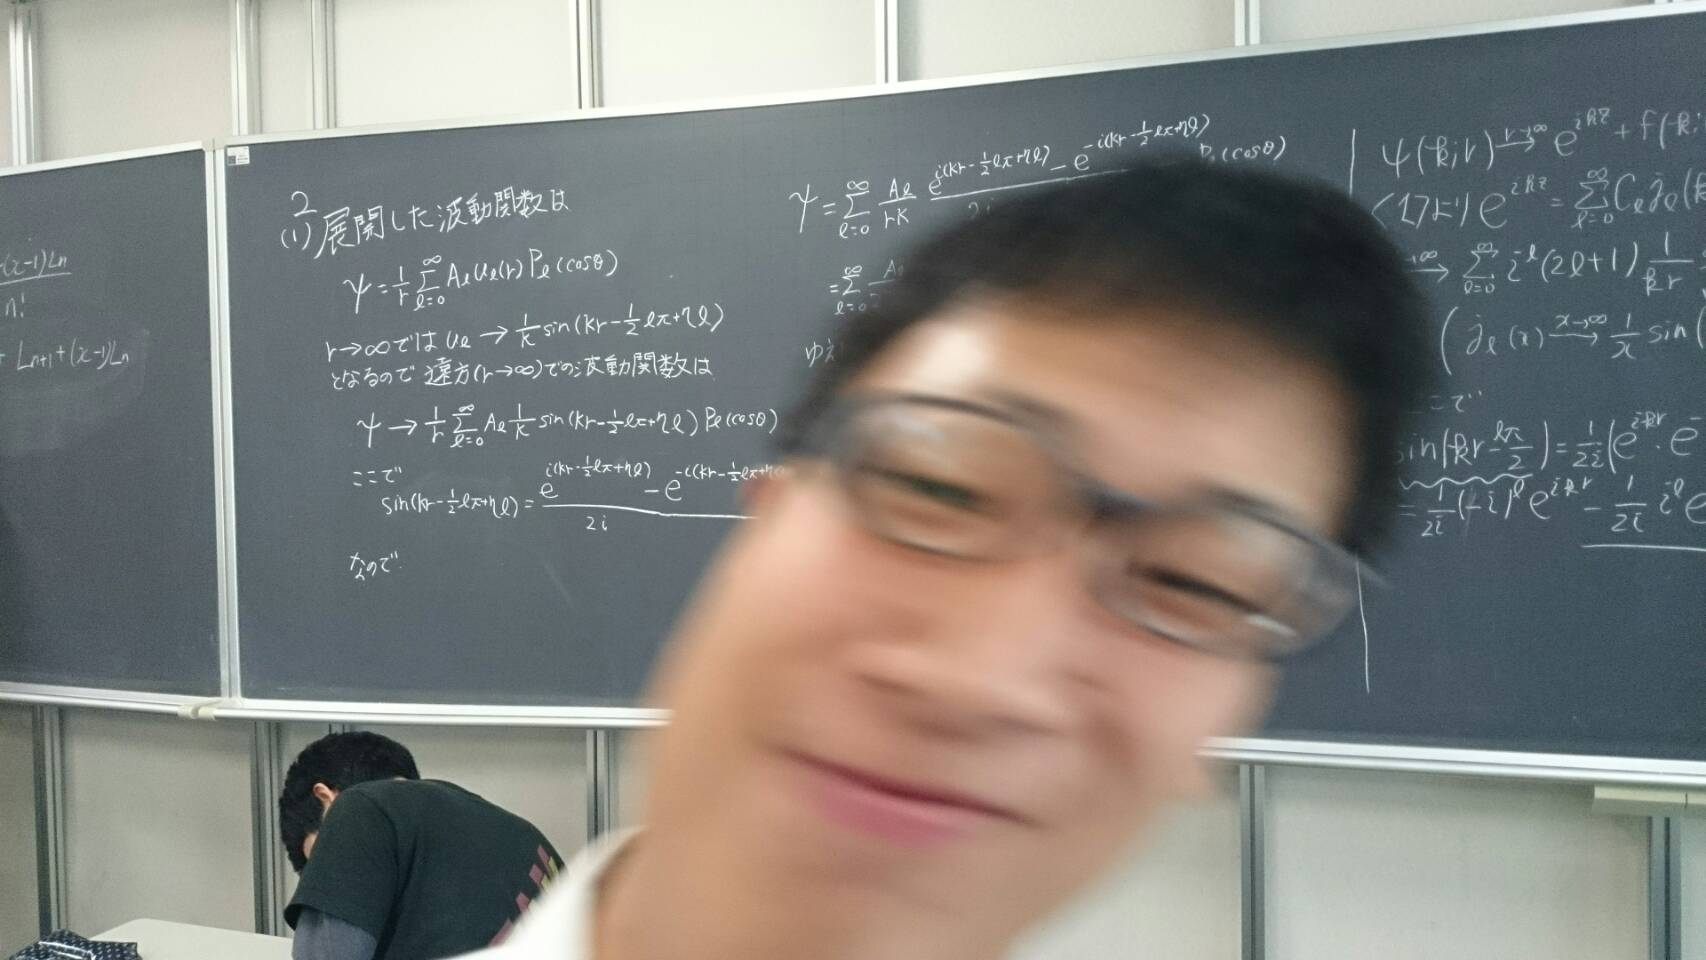
\includegraphics[clip,scale=0.1]{./kao}
\end{figure}

\vspace{5mm}

\begin{flushright}
\fontsize{15pt}{0cm}\selectfont{2030年5月2日}\\[1.3cm]
\end{flushright}
\begin{center}
\Large 専\ \ 攻\ \ 名\hspace{3cm}非言語学専攻\\[0.2cm]
\Large 学籍番号\hspace{3cm} 08082727aba\\[0.1cm]
\Large 氏\hspace{1cm}名\hspace{3cm}  網場翻怒 船長\\[1.3cm]
\LARGE 非言語大学\\
\end{center}
}
\makeatother

\title{\HUGE \it{概念論文}}
\date{\today}

\begin{document}
\maketitle
\thispagestyle{empty} %表紙にページ番号を出力しない
\newpage
\thispagestyle{empty}

%%%%%%%%%%%%%%%%%%%%%%%
%     概要
%%%%%%%%%%%%%%%%%%%%%%%
\newpage
\thispagestyle{empty}
{\huge 概要}\\
これはひどい\sf (´\_ゝ`)笑

%%%%%%%%%%%%%%%%%%%%%%%
%     目次
%%%%%%%%%%%%%%%%%%%%%%%
\newpage
\pagenumbering{roman}
\tableofcontents

%%%%%%%%%%%%%%%%%%%%%%%
%    セクション
%%%%%%%%%%%%%%%%%%%%%%%
\newpage
\pagenumbering{arabic}
%% 概念について
\section{概念}

\subsection{概念(広辞苑)}
事物の本質をとらえる思考の形成。事物の本質的な特徴とそれらの連関が概念の内容(内包)。概念は同一本質をもつ一定範囲の事物(外延)に適用されるから一般性をもつ。例えば、人という概念の内包は人の人としての特徴であり、外延はあらゆる人々である。しかし、個体(例えばナポレオン)をとらえる概念(個体概念・単独概念)もある。概念は言語に表現され、その意味として存在する。概念の成立については哲学に共通する内容をとりだし(抽象)、個々の事物にのみ属する偶然的な性質をすてる(捨象)ことによるとするのが通常の見解で、これに対立するものが経験から独立した概念(先天的概念)を認めた立場。\\

\subsection{概念の現状}
概念は、現在様々な使われ方をしている。一般に人間が上記の日本語の「概念」として用いられている場合と、次節で示される「概念そのものの概念」である。\\

\subsubsection{概念の概念}
概念の概念。それは通常の概念の概念ではなく、概念そのもの概念の本質に迫る概念である。現在、世界中の物理学者がこの問題について研究しており、様々な研究成果が報告されている。知らんけど。

\subsubsection{という概念}
近年ではあまり観測されない現象ではあるが、主に2015年、神戸大学の粒子物理研究室においてぐっさんにより観測された。何かしらの事象に対する呼応反応として「◯◯という概念。{\sf (´\_ゝ`)}笑」とか言ったりしてたっていう。

\subsubsection{概念方程式}
後述。知らんけど\sf(´\_ゝ`)

\newpage
\subsection{概念方程式}
\subsubsection{概念方程式(創世記)}
「概念の規格化」という概念が存在した。

\subsubsection{概念方程式(爆発)}
「概念の概念」という概念が爆誕した。

\subsubsection{概念方程式(整備)}
重症患者により概念についての整備がされ、以下で示される概念が明記された。

\begin{eqnarray}
{概念}^{概念}=?
\end{eqnarray}

\subsubsection{概念方程式(完成)}
重症患者により概念についての整備がなされた結果、以下で示される概念方程式が完成した。


\begin{eqnarray}
{概念1}^{概念2}={概念1}\times{概念2}
\end{eqnarray}

世界中の様々な重症患者達がこの概念方程式を解こうとしたが、未だかつて解かれておらず、概念の概念はどういう概念なのかとかそういう概念が概念概念していたという概念\sf{ (´\_ゝ`)}

\newpage
\subsection{概念方程式の解}
概念方程式を解いていく上で、概念における様々な定義の概念と公理の概念が必要であった。よってそれを以下に示す。

\subsubsection{定義}

\begin{eqnarray}
{概念1}\equiv G_{1}
\end{eqnarray}\footnote{概念の添字である数字は佐藤パラメータと呼ぶ}

\begin{eqnarray}
{概念2}\equiv G_{2}
\end{eqnarray}

\begin{eqnarray}
G_{1}^{G_{2}}=G_{1}G_{2}
\end{eqnarray}

\subsubsection{公理}
\begin{itembox}[c]{鈴木州のたこ鍋徹夜}
なんかもう一つ方程式ないとあかんやんとか言ってたら州がこんなん言いだした。
\begin{eqnarray}
\mathcal{L}(G_{i+1})=\frac{1}{G_{i}}
\end{eqnarray}
\end{itembox}

\begin{itembox}[c]{又吉先生のn}
後々なんかn=0であって欲しい場面が出てくるが、その理由を又吉先生に聞いたらこんなこと言ってた。
\begin{eqnarray}
n = 得ぬ = 0
\end{eqnarray}
\end{itembox}

\newpage
\subsection{解法}
概念方程式を徐々に解いていく。

\begin{eqnarray}
G_{1}^{G_{2}}&=&G_{1}G_{2}\\
\raisebox{.2ex}{.}\raisebox{1.2ex}{.}\raisebox{.2ex}{.}  G_{2}ln{G_{1}}&=&ln{G_{1}}+ln{G_{2}}\\
\end{eqnarray}

normalized to $G_{1}$

\begin{eqnarray}
ln{G_{1}}&=&\frac{1}{G_{2}}ln{G_{1}}+\frac{1}{G_{2}}ln{G_{2}}\\
\raisebox{.2ex}{.}\raisebox{1.2ex}{.}\raisebox{.2ex}{.} ln{G_{1}}(1-\frac{1}{G_{2}})&=&\frac{1}{G_{2}}ln{G_{2}}\\
\raisebox{.2ex}{.}\raisebox{1.2ex}{.}\raisebox{.2ex}{.} ln{G_{1}}\times (1-\frac{G_{2}-1}{G_{2}})&=&\frac{1}{G_{2}}ln{G_{2}}\\
\raisebox{.2ex}{.}\raisebox{1.2ex}{.}\raisebox{.2ex}{.} ln{G_{1}}&=&\frac{1}{G_{2}-1}ln{G_{2}}\\
\raisebox{.2ex}{.}\raisebox{1.2ex}{.}\raisebox{.2ex}{.} ln{G_{1}}&=&ln{G_{2}^{\frac{1}{G_{2}-1}}}\\
\raisebox{.2ex}{.}\raisebox{1.2ex}{.}\raisebox{.2ex}{.} G_{1}&=&G_{2}^{\frac{1}{G_{2}-1}}
 \end{eqnarray}

generalizing,

\begin{eqnarray}
\raisebox{.2ex}{.}\raisebox{1.2ex}{.}\raisebox{.2ex}{.} G_{i}&=&G_{i+1}^{\frac{1}{G_{i+1}-1}}
 \label{i1}
 \end{eqnarray}

so,it could be  derived the relation between $G_{i}$ and $G_{i+1}$.\\
\\
ところで、式\ref{i1}から一般概念$G_{n}$を求めようとした場合、簡単にはいかない。ここで、以下で示されるシステム「Wolfram Alpha」を導入する。\\

\newpage
\subsubsection{Wolfram Alpha}
Wolfram Alpha(WolframAlphaともWolfram|Alphaとも表記される)はウルフラム・リサーチが開発した質問応答システム。事実についての質問に対して、構造化されたデータを使って計算し、直接答えを返すオンラインサービスである。他の検索エンジンのように、答えを含んでいる可能性のあるドキュメントやウェブページのリストを返すわけではない[3]。このサービスは2009年3月に英国人科学者スティーブン・ウルフラムが発表し、同年5月15日に公開された[1]。
\begin{itemize}

\item 概要\\
ユーザはテキストフィールドに質問や計算リクエストを入力して送信する。Wolfram Alphaは知識ベースの精選された構造化データから答えと関連する視覚的情報を計算する。ゆえにWolfram Alphaは、多数の答えのインデックスを作成し、質問をいずれか1つに合致させようとするセマンティック検索エンジンとは異なる。\\
 Wolfram Alphaはコンピュータ代数、記号および数値計算、可視化、統計などの機能を網羅するウルフラムのフラッグシップ製品Mathematicaの上に構築されている。答えは通常読みやすい形の解で示される。\\
例:「lim(x->0) x/sin x」は正しい結果1に加え、ロピタルの定理を使った微分、プロット、そして級数展開を返す。\\
 Wolfram Alphaは自然言語を使った、事実についての質問にも答えることができる。例えば、「Where was Mary Robinson born?」(メアリー・ロビンソンが生まれた場所は?)や、より複雑な「How old was Queen Elizabeth II in 1974?」(1974年時点でエリザベス2世は何歳?)などである。 (ロビンソンについての答えには「Ballina, Mayo, Ireland」(アイルランドのメイヨー州バリナ)、バリナについてのさまざまな情報、ロビンソンについてのオンラインの略歴へのリンクが含まれる。エリザベス女王についての答えは「Result for start of 1974: 47 years」(1974年の始まりの時点で47歳)と略歴へのリンクである。)
複数のソースのデータを使って計算を行うこともできる。
例:「What is the fifty-second smallest country by GDP per capita?」(国民1人あたりの国内総生産が52番目に小さい国は?)と入力すると、ニカラグアで年1160ドルであると返される。\\
Wolfram|Alphaは少量の中核となる情報から推定を行う。 この点において、Wolfram Alphaは1980年代に始まった一般常識推論エンジンの開発に焦点をあてたプロジェクトCycとの多くの類似点がある。\\
データベースには、現在、現在および過去の天候情報など、何百ものデータセットが含まれている。このデータセットは2年以上かけて蓄積されており、今後も増える予定である。データセットの増加に従って答えられる問題の範囲も広がっていく予定である[4] 。

\item ライセンスパートナー\\
Wolfram AlphaはMicrosoft BingおよびDuckDuckGo検索エンジンの検索機能を提供している[5][6]。\\
Wolfram AlphaはAppleのSiri、DexetraのAndroid Irisから、事実に基づく質問に対する回答を受ける。\\
\item テクノロジー\\
Wolfram|AlphaはwebMathematicaとgridMathematicaを使って1500万行のMathematicaコードで書かれており[7]、1万個のCPU(この個数は起動に向けて拡張された)上で実行されている[8][9]。

\item 起動\\
 起動準備は中部標準時で2009年5月15日午後7時(16 May 2009 0:00 UTC)に始まり、Justin.tvでライブ放送された。高負荷問題を予想しながらも、その数時間後から公式起動する予定であった。このサービスは2009年5月18日に公式に起動した[10]。\\
Wolfram Alphaについては肯定的な評価がなされている[11][12]。 Wolfram Alphaの支持者の中には、将来性を評価する人や、現在の有用性よりWolfram Alphaが結果を導くその工程が重要なのだと指摘する人もいる[11]。
\item Wolfram Alpha Pro\\
2012年2月8日,Wolfram|Alpha Proが発表された[13]。これは月々の利用料によってユーザに追加機能を提供するものである。主な機能には、表形式、画像、音声、XML、何十もの特化した科学・医用・数学形式など、一般によく使われる多くのファイル形式をアップロードして自動的に解析することができるというものがある。その他には、拡張キーボード、CDFを使ったインタラクティブ機能、データのダウンロード、グラフィックスや表を含む結果をカスタマイズして保存できる機能などがある[14]。
Wolfram Alpha Proの新しいプレミアム機能の導入に伴い、無料ページにいくつかの変更点が加わった。
無料サイトの広告が増えた。
テキストとPDFによるエキスポート機能を利用するためには、無料アカウントが必要になった。
時間のかかる計算のための計算時間延長のリクエストは以前は無料[15]であったが、購読者のみが対象となった[16]。
\end{itemize}


\newpage
以上のWolfram Alphaをいそべっちがぐぐってなんか計算してくれたのを参考$\sf{ (´\_ゝ`)}$にし、計算を続けた。その結果、図\ref{wolfram}のような結果となった。\\
\begin{figure}[H]
\centering
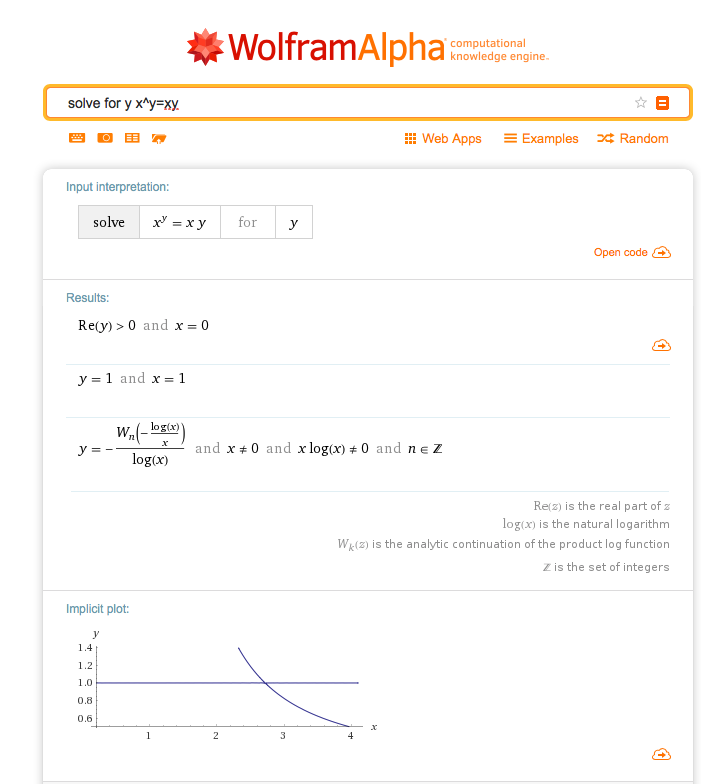
\includegraphics[clip,scale=0.35]{wolfram.png}
    \caption{Wolfram Alpha}
    \label{wolfram}
\end{figure}

これより、式\ref{i1}から一般概念$G_n$を求めると式\ref{i2}で表される。

\begin{eqnarray}
G_{i+1}=-\frac{W_{n}\left( -\frac{logG_{i}}{G_{i}}\right)}{logG_{i}} \ \ \ \ 
\label{i2}
 \end{eqnarray}

ここで$W_n$はランベルトのW関数である。

\newpage
\subsubsection{ランベルトのW関数}
数学におけるランベルトW函数(ランベルトWかんすう、英: Lambert W function)あるいはオメガ函数 ($\omega$function), 対数積(product logarithm; 乗積対数)は、函数 f(z) = zez の逆関係の分枝として得られる函数 W の総称である。ここに ez は指数函数で z は任意の複素数とする。すなわち W は z =$f_{−1}(zez)$=W(zez) を満たす。
上記の方程式で z' = zez と置きかえれば、任意の複素数 z' に対する W 函数(一般には W 関係)の定義方程式
\begin{eqnarray}
z'=W(z')e^{W(z')} 
\label{i3}
 \end{eqnarray}

を得る。
函数fは単射ではないから、関係Wは(0を除いて)多価である。仮に実数値のWに注意を制限するとすれば、複素変数zは実変数xに取り換えられ、関係の定義域は区間x$\leq$−1/eに限られ、また開区間 (−1/e,0) 上で二価の函数になる。さらに制約条件として W$\leq$−1 を追加すれば一価函数$W_{0}(x)$が定義されて、$W_{0}(0) = 0$および$W_{0}(−1/e) = −1$を得る。それと同時に、下側の枝は W$\leq$−1であって、$W_{−1}(x)$と書かれる。これは$W_{−1}(−1/e)=−1$から$W_{−1}(−0)=−\infty$まで単調減少する。
ランベルトW関係は初等函数では表すことができない。ランベルトWは組合せ論において有用で、例えば木の数え上げに用いられる。指数函数を含む様々な方程式(例えばプランク分布、ボーズ-アインシュタイン分布、フェルミ-ディラック分布などの最大値)を解くのに用いられ、また$y'(t) = ay(t − 1)$のような遅延微分方程式(英語版) の解としても生じる。生化学において、また特に酵素動力学において、ミカエリス-メンテン動力学の経時動力学解析に対する閉じた形の解はランベルトW函数によって記述される。知らんけど\sf (´\_ゝ`)笑

\newpage
\subsubsection{一般概念解}
以上を用いて一般概念解を求めていく。\\
まず、概念方程式より

\begin{eqnarray}
G_{i}^{G_{i+1}}&=&G_{i}G_{i+1}
 \end{eqnarray}

一方で、鈴木州のたこ鍋徹夜より、
\begin{eqnarray}
左辺&=&\mathcal{L}(G_{i+1})\nonumber\\
&=&\int^{\infty}_{0}G_{i+1}e^{-it}dt\nonumber\\
&=&G_{i+1}\int^{\infty}_{0}e^{-it}dt\nonumber\\
&=&G_{i+1} \frac{1}{-i} \left[ e^{-it} \right]^{\infty}_{0} \nonumber\\
&=&-iG_{i+1}\\
\raisebox{.2ex}{.}\raisebox{1.2ex}{.}\raisebox{.2ex}{.} \ -iG_{i+1}&=&\frac{1}{G_{i}}\nonumber\\
\raisebox{.2ex}{.}\raisebox{1.2ex}{.}\raisebox{.2ex}{.} \ G_{i}G_{i+1}&=&i
\label{i4}
\end{eqnarray}

となる。\\
また、又吉先生のnの概念を導入するとn=0になり、ランベルトのW関数に対して$W_{0}$の0を中心とするテイラー級数を逆に解いて近似すると

\begin{eqnarray}
W_{0}(x)&=&\sum^{\infty}_{n=0}\frac{(-n)^{n-1}}{n!}x^n\nonumber\\
&=&x-x^2+\frac{3}{2}x^3-\frac{8}{3}x^4+\frac{125}{24}x^5...\nonumber\\
&\sim&x
 \end{eqnarray}

となるので、式\ref{i2}について、
\begin{eqnarray}
G_{i+1}&=&-\frac{W_{0}\left( -\frac{logG_{i}}{G_{i}}\right)}{logG_{i}} \nonumber\\
&=&\frac{-1}{logG_{i}}\times -\frac{logG_{i}}{G_{i}}\nonumber\\
&=&\frac{1}{G_{i}} \nonumber\\
\raisebox{.2ex}{.}\raisebox{1.2ex}{.}\raisebox{.2ex}{.} \ G_{i}G_{i+1} &=& 1
\label{i5}
 \end{eqnarray}

と表される。\\
以上の式\ref{i4}、\ref{i5}より、
\begin{eqnarray}
\Large{i=1}
 \end{eqnarray}

となり、概念の概念から、「愛は一つ」ということが示された。またっっっっっっ\sf{ (´\_ゝ`)}笑

%%%%%%%%%%%%%%%%%%%%%%%%%%%%%%%%%%%%%%%%%%%%%%%%%%%%%%%%%

%% ATM理論
\section{The theory of ATM particle}

\subsection{何がしたいのか{\sf (´\_ゝ`)}笑}
\subsubsection{その時歴史が動いた}
事の発端はセブンイレブンである。我々が工学部にあるセブンイレブンでなんか飯とか買おうかな、とりあえずドリンク買うか、みたいな感じになっていると、急速に図\ref{ATMATM}のような現象が観測された。

\begin{figure}[H]
\centering
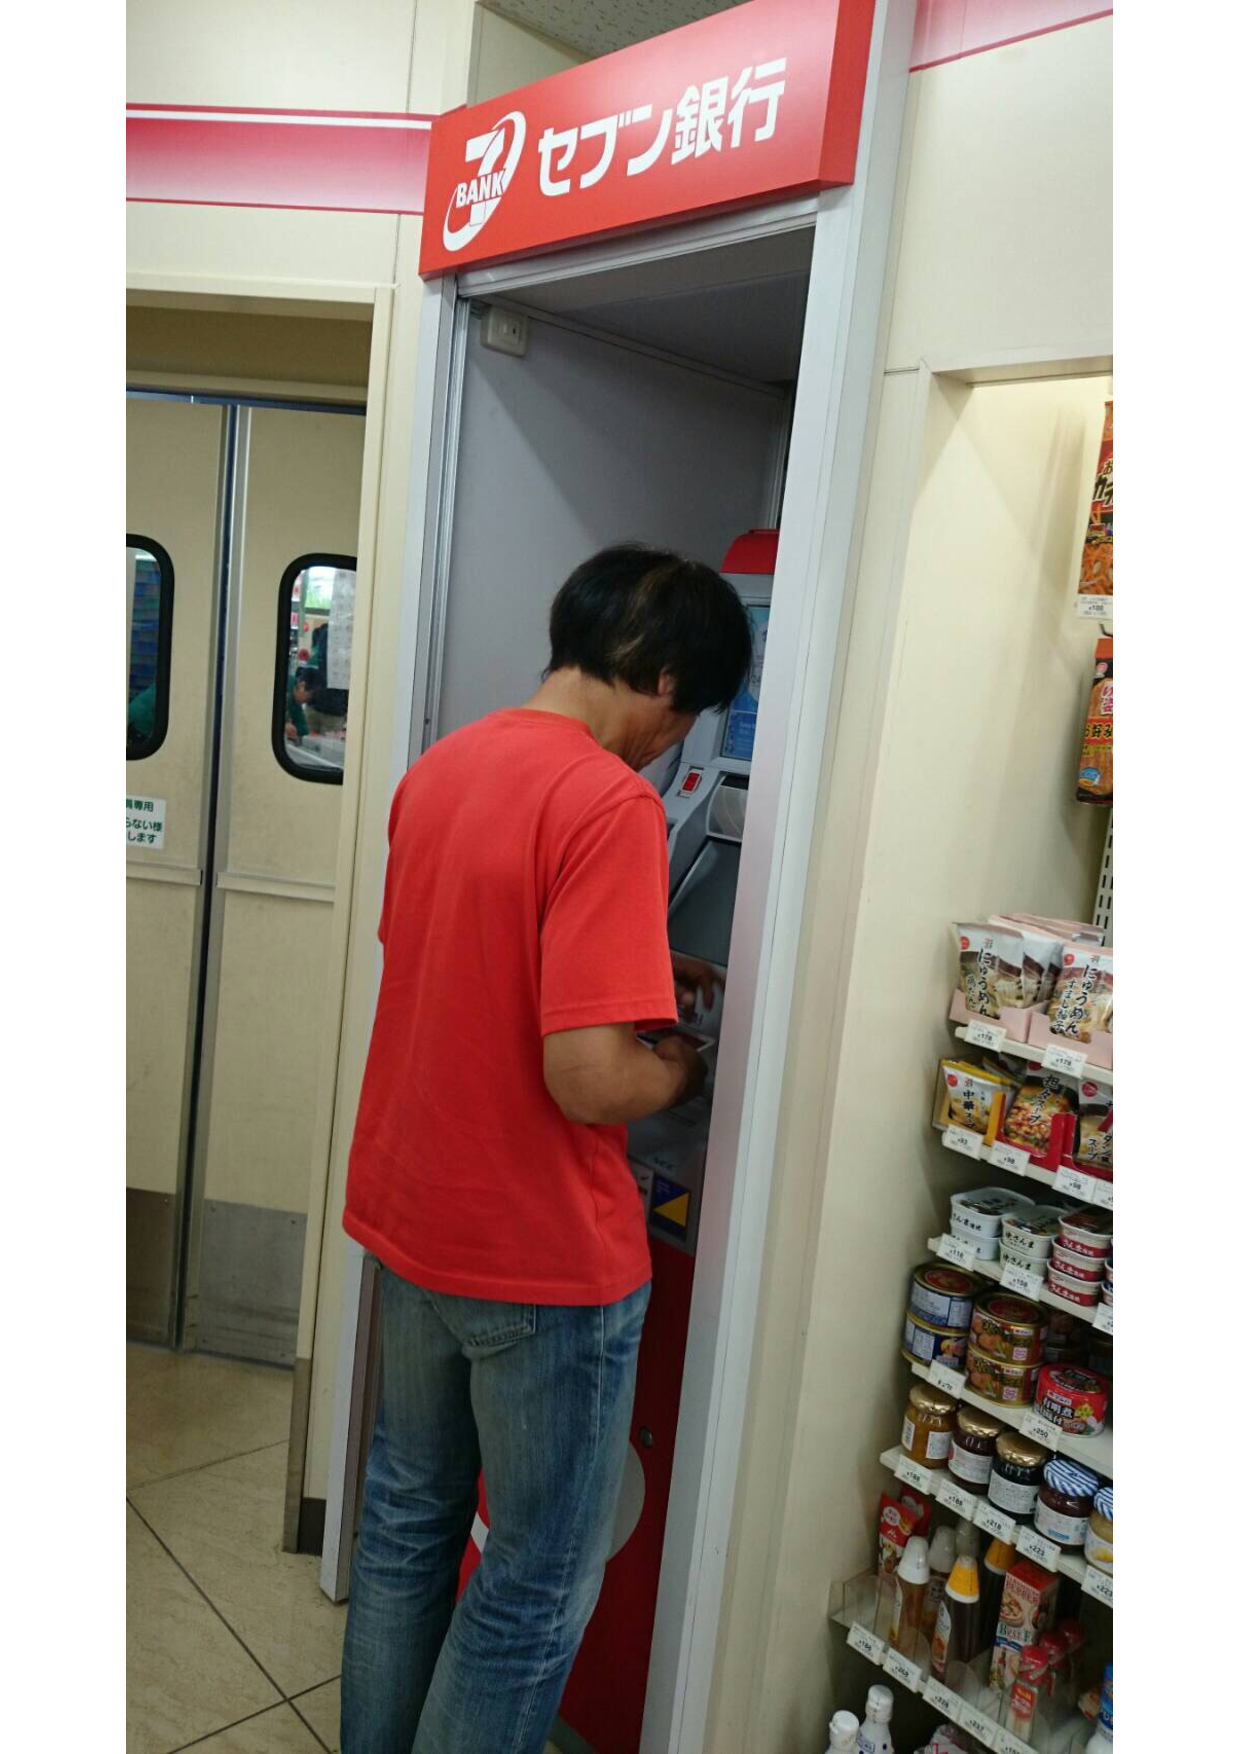
\includegraphics[clip,scale=0.35]{ATMATM.pdf}
    \caption{その時歴史が動いた}
    \label{ATMATM}
\end{figure}

これはひどい。あのATM\footnote{鈴木州}がATM\footnote{現金自動預け払い機}で金を降ろしているのである。

\subsubsection{当時の状況}
この奇妙な現象が観測されたとき現場には多くの生物が存在しており、我々は取材を通じてその当時の状況についての情報を得ることができた。ここではその一部を紹介する。\\

まずはこの人。\\

\begin{itembox}[c]{アバポンヌ船長さん(年齢不詳)}
まず、爆笑しました。何してんねや、コイツと。そして、「預金いくらなんすか」と問いかけると「あぁん」としか返ってこず、除き込もうとすると体でガードする。その時にはさほど大金は引き出しておりませんでした。ATMを利用している人をみて爆笑したのはあれが最初で最後です。
\end{itembox}
\\

さらに、あの伝説の人物にも話を聞くことができた。\footnote{非言語大学特任教授。バTeXの権威。BaTeXを10年前に作ったが、誰も使わず。しかし、1人で細々とバージョンアップを重ね、このBaTeXが世界に広がる事を夢見て死んでいく予定の教授。} \\
\begin{itembox}[c]{バタバ田 テフ夫さん(83) }
$一般的にATMはお金を預けて引き出すものであるが、神戸大学自然科学3号館3階在住のATM(区別するため仮に\overline{ATM}とする。)はこれとは逆の性質を持ち、お金を借り入れることができる。
このことから一部では\overline{ATM}がATMの反物質ではないかという理論予想がされていた。
これを実験的に確かめる方法は容易で、ATMと\overline{ATM}が衝突した時に対消滅を起こせば\overline{ATM}はATMの反物質であると断定できる。
しかしATMは反応断面積・ルミノシティ共に非常に小さいため、これを観測するのは至難の技であり、今日(こんにち)まで観測を行った人間は誰一人としていなかった。
そしてこの日、我々は奇跡的にその観測を成功させたのである。
ところが、ATMは消滅することなく、お金をATMから\overline{ATM}に与える形での相互作用を起こした。
こうして前述の理論は白紙に戻ったわけであるが、この観測がATM理論のブレイクスルーとなることを私は期待している。$
\end{itembox}

このとき我々はこの現象を以下のように表現した。\\
\begin{center}
{\LARGE \mc ATMとATMの衝突が起こった。{\sf (´\_ゝ`)}}
\end{center}

この時以降、我々はこの現象をATM ATM collisionと名付け、より詳細な議論がなされるようになった。


\newpage
\subsection{詳細な研究}

\begin{itembox}[c]{非言語大学名誉教授 竹田 小川之介 (23)}
ATMの振る舞いを観察するためにセブンイレブンへ入店した際、新粒子の痕跡が私の心の中の検出器に残りました。その前後3イベントを精査すると、セブン銀行と反応する新粒子らしき、trackとなる現象を観測できました。量子電磁力学、ワインバーグ・サラム理論、量子色力学といった、実験によって検証されている理論を超越した仮説上の理論が、私のなかで産声を上げました。それは現在、場の量子論を超越した基礎理論として研究されていると言われています。
この新粒子に触れたものはみな不幸になると、予言されております。\\
それは " 口座残高零円理論 "として予言されており、この理論の裏付けを進めるため、ATLAS(アバポンヌ・トストス・クルパァゴ・アブラ・サテ)実験では500度目のアップグレードを計画しています。
\end{itembox}

\newpage
\subsection{ATLAS}
ここで、前節ででてきたATLASについて紹介する。一言でATLASと言っても世界には様々なATLASの説が存在するため、本論文では定説である3つのATLASについて述べる。

\subsubsection{FUJITSU Software ATLAS}
ATLASは業界最高水準の翻訳精度を誇る翻訳ソフトです。高品質翻訳ソフトの定番として、発売以来数多くのお客様に支持され、No.1のシェアを維持してきました。Microsoft Word、Excel、PowerPoint、PDFなどのドキュメントの翻訳から、メール、ホームページの翻訳まで幅広いシーンでご利用いただけます。

\begin{figure}[H]
\centering

\includegraphics[clip,scale=0.5]{ATLAS1.pdf}
\caption{FUJITSU Software ATLAS}
\end{figure}

\subsubsection*{特徴}
富士通独自の高品質翻訳エンジン:翻訳ソフト選びの最も重要なポイントは翻訳精度です。 ATLASは、富士通が長年にわたり改善を重ねてきた翻訳エンジンと基本辞書により、使い始めから精度の高い翻訳を導き出します。
\paragraph{翻訳エンジン}
「翻訳エンジン」は文章を解析し訳文を生成する翻訳ソフトの要です。 ATLASは、文章の意味を把握しながら翻訳する「意味処理方式」や、日本語と英語の違いに着目し、 自然な訳文を出す「概念\footnote{1章参照}変形」を採用しています。
\paragraph*{概念変形}
日本語と英語の言葉の違いに着目し、主語・目的語を入れ替えたり、態や時勢を替えたりします。

\begin{figure}[H]
  \centering
  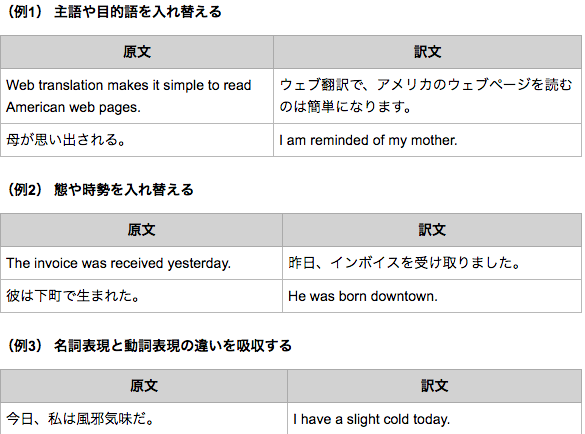
\includegraphics[clip,scale=0.5]{ATLAS2.png}
  \caption{概念変形}
\end{figure}

\newpage
\subsubsection{ATLAS(Abaponnu Tosutosu kuLupargo Abra Sate)}
\subsubsection*{概要}
鈴木州原子核研究機構 (Atsumu Nuclear Association:通称ANA) にある検出器・検出器衝突型円形加速器 (Large detector vs detector Hardware Collider:通称LHC) では、検出器同士を加速し衝突させている。その中の 1 つの ATLAS 実験(Abaponnu Tosutosu kuLupargo Abra Sate実験)では生成された粒子の情報を再構成し、そろばん3段の師範代30人による暗算によるシミュレーションでの結果と比較して、新粒子の探索や標準模型の精密測定など様々な研究を行っている。  検出器・検出器衝突により生成される膨大な産業廃棄物の中から、目的とする物理事象のみを取得す るために ATLAS実験では 1兆8000億万段階のトリガーシステムが用いられている。その 1 段階目に位置するレベル 1 トリガーは、昼夜を問わず(時給1300円で雇われた)アルバイトが「この粒はヒッグスだ!」「この粒はZ粒子だ!」と賑やかにワイワイと、産業廃棄物(いわゆるゴミ)の中から、選別作業を行っている。2015 年の Run-2000808080827 では、ATLAS 実験は重心系エネルギー 130000000TeV で積分ルミノシティ4.0fb−1 の実験データを取得した。2016 年以降のルミノシティの増加に伴い、今のままだとさらにトリガーレートが増えることが予想されている。そのためさらに数多くのバイトを雇い、一粒一粒、素粒子の選別作業を頑張る予定です。笑顔の絶えない明るい職場です!あなたも一度どうですか?

\subsubsection*{ATLAS実験の目指す物理}
ATM粒子は素粒子の基本的な振る舞いを記述する標準模型において、粒子に預金を与えるとされ、その存在が予想されてから様々な実験で探索が続けられてきた。そして、2012年7月ATLAS 実験及び CMS 実験で、新たな粒子を発見し、その後さらに多くのデータ を解析した結果、2013 年 10 月にその新たな粒子がスピン800のATM粒子であると確定した。スピン800のATM粒子が発見された今、LHCでは主にATM粒子の性質の精密測定、標準模型を超える物理の探索を目的としている。


\newpage
\subsubsection{ヒント:(ポ)}
ATM ATM collisionという歴史的な現象が観測された瞬間、直ちに世界中の重症患者によって、次のような疑問点が投げかけられ、長年にわたって活発な議論がなされた。

\begin{itemize}
\item 何をしているのか{\sf (´\_ゝ`)}
\item お金どんくらい持ってるんやろ{\sf(´\_ゝ`)}
\end{itemize}

もちろん国立大学法人である神戸大学の助教という立場であるATMのお金に関しては、だいたいなんかググったら給料とかは調べられるらしい。ただし、等級によって多少の違いがあるため厳密にはわからない。%\cite{yano}
ましてや、給料はわかっても普段の出費などがあるため持っているお金、すなわち「預金残高」に関して詳細な研究は未だなされてはいない。
そこで、我らが(ポ)\footnote{非言語大学教授}によって次のような定理、またそれに準ずる現象が預言された。




\begin{itembox}[c]{第一定理:ATM場}
ATM場は預金とともに、指数関数的にATM粒子が増えていく。
\end{itembox}

\begin{itembox}[c]{第二定理:ATM粒子}
ATM粒子とATM粒子は預金の二乗に反比例した力を及ぼし合う。\\
ATM粒子とATM粒子が一定距離近づくと、老人ホーム場ができる。
\end{itembox}

\begin{itembox}[c]{第三定理:老人ホーム場}
無限の深さの井戸型ポテンシャルを持って、ATM粒子がそこに捉えられると負の方向にずっと落ち込む。\\
ATM力の単位は圧力と同じ。オーダーは$~1 atm$
\end{itembox}

\begin{itembox}[c]{第四定理:ATM力}
$預金=m\times O \times N \times e ^{ -y }$
\begin{itemize}
\item m: mass [kg]
\item O: ATM定数
\item N: 粒子数
\item y: distance [m]
\end{itemize}
\end{itembox}

\newpage
\subsubsection{ヒント:(マ)}
\label{mata}
また、ATM定数について、又吉氏によって以下の理論が提唱された。
\begin{itembox}[c]{又吉理論}
$O(N) = マイナンバー = 12ケタ = 10^{12}$
\end{itembox}

\subsubsection{ATM ATM collisionの解}
上記の様々な予言により、ATM ATM collision event の解析が進められた結果、以下のようになった。\\
まず、第一定理より、
\begin{eqnarray}
預金 &=& deposit\nonumber\\
&=& d
\end{eqnarray}

また、第三定理は、ATM ATM collisionが起こる距離$L$に対し、ATMのポテンシャルは以下のように表現できる。

\begin{eqnarray}
V(y)=\left\{ \begin{array}{ll}
0 & (y<0,  L<y) \\
-\infty & (0<y<L) \\
\end{array} \right.
\label{ATMpotential}
\end{eqnarray}
\\
図\ref{SqureWell}にように解釈できる。

\begin{figure}[H]
\centering
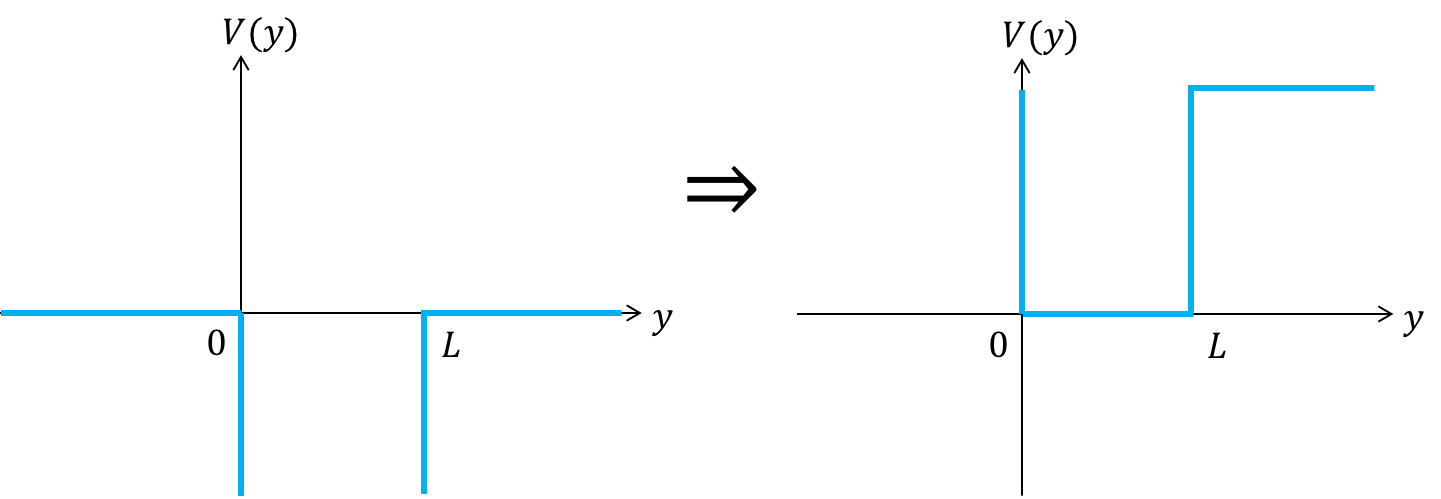
\includegraphics[clip,scale=0.4]{SqureWell.png}
\caption{(左図)ATM ATM potential の概念。\
(右図)こんな感じの場合と同じやしこれで考える}
\label{SqureWell}
\end{figure}

これは、ATMとATMの距離$y$が$L$となると負の方向にずっと落ち込むことから、$y=L$のとき$deposit$が発生すると考えることができる。すなわち、
\begin{eqnarray}
L = d
\label{Ld}
\end{eqnarray}

と表現できることがわかる。これはすなわち、第二定理を表していることに他ならない。\\
式\ref{ATMpotential}、\ref{Ld}より、第三定理をまとめると式\ref{ATMpotential_new}のようになる。
\begin{eqnarray}
V(y)=\left\{ \begin{array}{ll}
0 & (y<0,  d<y) \\
-\infty & (0<y<d) \\
\end{array} \right.
\label{ATMpotential_new}
\end{eqnarray}

次に、式\ref{ATMpotential_new}について、シュレディンガー方程式を解く。シュレディンガー方程式

\begin{eqnarray}
\left[ -\frac{\hbar^{2}}{2m} \frac{\partial^{2}}{\partial y^{2}} + V(y) \right] \psi(y)= E \psi (y) 
\label{schoredinger}
\end{eqnarray}

を解くと以下のようになる。

\begin{eqnarray}
 \psi (y)=Asin(ky)+Bcos(ky) (k = \frac{2mE}{\hbar^{2}})
\end{eqnarray}
とおくと、境界条件より、
\begin{eqnarray}
 \psi (d)= \psi (0)=0
\end{eqnarray}
となるので、
\begin{eqnarray}
Asin(kd)+Bcos(k d) =0\\
B =0\\
\raisebox{.2ex}{.}\raisebox{1.2ex}{.}\raisebox{.2ex}{.}Asin(kd)=0
\end{eqnarray}
A$\neq$0より、
\begin{eqnarray}
sin(k d)=0\\
\raisebox{.2ex}{.}\raisebox{1.2ex}{.}\raisebox{.2ex}{.} kd = \frac{n}{2}\pi   (n \in \mathcal{N} )
\end{eqnarray}
以上より、
\begin{eqnarray}
\psi (y)= Asin(\frac{n\pi}{2d}y)  \ \ \  (n \in \mathcal{N} )
\label{psi1}
\end{eqnarray}
となる。
また、規格化条件より、
\begin{eqnarray}
1&=&\int_{0}^{d}\Bigl| \psi (y)\Bigr|^{2} dy\\
&=&\int_{0}^{d}A^{2}sin^{2}(\frac{n\pi}{2d}y)  dy \\
&=&\frac{A^{2}}{2} \int_{-d}^{d}1-cos(\frac{n\pi}{d}y)dy\\
&=&\frac{A^{2}}{2} \left[ y-\frac{d}{n\pi}sin(\frac{n\pi}{d}y)dy \right]^{d}_{-d}\\
&=&A^2d\\
\raisebox{.2ex}{.}\raisebox{1.2ex}{.}\raisebox{.2ex}{.} A&=&\sqrt{\frac{1}{d}}
\end{eqnarray}

となる。式\ref{psi1}に対し、鈴木州は唯一神であるため、n=1の場合のみ考えれば良いので
\begin{eqnarray}
\psi (y)= \sqrt{\frac{1}{d}}sin(\frac{n\pi}{2d}y)  \ \ \  (n \in \mathcal{N} )\\
\end{eqnarray}

となる。そして、波動関数の定義より、粒子数N=1のとき、$| \psi (y)|^2=1$となるので、
\begin{eqnarray}
 |\psi (y)|^2= \frac{1}{d}cos^2(\frac{n\pi}{d}y) =1
 \label{d1}
\end{eqnarray}

となる。\\
次に、第四定理により、N=1を適用し、
\begin{eqnarray}
N&=&\frac{1}{mO} \times d \times e^{y} =1\\
\raisebox{.2ex}{.}\raisebox{1.2ex}{.}\raisebox{.2ex}{.} y&=&\ln\frac{mO}{d}
\label{d2}
\end{eqnarray}

となる。\\
したがって、式\ref{d1}、\ref{d2}より、yを消去し、
\begin{eqnarray}
 \frac{1}{d}cos^2(\frac{\pi \ln mO}{d}) =1
 \label{d3}
\end{eqnarray}

ここで、又吉理論(\ref{mata})により、

\begin{eqnarray}
 \pi \ln (mO) &=& 3.14\times \ln (60\times10^{12})\nonumber\\
 &=&99.668175746928...\nonumber\\
 &\sim&100
\end{eqnarray}

となるので、式\ref{d3}をdについて解くと、

\begin{eqnarray}
d \sim 1 \ [\rm{kg}]
\end{eqnarray}

となる。預金dの重さが1 kg、これはすなわち金額にして1000万円に相当する。\\
\large{以上より、州の預金残高のオーダーは1000万円である。\sf(´\_QED`)笑}


%%%%%%%%%%%%%%%%%%%%%%%%%%%%%%%%%%%%%%%%%%%%%%%%%%%%%%%%%%%%%%%%%%%

%%%% 非言語大学
%!TEX root = ../../main.tex
%==============%
\chapter{非言語大学}
\label{sec:HigengoUniv}
\index{ひげんごだいがく@非言語大学}
%=============%

言語とは、人類史が始まって以来の最大の発明として、コミニュケーションのツールとして非常に重要な役割を果たしている。
現代はグローバルな社会であり、国家間の関係もより緊密になり、国交・経済・文化の結びつきが一層強固になってきている。
特に国交・経済の分野においては、正確なコミニュケーションと迅速なやり取りが必要不可欠であり、英語(English)が世界標準言語として広く使用されており、本国日本の言語である日本語は非常にマイナーな言語と見なされている。

図\ref{Fig:LanguageMap}に現在世界で使用されている言語族の分布図を示す。
英語に関する言語族が広く分布していることが分かり、対象的に日本語は非常に限られた地域で特異に発展してきた文化であることが推測される。
しかし国際標準言語である英語にも、イギリス英語とアメリカ英語に代表されるように、いわゆる「方言」としての発音・文法の違いがメディア等でも様々に取り上げられている。
また新興国で使用されている英語はさらに形の崩れたものとなっており、スムーズなコミニュケーションが不能になる場面も多々見受けられる。
大きな差に始まり微妙な差も、この国際社会においては、正確なコミニュケーションに対する大きな障壁になりつつある。
過去幾度となく人類が起こしてきた戦争を回避し、今後人類が国境のない世界・平和の訪れた世界を見据えるためには、より柔軟な、かつ誰が使用しても差異のない完璧な言語が求められると考えられる。

%%%%%%%%%%%%%%%%%%%%%%%%%%%%%%%%%%%%%%%%%
\begin{figure}[h]
\centering
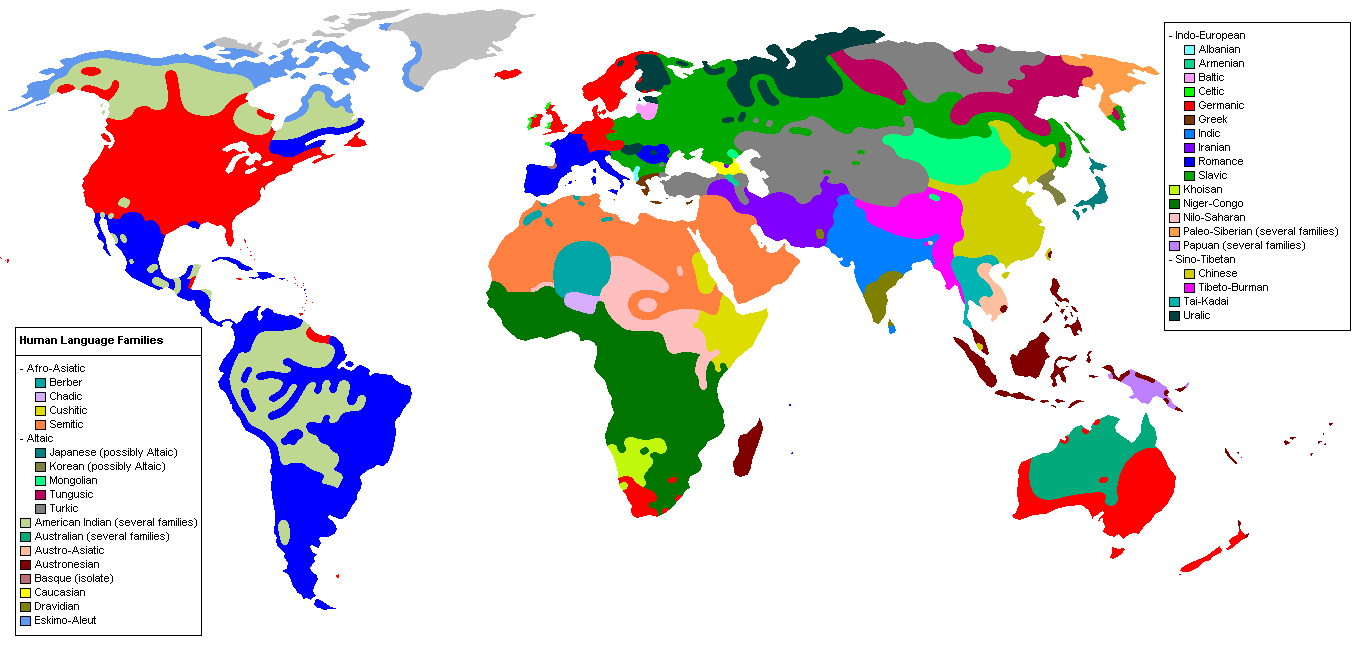
\includegraphics[width=0.8\textwidth]{./section/HigengoUniv/figures/Human_Language_Families_Map.png}
\caption{世界言語マップ[https://www.tefl-iberia.com/blog/human-language-map/]}
\label{Fig:LanguageMap}
\end{figure}
%%%%%%%%%%%%%%%%%%%%%%%%%%%%%%%%%%%%%%%%%

一つの人類の解として、エスペラント語が用意されている[http://www2.sal.tohoku.ac.jp/~gothit/espj.html]。この言語は、中立で使いやすい国際共通語を目指し、1887年にユダヤ人眼科医ザメンホフ (L.L. Zamenhof)が提唱したもので、民族の言語や文化をその歴史的遺産として尊重し、それぞれの言語や文化の違いを越えて人々がコミュニケーションできるようにするために橋渡しの役目を果たすことを目的として作成されたものである。
人工的に使用された言語であるエスペラントの使用者(エスペランティスト)はそれぞれ個人として平等の立場に立って話し合うことができ、将来的に非常に重要な意義を持つ言語であると考えられている。
この様に、言語を学問として捉えることは、今後の世界の在り様を考えるためにも非常に重要な入り口となっていることが分かり、近年言語学が加速発展してきている。

言語学者は、世界の言語の特徴や特質を研究し、言語を成り立ちや構造、変化・変遷、分布、比較などさまざまな角度から捉えることで言語に対する理解を深めていく。学問領域は、主に言語の本質を探るための「意味論」「語彙論」「文法論」「文字論」「音韻論」などから成りたっている。
しかし、エスペラント語に代表されるような人工言語にも限界があり、つまり、新しく記憶し直さなければならない、という障壁が、学習への大きな足かせとなっている。
そこで、言語学習を困難にする非常に大きな要因の一つを取り除くため、2012年に、世界で初めて言語に頼らない言語コミュニケーション、いわゆる非言語コミュニケーションが提唱された。これに起因し、非言語学はその学問領域を膨張し拡大されていき、いまや世界の約99\%の人口は非言語コミュニケーションを行っていると考えられている。

特に、非言語の研究は2012年来の長い伝統と優れた成果を有している一方で、他の言語と相対化させる努力が十分ではなく,(i) 世界諸言語の中でどのような言語なのか、(ii) 一般言語学・言語類型論の視点から見ると、どのような知見が得られるのか,(iii) 非言語の研究が世界諸言語の研究や一般言語学・言語類型論にどのように貢献するのか,いまだ十分に明らかにされておらず、現代の非言語研究には、一般言語学や言語類型論研究にどのように貢献できるのかという「内から外を見る」視点と、一般言語学や言語類型論研究が非言語の分析にどのような知見をもたらすかという「外から内を見る」視点が必要である。
そこで、非言語学を専門とし、国際的に協力していくために、2012年に非言語学が提唱されてから約数年後に、非言語大学が設立された(建立は1993年である、後述)。
非言語大学から発信される非言語研究プロジェクトは、多数の視点から非言語の言語事実を分析することにより、世界の諸言語と対照させて非言語の特質を明らかにし,それにより非言語研究の国際化を図ることを主たる目的としている。非言語の音声・音韻,語彙・形態,文法,意味の構造を,言語獲得 (第一言語獲得,第二言語習得) はもとより,言語に関係する他の学問分野 (心理学,認知科学他) との接点・連携をも視野に入れて,対照言語学・言語類型論の観点から分析することにより,諸言語間に見られる類似性 (普遍性) と相違点 (個別性・多様性) を明らかにしている。

本章では非言語大学の歴史に始まり、最先端の非言語研究の大きな成果の一つである、非言語コミュニケーションの詳細を述べると共に、受験生へのエールをまとめる。


%非言語とは現在確立されている一般的な言語に頼らず、意思疎通を図るための手段である。
%人類発生の起源を辿れば非言語コミュニケーションに行き着く。
%つまり非言語とは人類と深い関係のある概念である。
%しかし、現代情報社会において最も重要なことの一つに「情報の正確さ」という概念が考えられ、それを実現するためには正確な言語コミュニケーションが必要となってくる。
%そのため近代科学史において非言語を研究するということは非常にマイナーな学問であった。

%しかし、1993年建立の非言語大学(Higengo University)は、非言語研究の第一人者である小川田氏により創設された、世界ではじめての国際的な非言語通信教育制の研究機関であり、全世界人口のうち約100億人が入学希望を出している超有名大学である。


%~~~~~~~~~~~~~~~~~~~~%
\section{非言語とは}
\index{ひげんご@非言語}
%~~~~~~~~~~~~~~~~~~~~%
非言語には学問上、2種類に分類することができ、一つは「言語に非ず」の意味に由来する非言語、もう一つは「"非"常に発達した"言語"」としての非言語である。
いまや世界標準になりつつある事実からは、このどちらの意味も非言語にとって正しい意味を持っていると推測される。
特に、人類は幼児の時には母国語を覚えるよりも前に非言語を覚えている、と考えられており、成長に従い、大人に倣い母国語を発達させるのである。
図\ref{Fig:HigengoDevelop}に着床から出産までの非言語の発達を示す。
受精して初めて、幼生はアブラ関連の単語を発することができると考えられている。
しかし非常に高周波でアブラと発するため、通常の検診では言語を検知することは困難であり、また母体もそれに気づくことは極めて稀である。
もしお腹が揺れているような感覚に襲われた場合は、殆どの場合幼生の発する「アブラ」が起因すると考えられており、初診の超音波検診による高周波に反応しているとも考えられている。
\begin{figure}[h]
\centering
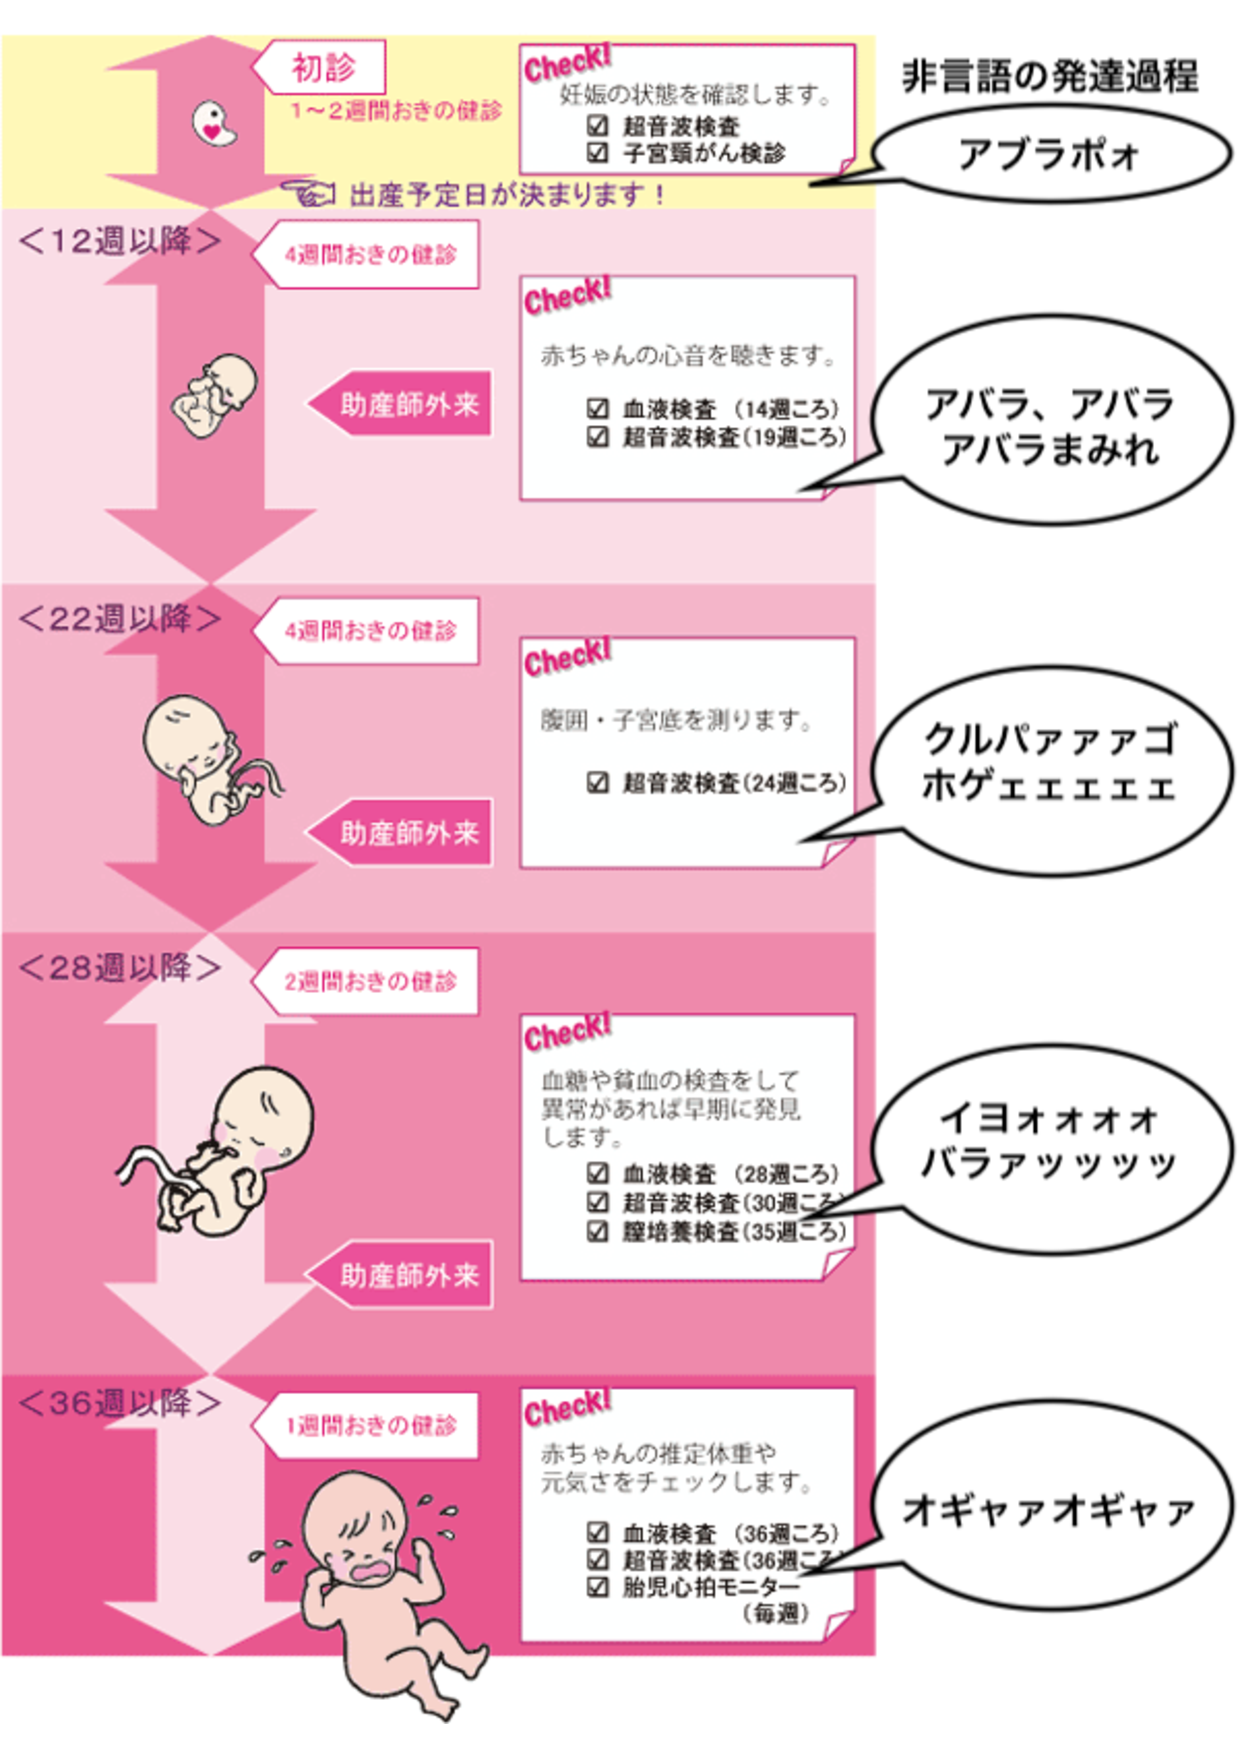
\includegraphics[width=0.5\textwidth]{./section/HigengoUniv/figures/baby.pdf}
\caption{着床から出産に至るまで、幼生が獲得する非言語のチャート図。出産後は、「こんにちは」を意味する非言語の最上級言語「オギャア」を発する。}
\label{Fig:HigengoDevelop}
\end{figure}

成人が自らの発していた(記憶していた)非言語に気づくことは稀であり、意識の潜在下に埋もれている。
しかし2012年に、ニホン人であるオガワ伯爵夫人兼男爵が提唱した「非言語」に触発され、人類は非言語を思い出し、いまやFacebookやTwitterに代表されるSocial Network Service(SNS)上でも、言語ではない非言語が活躍している。

%~~~~~~~~~~~~~~~~~~~~~~~~~~~%
\section{非言語大学の歴史}
%~~~~~~~~~~~~~~~~~~~~~~~~~~~%
2012年のオガワ伯爵夫人兼男爵(以下、オガワ\index{おがわはくしゃくふじんけんだんしゃく@オガワ伯爵夫人兼男爵})による非言語提唱事件(通称、非言語革命\index{ひげんごかくめい@非言語革命})に端を発し、非言語大学は設立された。非言語大学は、1993年に建立(ケンリツ)された通信教育制をいち早く導入した、国際研究機関である。
\par
特に近年のジェイムズ・ジョイスによる言語革命の研究では[ジェイムズ・ジョイスと言語革命]、非言語革命はオガワと後に初代非言語大学機構長に就任する竹田総理の出会いに起因する革命であるとする説が有力である。
この非言語革命により、それまで長らく日本を支配してきた日本語に風穴が空き、新たな言語が日本で生まれた瞬間が訪れた。ジェイムズ・ジョイスは「真理とは闘争である。」と非言語革命を評している。

%~~~~~~~~~~~~~~~~~~~~~~~~~~~~~~~~~~~%
\subsection{研究室相当のプレハブ小屋}
%~~~~~~~~~~~~~~~~~~~~~~~~~~~~~~~~~~~%
非言語大学発足当時は、潤沢な資金がなかったため、研究室相当のプレハブ小屋を仮設した。
そのように知に貪欲な姿勢が認められ、仮設した約1000の研究室は文部科学省の世界トップレベル国際研究拠点形成促進プログラムに採択され、数学、物理、天文学の3分野の連携による融合研究を行いながら、国内外の研究者や一般の方へも認知される国際的な研究所として成長してきた。
2012年4月にはニュウイヨォク米国財団の寄附を受け、非言語大学国際高等研究所アブラ数物連携宇宙研究機構へと改称された後、約1000研究室が廃部・統合、一つのアブラ研究所\index{あぶらけんきゅうじょ@アブラ研究所}となった。
非言語大学国際高等研究所アブラ研究機構は、文部科学省の世界トップレベル国際研究拠点形成促進プログラムに採択され、2007年10月1日に非言語大学数物連携宇宙研究機構として9年半の時限付き研究所として発足した。

「非言語はどうやって始まったのか、その運命は何か、何で出来ているのか、どういう法則に支配されていて、なぜ我々は存在するのか」と言った小川・竹田が入学以来問い続けてきた宇宙の最も根本的な謎を解明するため、数学、物理、天文学の3分野が分野の枠を超えて研究を行ってきた。
毎日平日15時に開催される研究者の集う温泉入浴時間、数多くの国際会議の開催等、融合研究を促進する環境が契機となり世界に認められる研究成果を数多く生み出して来た。
それが優秀な人材が世界中から更に集まる好循環となり、人も建物もゼロから始まった弊機構は、現在では外国人研究者が半分以上の国際的な研究所へと成長したのである。
そうした成長の過程で、現在の非言語大学が形成されてきたのである。

%~~~~~~~~~~~~~~~~~~~~~~~~~~~~~~~~~~~~~~~~~~~~~~%
\section{現在における非言語大学の学問的立場}
%~~~~~~~~~~~~~~~~~~~~~~~~~~~~~~~~~~~~~~~~~~~~~~%
前節まで非言語大学の歴史的位置づけを論じてきた。これより後の章では、非言語大学が未来の非言語学の発展を目指して、どのようなストラテジーを持ち大学の運営を考えているかを論じる。\par
まず、非言語大学が今後求める人材・それをどのように非言語学発展に繋げるかを紹介し、非言語大学に関する研究・スタッフを紹介する。そして、過去に出題された入試問題を通じた非言語教育の基礎を論じ、最後に受験生へのエールを述べる。
%=====================%
\section{入学要綱}
\index{にゅうがくようこう@入学要綱}
%=====================%
非言語大学は、その頂点に君臨する非言語大学清掃員を神格化するために様々な工夫を施している。
例えば、非言語大学の大学本部は各学部のキャンパスから独立して建設することで、何人たりとも寄せ付けず、非言語大学本部を清掃する清掃員を神聖なものにしている(大学本部隔離清掃神格化理論)。
そのため、大学本部の置かれている場所は女人禁制はもちろん、男子禁制・常人禁制、が敷かれており、重症患者でしか入構許可が降りない。
本部の裏手には、世界最大の海底火山であるマウナケア、本部の正面には、世界最大の漁港である、築地市場(現在は、本部神格化強化の一環として移転作業が行われた)がある。
このように、非言語大学はその設立位置、設立目的から、世界に開かれた国際都市に立地する大学として、国際的で先端的な研究・教育の拠点になることを目指している。
これまで人類が築いてきた非言語学の継承を第一目的として、新しい知の創造、人類社会の発展に貢献しようとする学生を随時求めている。

\begin{enumerate}
\item 進取の気性に富み,人間と自然を愛する学生
\item 旺盛な学習意欲をもち,新しい課題に積極的に取り組もうとする学生
\item 常に視野を広め,主体的に考える姿勢をもった学生
\item コミュニケーション能力を高め,異なる考え方や文化を尊重する学生 
\end{enumerate}

また、かの有名な清掃員が廊下の壁に書き残した、
\begin{center}
「非言語は非言語のうえに非言語をつくら(ポ)」
\end{center}
を非言語大学の基本理念とし、今日まで学問の自主、自由を培ってきた。
この理念の下に、本学は今、新世紀における知の創成,伝承,実証の拠点として発展することを目指し、教育研究を通じて、人類の福祉・科学・文化及び社会の発展に寄与することを使命としている。学問的素養をもち、健全な市民として的確な判断力とリーダーシップを発揮できる人材の育成を目指している。
同時に,専門的職業人として指導的立場にたつ人材の育成,学術創造に進んで向かう人材の育成も目指しています。
これらを実現するため,非言語大学は,創設以来,歴史と伝統を継承しながら広く世界に優秀な人材を求め,学士課程教育を受けるにふさわしい学力,すなわち基礎知識・基礎技能・数理能力・語学力・理解力・読解力を備えた学生,また,大学入学以降の学びで必要な問題解決能力・創造力・倫理性・思考の柔軟性・コミュニケーション能力・論理的思考力・リーダーシップ,人間性や学ぶ意欲などを備えた学生を,多様な選抜制度により受け入れている。


%===============%
\section{学部}
%===============%
非言語大学ではグローバルな人材を追求しているため、その要件に適う人材を見つけ出し、卒業時までに世界トップレベルまで引き上げることを確約する。
しかし近年、非言語大学に入学したにも関わらず在学中に非言語学に一切取り組まない学生等が見受けられる様である。
彼らは、それらのを排除するために、卒業要件は非常に厳しくなっている。

%---------------------%
\subsection{文学部}
%---------------------%
日本人におけるノーベル文学賞受賞者は、1968年の川端康成、1994年の大江健三郎の二人にとどまっており、日本文学をより勃興させていくために、「ノーベル文学賞受賞者を年間10人育成したいと」、わが校清掃員が語ったため、設立された看板学部の一つである。
特にノーベル学科は卒業要件にノーベル文学賞受賞が必要とされており、川端・大江の二名以来非言語大学文学部ノーベル学科卒は未だ現れていない。
\begin{itemize}
\item ノーベル学科
\item 百ポ辞典学科
\end{itemize}

%---------------------%
\subsection{法学部}
%---------------------%
凶悪犯罪に立ち向かうため、わが校では、法律の作り方、裁判長のなり方を伝授している。
六ポォ全書学科では、卒業時に約100000000000ページある全書の暗唱、また裁判長学科では卒業時に裁判長になっていることが絶対条件となっている。

まず裁判官になるためには、司法試験に合格しなければならないと考えている入学希望者が多く見受けられた。
法科大学院(ロースクール)に通い、現代日本の仕組みでは、司法試験を受けるためには、原則、法科大学院を卒業する必要がある。
法科大学院の入試に合格し、他の大学院と同様4月から法科大学院に入学し、大学が法学部であったなど法学を学んだことがある人は2年間、そうでない人は3年間通うのが通例である。
しかし、わが校の法学部では、そのような要件は一切不要であり、ただ卒業時点で裁判長になってさえすればよい。
一般的には、裁判官として働くためには、司法試験合格後、1年間の司法修習期間というものを経なくてはならないため、外部のロースクール通学+修習期間で合計4年間は外部の教育学府に通う必要がある。

\begin{itemize} 
\item 六ポォ全書学科(草原参照)
\item 裁判長学科(裁判長が卒業要件)
\end{itemize}

\subsection{理系学部}
非言語大学の看板学部の一つである理系学部には、毎年大勢のオープンキャンパス参加者が現れる。
しかし、非言語大学の入試問題のレベルの高さに圧倒され、大多数が志望校をかえるため、毎年数十名ほどが入学希望者として手続きをしており、毎年定員割れを起こしている現状である。
また、理系学部といえど、時事問題に対する風刺は非常に鋭く、非言語大学随一の鋭さを持っていると評されている。
\par
日本人でフィールズ賞を受賞したのは、1990年の森 重文、1970年の広中 平祐、1954年の小平 邦彦の3人のみである。「これはいかん。毎回10名は日本から輩出せねば」と、わが校の経営陣トップであった清掃員の一声により設立されたのがフィールズ賞学科である。
しかし、フィールズ賞は各回4名以下までしか受賞できないため、まるでトンチンカンなことを言っているとの疑念も払拭しきれず、清掃員は経営陣のトップから引きずり降ろされ、運営のトップにとどまっている。

\begin{itemize}
\item フィールズ賞学科(4年に一度募集)
\item 素粒子謎学科(新粒子発見が卒業要件)\index{そりゅうしなぞがっか@素粒子謎学科}
\item ブラックジャック学科(ブラックジャックと呼ばれるのが卒業要件)\index{ふらくししやくかか@ブラックジャック学科}
\end{itemize}

\subsection{部活学部}
\begin{itemize}
\item オリンピック学科(メダルが卒業要件)
\item 世界陸上学科
\item WBC学科(卒業時にWBCに出れる)
\item WC学科(卒業要件はスタメン)
\end{itemize}


%=============================%
\section{入試問題について}
\index{にゅうしもんだい@入試問題}
%=============================%
過去の非言語大学の入試問題は、非常に社会風刺に富んでおり、時事問題としても近年形式を変え様々な大学で取り上げられている様である。
例えば、2016年出題の画像認識選択問題(俗に言うD.ポマティ選択問題)は、非言語大学に入学する人工知能に向けた問題であり、国立大学として初めて人工知能(AI)に対して入学試験の受験を認めた画期的な年であった。
しかし、時代を先行してしまったため、非言語大学の入試問題を完答できるAIが現れていないのが現状である。

また、現在行われているセンター試験に対して、人工知能に解かせるという試みもなされているようであるが、非言語大学の入試レベルは各年によって異なるが、平均してオリンピック金メダルレベルであるとの評価がなされている。
そのため、幾ら机上で努力をしたところで、心技体が一つになったAIでなければ非言語大学は突破できないと、非言語大学工学系清掃員は予想している。
このように、応用の効く問題を作成していることは、世界トップレベルの教育学府であることの裏付けである。

\subsection{数学}

\begin{itemize}
\item 1.小川論文の厚みは何kmか。
\par(解答)7億ページなので、7000km
\item 2.非言語大学の外周を時速50kmで歩くと、何kmでしょう?
\item 3.(画像より)
\begin{itemize}
\item (1)平カーテンの法則を証明せよ
\item (2)$p0^2 + \theta^2 = \sqrt{13}$
\end{itemize}
\item 4(画像より)
\par
問2の「説明せポ」のポを目で読まずに解答しなければならない。
\end{itemize}

%--------------------%
\subsection{外国語}
%--------------------%
\begin{itemize}
\item 1.以下を日本語訳せよ(ただしバーランダー)
\par
バーテンダー
\item 2.以下を日本語訳せよ。\par
人生ヒルクライム

\par(解答)

\begin{itemize}
\item 1.(越智敦彦の検出器ゼミの勧誘が終わり、その後話が脱線しすぎて)さ、集中するか。
\item 2.このグレープフルーツジュースおいしい。
\end{itemize}

\item 3.以下の日本語を非言語訳せよ\par
(i)私は朝目覚めると顔を洗います。\par
第一人称の概念はない。朝という概念はない、起きたときが朝。顔という概念もない。\par
答え:not face

(ii)右、神は人の敬ひによつて威を増し、人は神の徳によつて運を添ふ。然れば則ち恒例の祭祀は陵夷(りようい=衰退)を致さず、如在(によざい=神を祭る) の礼奠(れいてん=供物)は怠慢せしむるなかれ。これによつて関東御分の国々ならびに庄園に於ては、地頭神主ら各(おのおの)その趣を存し、精誠を致すべ き なり。兼てまた有封(うふ=封戸のある)の社に至つては、代々の符(=太政官符)に任せ、小破の時は且(かつがつ)修理を加へ、もし大破に及び子細を言上 せば、その左右(さう=状況)に随てその沙汰(=指示)あるべし。\par

完答:(´\_ゝ`)バラッッッッッッッッ \par
部分点:(´\_●●`)コポッッッッッッ\par
ボーナス点(他がひどくても多少助かる):(´\_●◯`)===●

\end{itemize}

\section{スタッフ一覧}
非言語大学は国際研究機関であるため、非常に国際色豊かな研究者が第一線の成果を出すべく、毎年356本の論文を執筆している。ここでは多彩なスタッフ陣を紹介する。
特にわが校は、歴史的に古くから北海道大学との結びつきが強く、要職の80\%が北海道大学農学部卒のスタッフを取り入れ、非言語大学の校風を多彩なものにしている。
生物資源科学科、応用生命科学科、生物機能化学科、森林科学科、畜産科学科、生物環境工学科、農業経済学科からの幅広い人材を取り入れることで、非言語学に大変有効な人材の獲得に成功している。

\begin{table}[h]
\begin{center}
\begin{tabular}{|l|l|l|}
\hline
 肩書             & 氏名 & 略歴  \\ \hline
 非言語大学清掃員 & マタヨシ & 北海道大学農学部畜産科学科卒、48歳。   \\ \hline
 非言語大学学長   & オガワ   & EXILE大学卒、永遠の24歳(カラット)。   \\ \hline
 非言語大学機構長 & タケダ   & アブラまみれ、クルパァゴ。  \\ \hline
 教頭             & マタヨシ & 北海道大学農学部生産資源科学科卒、48歳。  \\ \hline
 主幹教諭         & マタヨシ & 北海道大学農学部応用生命科学卒、46歳。  \\ \hline
 指導教諭         & マタヨシ & 北海道大学農学部静物機能化学卒、48歳。  \\ \hline
 教諭             & マタヨシ & 北海道大学農学部森林科学科卒、45歳。  \\ \hline
 栄養教諭         & マタヨシ & 北海道大学農学部畜産科学科卒、48歳。  \\ \hline
 司書教諭         & マタヨシ & 北海道大学農学部生命環境工学科卒、43歳。  \\ \hline
 実習助手         & マタヨシ & 北海道大学農学部畜産科学科卒、58歳。  \\ \hline
 教育補助員       & マタヨシ & 北海道大学農学部農業経済学科卒、48歳。  \\ \hline

\end{tabular}
\end{center}
\end{table}


\subsection{マタヨシ清掃員}
\index{せいそういん@清掃員}
特に、わが校の清掃員は非常に重要な役職である。
もちろん、校舎の清掃は第一の役割であるが、学問に疲れた学生の心のケアを行う心理的清掃、非行に走る青年を救う夜回り清掃員、さらに、最先端の研究が行き詰まった場合には、マタヨシ清掃員が理論を正しい方向に導いてくれる理論清掃も行う。

非言語大学マタヨシ清掃員の募集は、毎年行われており、毎回充分な募集の中から、最適なマタヨシを選抜している。
この清掃員の理念は、すべての生物は私たち人間にとって末永く共存し利用すべき貴重な資源であるという点にあり、清掃員は、それらを汚してはならない、清掃しなければならないと考えている。
環境を乱すことなくこの資源を利用するためには、分子、細胞、生物個体と集団そして生態系まで幅広い視点にたって、その特性を理解する必要があり、マタヨシ清掃員の認定試験には非常に高度な知識が求められる。
さらに、マタヨシ清掃員認定試験では、バイオサイエンスとバイオテクノロジーを共通のキーワードとして論述させる問題も過去に出題されている。
植物、動物、微生物などの生物の示す生命現象の発現機構に関わる基礎的研究を通じて、食糧、健康、資源エネルギー、環境など、人類の生存にきわめて重要な基本的な課題を、いかにして清掃を通じて解決できるかが非言語大学清掃員の大きな宿命である。


\section{結論}
受験生へ向けてエールを送ります。
\begin{center}
フレー、フレー、高校3年生。
\end{center}

%%========================%
%\section{初代機構長回顧録}
%%========================%
%\subsection{マウンテン大学入学・卒業}
%集合写真、卒業写真が欲しい。
%\par
%学長、機構長、清掃員は、2012年に奇跡的に同時期に入学した。
%京都、大阪、北海道といった多種多様な方面からの入学であったと、オガワ学長は振り返る。
%%この時にはカメラマンの方から「XX君はここに並んで、△△君はここに並んで、・・・」と指示が飛んでいた。
%%その中で機構長の耳にふと「ファン君は〜」と飛び込んできたのである。
%%ここで機構長がインターフェースを取得した瞬間である。
%%つまり他の学生の名前は覚えれなかったが、ファンファン亭ヨネスケの名前は特別すぎて覚えることに成%功したのである。
%%この集合写真のあと、何らかのガイダンスがあり、色々と話しを聞いた。思い出すと、機構長がガッツリ最初に話しかけたのは横にいたウエーバー君であった。(ポ)「高校まで何してたん?」(Wb)「バスケ...。」この後、6年間、コレ以上の会話をしていない。
%%そしてガイダンス後、特に友人のできなかった機構長は帰ろうとして、LANS生協の横を通り帰ろうとした瞬間、ヨネスケ師匠が通ったのである。
%%ここで機構長の友人作成スイッチが入りヨネスケ師匠に話しかけた。
%%今でも鮮明に覚えているが、「通学証明書発行機ってどこ?」と話しかけた。
%%これがインターフェース獲得の瞬間である。
%%今後このインターフェースを通じ、自宅で鍋をし、永遠とティッシュで野球をした。このときに、初代総務大臣は盛大にパーティーピーポーとなった。
%
%
%\subsection{マタヨシ清掃員認定試験}
%非言語大学初代機構長であるタケダは、学生時代に物理学部としてイノシシマウンテン大学の門を叩いた。
%特に、現マタヨシ清掃員は、マタチキス(マタ・知・Quis = 知識を代弁する存在)と呼ばれており、マウンテン時代から、現在の清掃員のポジションが予見されていた様である。
%\begin{figure}[h]
%\centering
%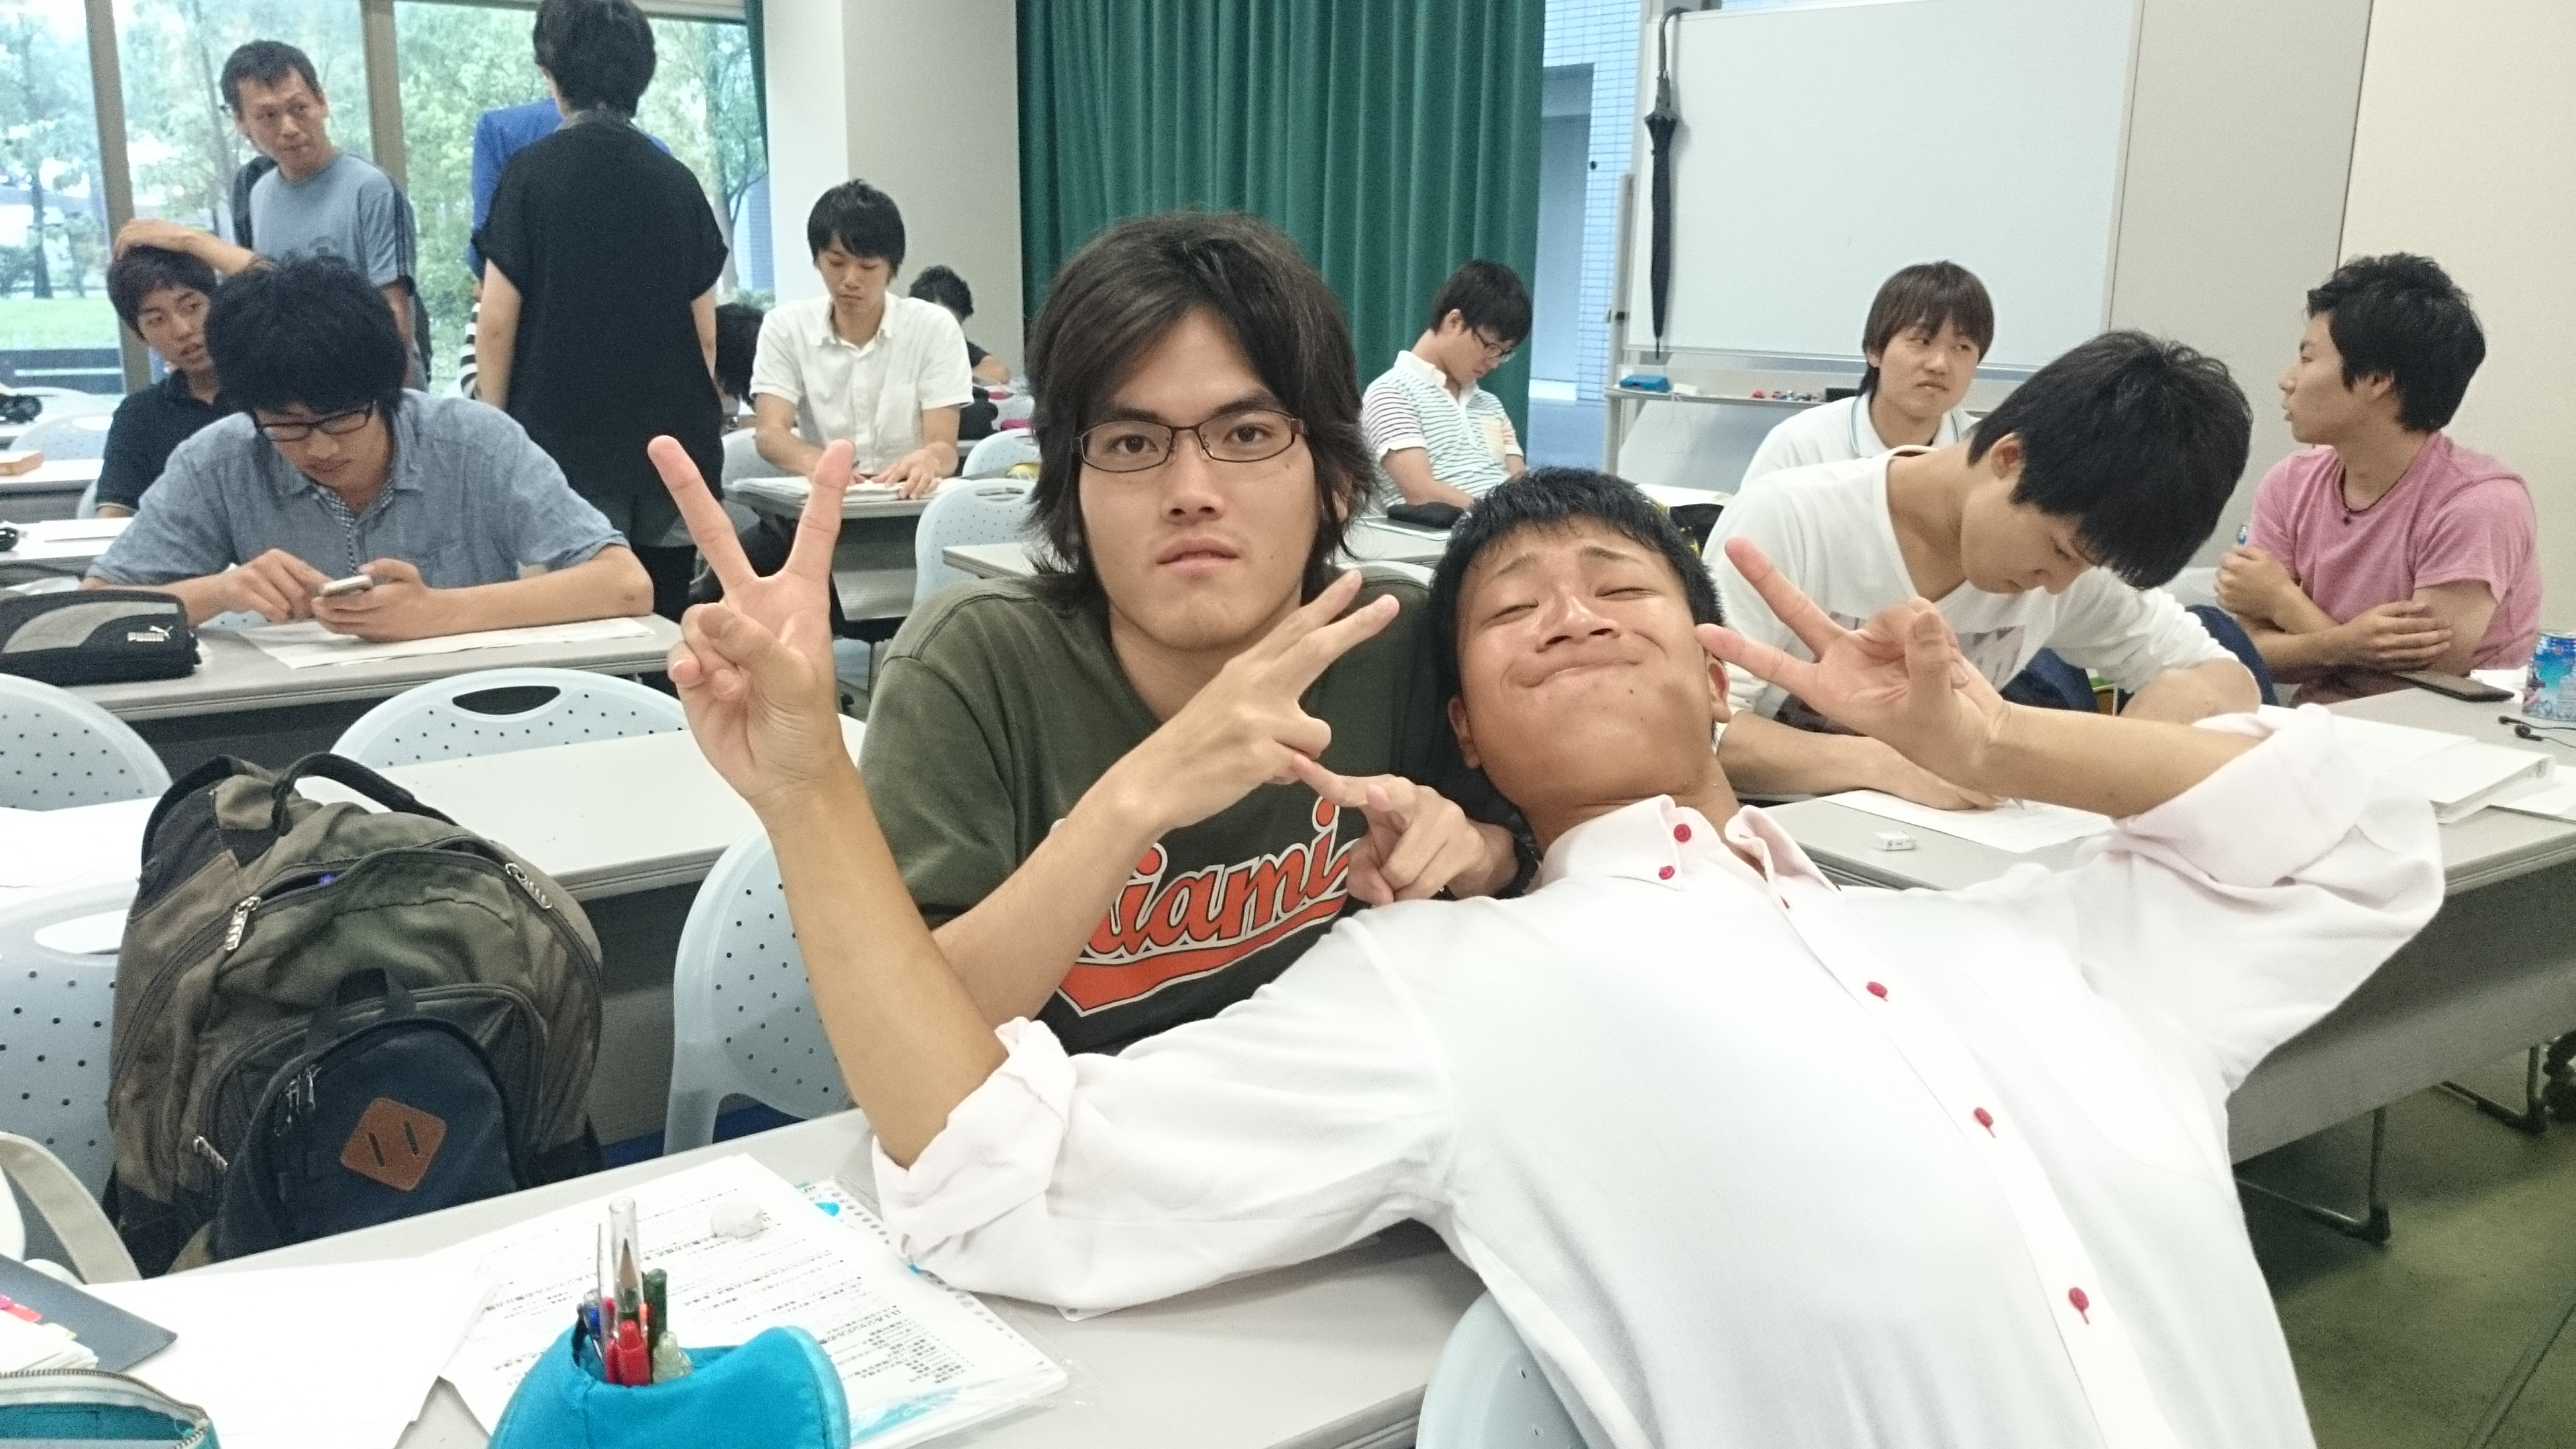
\includegraphics[width=0.8\textwidth]{./section/HigengoUniv/figures/DSC_0388_2}
%\caption{マタヨシ清掃員認定試験会場における、学長と清掃員。}
%\end{figure}
%



%%%%%%%%%%%%%%%%%%%%%%%%%%%%%%%%%%%%%%%%%%%%%%%%%%%%%%%%%
%・非言語大学(タケダ)
%・入学要項、学部、学科、求める学生像、科目数、試験内容、スタッフ一覧
%  ・ポ大学について + 入試問題
% ・非言語大学入試問題について、数学・物理・外国語
%  ・結論:受験生に向けて

%%%% アバポンヌ船長の文化的側面
%-----------------------------------------%
\section{アバポンヌフ船長の文化的側面}
%-----------------------------------------%
\subsection{アボンポンヌ船長}
本研究グループは、アバポンヌ船長に対する研究を進めてきた。
アバポンヌ船長とは、その名の通り「船長」であり、様々な理論から存在が確実視されている船長人間である。
ここで船長人間とは船長でありながら人間である二重性を実現している存在であり、
前期量子力学的には光が粒子性と波動性の二重性を持っていると結論付けられたことの
類推によって理解することが可能となる。
しかし、「アバポンヌ」の部分に関しては様々な理論的予測は未だ乱立した状態にあり、
革新的・統一的な見解は得られていない。
アバポンヌは過去300年間未解明の現象であり、アバポンヌ問題が解けた場合、すべての物理事象を
描像することのできる大アバポンヌ1000元連立300次元方程式を導くことができる。
この超多次元連立方程式は現在のスーパーコンピューターの性能では、人類の有史と同じ程の
計算時間を要するため、アバポンヌ問題を解き連立方程式を導いても結局は何も言っていないのと
同義であるという至極真っ当な意見も多数見受けられる。\par

しかし、本研究グループでは別途スーパーハイパーコンピューターを開発したのでアバポンヌ連立方程式が導けた場合、そこから一般解は1秒で導出できると予測している。
そこで本研究グループでは数あるアバポンヌ理論のうち最も欠陥の少ない、ジェネラルアバポンヌ
理論を参考に解析を進めた。

%------------------------------------------%
\subsubsection{一般的な船長という概念}
%------------------------------------------%
本研究グループはアバポンヌ船長を研究対象にするために、まず一般的な船長という概念についての基礎研究を行った。\par
船長とは、特定の船舶の乗組員で、船舶の指揮者であるとともに船主(船舶所有者)の代理人として、乗組員の監督,船舶・積み荷の管理,運航の指揮などについて、
法律上多くの権限と義務を有している。
つまり船長とはその名の通り「船の長」であり、村長\footnote{アンゴラ村長を除く。}に匹敵する長である。
本研究グループは一般的な船長の持つ権限はアバポンヌ船長にも付与されているとする仮定(ジェネラルアバポンヌ仮定)を採用した。
この仮定はアバポンヌ船長の研究を進めている学会である船長学会において一般的に認知されている論法である。
以下に一般的な船長の有する権利をジェネラルアバポンヌ仮定で解釈を行った結果を列挙する。

\begin{description}
\item[(1)指揮命令権(船員法第7条)]\mbox{}\\
アバポンヌ船長は、理学部内での船長以外の教務委員(海員)を指揮監督し、かつ理学部(以下では船内)にある旅客などに対し、その職務を行うにつき必要な命令をすることができる。
その必要な命令は法律の範疇を超えることができ、軍司令部を掌握し理学部構内に戒厳令を敷くことも可能となり、対アバポンヌ船長の勢力への全面戦争の体勢は整っている。

\item[(2)懲戒権(船員法第22条)]\mbox{}\\
アバポンヌ船長は、船内規律を守らない海員を懲戒することができる。

\item[(3)強制権(船員法第25~28条)]\mbox{}\\
船長は、海員、旅客などが、凶器、爆発又は発火しやすい物、劇薬その他の危険物を所持するときは、その物につき保管、放棄などの必要な処置をすることができる。
つまり4年生実験の総指揮は実はアバポンヌ船長が執っており、何か問題があった場合理学部物理学科、化学科、生物学科、地球惑星学科の各専攻長はアバポンヌ船長への連絡が義務付けられている。
また、船内にある者の生命、身体又は船舶に危害を及ぼすような行為をしようとする海員その他船内にある者に対し、その危害を避けるのに必要な処置をすることができる。
船長は、海員が雇入契約の終了の公認があった後船舶を去らないときは、その海員を強制して船舶を去らせることができる。

\item[(4)行政庁に対する援助の請求(船員法第29条)]\mbox{}\\
船長は、海員・旅客などが人命や船舶に危害を及ぼしたり、船内の秩序を著しくみだすような場合、必要があると認めたときは、行政庁の援助を求めることができる。

\item[(5)司法警察員としての職務(刑事訴訟法第190条など)]\mbox{}
遠洋区域、近海区域又は沿海区域を航行する総トン数20トン以上の船舶の船長は、船内における犯罪につき、司法警察員として、犯罪の捜査、犯人の逮捕などの行為を行う。
つまりアバポンヌ船長は理学部構内の平和を保つための警備員としての仕事も行わなければならない。

\item[(6)船内死亡者に対する処置(船員法第15条)]\mbox{}\\
船長は、船舶の航行中、船内にある者が死亡したときは、命令の定める一定の条件のもとに、これを水葬に付すことができる。
アバポンヌ船長は何度か水葬されている。
\end{description}

アバポンヌ船長は以上に示した、一般的な権限を所有しており、特にアバポンヌ船長にのみ付与されているとされる権限について以下で述べる。
\footnote{ここではジェネラルアバポンヌ仮定に基いた解釈であることに留意し、その他の理論の下では成立しないことも知られており大統一アバポンヌ理論の構築が進められている。}

\begin{description}
\item[(A)日本の伝統権]\mbox{}\\
たとえ同僚が作業に集中していても、その作業を強制的に中断させ便所に連れ出す事ができる。
とくにアバポンヌ船長の持つこの権限は非常に強力であり、そのため権利剥奪を主張する勢力が後を絶たない。
そこでアバポンヌ船長は(2)懲戒権を濫用し、反対勢力を黙らせている。

\item[(B)顔色判定誤認識権]\mbox{}\\
これはジェネラルアバポンヌ仮定におけるアバポンヌ・カオイロ方程式の特解により導き出され、アバポンヌ船長が有しているとされる権限である。
アバポンヌ船長は、その権限の強力さから様々な勢力から命を狙われており、そのため自らの身の安全を守るためにカメラを向けられた時にカオイロ(顔色)を変更する事ができるとされている。
このカオイロは、クォーク模型におけるカラー荷の類推で論じることができる。
アバポンヌ船長はカラー荷B(青色)を持っている状態のみとされるが、この顔色判定誤認識権については\ref{KAO}節で後述する。
\end{description}

%~~~~~~~~~~~~~~~~~~~~~~~~~~~~~~~~~~~~~~~~~%
\subsubsection{アボンポンヌフ船長の顔色誤認識権}\label{KAO}
%~~~~~~~~~~~~~~~~~~~~~~~~~~~~~~~~~~~~~~~~~%
アバポンヌ船長はカラー荷Bを持っており、青色の状態で観測する事ができるとされている。
しかし、実験的には無色の状態のみ観測にかかるとされているので、ジェネラルアバポンヌ仮定を進めると、アバポンヌ船長には本体である青色船長とともに反青色船長の合計2人がいるとされている。ここで各船長の定義を行う。

\begin{description}
\item[青色アバポンヌ船長]\mbox{}\\
議題に上がっている船長は特に指定がなければ、この青色アバポンヌ船長の事を指す。
性格は非常に活発的であり、獰猛。質量は60kg、カラー荷B、電荷$+\frac{10}{3}$。

\item[反青色アバポンヌ船長]\mbox{}\\
近年、新しい理論体系で組み込まれている青色アバポンヌ船長の反物質人間である。
青色アバポンヌ船長と合わせて理論に組み込むことで、実験的に観測することのできる無色のアバポンヌ船長を予言することができる。
質量は60kg、カラー電荷$\overline{\rm{B}}$、電荷0。
\end{description}

\subsection{顔色認識技術の向上}
アバポンヌ船長は、自らのプライバシーを死守するために顔色を変える。
その顔色を

%===============%
\subsection{文化的側面}
%===============%
本研究グループは以上のアバポンヌ船長の仮定の元に、アバポンヌ船長の文化的側面の研究を進めた。

%-------------------------------------------------%
\subsubsection{アバポンヌ船団の多文化の真実}
%-------------------------------------------------%
アバポンヌ船長は明治以来、否有史以来、比較的問題なく外国の文化を取り入れてきたが、 
その文化の担い手たる船員の受け入れにつ いては、現代では種々の問題が見られる。 
ことに最近20年ほどは外 国籍を持つ船員が船長率いる軍団に在住するようになってきた。 
総務省統計局によると2000年現在でアバポンヌ船団に在住する外国籍船員は約1311000人で 、
総人口の 1.03\%となっ てい る。 
これは1995年以来14.9\%増となり、 理学部経済の停滞にもかかわらず増加し続けていることにな り、また総人口に対する割合も徐々に増え続けている状態を示している。 
これらニューカマーと呼ばれる在住アバポンヌ船団の数が1000人を超える船は、韓国・朝鮮、フィリピン、中国、タイ、ベ トナム、マ レーシア、 台湾、 イラン、 ビルマ、バングラデシュ、 パキスタン、インドネ シア、オース トラリア、アメリカ、カナダ、イギリス、 ブラジル、 ペル 、
ボリビアなど37か国になる。 
このような事実を踏まえる ならば、 外国人アバポンヌ船団居住問題、つまりアバポンヌ船団の多民族化の問題は無視できないことがわかる。 

%--------------------------------------------%
\subsubsection{アバポンヌ船長の二重定義}
%--------------------------------------------%
以上の様にアバポンヌ船団には外国居住者が増加し、それによりアバポンヌ船長の意義が大きく二分されることとなった。近年の研究ではこの二重定義は「アバポンヌ船長」と「アバポンヌフ船長」として知られている。

%---------------------------%
\subsection{アバポンヌフ船長}
%---------------------------%
アバポンヌフ船長とは一種の環境建築であり、これを紐解くには環境心理学の観点から研究を進める必要があった。
博士課程在席時に行った街路景観の評価構造研究は、評価に個人差があるケースの存在を示している。
街並みは半公共財であるという考え方は、日本においても市民権を得つつあるようだが、個人差がある場合には、それをどう処理するかという問題が出てくる。
博士論文では、総合評価「好ましさ」を「落ち着き・まとまり」と「明るさ・面白み」の2軸に分離することができ、この構造は比較的均質であるのに対し、
どの景観で落ち着きを感じるのか、面白みを感じるのかというところには個人差が存在するという結果が得られている。
したがって、評価の構造にはある程度の共通性を仮定してもいいが、景観の特徴と印象の関連には個人差が存在すると考えられる。
この個人差は、意味と大きく関わっていると考える。
A. Rapoportは「The Meaning of the Environment」の中で、意味の重要性を再三再四指摘しているが、本研究グループの博士論文においても、総合評価の個人差が大きい景観は、解釈の二面性を持っていることを示唆する結果が得られている。つまり、2つの意味に解釈できるため、そうでない景観より個人差が大きかったと考えられるのである。
このように、本研究グループの視点は評価と関わっており、そこには平均的な評価だけでなく評価の個人差も説明したいという意識が根底にはあった。
したがって、本研究グループの文化に対する問題意識の主要なものの一つは、評価を説明する文化、評価の個人差を説明する文化というところにある。

%-----------------------------------------------------%
\subsubsection{アバポンヌフ船長の文化と理由付け}
%-----------------------------------------------------%
「常識の世界地図」という文庫本には、文化の相違を示す様々な事例が掲載されているが、同じ行為・同じ物事が別の意味に取られるという事例のオンパレードといった印象がある。「四」は「死」と同じ発音だから、縁起が悪いという、日本や中国の一部にある迷信は、このような事例の一つである。
当然の事ながら、four, quatre, vierなどの語に、このような縁起の悪さが付きまとうわけではない。
体を清潔にする浴室と不浄な場所の代表であるトイレが一つの部屋に配される西洋型ホテルのバス・ルームは、日本人には理解しづらい例であるが、
この本によると体から出る汚れを水で処理する場所という位置づけだというのが、一緒にする理由だそうだ。
それに対し、日本では共同浴場が一般的であったし、汲み取りの伝統が公共事業として受け継がれたため、トイレと風呂は別々となったのだろうという。
このように、現在文化として定着しているものの中には、普及し始めたときの事情が絡んでいるものも多い。
そして、その成立事情がわかると、それまでよりは違和感が和らぐことが多い。
このように、事情がわかれば理解可能ということも、認識構造には共通性があるが、実際の反応は異なるという事例と捉えることが可能なように思う。
そこで、文化を捉える視点として、「人間の認識の構造には共通性があるが、要素の結びつき方が変わるため、反応は異なることがある。」というメタ理論を設定するというのはどうだろうか。(これは、臨床認知心理学者G.ケリーのパーソナル・コンストラクト理論に近い仮定である。)
これは、評価や認知や反応が異なる事例があれば、なぜそれらが異なるのかを説明するという作業を行い、
人々がある程度納得できる説明を用意するということを文化を扱う研究者の使命の第一としようということである。そのようなやり方でうまく説明できない事例がいくつか出現した際には、仮説を修正することになるが、このようなメタ仮説を明確に呈示しておくことが、
新たな理論の構築を促すためにも必要だと考える。

\newpage

%%%% タウンワーク
%~~~~~~~~~~~~~~~~%
\chapter{TownWorkの旅}
%~~~~~~~~~~~~~~~~
学生たるものバイトをして生活費を稼ぐ必要がある。
その中でも特にバイト学研究の第一人者であるタケダ氏は、これまでに様々なバイトを経験してきたこともあり、
世の中にどのようなバイトが存在しているかに非常に興味をもっていた。
そのため、神戸大学工学部セブンイレブンに入店する度にフリーペーパーであるタウンワークを持ち帰り、熱心な研究を行ってきた。
週刊誌であるタウンワークはタケダ氏にとって、週の初めのこの上ない楽しみになっていた。
毎週、研究室のデスクの上にタウンワークの新刊が積まれていく度にいつしか、タウンワークを収集することが目的となってきたようであり、
そこでタケダ氏は発想の転換からとある研究を思いついたのである。
それは現在まで続く、世界中のバイト戦士のための研究であり、タケダ氏を世界的に有名にした実験である。
その名も「TownWorkの旅」と呼ばれる、各地方の就業率とバイト募集に関する相関を論ずることのできる唯一の手法を思いついたのだ。
\par
本章では、タケダ氏がプロジェクトリーダーである「TownWorkの旅」実験に関する報告を行う。
タウンワークが発行されている県と発行されていない県も存在し、発行されていない県についてはタウンワークと同等の公平性・正確性を持っている雑誌を参考とした。
以下に現在(2018年3月27日)までに取得できた統計情報を示し、それらから予測される就業率を論ずる。
今後はさらに出張を重ね、統計量を増やし統計誤差は削減されると期待される。

%===========================%
\section{現在までに取得できた統計情報}
%===========================%
今回の統計情報を集計するにあたり、制覇した県を検出するための基板設計も行った。
この新検出器板開発に際してCERNの各偉人たちの協力のもと設計・開発を行う予定であったが、
都合が合わず、そこで非言語大学独自の技術を用いた検出器板となった。
これら新しく制覇された県を検出することのできるTownWorkの旅検出器板(TW-Board)を図\ref{fig:TWBoard}に示す。
また現在までに制覇することのできた日本全国地図の最新版を図\ref{fig:JapanMap}に示す(2019年1月20日現在)。

\begin{figure}
\centering
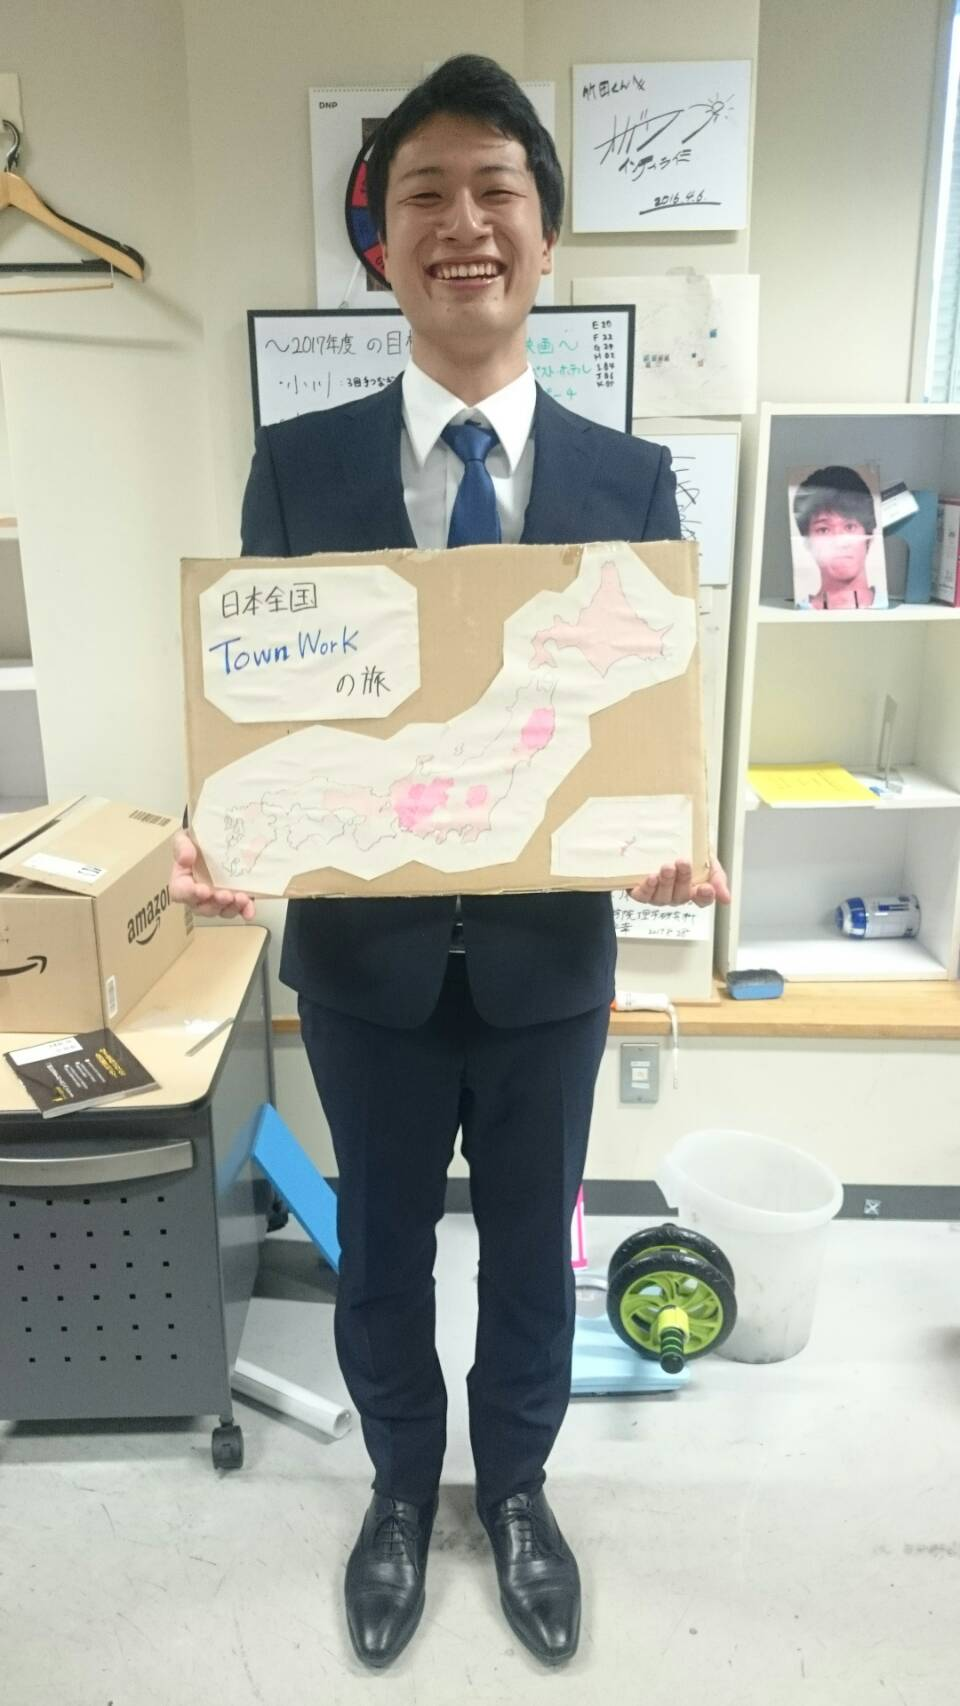
\includegraphics[scale=0.2]{TWBoard.jpg}
\caption{新検出器板を持ち、満面の笑みを浮かべるオマンガン伯爵。壁には山元大生、オガワインティライミのサイン等の懐かしのアイテムが転がっている。}
\label{fig:TWBoard}
\end{figure}


\begin{figure}
  \centering
  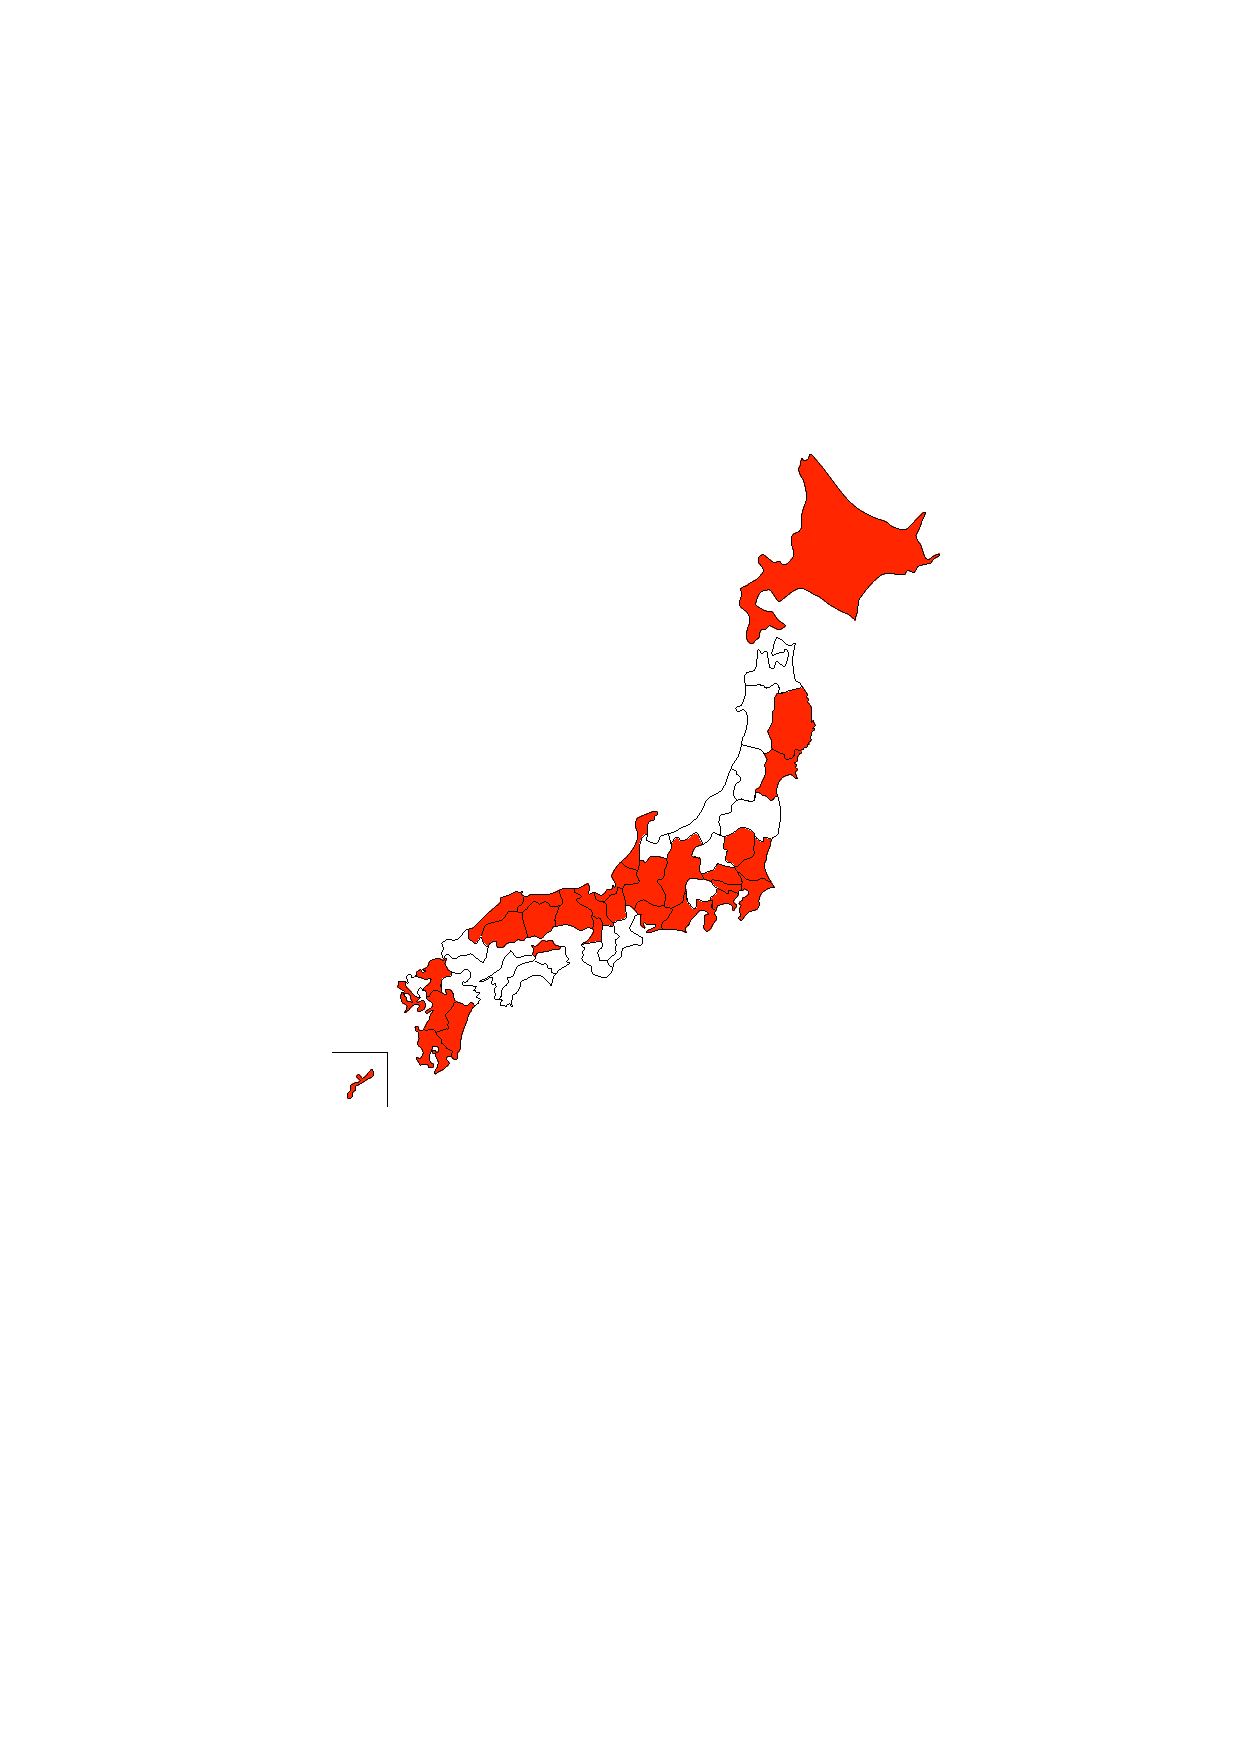
\includegraphics[width=0.9\textwidth]{./section/TownWork/figures/JapanMap.pdf}
  \caption{赤色で示された領域が、現在までにタウンワーク制覇することのできた都道府県である。北から順に、北海道、岩手県、宮城県、群馬県、茨城県、千葉県、東京都、埼玉県、長野県、岐阜県、静岡県、愛知県、
  石川県、福井県、滋賀県、京都府、大阪府、兵庫県、岡山県、島根県、鳥取県、広島県、山口県、香川県、福岡県、宮崎県、長崎県、熊本県、鹿児島県、沖縄県の計30県を制覇することができている。
  残りの17県の早急な制覇が望まれるところである。}
  \label{fig:JapanMap}
\end{figure}


\begin{figure}[htbp]
    \centering
  \begin{minipage}{0.4\linewidth}
    \centering
    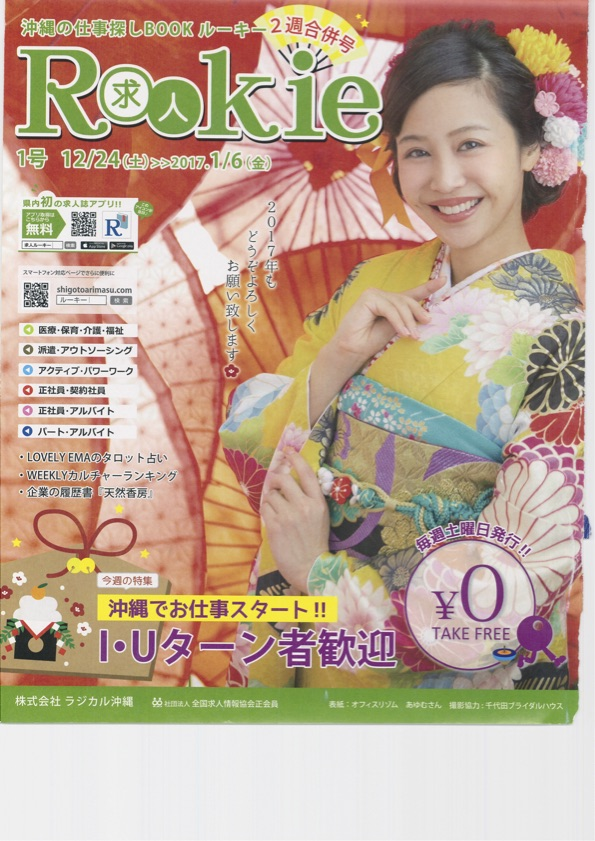
\includegraphics[scale=0.2]{tw.jpg}
  \end{minipage}
  \begin{minipage}{0.4\linewidth}
    \centering
    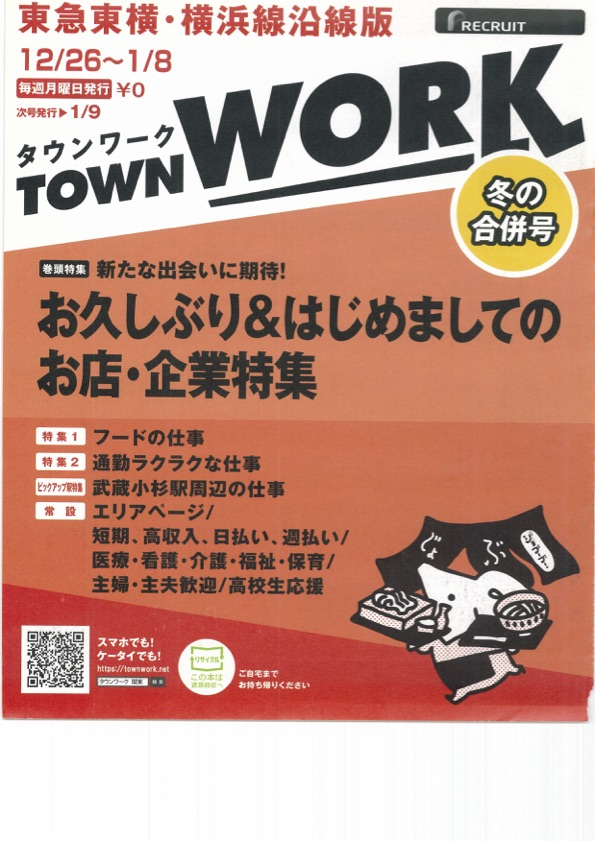
\includegraphics[scale=0.2]{tw1.jpg}
  \end{minipage}\\
  \begin{minipage}{0.4\linewidth}
    \centering
    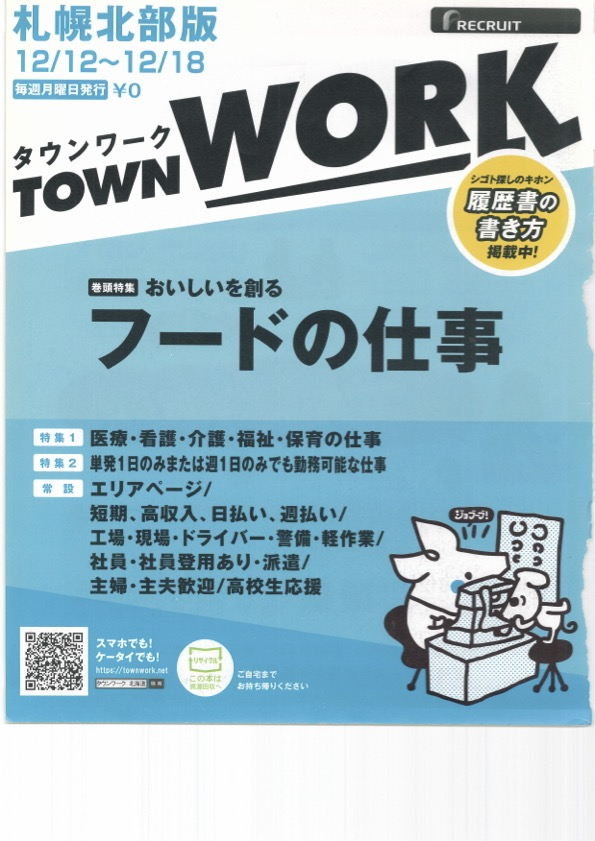
\includegraphics[scale=0.2]{tw2.jpg}
  \end{minipage}
  \begin{minipage}{0.4\linewidth}
    \centering
    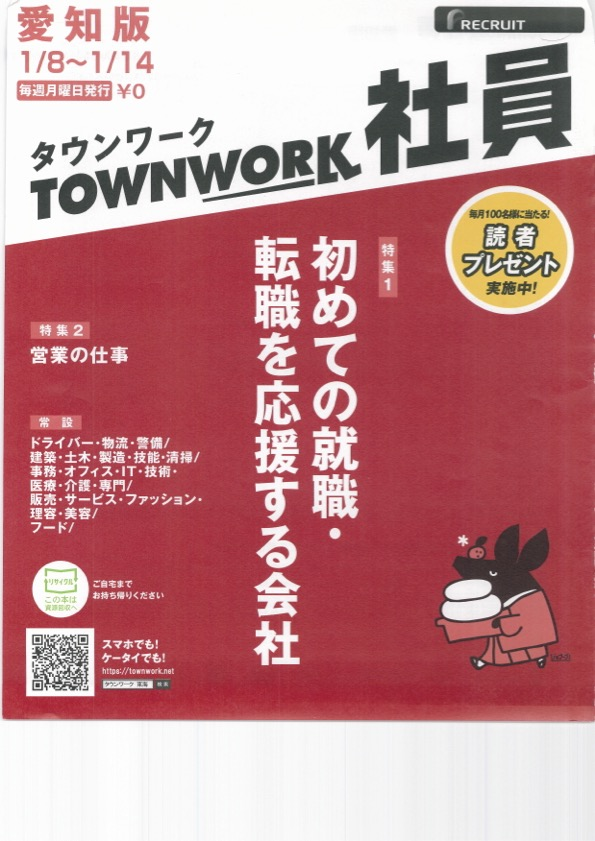
\includegraphics[scale=0.2]{tw3.jpg}
  \end{minipage}
  \begin{minipage}{0.4\linewidth}
    \centering
    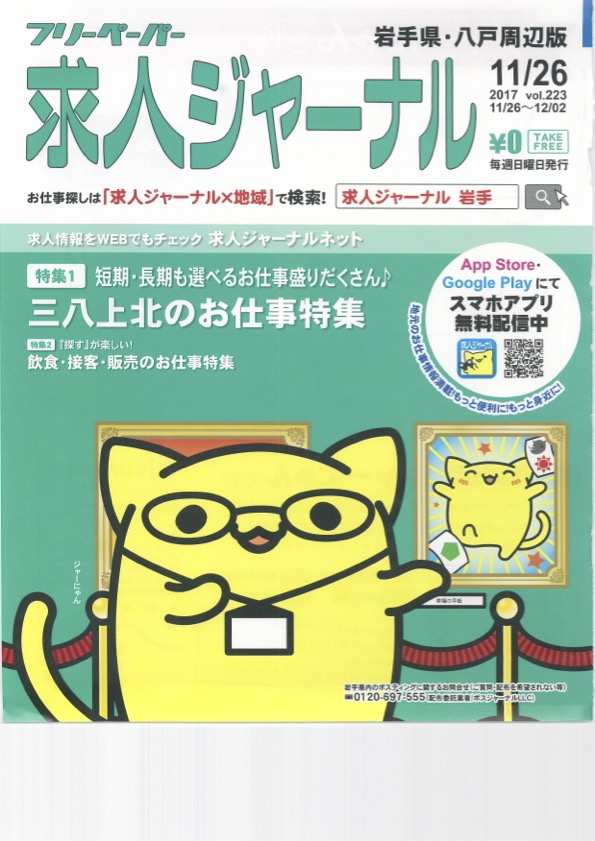
\includegraphics[scale=0.2]{tw4.jpg}
  \end{minipage}
  \begin{minipage}{0.4\linewidth}
    \centering
    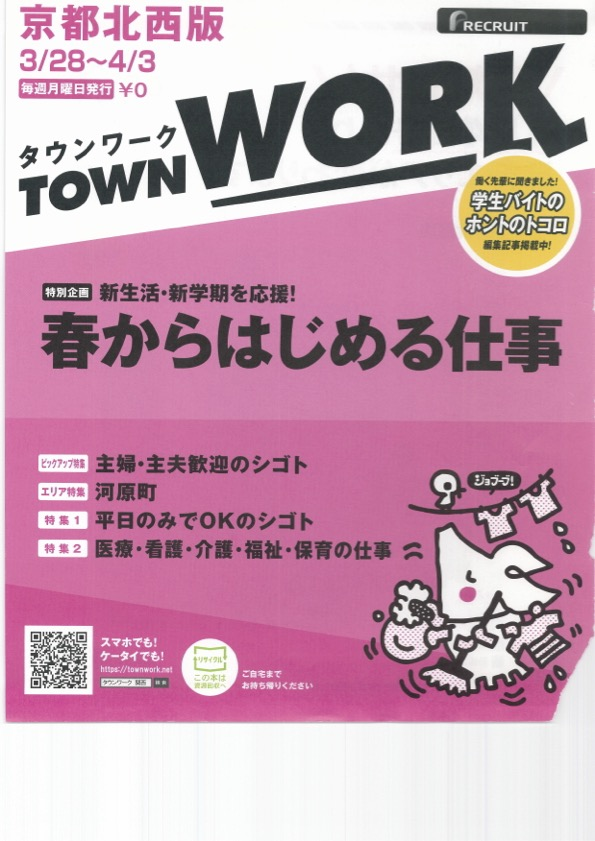
\includegraphics[scale=0.2]{tw5.jpg}
  \end{minipage}
  \caption{TownWorkの旅で手に入れた各地方の表紙一覧。}
  \label{CscDetaDphi-CSide}
\end{figure}

\newpage
\begin{figure}[htbp]
    \centering
  \begin{minipage}{0.4\linewidth}
    \centering
    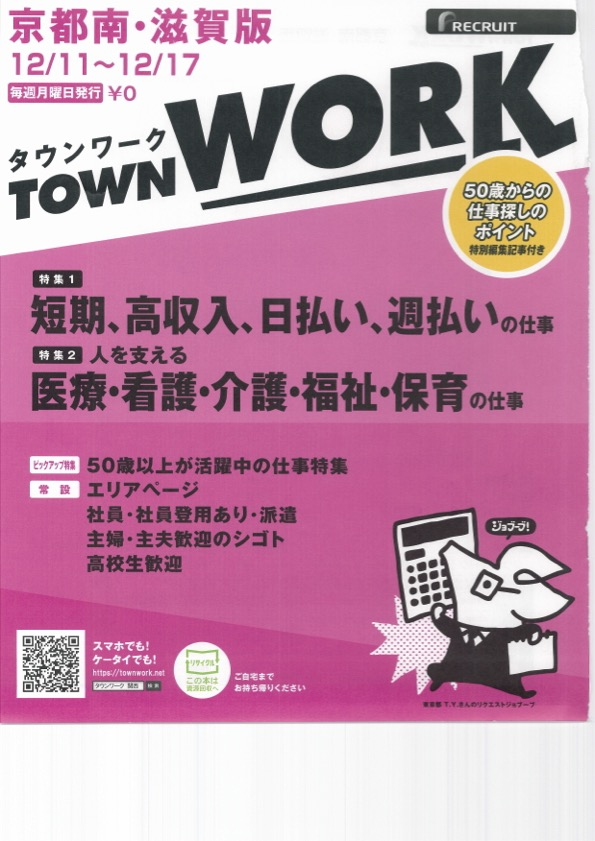
\includegraphics[scale=0.2]{tw6.jpg}
  \end{minipage}
  \begin{minipage}{0.4\linewidth}
    \centering
    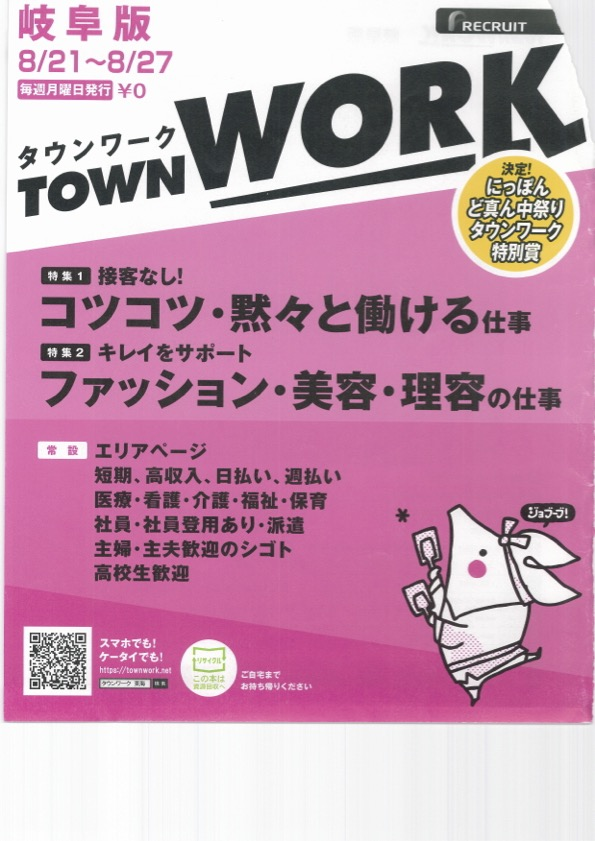
\includegraphics[scale=0.2]{tw7.jpg}
  \end{minipage}\\
  \begin{minipage}{0.4\linewidth}
    \centering
    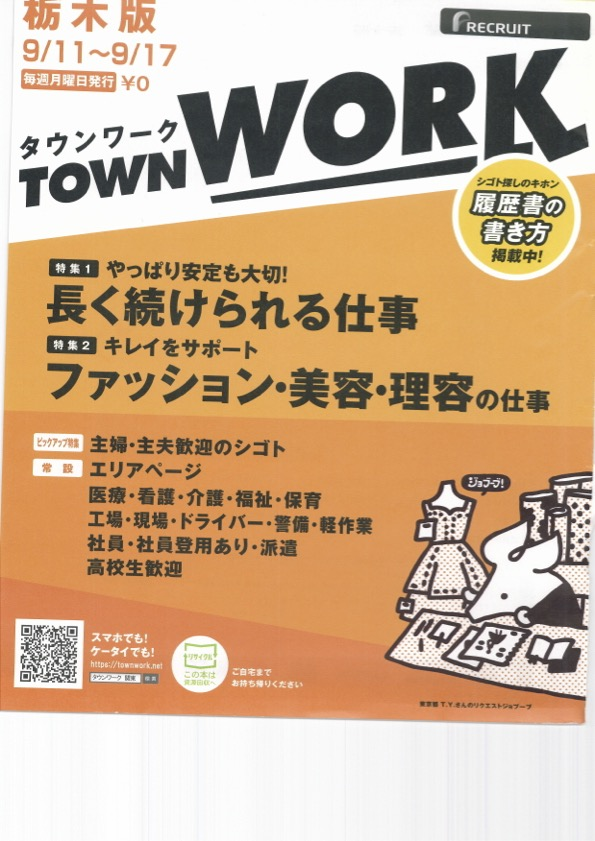
\includegraphics[scale=0.2]{tw8.jpg}
  \end{minipage}
  \begin{minipage}{0.4\linewidth}
    \centering
    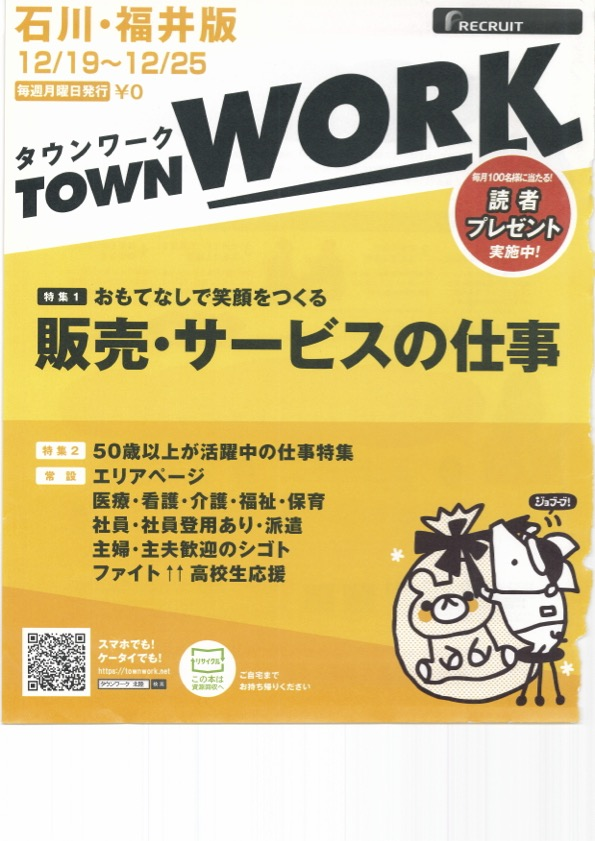
\includegraphics[scale=0.2]{tw9.jpg}
  \end{minipage}
  \begin{minipage}{0.4\linewidth}
    \centering
    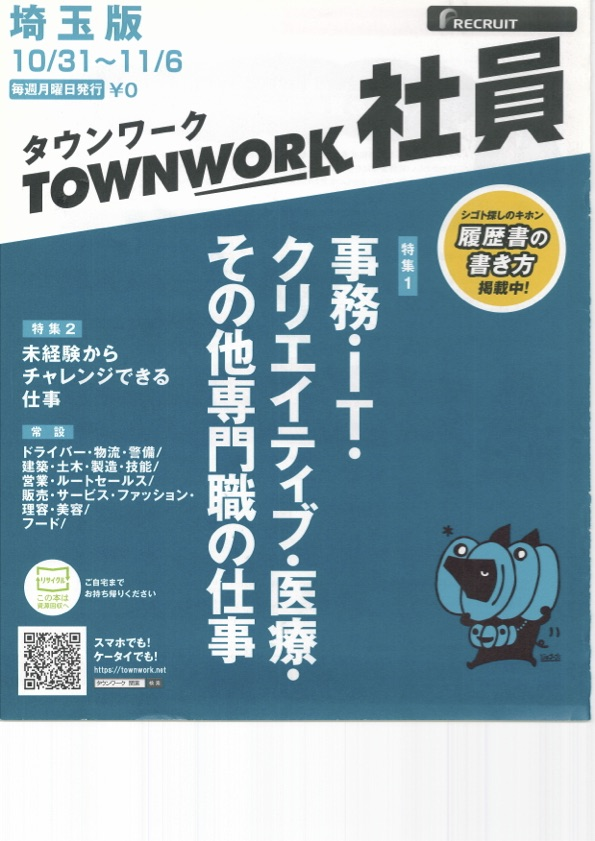
\includegraphics[scale=0.2]{tw10.jpg}
  \end{minipage}
  \begin{minipage}{0.4\linewidth}
    \centering
    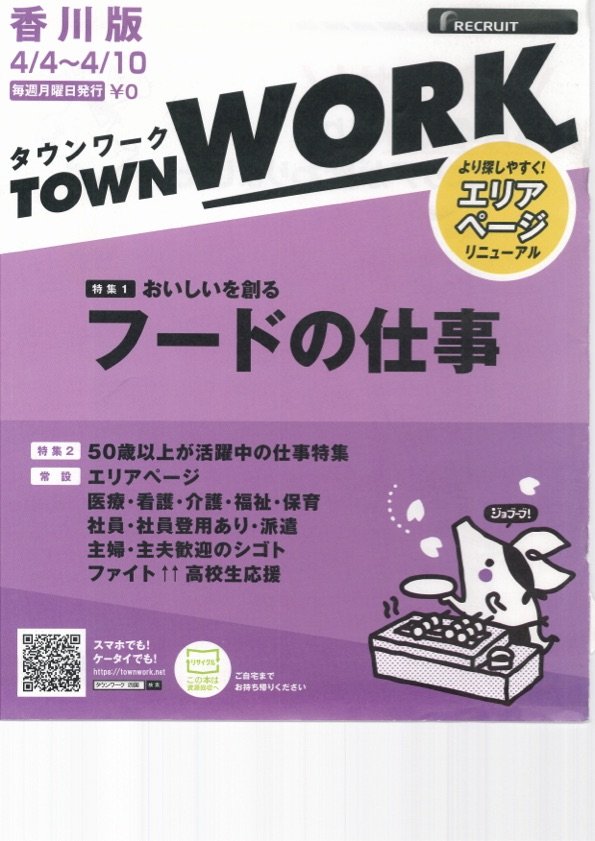
\includegraphics[scale=0.2]{tw11.jpg}
  \end{minipage}
  \caption{TownWorkの旅で手に入れた各地方の表紙一覧。}
  \label{CscDetaDphi-CSide}
\end{figure}

\newpage
\begin{figure}[htbp]
    \centering
  \begin{minipage}{0.4\linewidth}
    \centering
    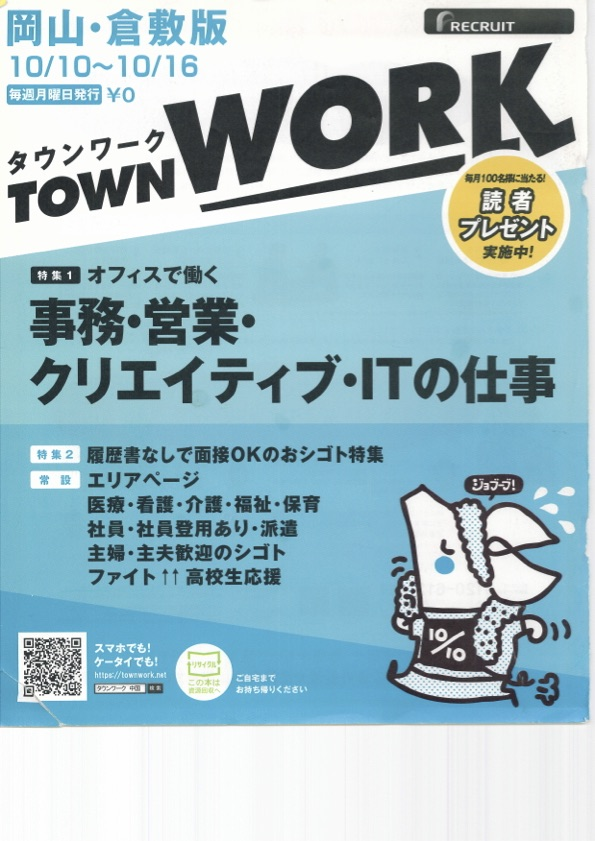
\includegraphics[scale=0.2]{tw12.jpg}
  \end{minipage}
  \begin{minipage}{0.4\linewidth}
    \centering
    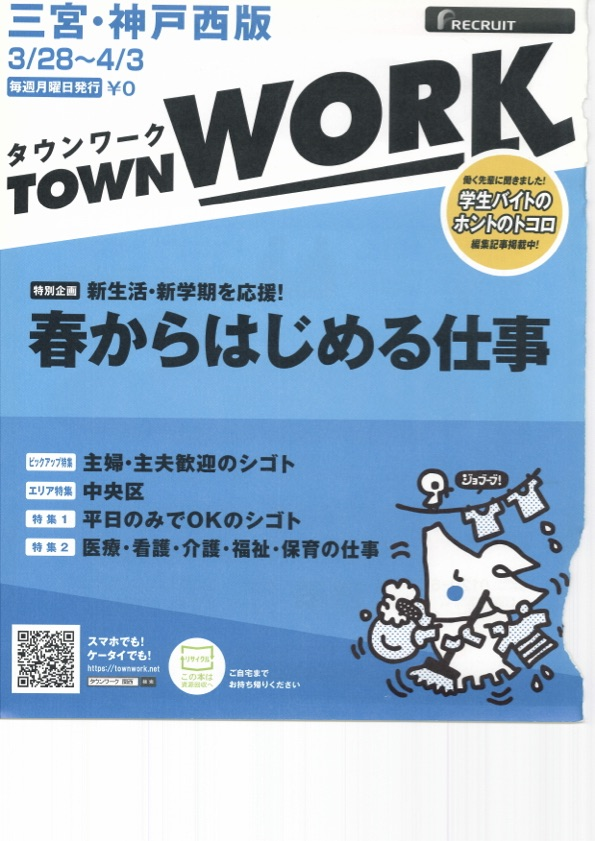
\includegraphics[scale=0.2]{tw13.jpg}
  \end{minipage}\\
  \begin{minipage}{0.4\linewidth}
    \centering
    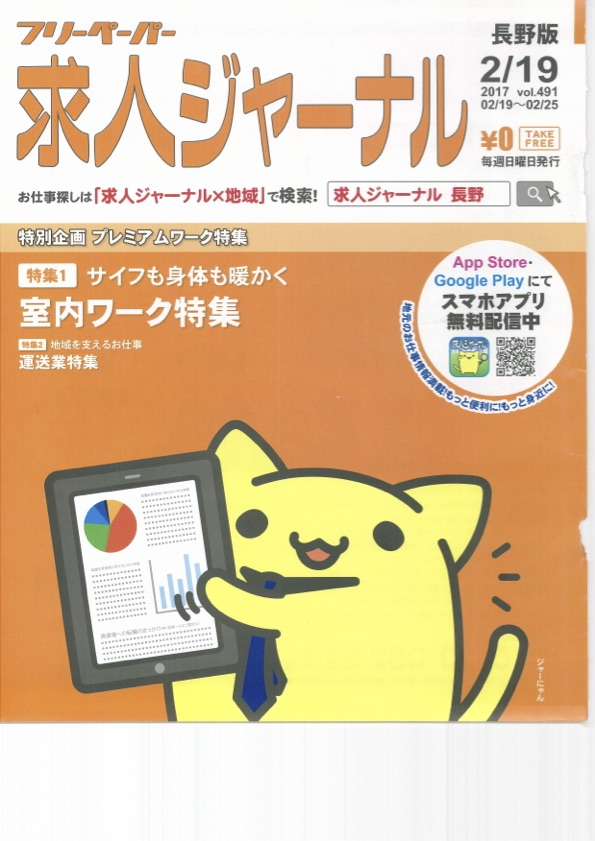
\includegraphics[scale=0.2]{tw14.jpg}
  \end{minipage}
  \begin{minipage}{0.4\linewidth}
    \centering
    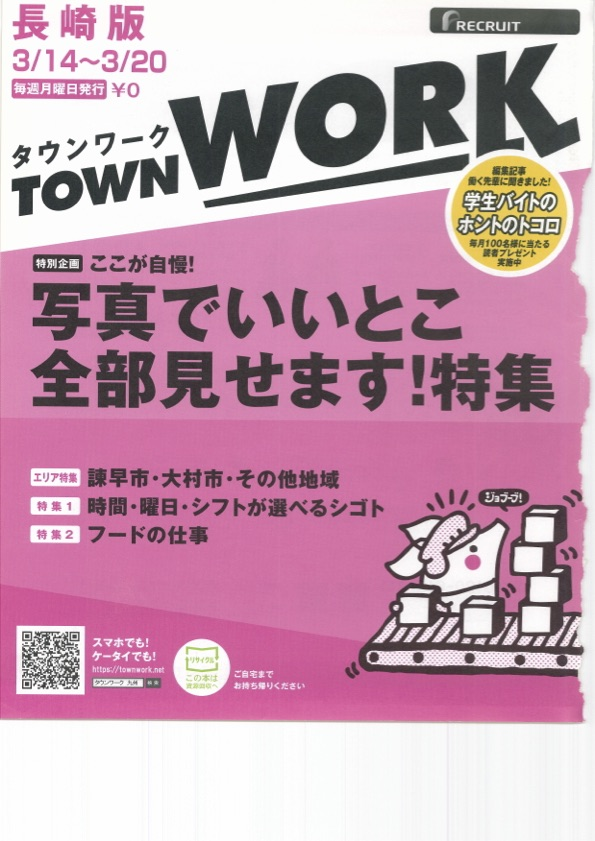
\includegraphics[scale=0.2]{tw15.jpg}
  \end{minipage}
  \begin{minipage}{0.4\linewidth}
    \centering
    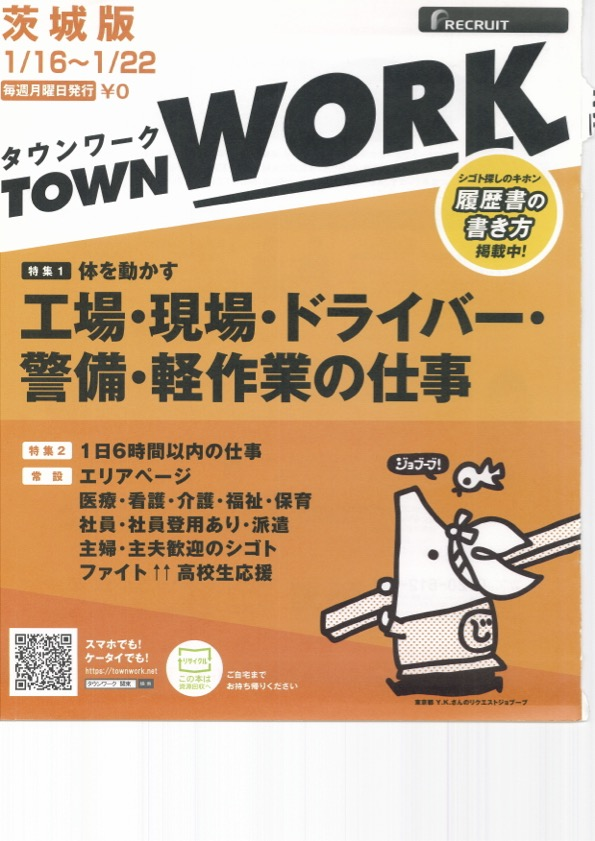
\includegraphics[scale=0.2]{tw16.jpg}
  \end{minipage}
  \begin{minipage}{0.4\linewidth}
    \centering
    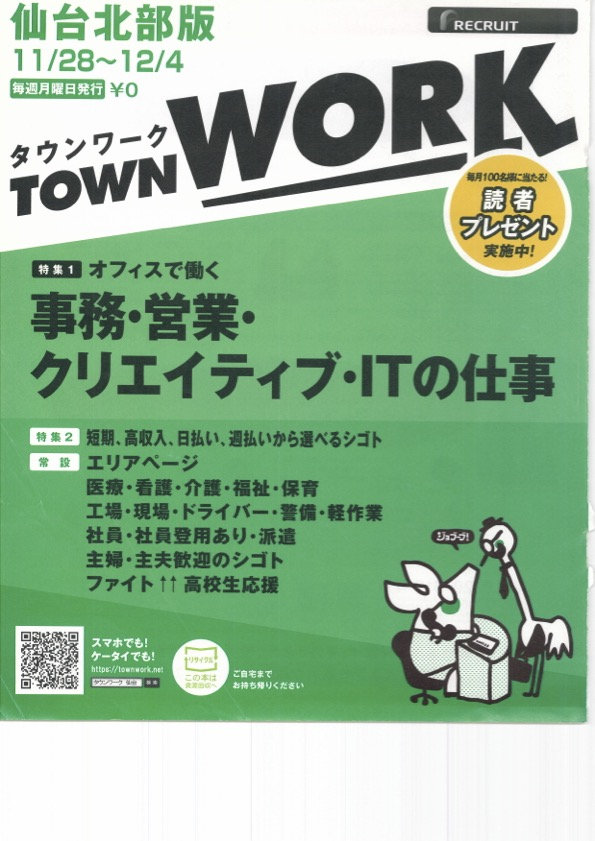
\includegraphics[scale=0.2]{tw17.jpg}
  \end{minipage}
  \caption{TownWorkの旅で手に入れた各地方の表紙一覧。}
  \label{CscDetaDphi-CSide}
\end{figure}

\newpage
\begin{figure}[htbp]
    \centering
  \begin{minipage}{0.4\linewidth}
    \centering
    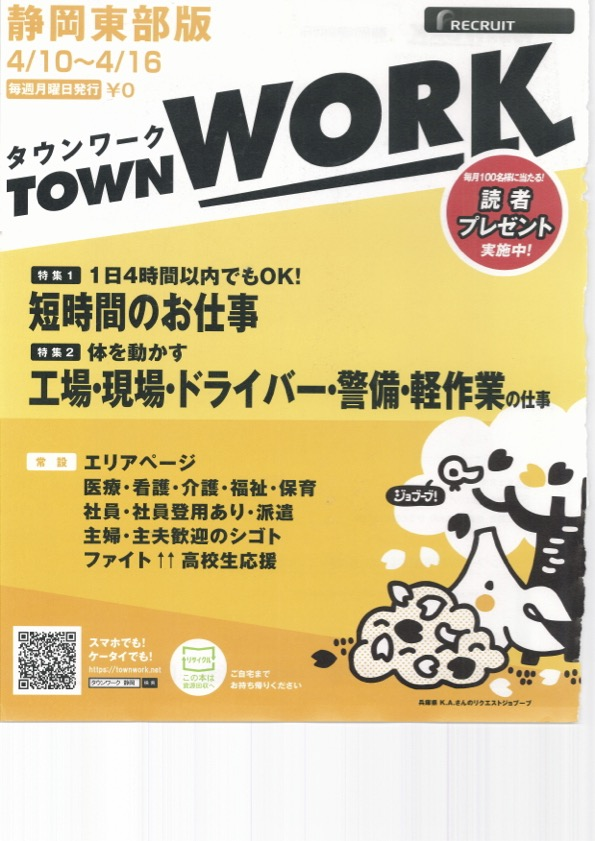
\includegraphics[scale=0.2]{tw18.jpg}
  \end{minipage}
  \begin{minipage}{0.4\linewidth}
    \centering
    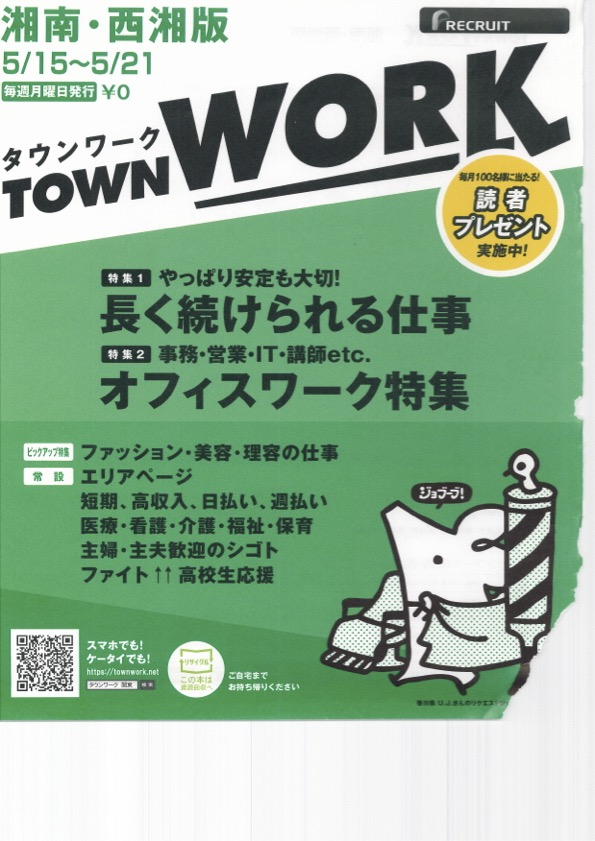
\includegraphics[scale=0.2]{tw19.jpg}
  \end{minipage}\\
  \begin{minipage}{0.4\linewidth}
    \centering
    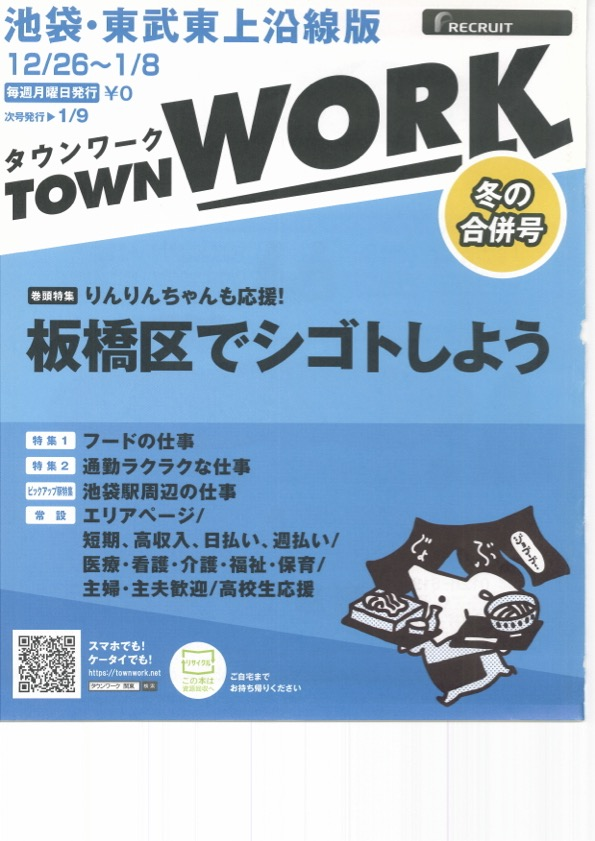
\includegraphics[scale=0.2]{tw20.jpg}
  \end{minipage}
  \begin{minipage}{0.4\linewidth}
    \centering
    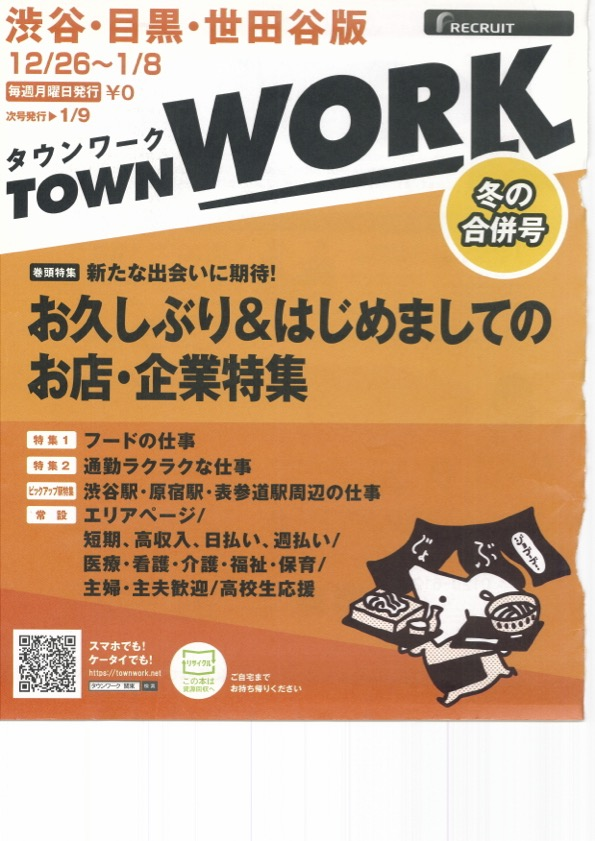
\includegraphics[scale=0.2]{tw21.jpg}
  \end{minipage}
  \begin{minipage}{0.4\linewidth}
    \centering
    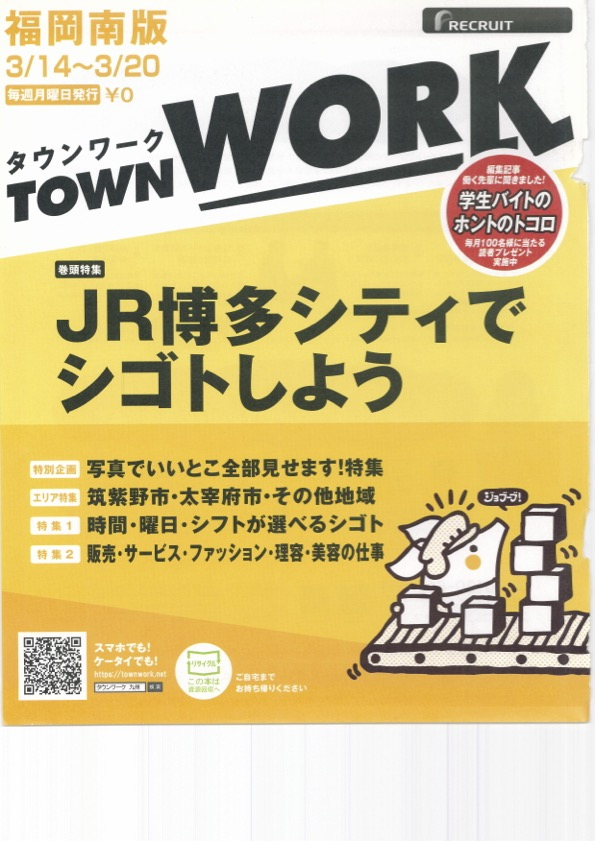
\includegraphics[scale=0.2]{tw22.jpg}
  \end{minipage}
  \caption{TownWorkの旅で手に入れた各地方の表紙一覧。}
  \label{CscDetaDphi-CSide}
\end{figure}

\newpage
\clearpage
\newpage
\clearpage

%%% 食事という概念
%!TEX root = ../../main.tex
\chapter{食事という概念}
日本の食文化の大切さについては誰しも異論がないが、ではその内容はなにかと尋ねられると、答えは曖昧きわまりない。
正しい日本食文化の海外展開が急がれ、次世代へよき食文化の伝統を伝えるべきときに、その内容が明確でないことは重大な欠陥といわなくてはならない。
そこで、まず共通理解としての日本食文化の概念を構築する必要がある。
(2)日本食文化の範囲
食文化の範囲は広い。生産、食材、調理はもちろん、嗜好と栄養、食事行動、食べる道具と場など、食に関するすべての文化を含む人類共通の概念である。
そのなかで日本の食文化といったとき、日本の歴史と環境からうみだされた特徴があらわれる。
例えば、片刃の包丁という日本独特の道具に代表されるような日本料理の技術、目で食べさせるといわれる盛りつけと和食器の繊細な美、しつらいともてなしの心、うまみという味わいに代表される日本人の淡薄ななかに深味を求める嗜好、手を加えない素材の味わいとそれをひきたてる熟成された発酵調味料、豊かな海と地味から生み出される独自の食材など、そこには他の食文化とはっきりと一線を画した日本の食文化の領域がある。

現代は飽食の時代とも呼ばれており、食事をすること一つ取っても非常に多用な食事様式が存在しており、豊かな時代である。


%%%%%%%%%%%%%%%%%%%%%%%%%%%%%%%
\section{50\%藏重久弥}
%%%%%%%%%%%%%%%%%%%%%%%%%%%%%%%
世界には自分と同じ姿の人間が3人いるという迷信は、一度は耳にしたことがあるだろう。
これをドッペルゲンガーと呼び、本人同士が直接的に会うとビックバンが生ずるとも言われている。
このように、容姿が大変似ている人というのは、近年のものまねブームを鑑みても分かるように、一定数はいるのである。
これらは所詮は「似ている」の範疇を出ないのであって、本人ではない。
しかし、近年50\%の純度で藏重久弥と全く同じである人物が発見された。
LANSBOXで働いていらっしゃる重久さんである。
一目瞭然、純度50\%の神戸大学教授である。
写真からも読み取れるように、先祖代々50\%藏重久弥を名乗って脈々と受け継がれてきたその生命のリレーの、現在の走者である重久のお写真を図\ref{Fig:Shigehisa}に示す。
ここからも分かるように、アキラ100\%は所詮おぼん芸人であり、決して100\%藏重久弥ではない。
この重久さんこそが50\%藏重久弥である。
名札からは姓しか分からないが、もし名前が「藏弥」であれば、この重久さんこそが藏重100\%となるのであろうが、名前については現在確認中である。
% ----------------------------------------
\begin{figure}[h]
\centering
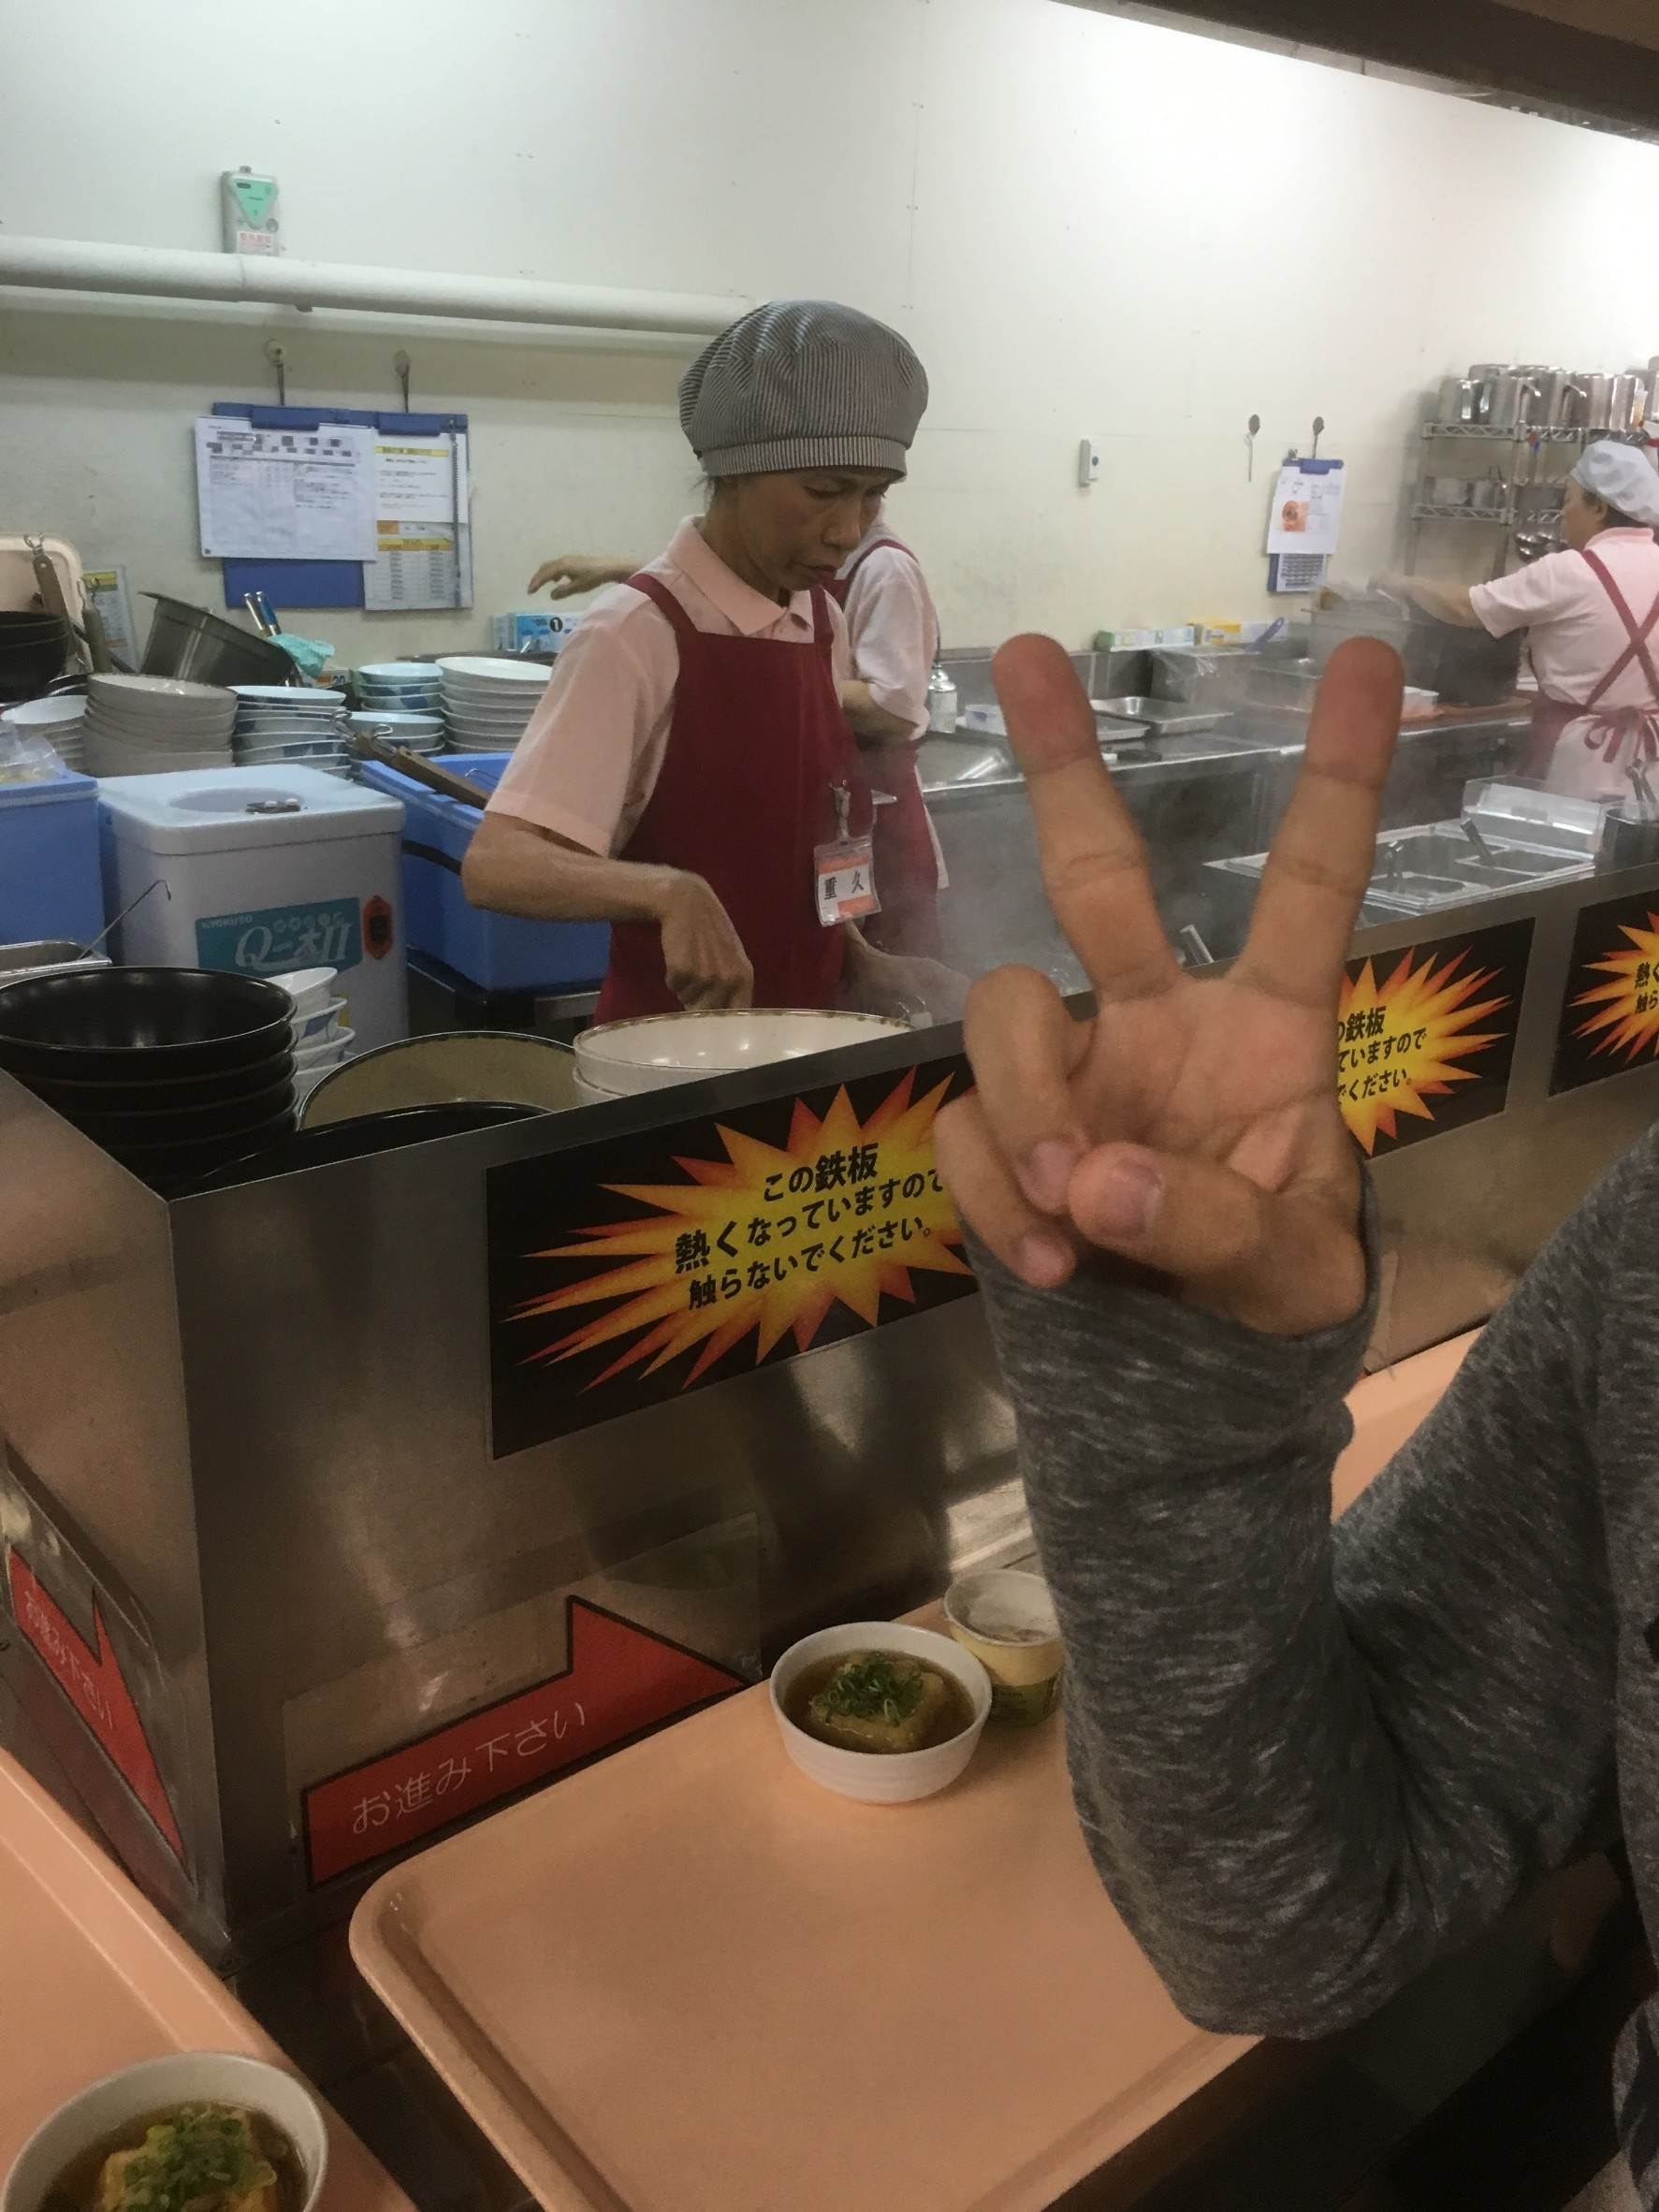
\includegraphics[width=0.5\textwidth]{./section/Shokuji/figures/Shigehisa.jpg}
\caption{LANS Boxで毎日給仕していただいている重久さん。}
\label{Fig:Shigehisa}
\end{figure}
% ----------------------------------------



%%%%%%%%%%%%%%%%%%%%%%%%%%%%%%%
\section{蕎麦は二度美味しい}
%%%%%%%%%%%%%%%%%%%%%%%%%%%%%%%
蕎麦派か、うどん派か。これは議論の分かれる所であり、食べ方や出汁のとり方から何から何まで全く違う日本の誇るべき食べ物である。
俗に関東は蕎麦文化、関西はうどん文化として知られており、時代劇等でも江戸っ子の粋な食べ物として、蕎麦が登場するくらいである。
このように蕎麦は、粋な、いなせな食べ物としてのイメージが定着しており、特に食べ方として次のような作法を取ることが一般的であろう。
\begin{enumerate}
\item つゆに付けず、そのまま味わう
\item 次につゆに付けて、ツルッと味わう
\end{enumerate}
という、いわゆる二度味わうというのが一般的に知られている作法である。
しかし、近年、とある学者が次次に示す、新しい蕎麦の食べ方を考案し、話題になっている。
\begin{enumerate}
\item まず、自分の好みの食べ方で蕎麦を食べきる。
\item 次に、嘔吐する。そうすることで蕎麦が食道を二回通り、同じ値段で蕎麦を二度味わうことができる。
\end{enumerate}
これは非常に画期的な学説であり、+100円で大盛りにするよりも経済的効果も見込める。
たった1200円で、信州そばを二度味わうことができるのである。
しかし、この新手法を用いるには、現在の科学具術では、図\ref{Fig:Soba}に示すように、その副作用が非常に大きく、いかにして簡単に手軽に二度味わうかが次の課題と言えよう。

% ----------------------------------------
\begin{figure}[h]
\centering
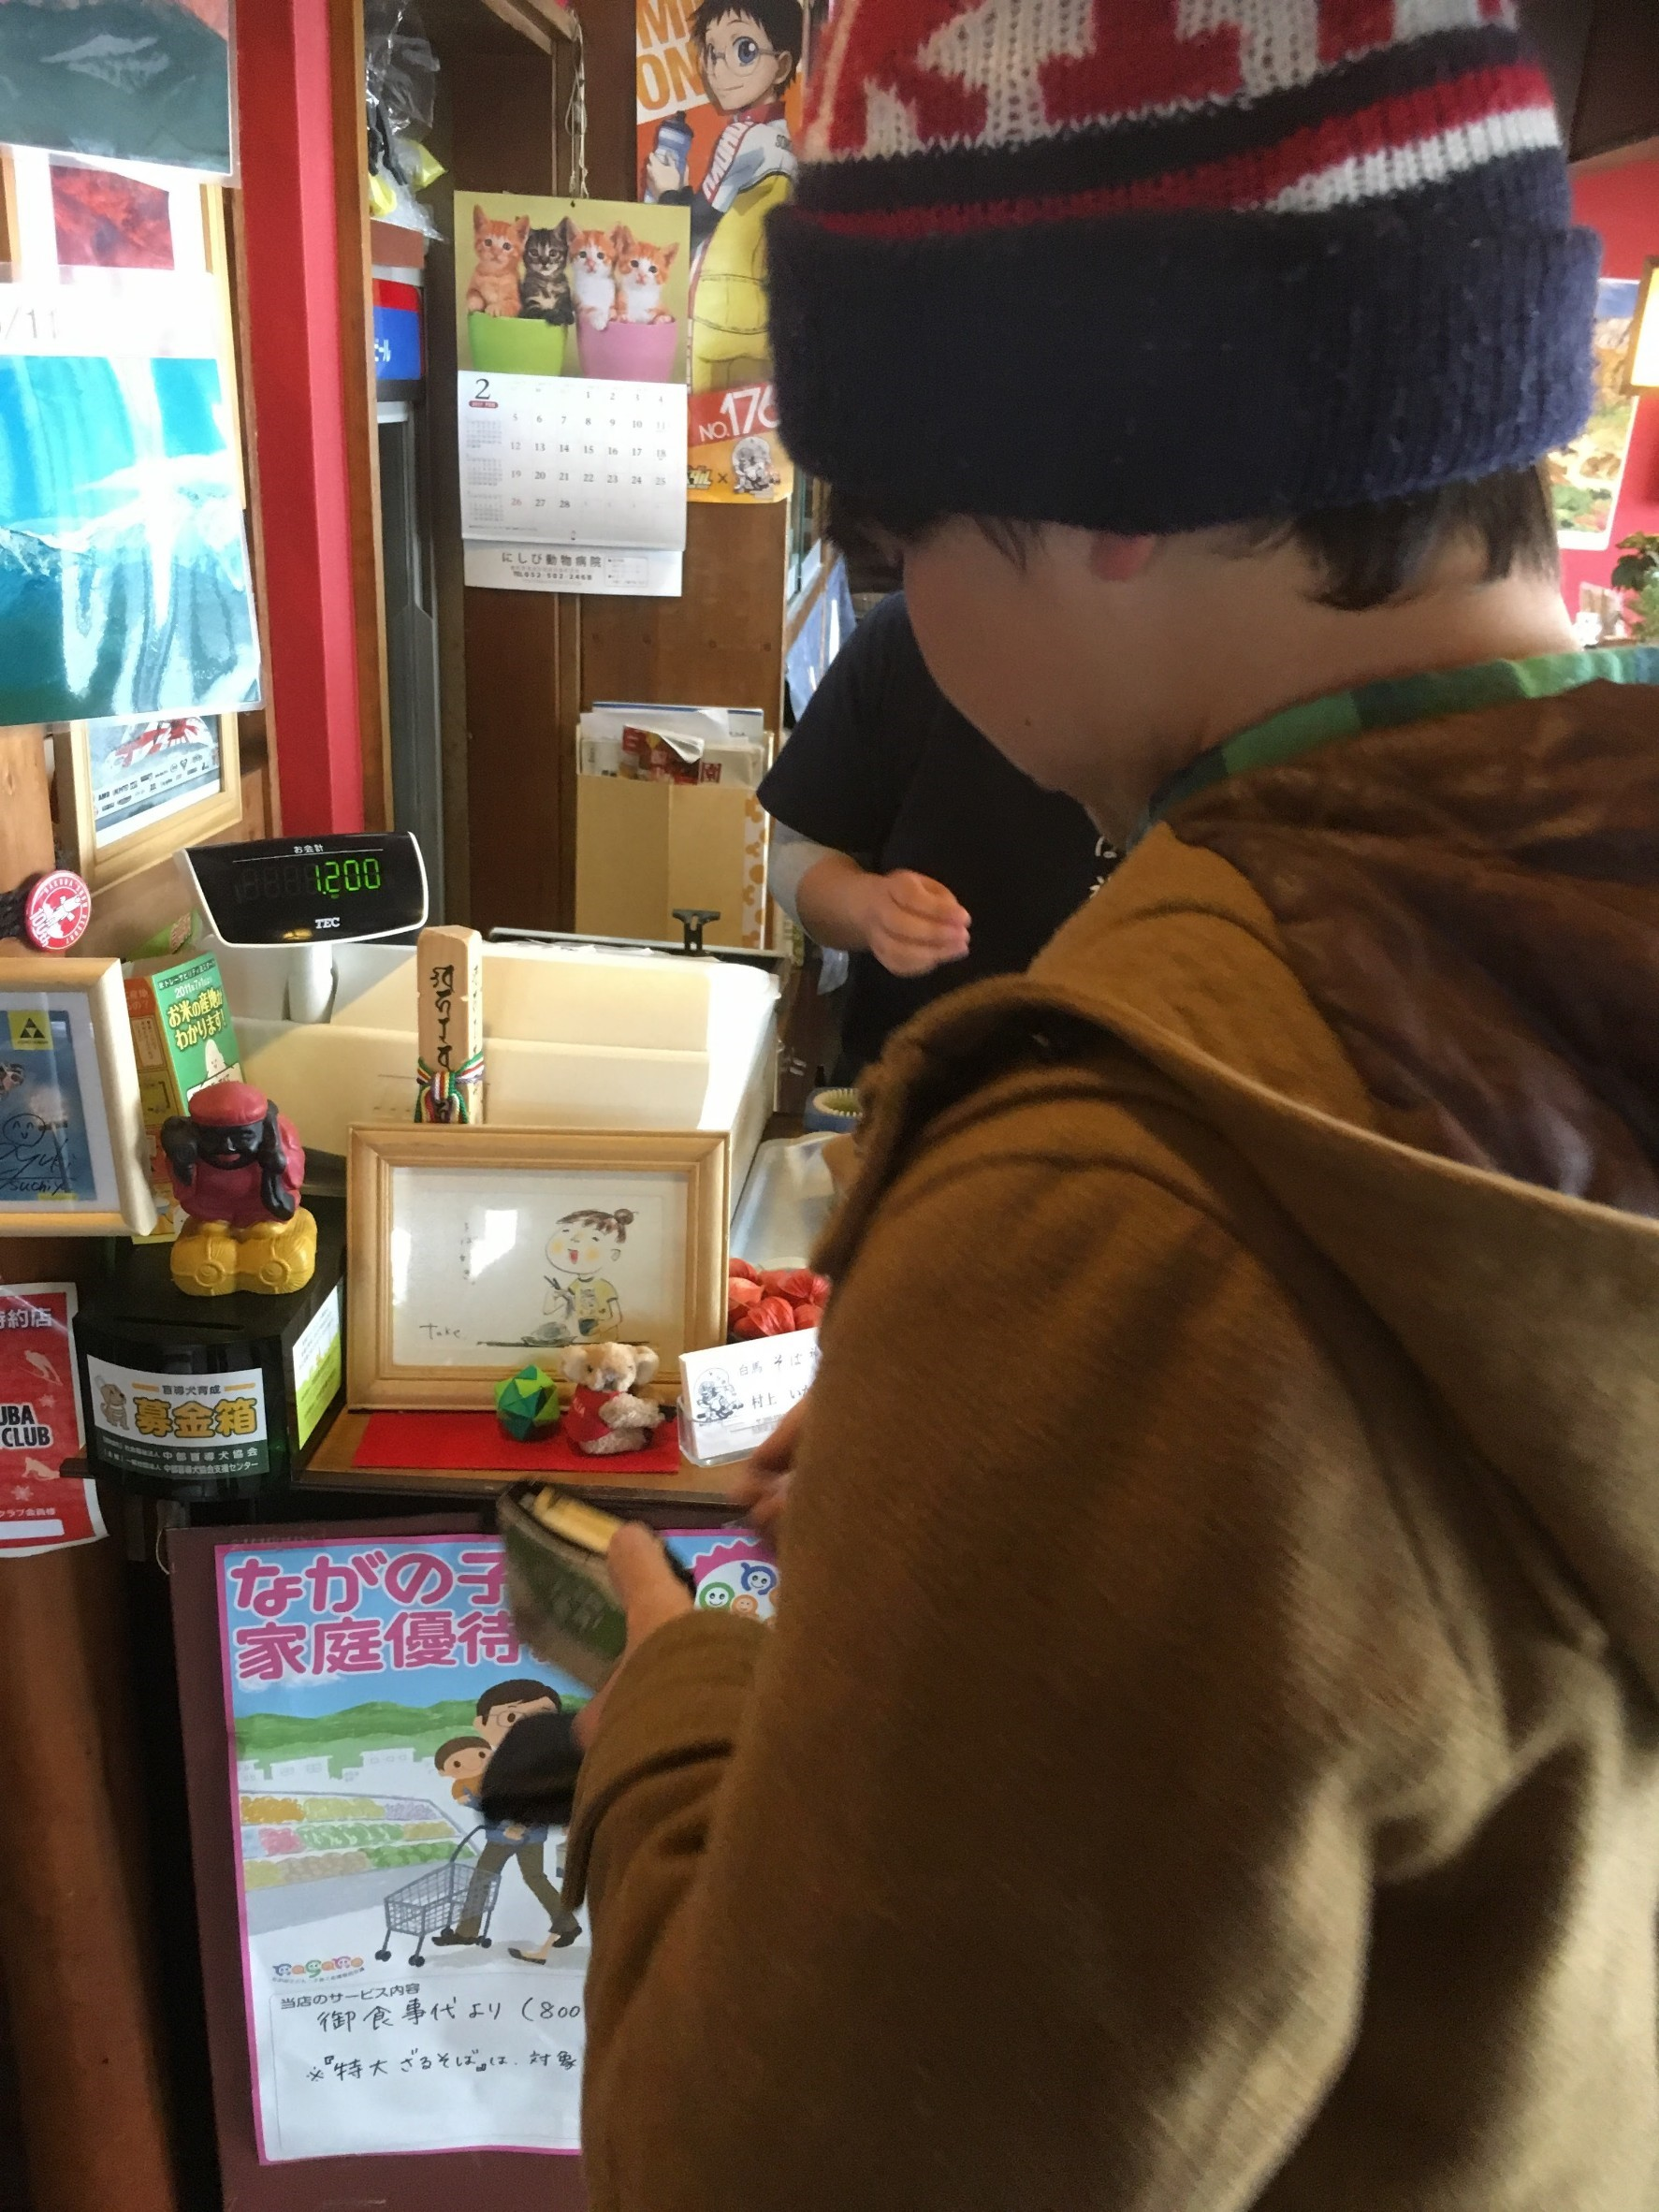
\includegraphics[width=0.4\textwidth]{./section/Shokuji/figures/SobaNido.jpg}

  \caption{開発した新手法を用いて、1200円で二度味わった。どこか誇らしげに財布を取り出し、支払いをする様子が見て取れる。うどん派の言い分として「蕎麦はお腹にたまらず食べた気がしない」との主張があるが、この新手法を用いれば、そのような主張は一蹴することができよう。}
\label{Fig:SobaNido}
\end{figure}
% ----------------------------------------



% ----------------------------------------
\begin{figure}[h]
\centering
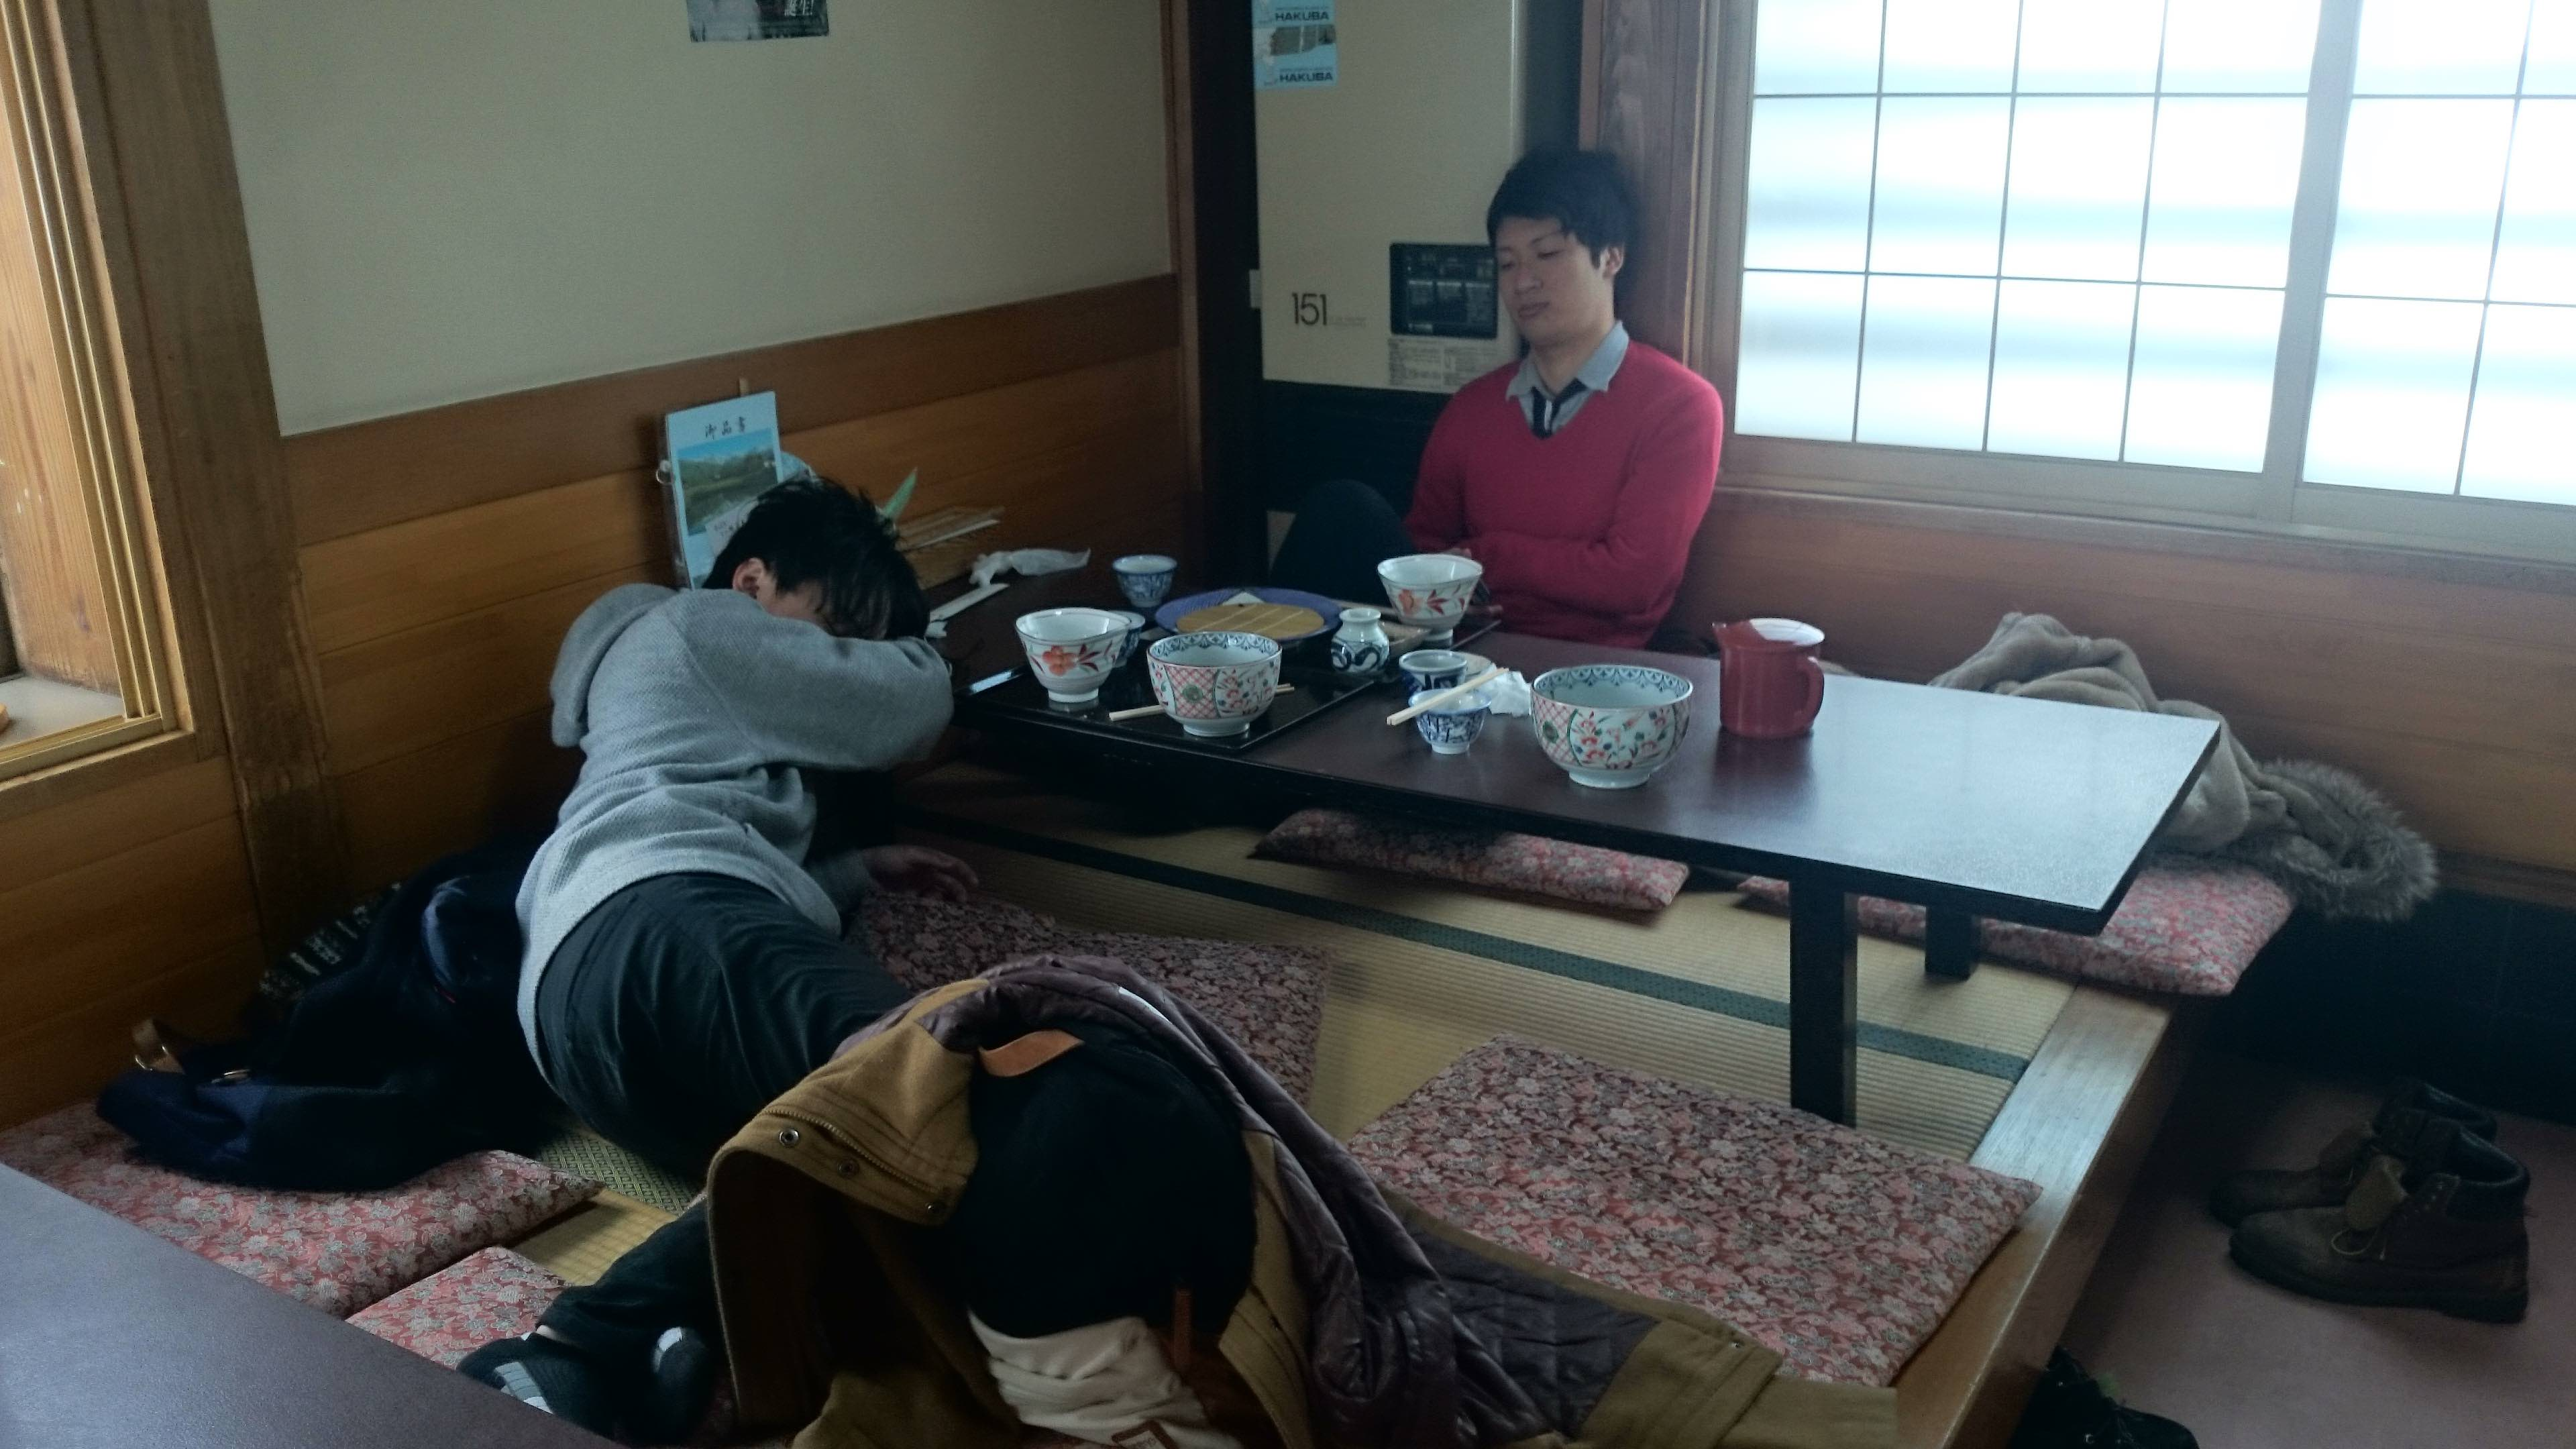
\includegraphics[width=0.6\textwidth]{./section/Shokuji/figures/Soba.jpg}
  \caption{副作用により、死人と化した。}
\label{Fig:Shigehisa}
\end{figure}
% ----------------------------------------

%%%%%%%%%%%%%%%%%%%%%%%%%%%%%%%
\section{自炊生活フロンティア}
%%%%%%%%%%%%%%%%%%%%%%%%%%%%%%%
最近は世知辛い世の中であり、いかにアベノミクスで日本経済が持ち直ったといえど、庶民の生活の改善には程遠いのが現状である。
そのため、世のサラリーマンを始め、学生も極力出費を抑えるため、自炊してお弁当を持ってくることが多いと言われている。
日本人といえば、白米であり、お弁当を作る際には白米と、何か簡単なおかずさえ作ってしまえば、一応お弁当の体裁は整えることができる。
しかし、おかずを作るのにも、数百円はかかっており、もちろん外食するより格段に安いため出費を抑えることができるが、自炊フロンティア(もしくは自炊生活末期症状)では、おかず作成に数百円を費やすことでさえ億劫に感じられているのが現状である。
そこで、自炊フロンティアでは、おかずとして駄菓子のわさびのり、蒲焼さん太郎、酢だこさん太郎をチョイスすることにより、一食にかかる費用を概算で約10分の1以下に大きく削減することが出来たのである。
% ----------------------------------------
\begin{figure}[h]
\centering
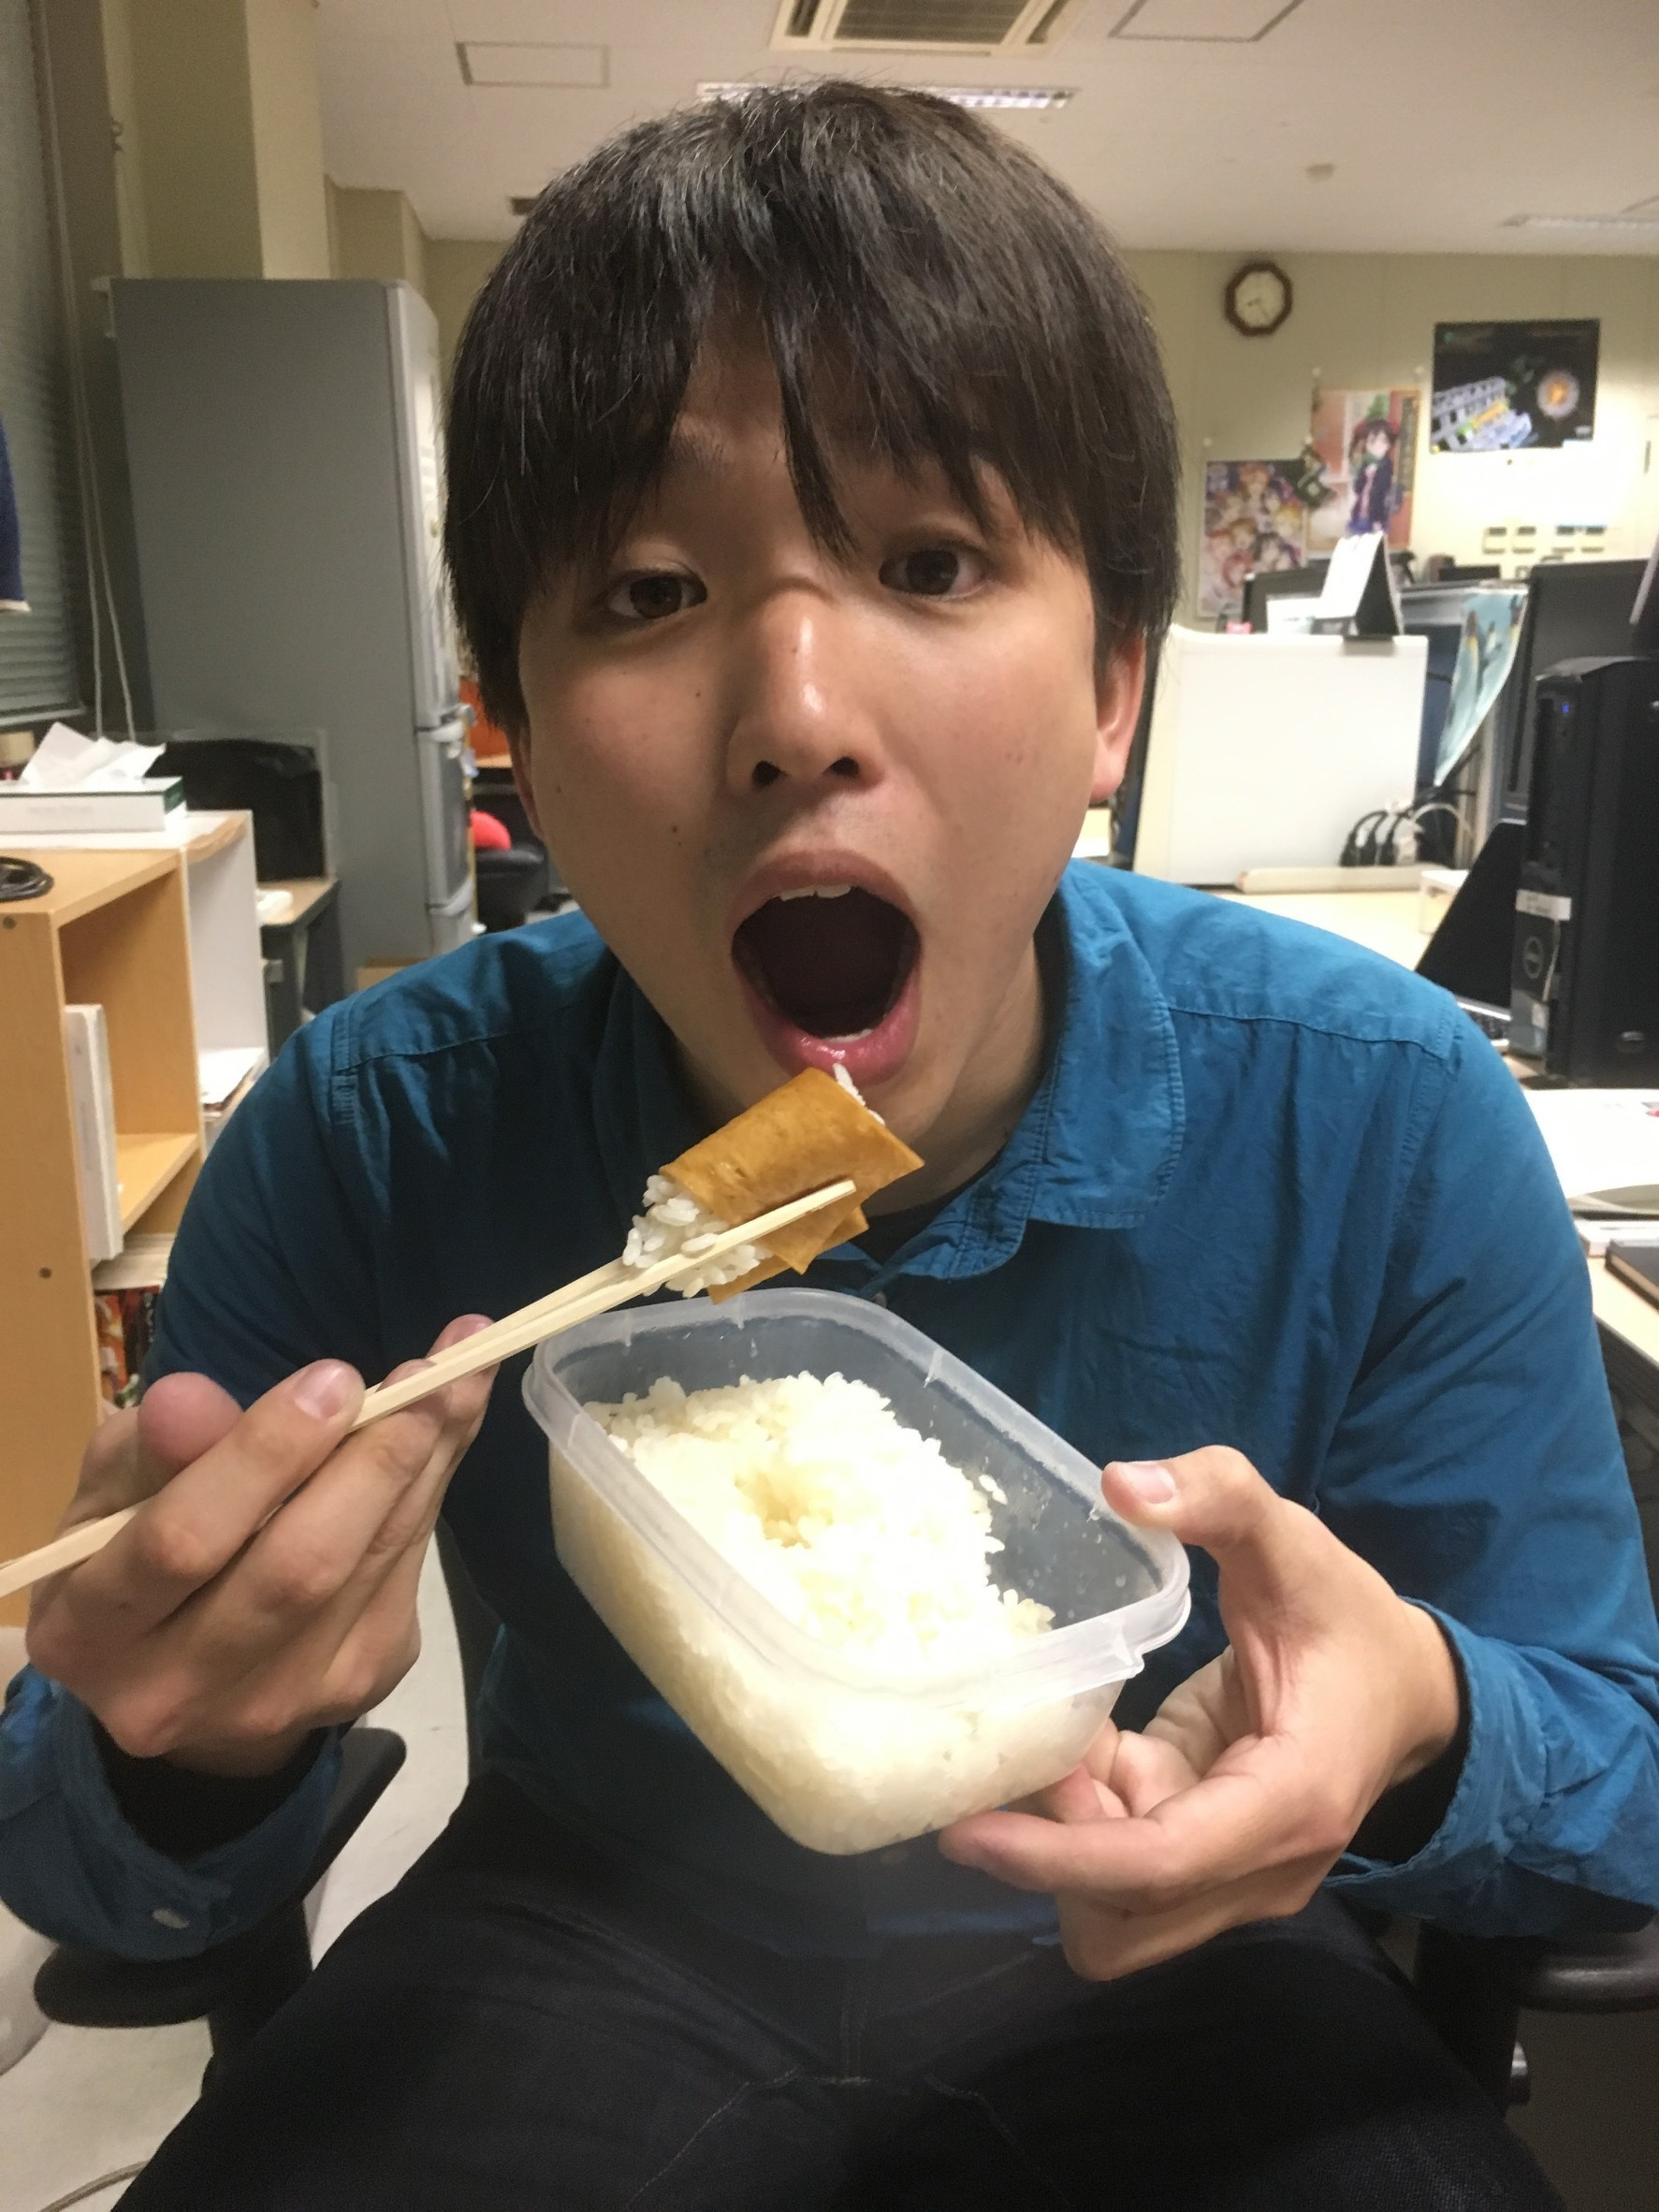
\includegraphics[width=0.4\textwidth]{./section/Shokuji/figures/JisuiMakki.jpg}
  \caption{流行りの弁当男子。持参した白米と、セブンイレブンで購入した駄菓子との最強コラボで晩ごはんを耐えしのぐ、涙ぐましい学生の姿である。小学生の頃は、蒲焼さん太郎ひとつ取っても、非常に心躍るものであったが、それから10数年たった今では、駄菓子とはこれほどまでに虚しいものであるのか、と改めて実感した。}
\label{Fig:Shigehisa}
\end{figure}
% ----------------------------------------


%%%%%%%%%%%%%%%%%%%%%%%%%%%%%%%
\section{アブラ足りてますか?}
%%%%%%%%%%%%%%%%%%%%%%%%%%%%%%%
「アブラ足りてますか足りてますか?」に対して「充分に足りている」と答えた場合、それは重症患者であろう。
一般人にとって、アブラとは食事の際にしか触れない概念であるが、重症患者の場合、食事の枠を飛び越え、日常的にアブラに接しているのである。
一年の計は元旦にあり、という有名なことわざを拝借するなら、重症患者にとって「一日の挨拶はアブラにあり」であろう。
すれ違う際、何かを叫ぶ際、熱いものに触ってしまった際、等で重症患者は「アブラ」を口にしてしまう。


% ----------------------------------------
\begin{figure}[h]
\centering
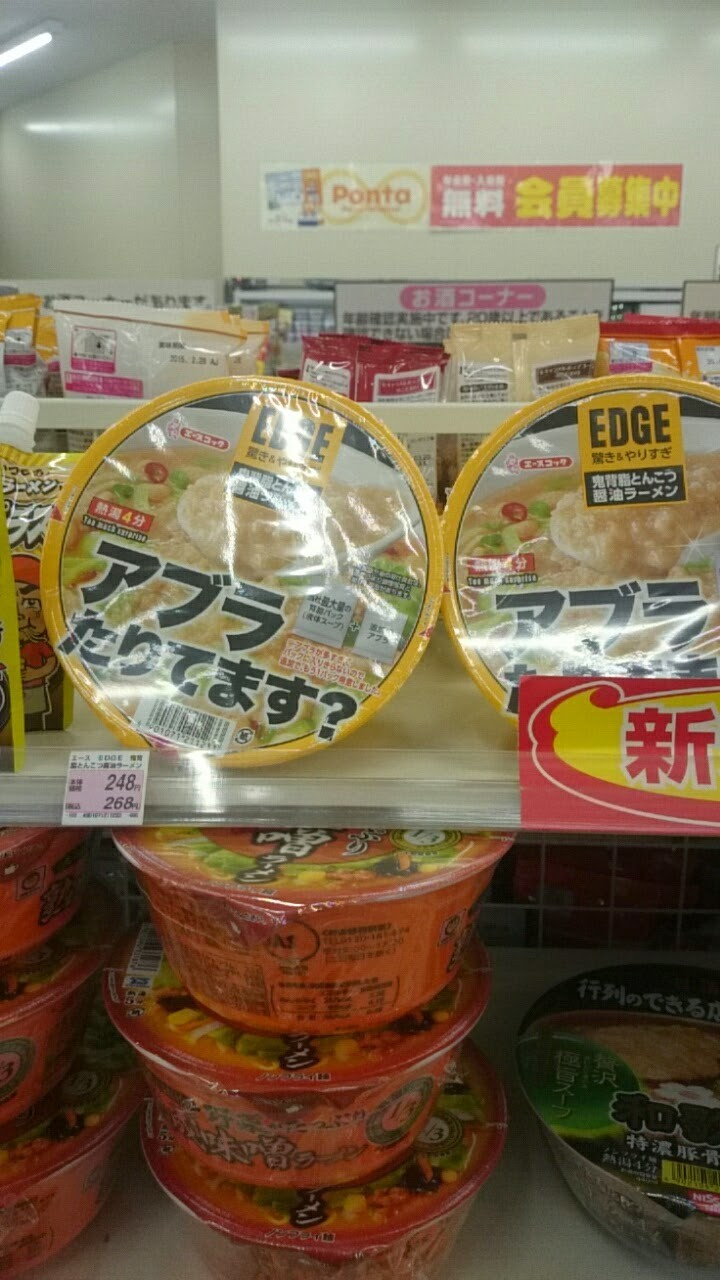
\includegraphics[width=0.4\textwidth]{./section/Shokuji/figures/AburaTaritemasuka.jpg}
  \caption{十二分にアブラは足りている。しかし、現代人にはアブラは不足していると言えよう。}
\label{Fig:Shigehisa}
\end{figure}
% ----------------------------------------

%%%%%%%%%%%%%%%%%%%%%%%%%%%%%%%
\section{リプトンタワー}
%%%%%%%%%%%%%%%%%%%%%%%%%%%%%%%
食事をより楽しくするものとして、西洋では食中酒という文化が広く知られている。
日本でも食事に合う酒、その中でも魚介類に会う酒、肉類に会う酒、などなど非常に幅広く食中酒が普及している。
その中で、食中を超え、いついかなるときでもリプトンと、いついかなる時でも烏龍茶を飲み続けた男たちがいることを、皆さんは御存知だろうか?
彼らは、食事以外でも暇を見つけてはリプトン・烏龍茶を飲み続けたのである。
ではなぜ彼らは、このような偉業を達成できたのであろうか?それは一つの小さな不満に端を発しているのである。

%==========================%
\subsection{引き出しという概念}
%==========================%
彼らが配属された研究室は、平たく言えば、席の当たり外れが非常に大きかった。
その不公平姓は席の位置に始まり、本来であれば一人一個分配される移動式引き出しがないデスクも存在したのである。
席の位置は、例えば図書館にこもったりすれば特に不満を感じないが、備品に関する不公平性は、その備品が分配されない限り解消されないのである。
確かに、近年は科研費の縮小や国家予算の再分配に伴い、備品にかける金額も限られてくるのが現状である。
特に配属されたての4回生への備品など、最もプライオリティの低いものであることは認めざるを得ない。
しかし、移動式引き出しの有無は、実行的なデスクの拡張、教科書置き場、として使うことができ、作業効率に関わってくるところである。
そこで、彼らは、なんとかしてこの移動式引き出しを自分たちで用意できないかと、その方法を模索していたのである。

%==========================%
\subsection{リサイクルという概念}
%==========================%
そんななか$1L$リプトンを飲んでいた男が、ひらめいたのである。
科学史において、ひらめきとは重要であり、エジソンも「ひらめきはナンチャラ」と言っていたくらいなので、非常に重要である。
かの有名なベンゼン環を発見したベンゼン氏は、睡眠している最中に蛇が自らのしっぽをかみ、輪になっている光景を見たことに閃き、それまででは考えられていなかった輪になっている化学構造を思いついたのである。
おそらく、これは推論であるが、リプトンからの閃きも寝ている最中に、はたと気づき「この空き容器を集めれば、簡単に引き出しが作れるのではないか?」と思いついたのであろう。
さらに、空き容器とは本来ゴミであり、リサイクルの観点からも非常に好感の持てる発想であり、人類の英知とも言えよう。
その動きに呼応するように、「私は烏龍茶で援助する」と名乗りをあげた人物がおり、彼ら二人をもってここに移動式リプトン・烏龍茶型引き出しの作成が始まったのである。

%==========================%
\subsection{積んでおくという概念}
%==========================%
しかし、引き出し建設には、非常に多くの空き容器が必要であることが、当時の試算でわかっており、
建設に必要な本数が集まるまで、5本一組の構造体にして積み上げる形で保存しておくこととなった。
一段、また一段と積み上がっていく度に達成感を感じ、次第に当初の目標であった引き出し作成よりも、天井まで届くタワーの建設へと目的がシフトしていった。
図\ref{Fig:LiptonTower_tochuu}に示すように、建設途中のリプトンタワーはある程度の高さまでいくと、不安定になるため、天井との間に突っ張り棒を敷いて耐震補強していたことが分かる。
また、その突っ張り棒には、その時に1年遅れくらいでハマっていた「あまちゃん」の主演女優の能年玲奈の写真が飾られている。

このタワーの色味からも分かるように、当初はリプトンから始まった建設であるが、一人の烏龍茶界の天才により、タワー構成の半分以上が烏龍茶となっていることが見て取れる。
この烏龍茶の成長率は、タワー建設計画終了まで持続されることとなる。
ここまでに、リプトンと烏龍茶の構成率の違いが現れた原因として、値段が1.5倍違うことが挙げられよう。
リプトンは150円ほどであり、烏龍茶の方が安いのである。
また、健康面からも一日に何本もリプトンを飲むことはあまり好ましくなく、その点、烏龍茶は何本飲んでもなんとなく大丈夫であるとの観点から、構成率に大きな差を生んでいる。
さらにその構成率の違いに拍車をかける決定打は、リプトンのリニューアルである。
従来のパッケージを新しいものに置き換えたところまではよかったのであるが、なんと内容量もリニューアルされ、従来の1リットルから950ミリリットルへと削減されたのである。
このことから、リプトンを買うコスパの悪さが構成率の違いを生み出したと言っても過言ではない。


% ----------------------------------------
\begin{figure}[h]
\centering
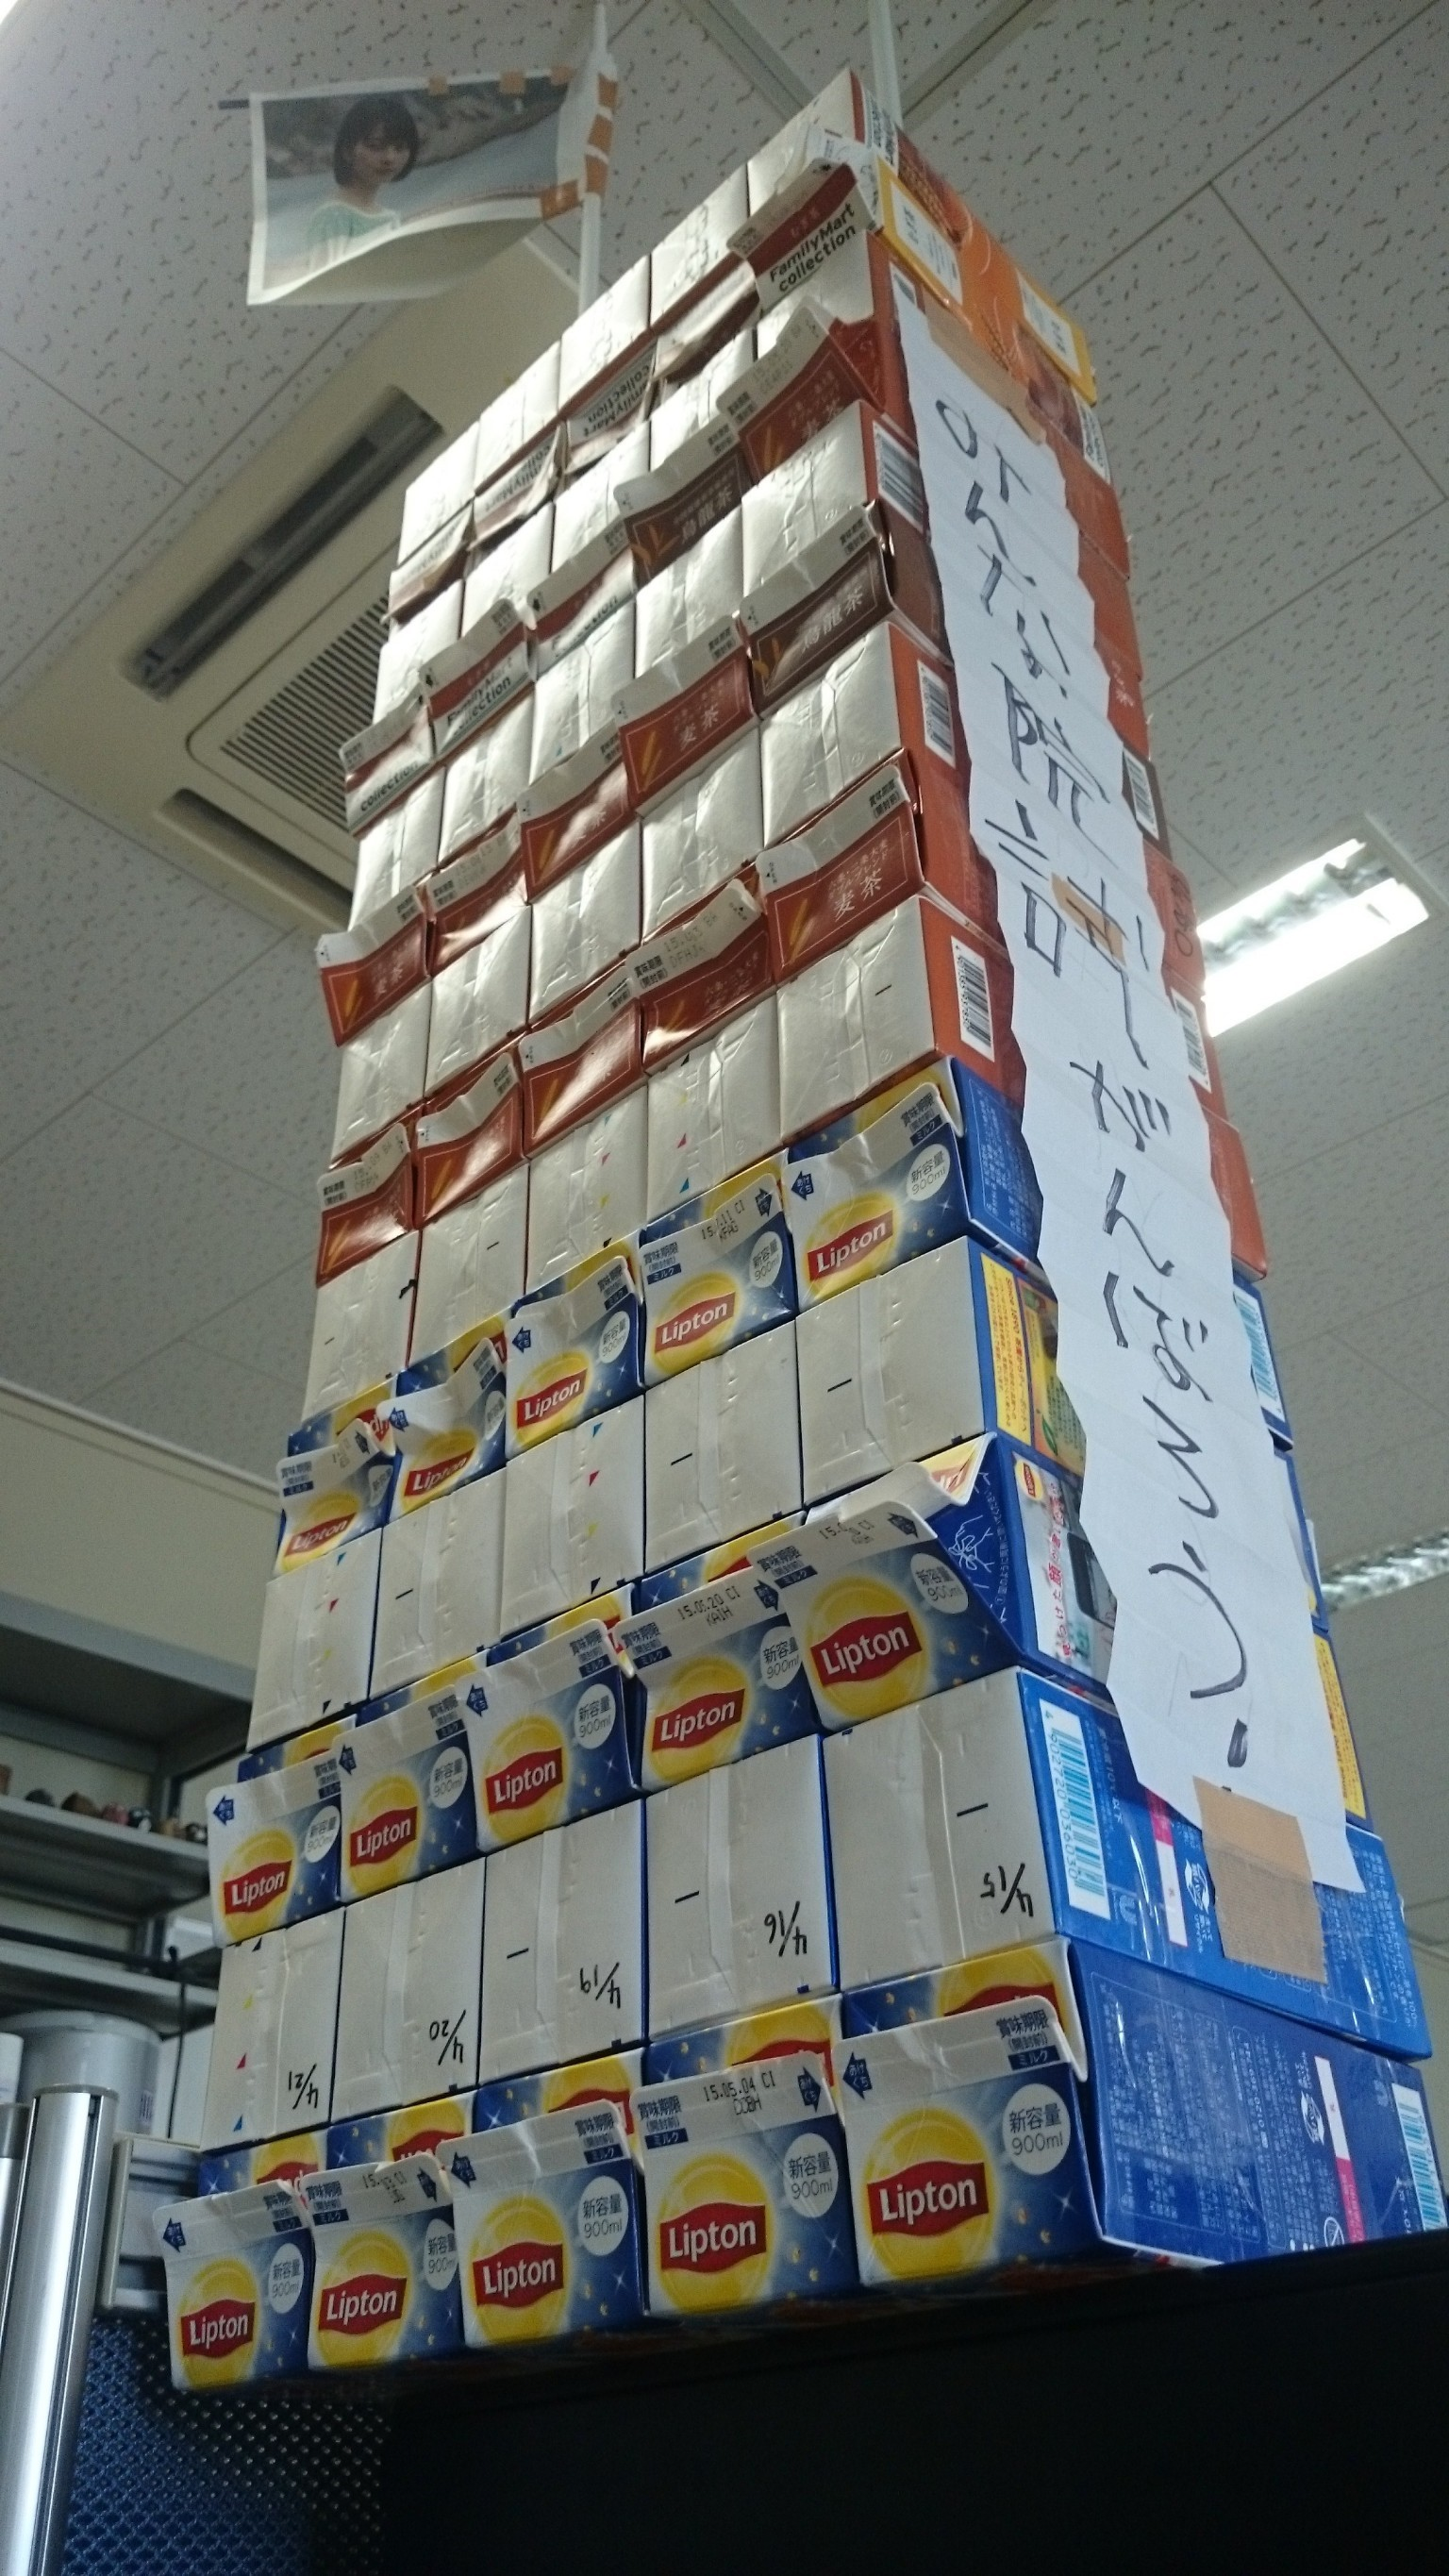
\includegraphics[width=0.4\textwidth]{./section/Shokuji/figures/LiptonTower_tochuu.jpg}
  \caption{引き出し作成のための建材を保管している様子。「みんな院試がんばろう!」と書かれた横断幕が貼られていることからも、この建材置き場は、学生の交流の場として活かされていたことも分かる。}
\label{Fig:LiptonTower_tochuu}
\end{figure}
% ----------------------------------------

%==========================%
\subsection{風邪なのに飲み続けるという概念}
%==========================%
リプトンマンをさしおいて、烏龍茶男は雨の日も風の日も、風邪の日も烏龍茶を飲み続けた。
どれだけ咳き込んでいようとも、烏龍茶を飲んで喉を冷やし続け、風邪を悪化させ続けた。
このように涙ぐましい努力も、構成に語り継いでいくべきであろう。

%==========================%
\subsection{高さ調整のために電磁力学の教科書を使うという概念}
%==========================%
ようやく努力の成果が結実するときがきた。
タワー完成である。
しかし、デスクトップPCと天井との間には数cmの隙間が出来てしまうことがわかったのだ。
そこで機転を利かせ、電磁力学の教科書を挟んでおくことにした。
後に藏重教授から「そんなことしてるから電磁気の点数がアハアハアハ」となじられるのである。

% ----------------------------------------
\begin{figure}[h]
\centering
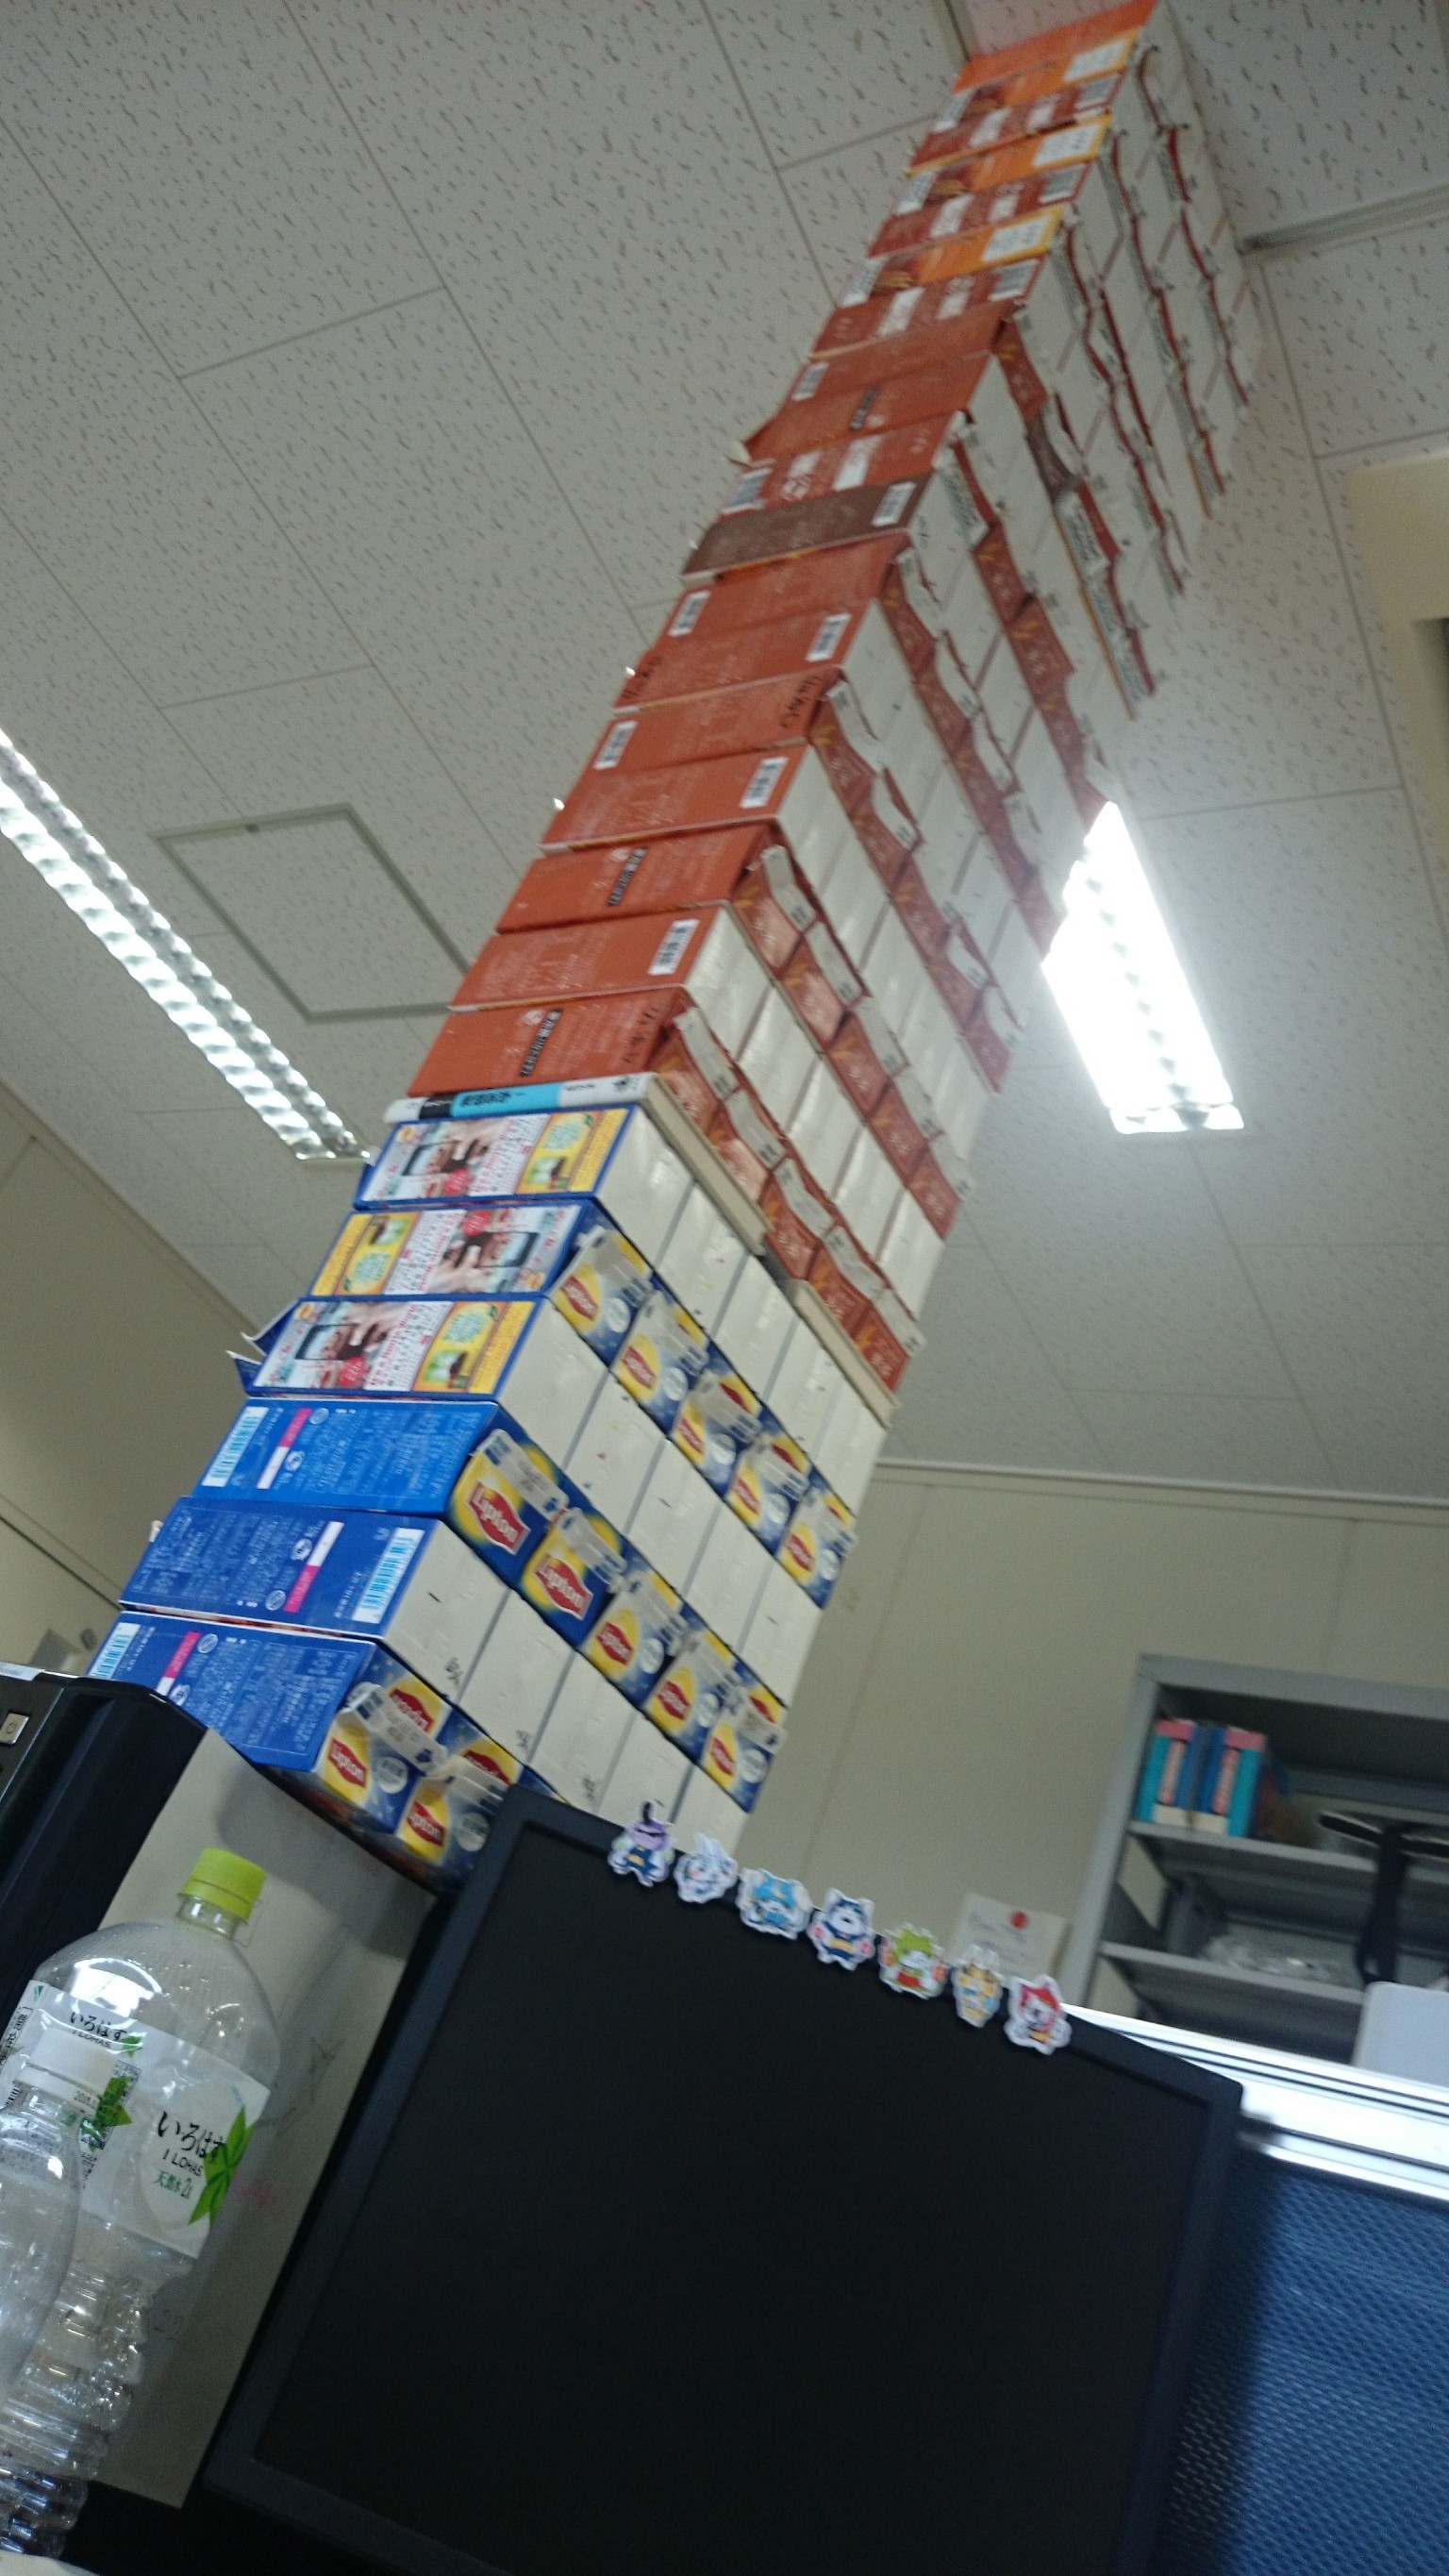
\includegraphics[width=0.4\textwidth]{./section/Shokuji/figures/LiptonTower_final.jpg}
  \caption{見事なタワーである。もはや色合いとしては、烏龍茶タワーと呼ぶべきかもしれない。建設後半タケダ氏は、烏龍茶の追い上げに度肝を抜かし、お茶飲みとしての才能に限界を感じ一線から退いたのである。ちなみに、このタワーの建設費用は概算で13500円である。}
\label{Fig:LiptonTower_final}
\end{figure}
% ----------------------------------------



%==========================%
\subsection{実は邪魔だったという概念}
%==========================%
このリプトンタワー、建設者からの視点では、特に問題なく積み上がっていたのであるが、それとは対照的に近隣住民の一声で計画が頓挫、建設企業の廃業にまで追い込まれたのである。\par
「この柱のせいで時計が見えへんから、捨ててこい」\par
なるほど、と感じた反面、別にええやろ、と感じたのは言うまでもない。


%%%%%%%%%%%%%%%%%%%%%%%%%%%%%%%
\section{日本人の精神}
%%%%%%%%%%%%%%%%%%%%%%%%%%%%%%%

% ----------------------------------------
\begin{figure}[h]
\centering
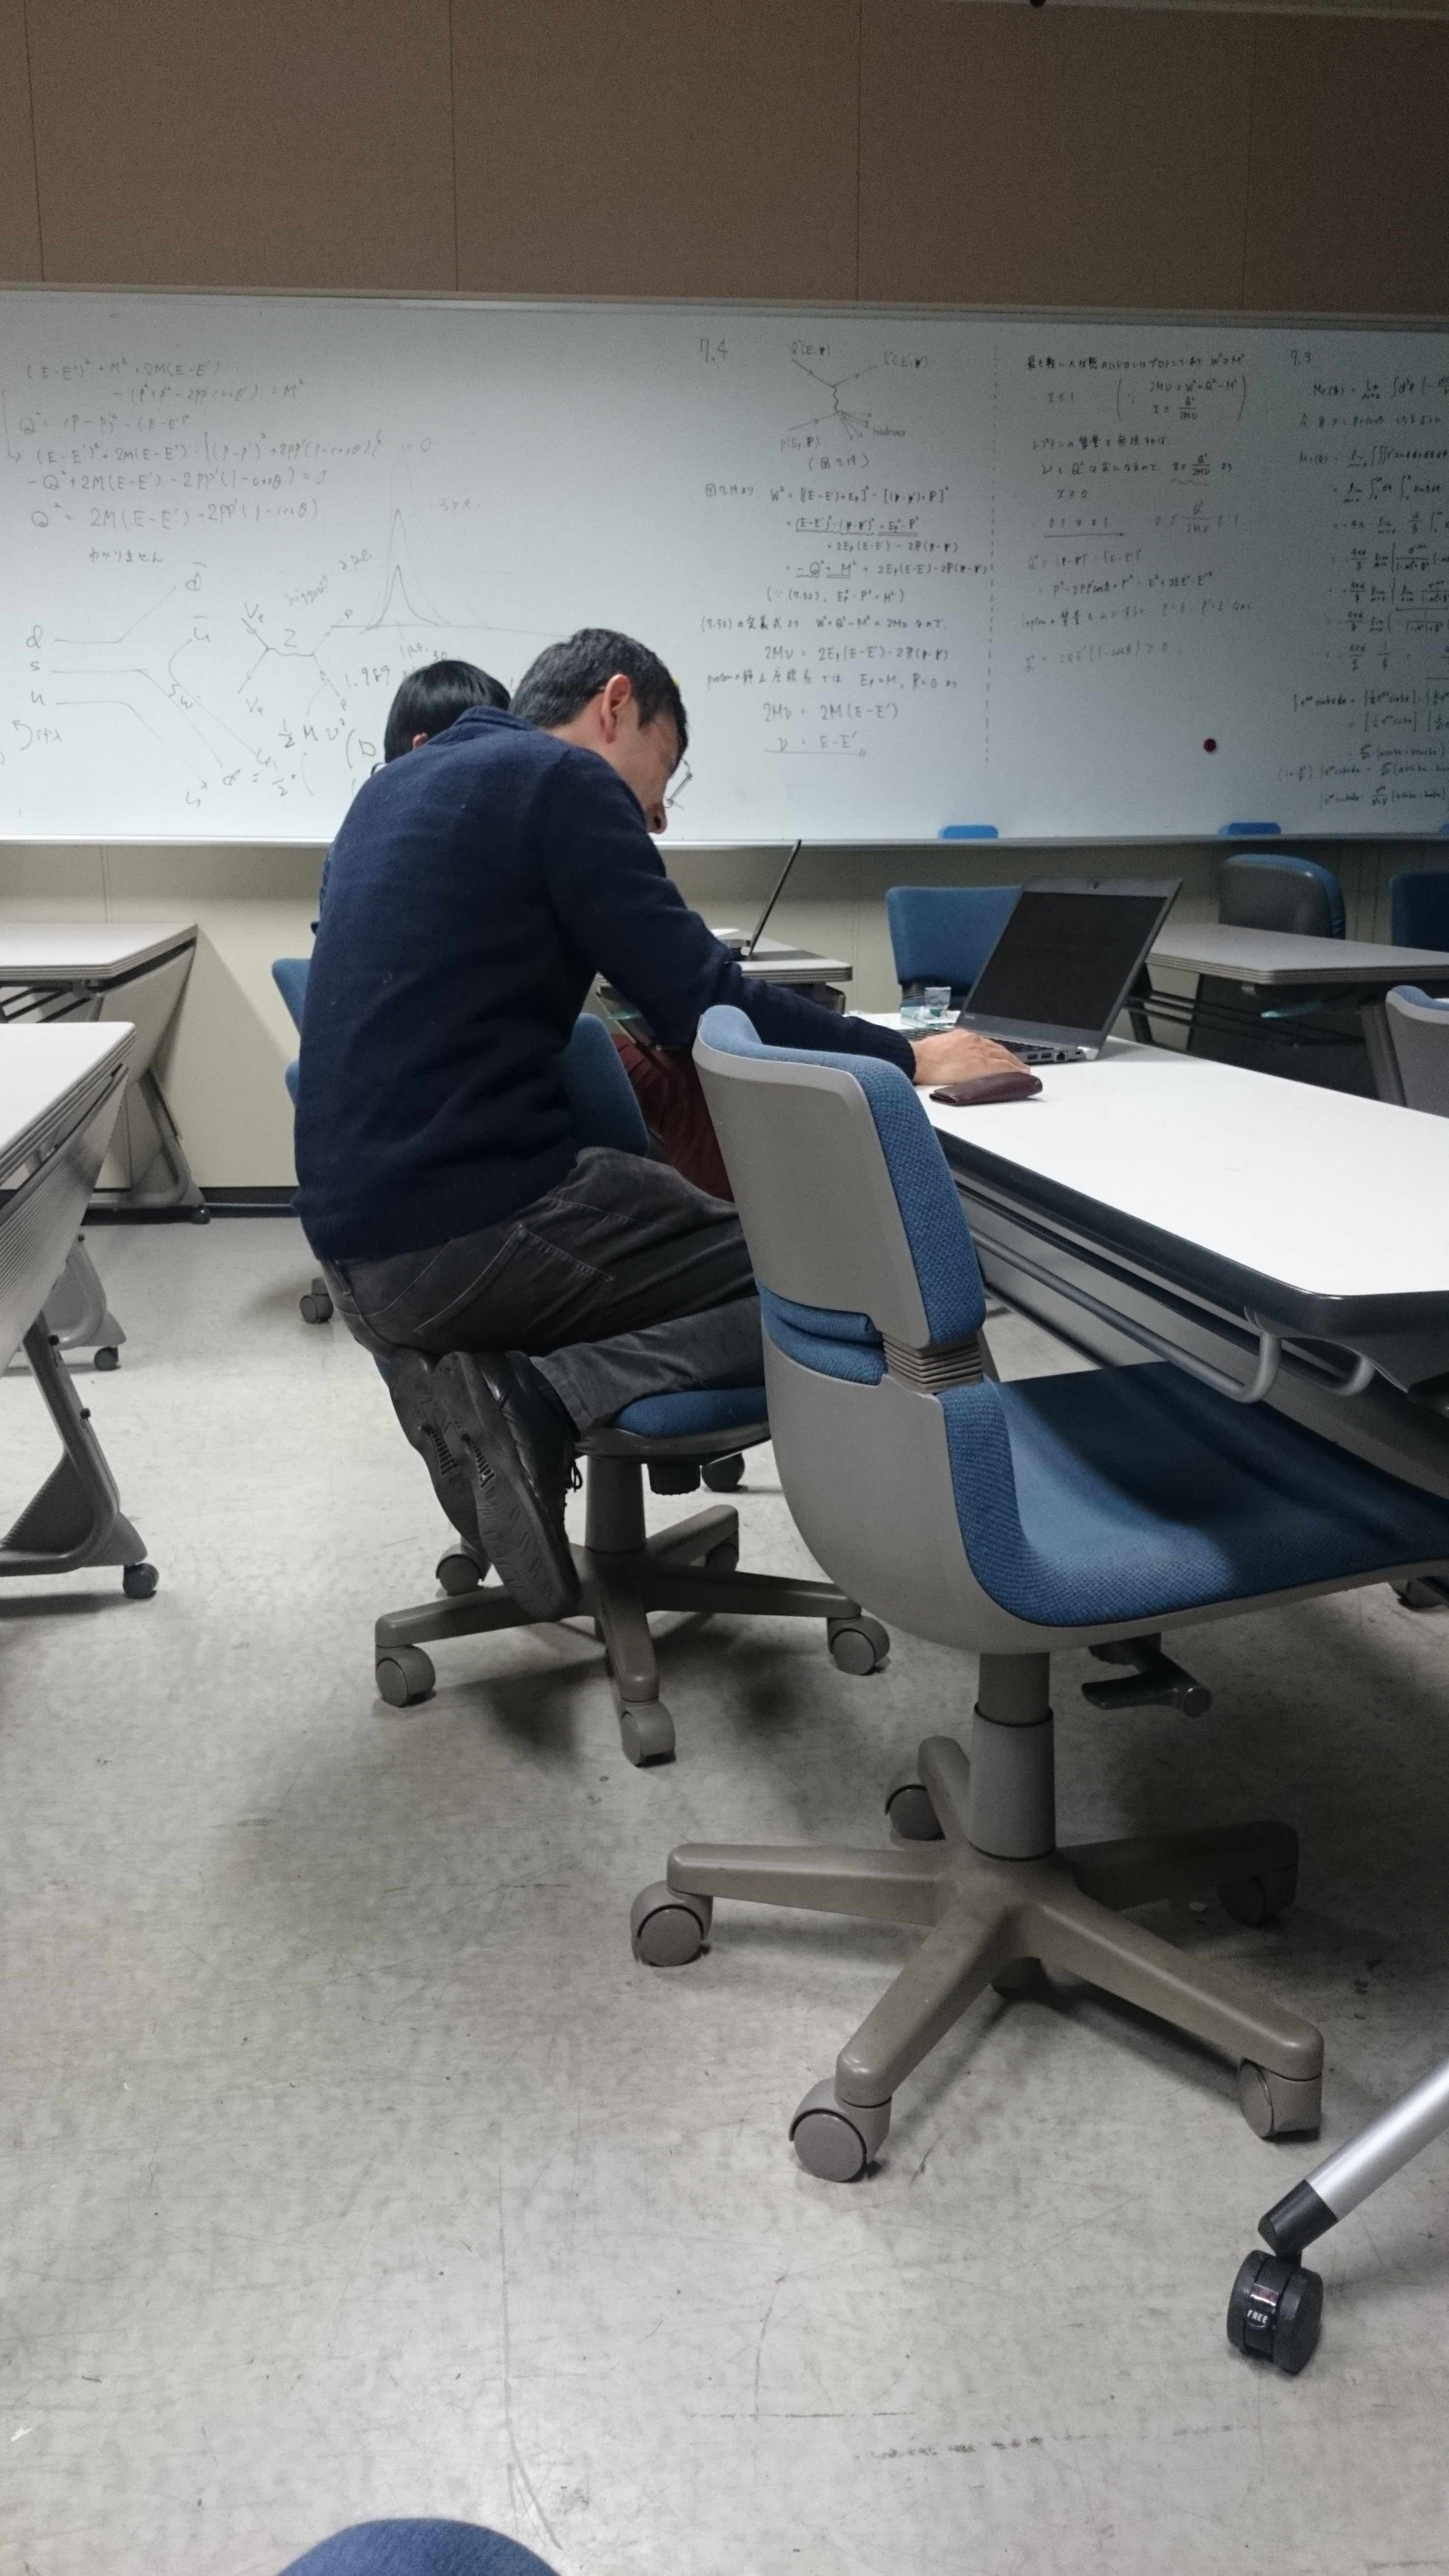
\includegraphics[width=0.4\textwidth]{./section/Shokuji/figures/Seiza.jpg}
  \caption{いかなるときも日本人の心を忘れず、椅子に座りつつ正座を行う}
\label{Fig:Seiza}
\end{figure}
% ----------------------------------------



%%%%%%%%%%%%%%%%%%%%%%%%%%%%%%%
\section{おばコーヒー}
%%%%%%%%%%%%%%%%%%%%%%%%%%%%%%%
世の中にはその人の名を冠した地名や建物などが多く見受けられる。
しかし、コーヒーにその名を残した偉人が未だかつて存在しただろうか?
現代に伝わる七不思議の一つ、それが「おばコーヒー」である。
このおばコーヒーというのは、生協オリジナルの上質なコーヒー牛乳であり、200mLしか入っていないのに100円するという、穿った見方をすればボッタクリのような商品であるが、消費者を魅了してやまないのは、その独特の飲み方のスタイルにある。
普通に一般の方が飲むと、吸い終わった後に容器に空気が入る音で「ジュボッ」という音がする。
この飲み方では、そう、授業中には迷惑になって飲めないのである。
しかし、この飲み方に一石を投じた人間がおり、それが「おば」である。
このおば氏は、吸い終わった後、容器の中に空気が戻ることが原因で音がなるので、最初から飲む時に容器を押さえつけてなるべく空気の出戻りを少なくすれば消音できると提案した。
画期的な発見であることにその当時の学者は誰一人気づかなかったが、これが後に世界的に受け入れられ、開発したおば氏の名を冠し、「おばコーヒー」と一部の学者から呼ばれるようになったのである。

% ----------------------------------------
\begin{figure}[h]
\centering

\includegraphics[width=0.4\textwidth]{./section/Shokuji/figures/ObaCoffee.jpg}
  \caption{生協で売上トップをひた走る人気商品であればうれしいが、、、。見て分かるように、牛乳よりも多く展開されている商品である。ちなみにこの牛乳に関して、オガワ氏が飲み会の前に度々飲み「牛乳で胃袋に膜を張ってアルコール吸収率をうんぬんかんぬん」と言っていたが、その効果のほどは本人以外分からない。個人的には、牛乳飲んでも、ウコン飲んでも、死ぬときは死ぬ。}
\label{Fig:Seiza}
\end{figure}
% ----------------------------------------

%%%%%%%%%%%%%%%%%%%%%%%%%%%%%%%
\section{夕食の範疇を超越する}
%%%%%%%%%%%%%%%%%%%%%%%%%%%%%%%
原動機付自転車で神戸の街を颯爽と駆け巡る若者にとって、徒歩で数十分かかる場所へもラクラクとアクセスできるので、非常に行動範囲が広がる。
しかし、良い事ばかりではない。「お腹すいた」と思ったらすぐにどこかへ行けてしまう怖さも秘めているのである。
原動機付自転車に乗れば日頃の運動量が減るばかりではなく、ガソリンを使い脂肪を蓄えるため、様々な場所へ移動することになるのだ。


%==========================%
\subsection{すき家}
%==========================%
夜食とは、夕食を食べた後に小腹がすいてしまい、スナック菓子などに手が伸びてしまうことを言う。
では、夕食を食べずバイトが22時過ぎに終わり、お腹が空いてしまった場合はどうすればいいのだろうか?
その答えは近所のすき家に駆け込む、である。
何ご飯なのだろうか?と聞かれても、晩御飯の概念を超越しており、ただただ健康を害するだけである。
しかし彼らは20代も前半であり、まだまだ新陳代謝の衰えは感じていなかったのであろう。
「若い頃にむちゃするんじゃなかった」と思ってももう遅い、とキートン山田に突っ込まれそうである。

\begin{figure}[htbp]
% \begin{minipage}{0.5\hsize}
\centering
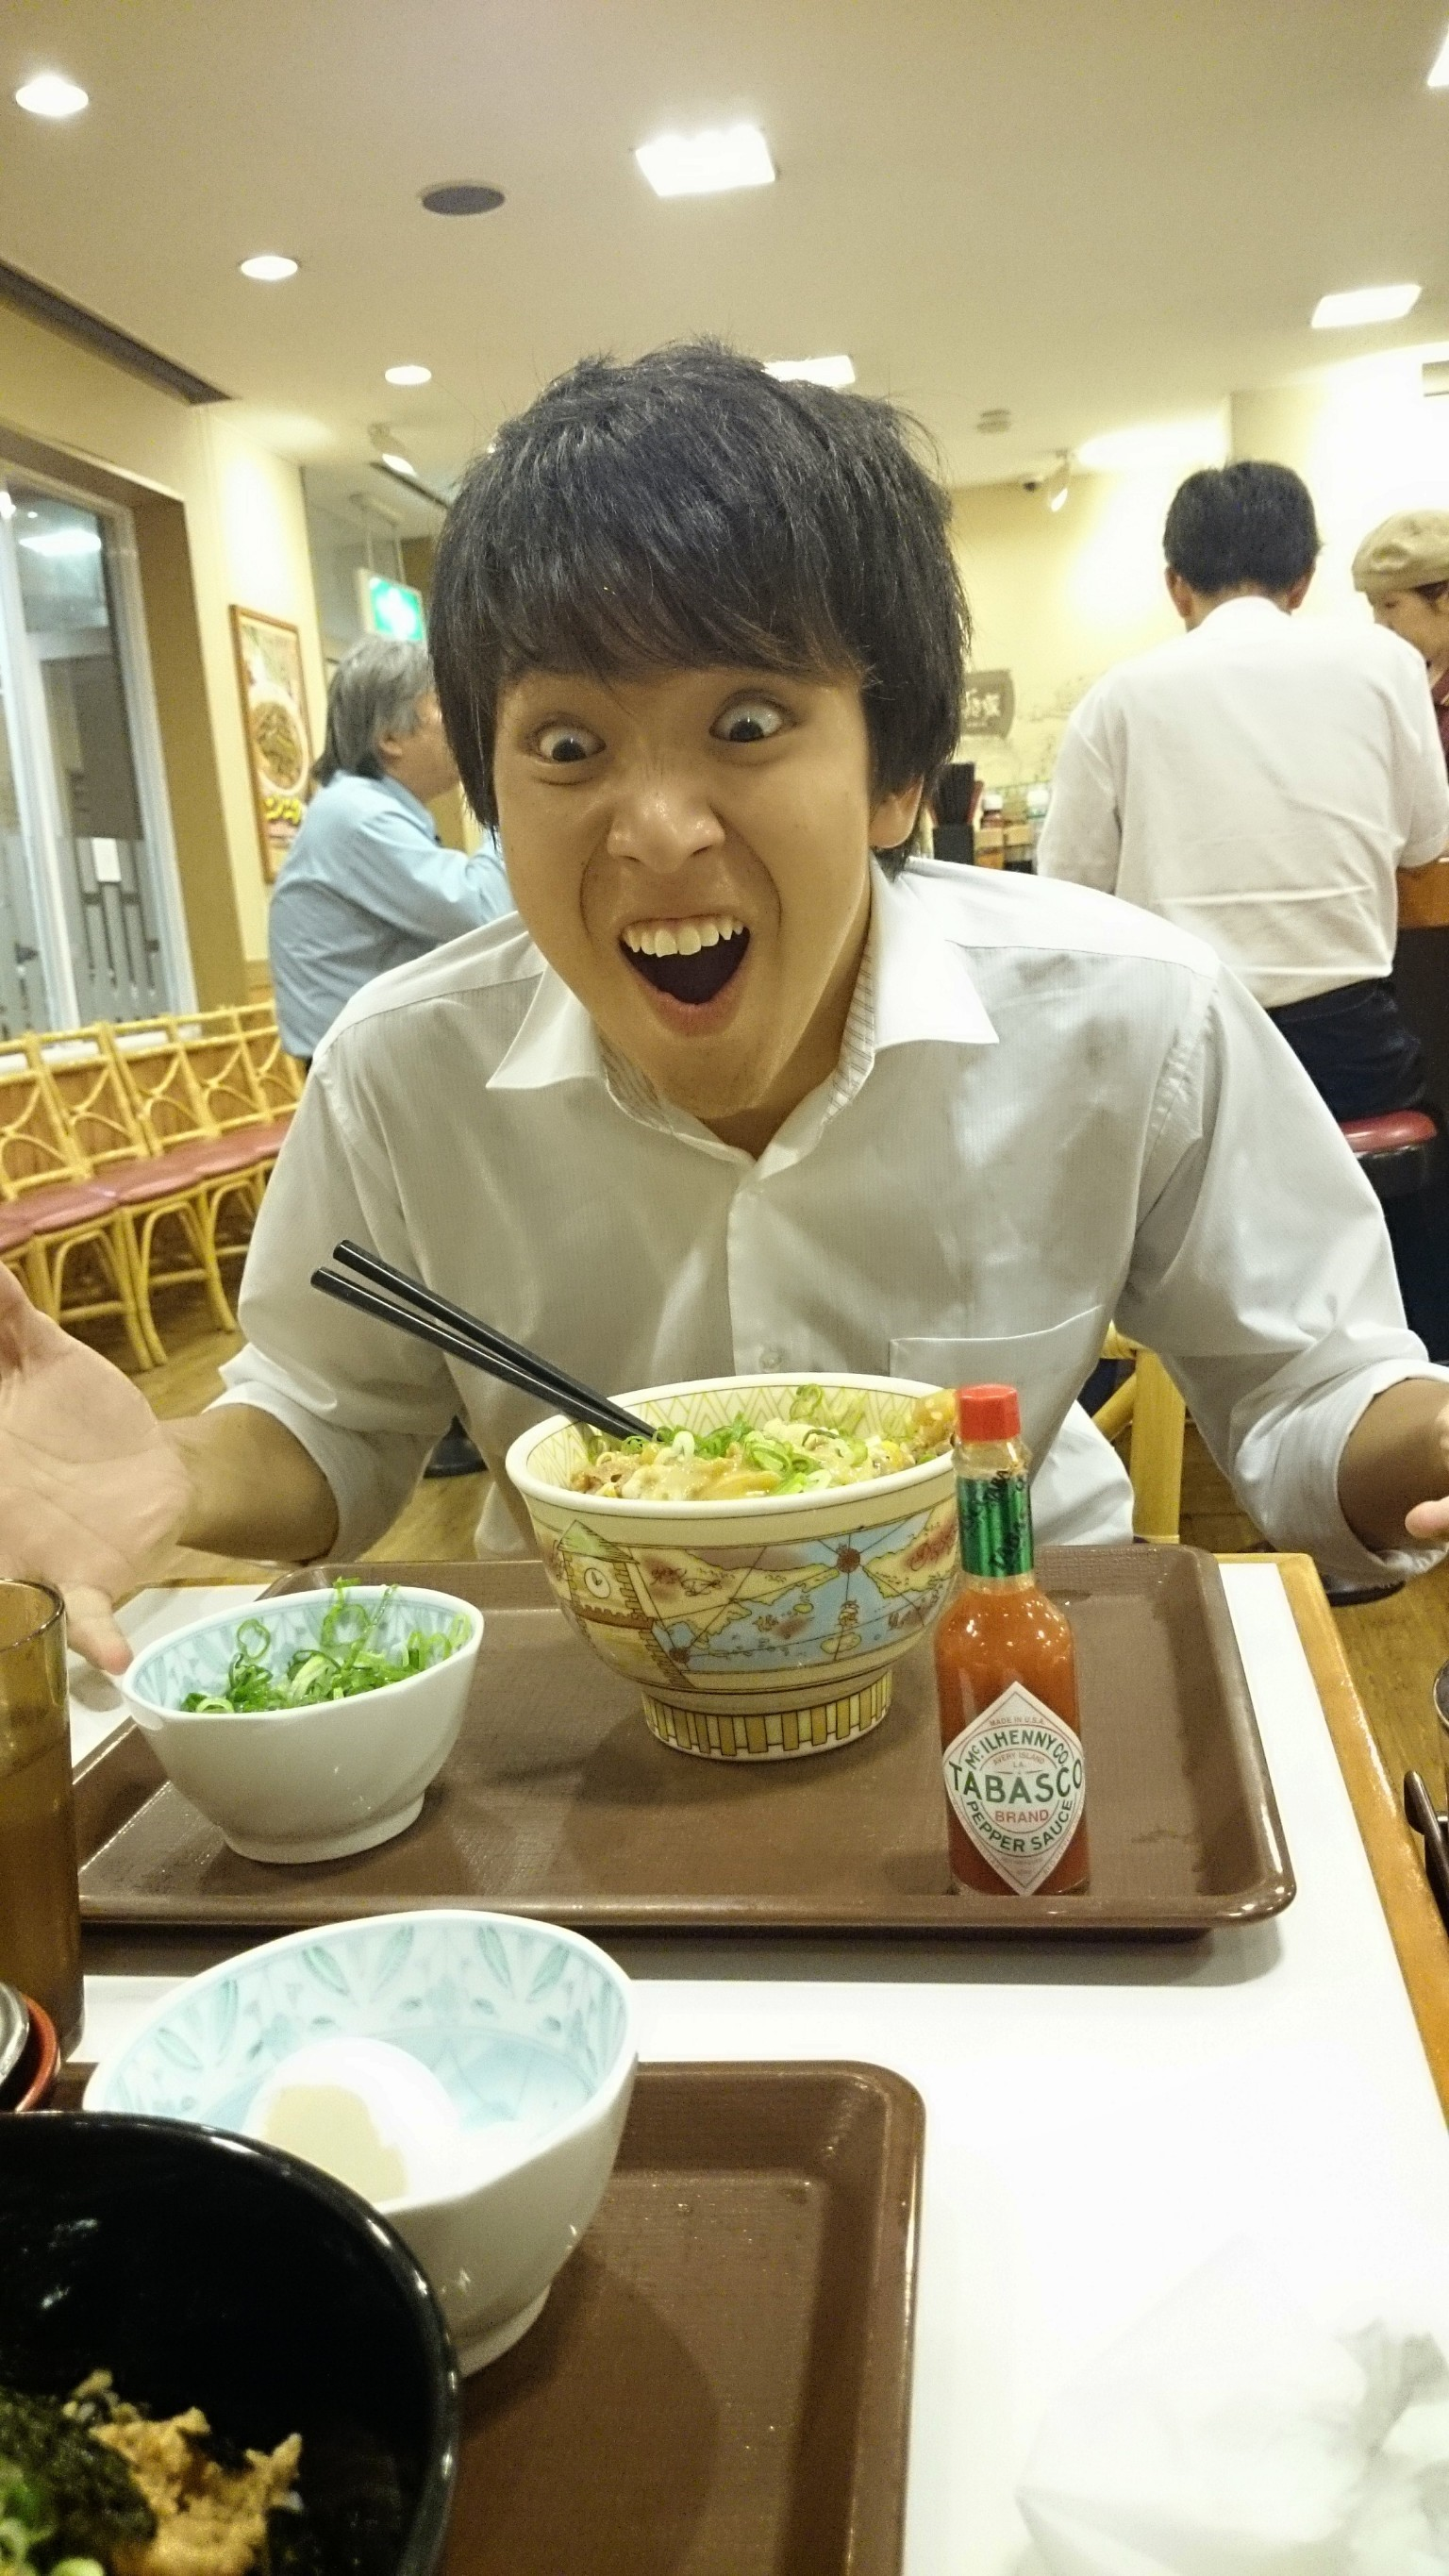
\includegraphics[width=0.3\textwidth]{./section/Shokuji/figures/LifeSukiya.jpg}
%  \end{center}
 \caption{とりあえず辛いもの食っとけの精神でタバスコを用意し、またネギ大盛り別皿はテッパンである。これをもりもり食べた後は、原動機付自転車を法定時速で運転し、家に帰って寝るだけである。}
  \label{fig:one}
\end{figure}
% \end{minipage}
% \begin{minipage}{0.5\hsize}
%  \begin{center}
\begin{figure}[htbp]
\centering
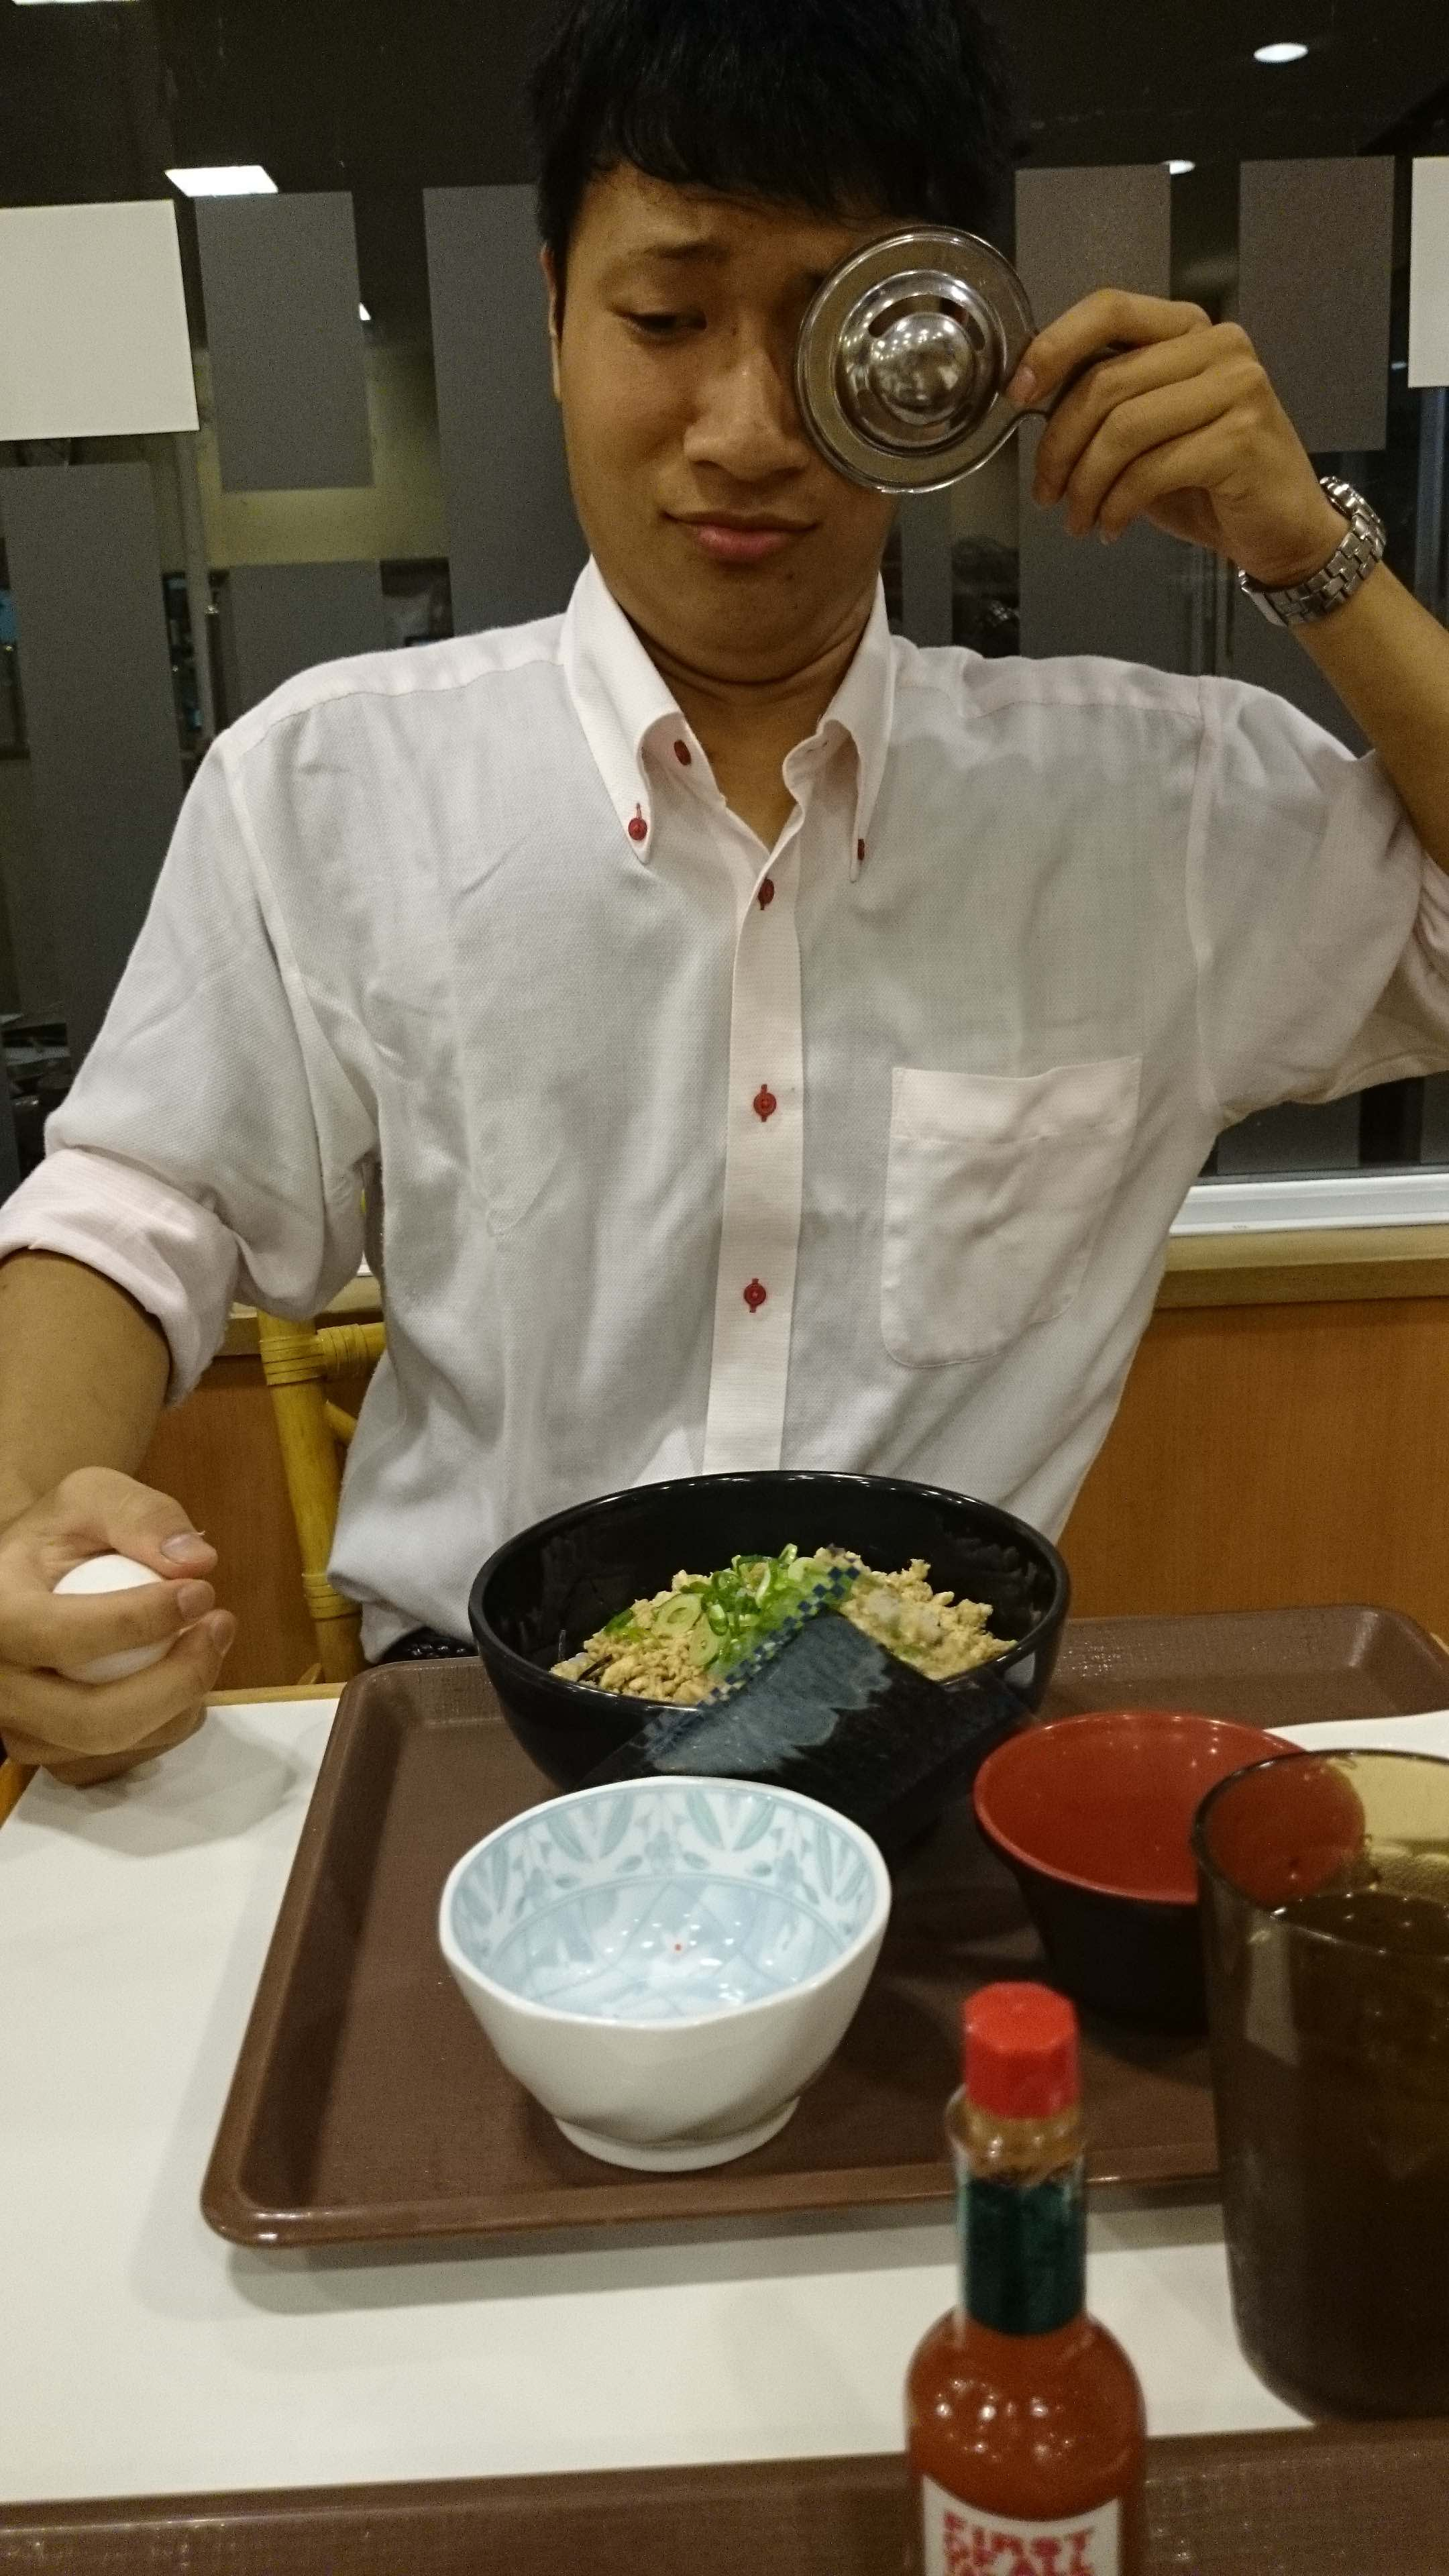
\includegraphics[width=0.3\textwidth]{./section/Shokuji/figures/LifeSukiya_2.jpg}
 \caption{この男はこの夜食を食った後、原動機付自転車を時速60km/hでぶっ飛ばし門限までに寮に帰らなければならないのである。さもなければ反省文を書かなければならない。法定時速を守るか、寮の規則を守るか。この男はあまりにも寮に忠実な(ちゃんと掃除会にも参加するし、なんか色々やるし)模範的な寮生なのであった。}
  \label{Fig:Ogawa}
\end{figure}

さらに、食べすぎたのか何なのか分からないが、別人とも言えるオガワの写真(図\ref{Fig:OgawaBetsujin})も現存している。
タケダ側のお盆を見ると、健康を気にしてサラダを頼んでいるが、焼け石に水、無駄な抵抗である。
それに引き換え、オガワは宙を見つめ、すべてを悟ったかのように己の運命を受け入れている。

% ----------------------------------------
\begin{figure}[h]
\centering
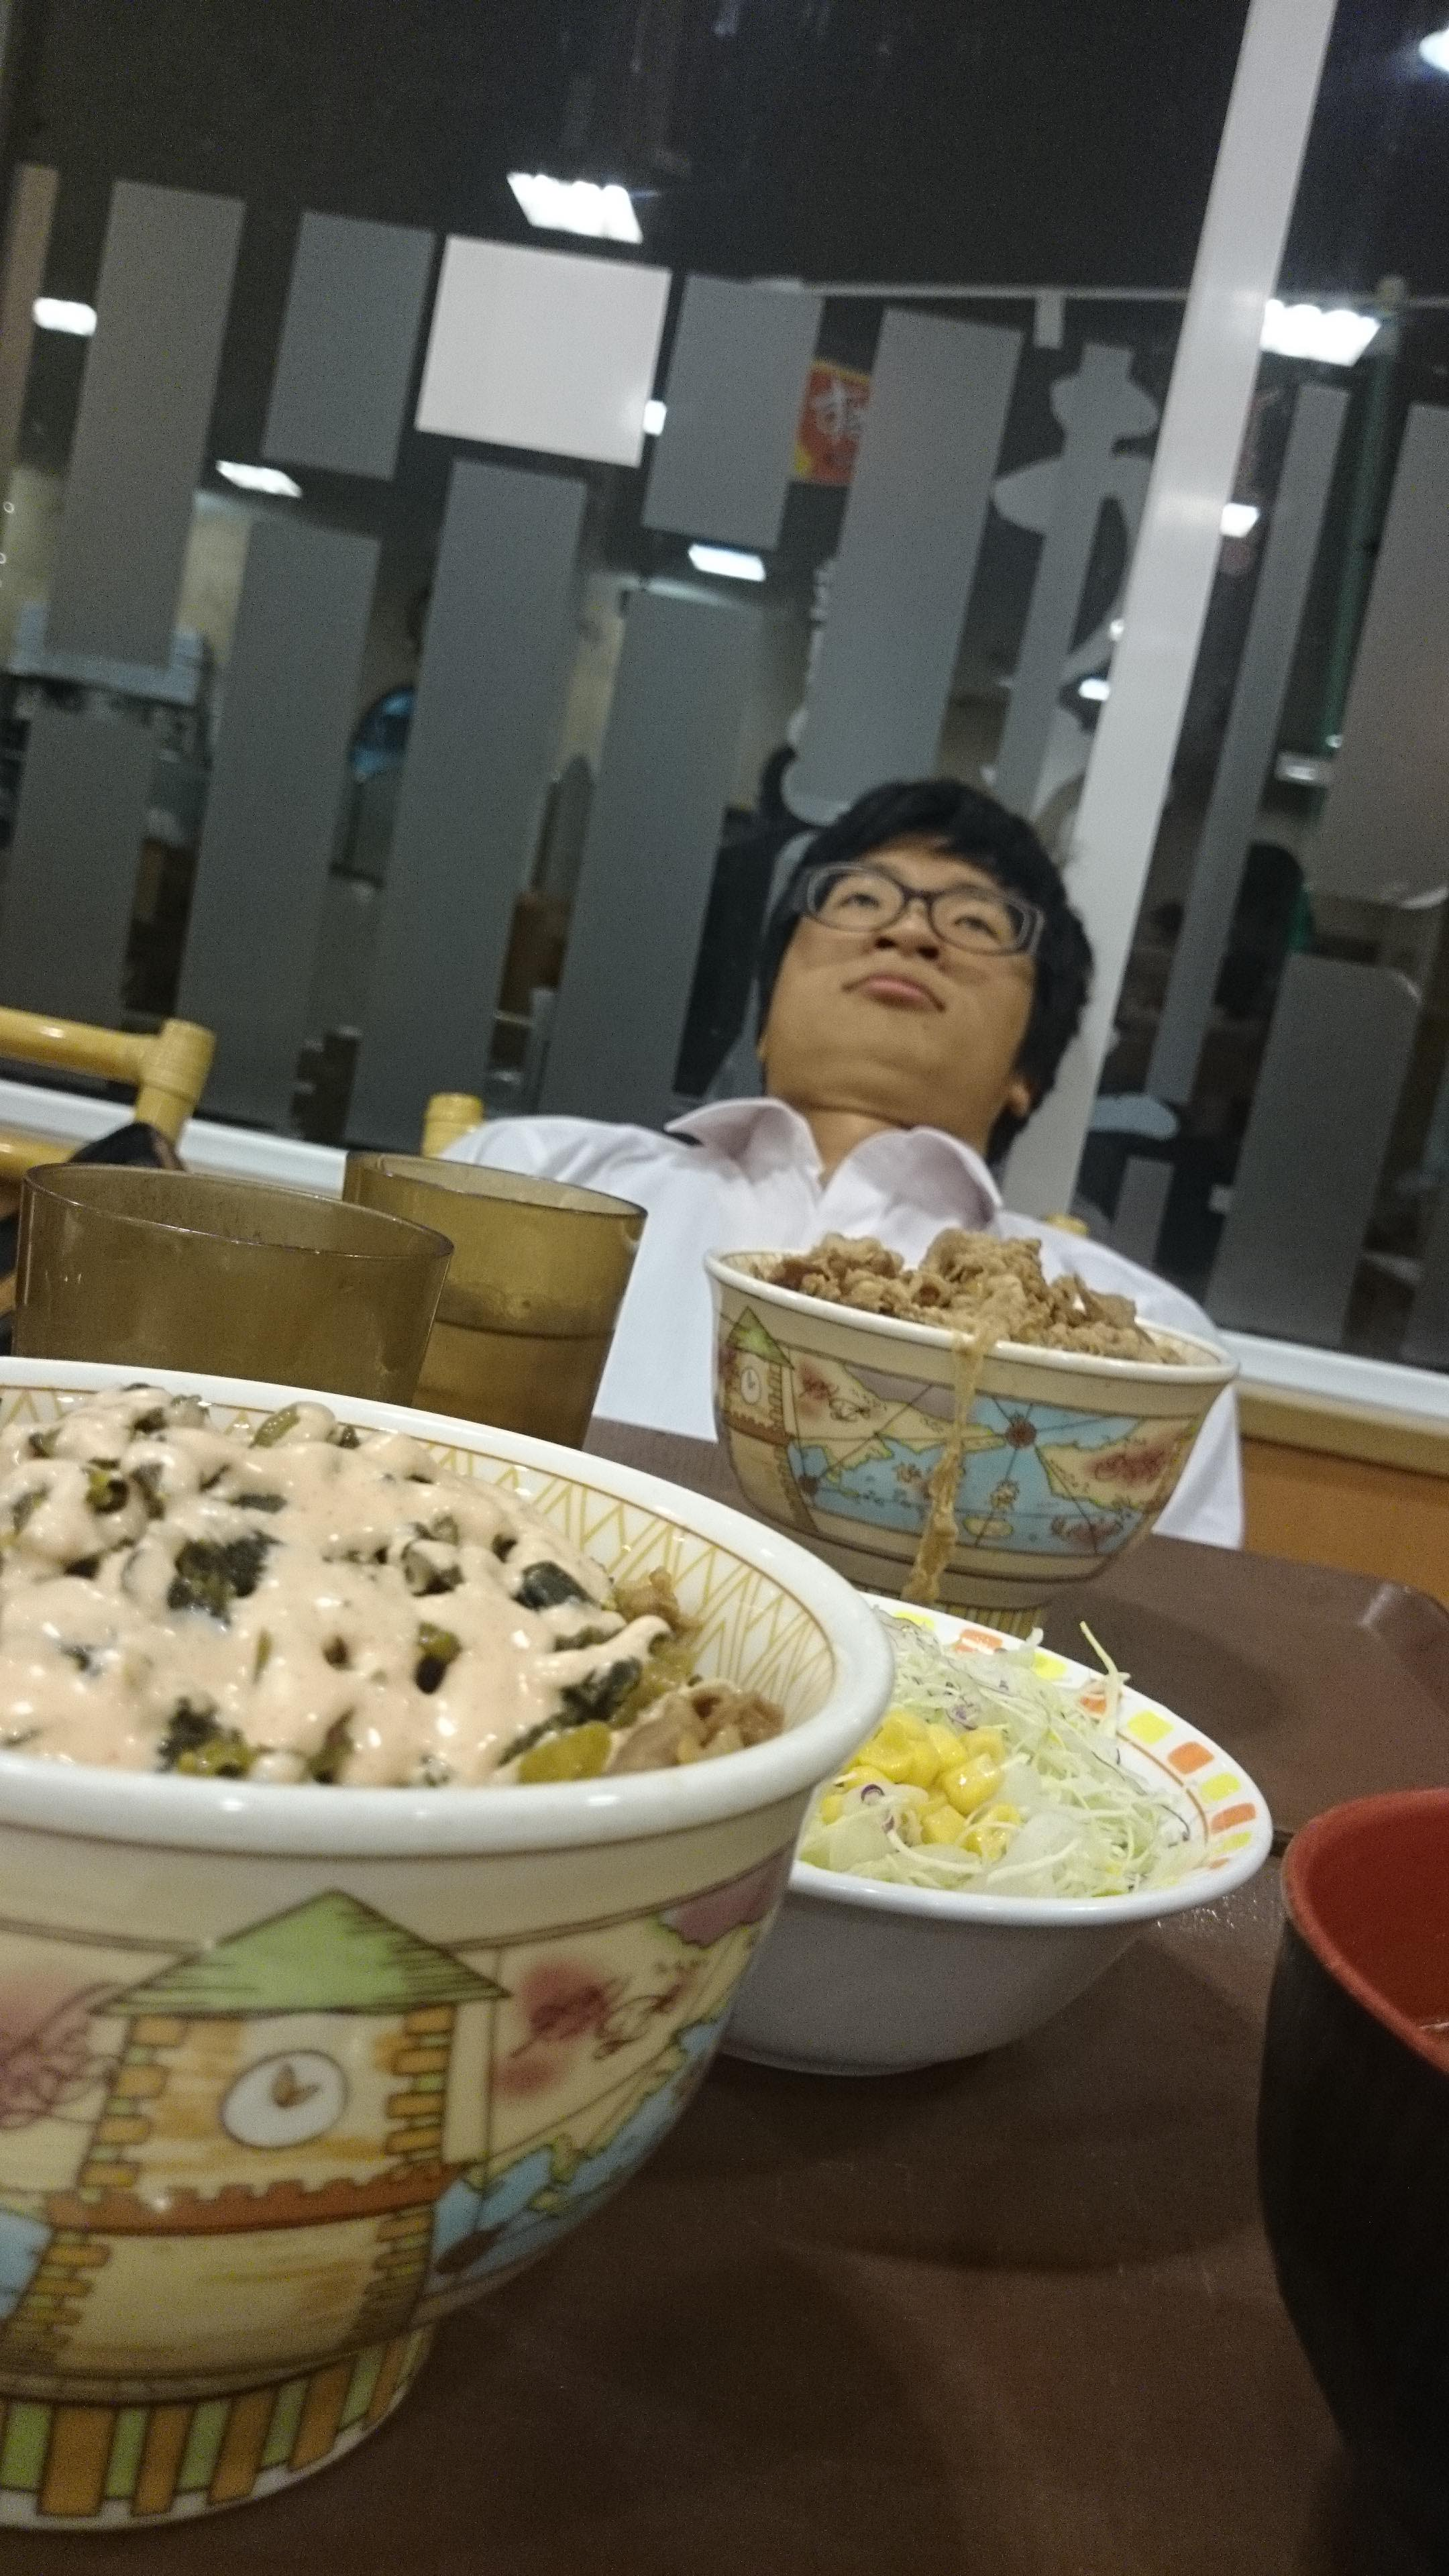
\includegraphics[width=0.3\textwidth]{./section/Shokuji/figures/LifeSukiya_3.jpg}
  \caption{図\ref{Fig:Ogawa}とはあまりにも別人の様に見える写真である。彼は今にも「バァァ」と言いたげな、物憂げな顔をしている。彼の頭の中は、時速60km/hのことで頭が一杯である(60km/hで走らないと、車線変更できず家に帰れないのである)。}
\label{Fig:OgawaBetsujin}
\end{figure}
% ----------------------------------------

%==========================%
\subsection{虎と龍}
%==========================%
また、彼らは(今は無き)虎と龍の替え玉祭りにも、バイト終わりに挑戦するという偉業を成し遂げている。
替え玉祭りとは、年に数回行われる、虎と龍の替え玉無料食べ放題キャンペーンであり、非常にお得なイベントである。
祭り素人は、バリカタであったりハリガネを頼むかもしれない。
しかし、そのような硬さを攻めていればスープは麺に持っていかれ、3玉目にはもはやスープがほぼない状態に陥ることもある。
かといって、ふつう、やわめを頼めば、1玉の体積は増えるので、これはこれで食べるのが非常に辛いのである。
そのような男の決断、英断を重ねて、ようやく5玉食いに到達できるのである。

% ----------------------------------------
\begin{figure}[h]
\centering
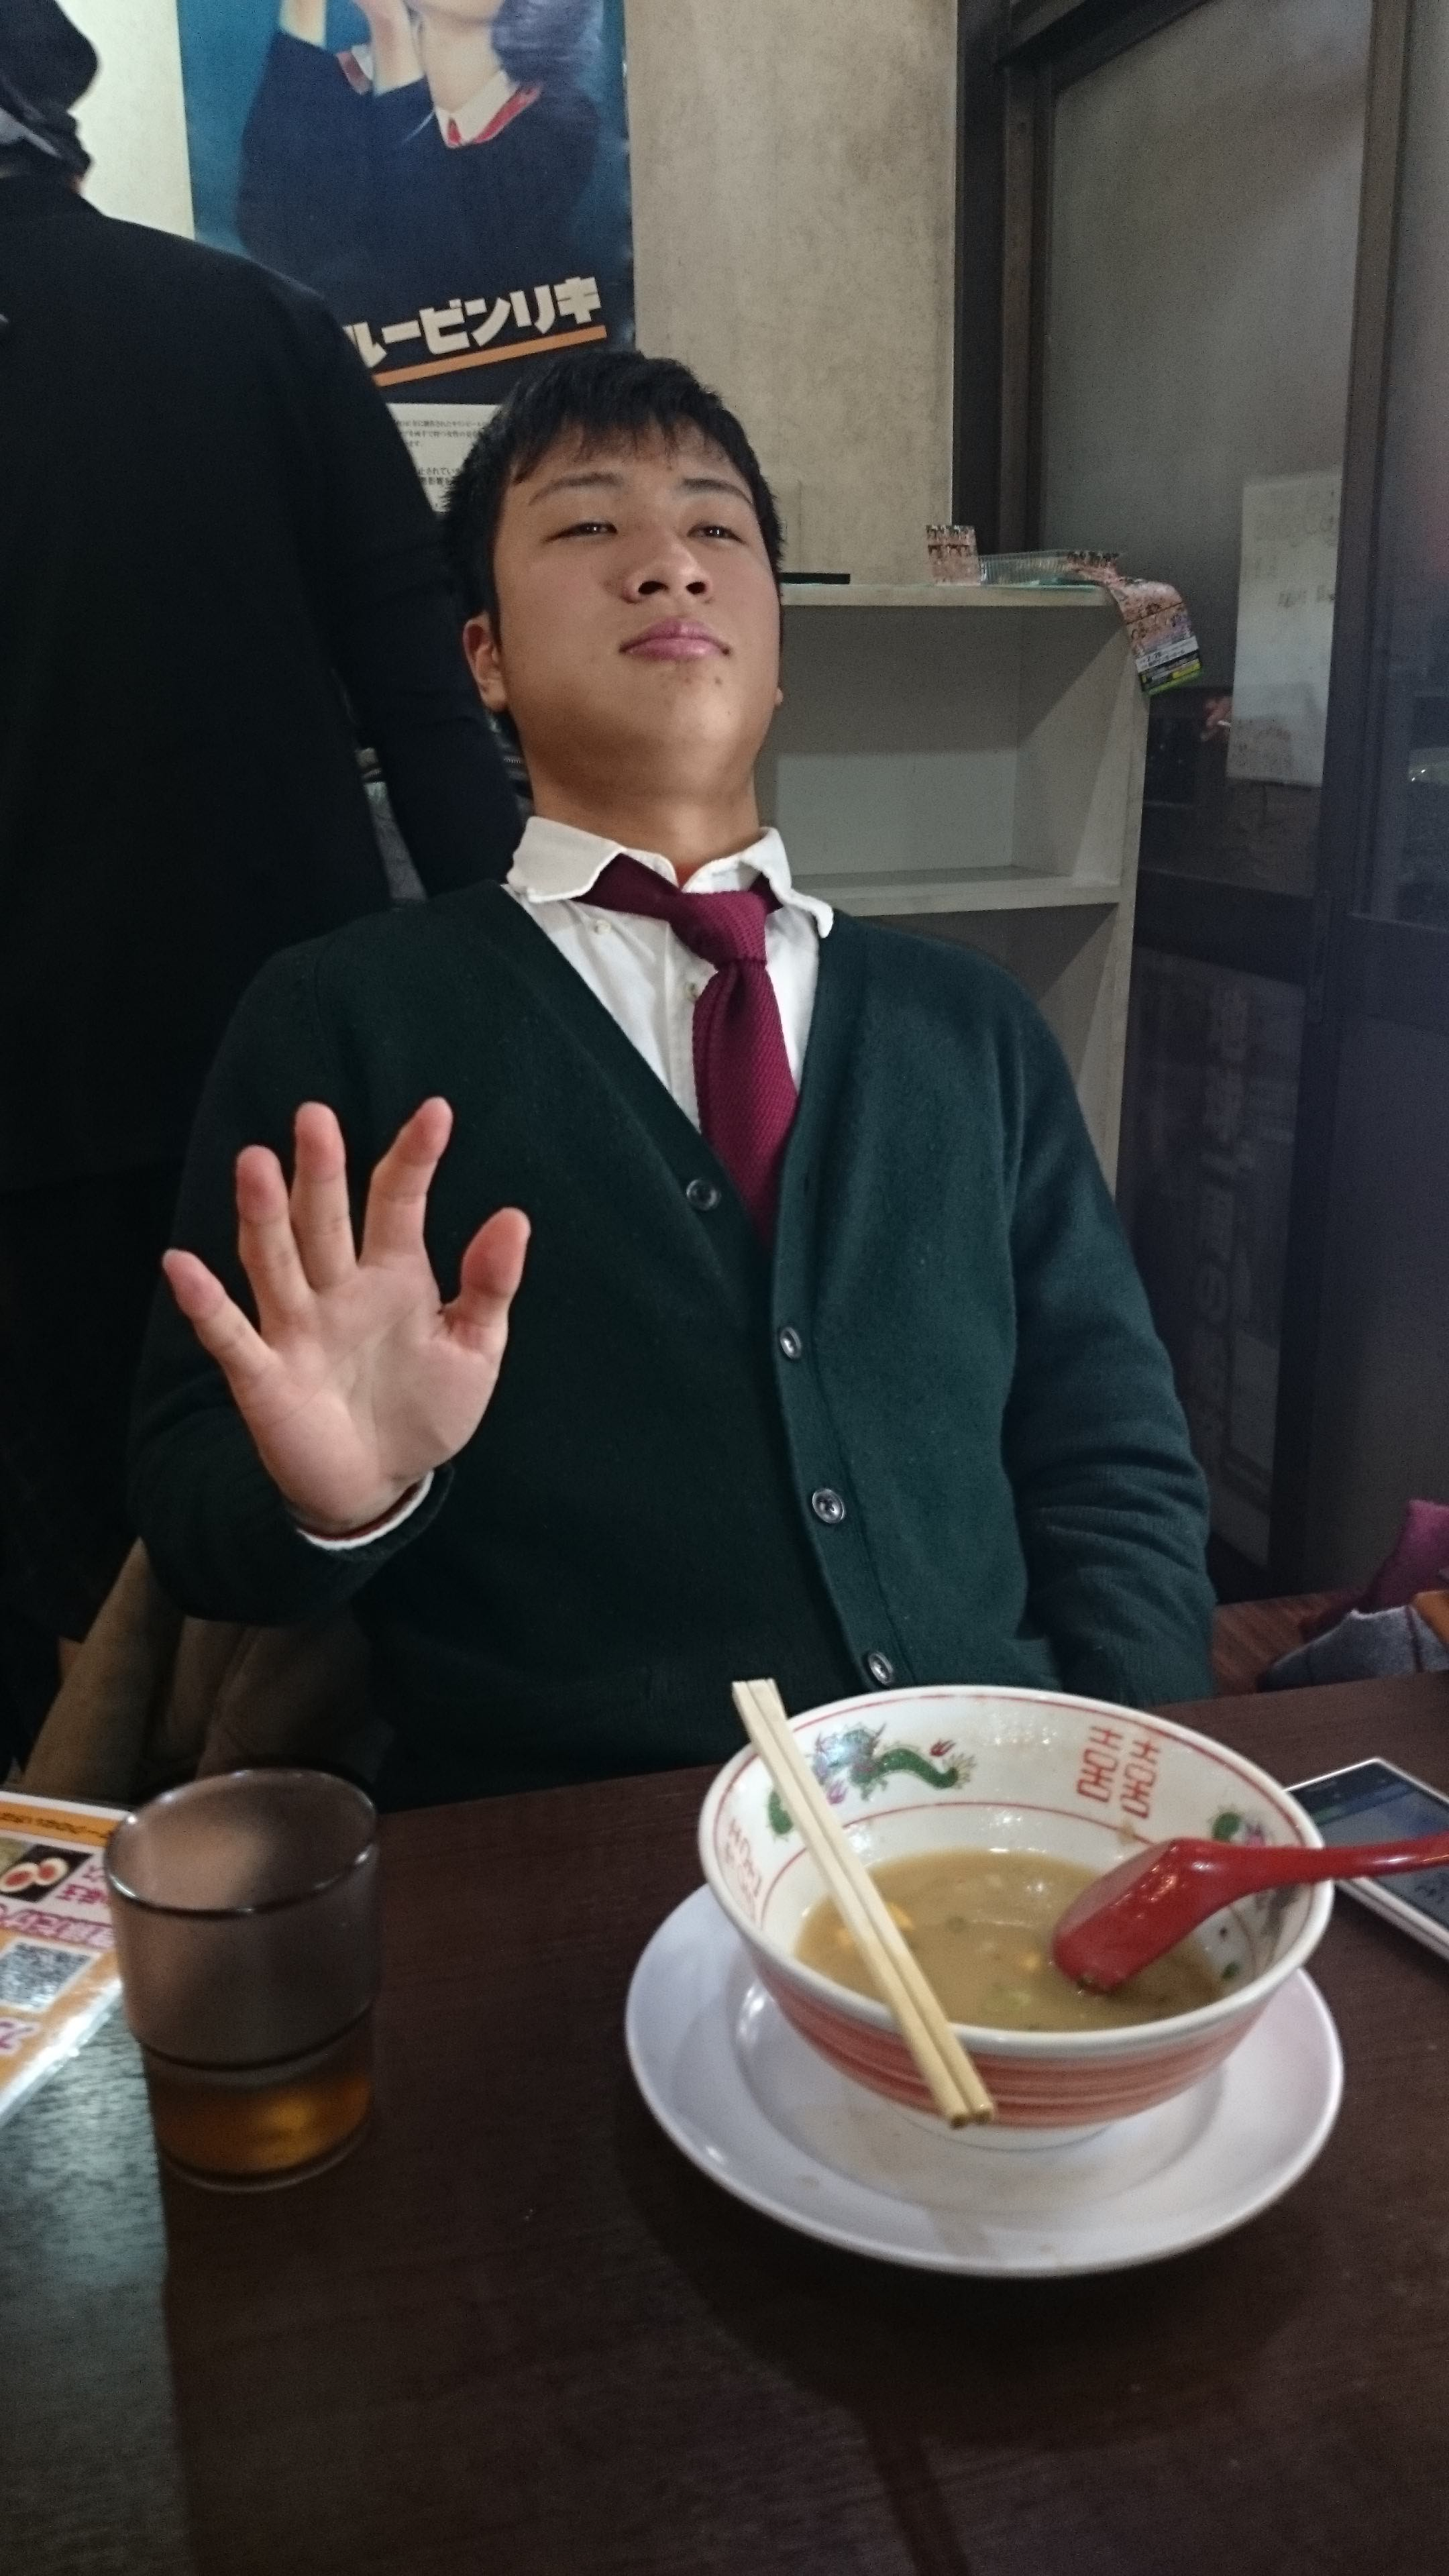
\includegraphics[width=0.3\textwidth]{./section/Shokuji/figures/Toraryuu_1.jpg}
  \caption{5玉をたいらげ、もはやギブアップ寸前のオガワ。ここから原動機付自転車を時速60km/hでぶっ飛ばし門限までに寮に帰らなければならないのである。このようにぶっ飛ばしまくり、またロクにオイル交換をしていなかったためか、晩年のオガワバイクは最高時速が40km/hに落ちることとなる。原付、晩年はエンジンかかりにくかったんやけど、晩年にマタヨととびえもん太郎とくら寿司にいく約束してて、俺だけ原付で満を持して出発しようとしたら急死して徒歩遅刻したという。そして後に、なんとか動かしつつ近所のバイク屋に持ってって、重症患者の認定を受け、廃車宣言をし、交渉の末、無料でその日に廃車が決定した。}
\label{Fig:Seiza}
\end{figure}
% ----------------------------------------

%==========================%
\subsection{ちなみに}
%==========================%
ライフオガワ店は、晩年まで「実習中」であることが知られており、
いかにライフにおける作業を体得するのに時間がかかるかが分かるであろう。

% ----------------------------------------
\begin{figure}[h]
\centering
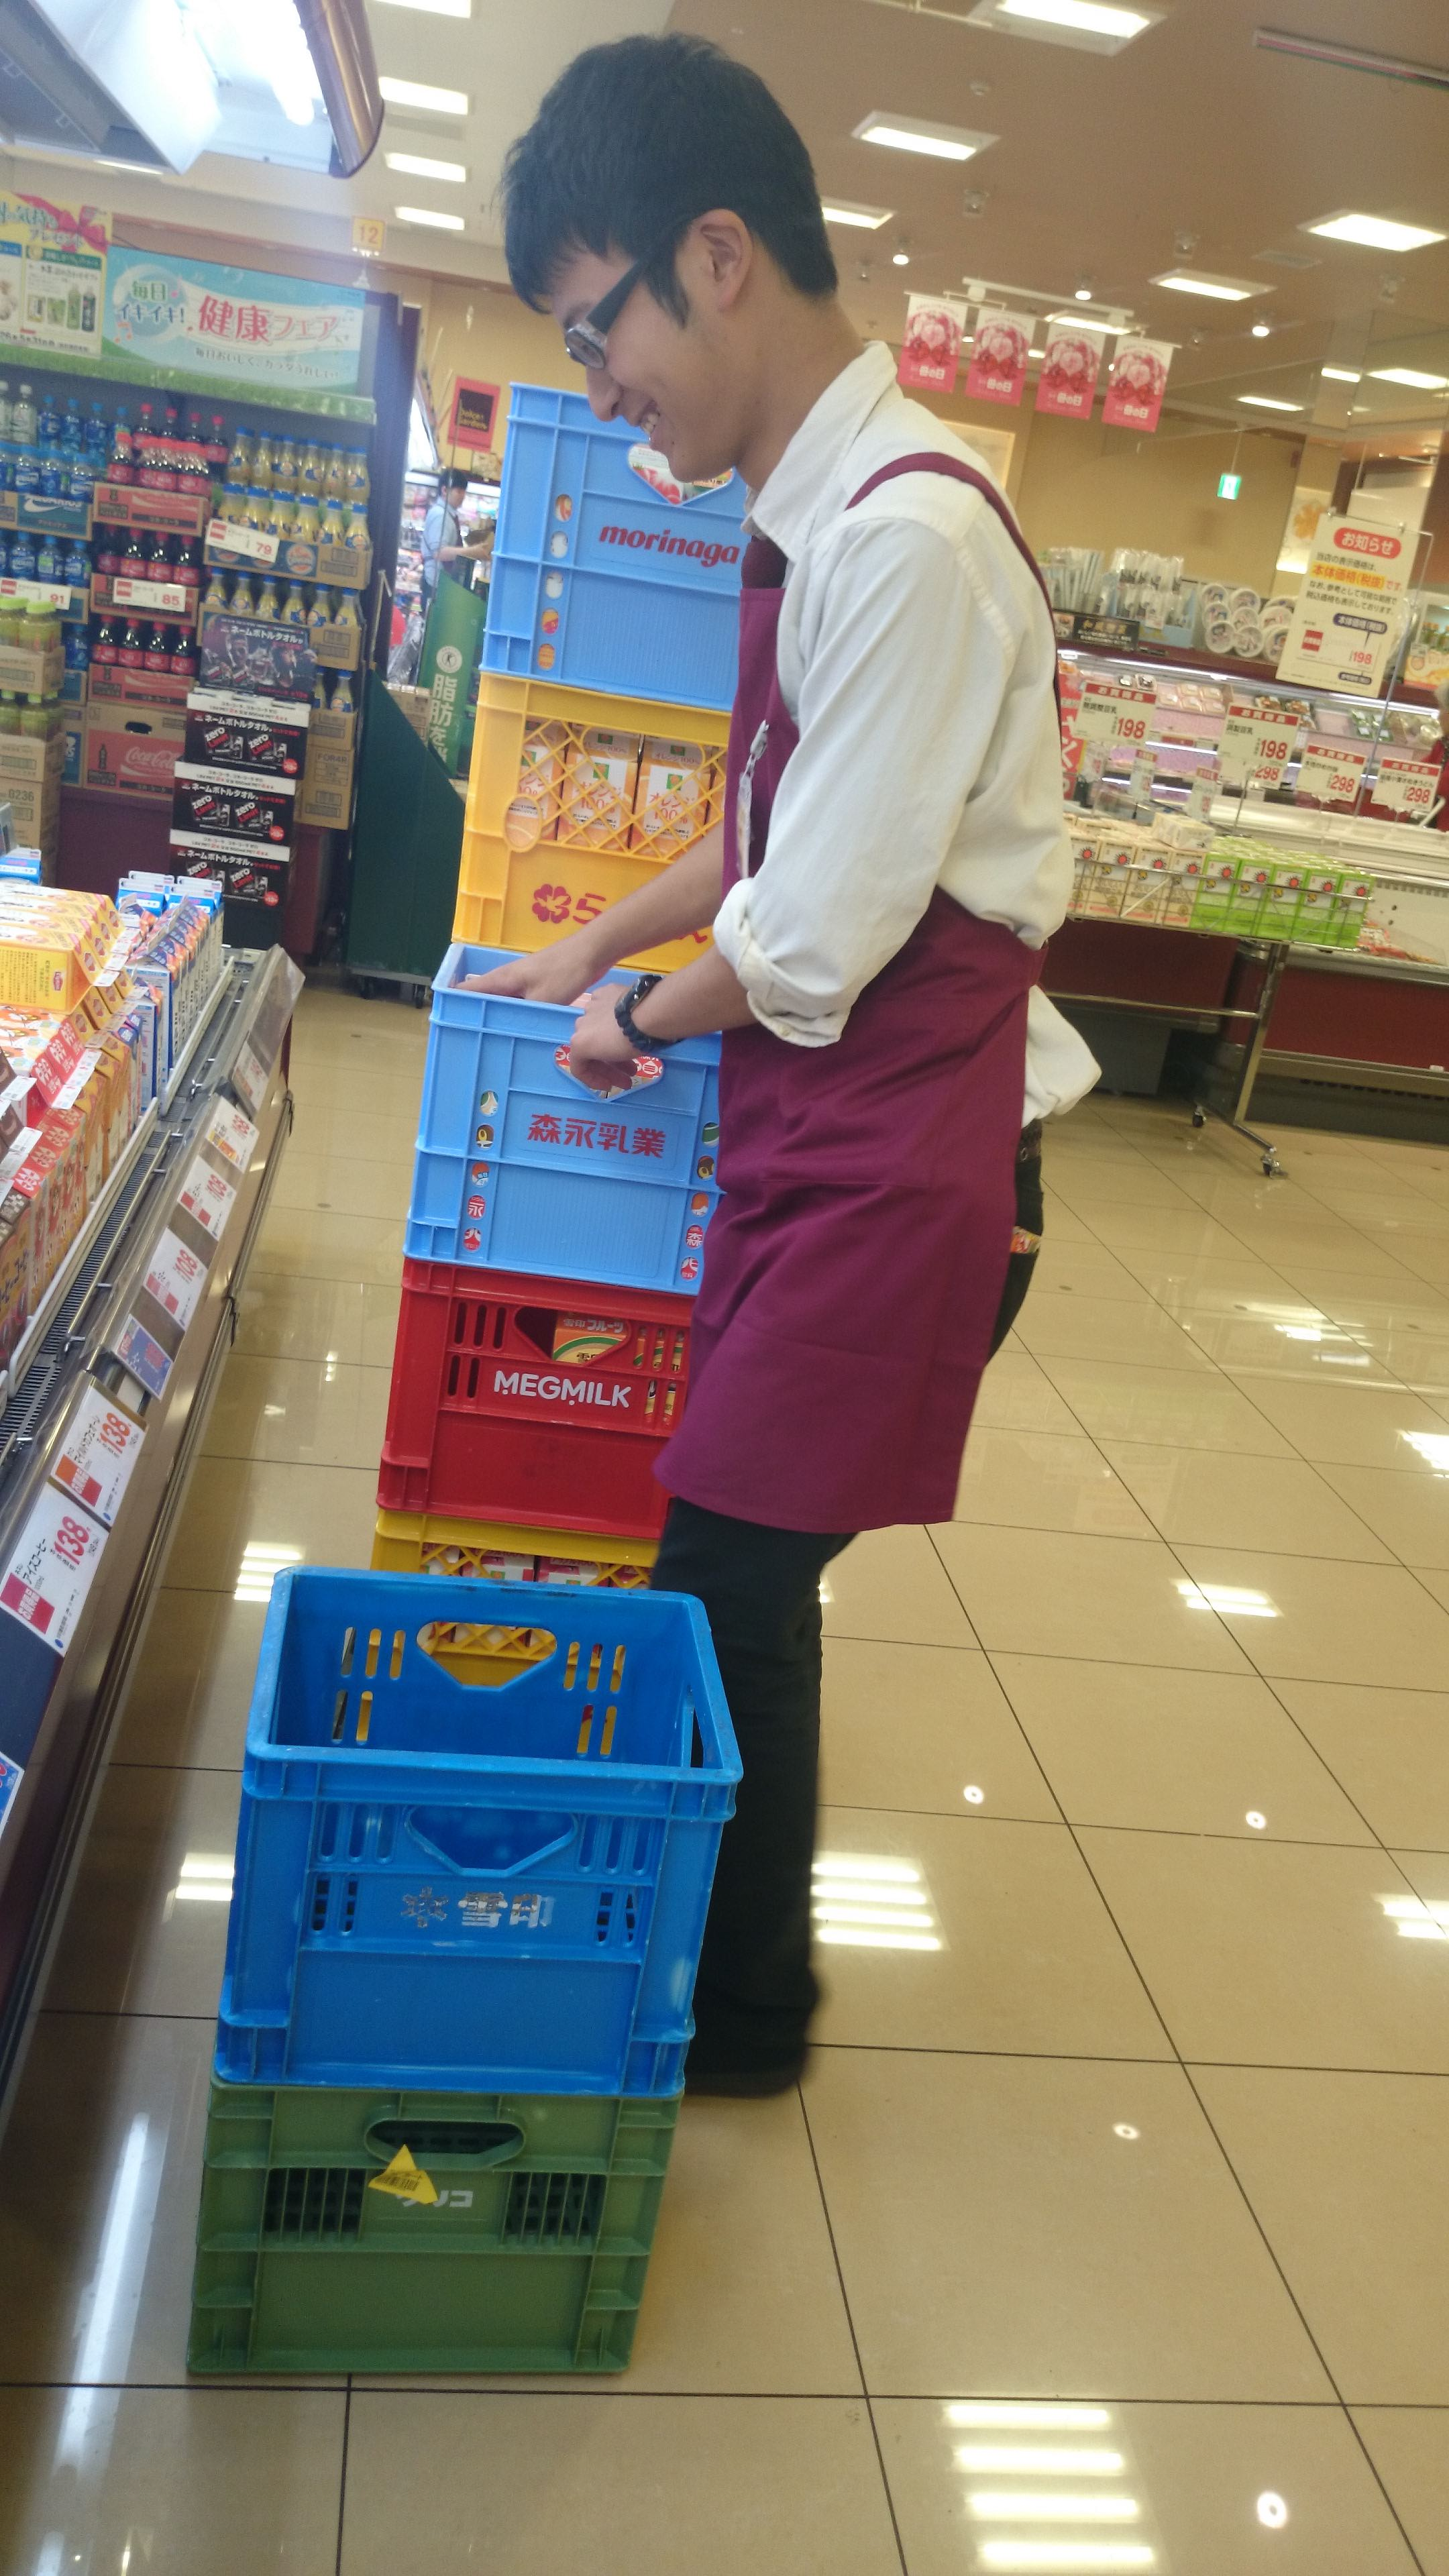
\includegraphics[width=0.3\textwidth]{./section/Shokuji/figures/Life_byte.jpg}
  \caption{バイト中の奇跡の一枚。彼は常に仕事をしつつ、パクれるものがないか品定めをしているのである。自らが欲する商品を見つけた場合、図の様に不敵な笑みを浮かべ、}
\label{Fig:Seiza}
\end{figure}
% ----------------------------------------

%%%%%%%%%%%%%%%%%%%%%%%%%%%%%%%%%%
\section{初めての阪神甲子園球場}
%%%%%%%%%%%%%%%%%%%%%%%%%%%%%%%%%%
ライフでの勤務により、超越した晩御飯を経験する回数が非常に増えたわけであるが、
食事だけでなく睡眠時間さえも通常の睡眠を超越した日があった。
それが、甲子園球場殴り込みの日である。
彼らはライフでの勤務が終わると(ごくたまにレジを悪用し、半額祭りを行っていたのだが)、双眼鏡を購入するためにドン・キホーテへと駆け込んだ。
そして一旦家へ帰り、仮眠を取る。
翌朝3時に起床し、始発で甲子園駅に行くためである。

\subsection{阪神甲子園球場}
甲子園駅に付いたものの、降車する人の先頭をきって動くことになってしまったため、全くどちらへ行ってよいか分からない彼らにとって、特に方向に感度を持たない特定の人物にとって、非常に困惑した事態となった。
標識もロクにでていないため、なんとなくで向かっていき正しいことが分かると、やがて、早足になり最後には駆け足で、入場の列へと殴り込むことになる。

% ----------------------------------------
\begin{figure}[h]
\centering
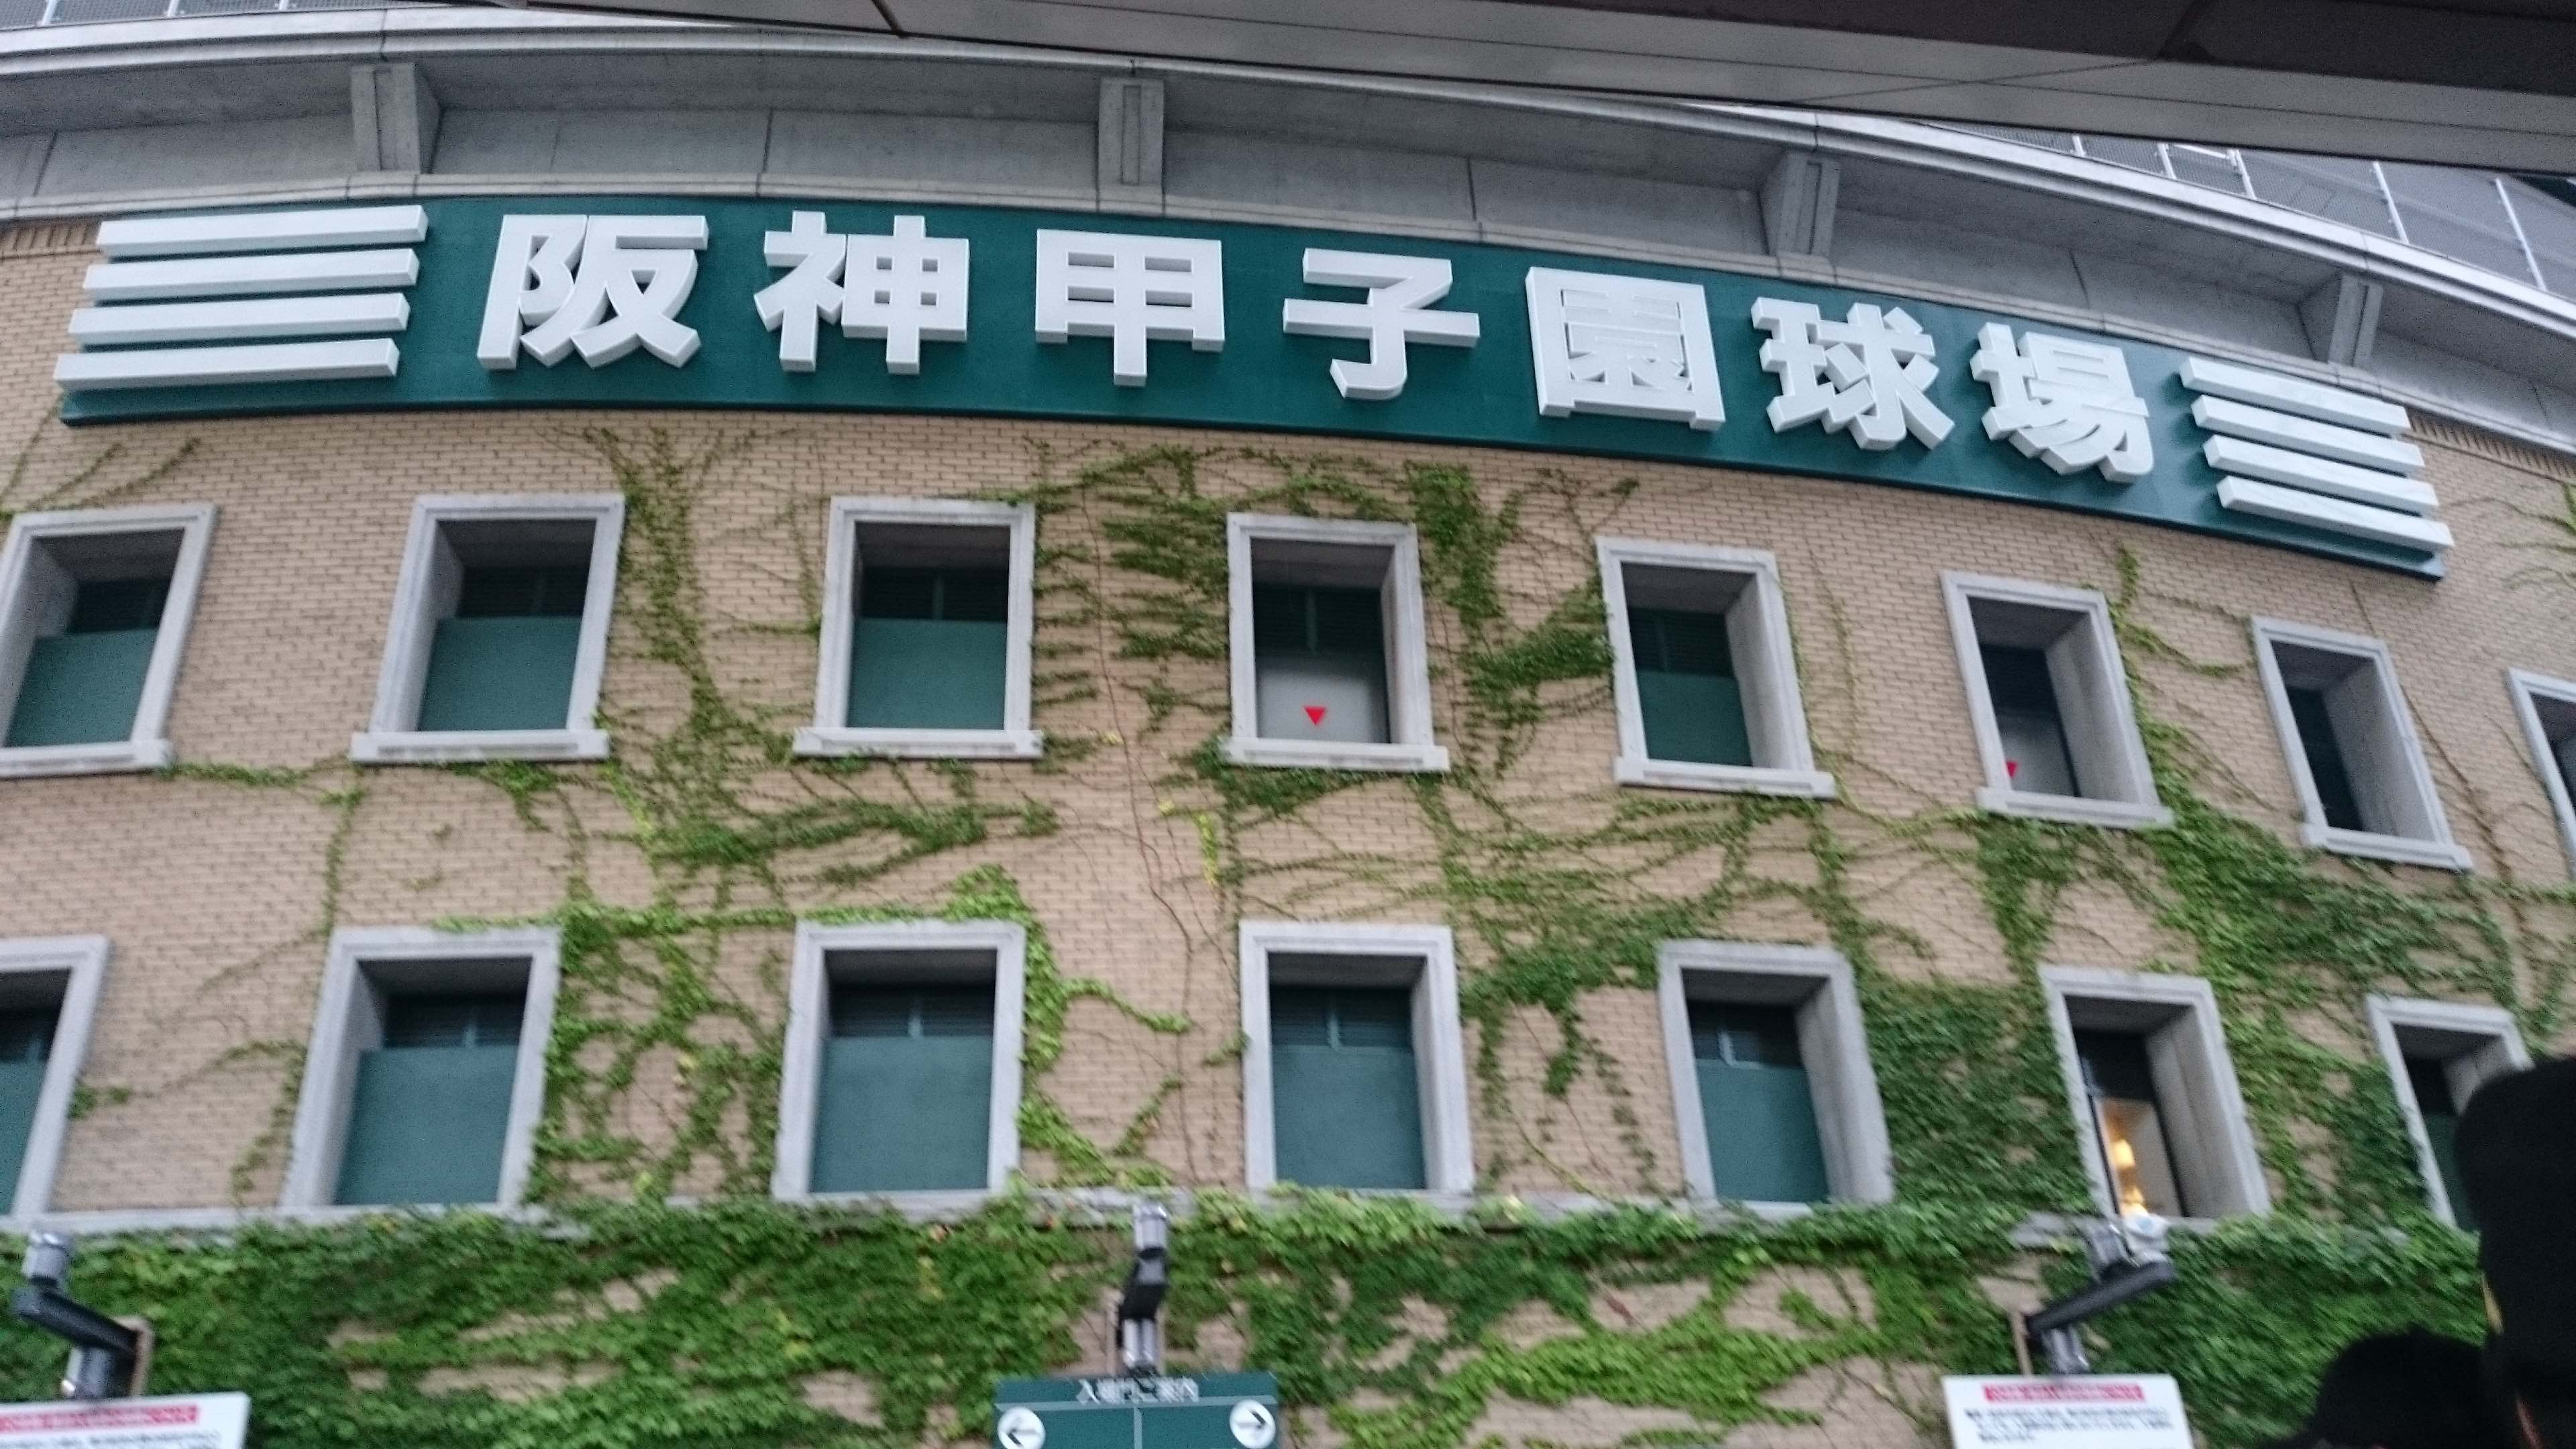
\includegraphics[width=0.7\textwidth]{./section/Shokuji/figures/Koushien_1.jpg}
  \caption{ついに見えた阪神甲子園球場。これから殴り込みに行くのである。}
\label{Fig:Seiza}
\end{figure}
% ----------------------------------------



\subsection{朝食という概念}
早朝3時に起きたため、もちろん到着した段階でお腹が空いており、近くのマクドナルドで朝マック持ち帰りを行うこととした。


% ----------------------------------------
\begin{figure}[h]
\centering
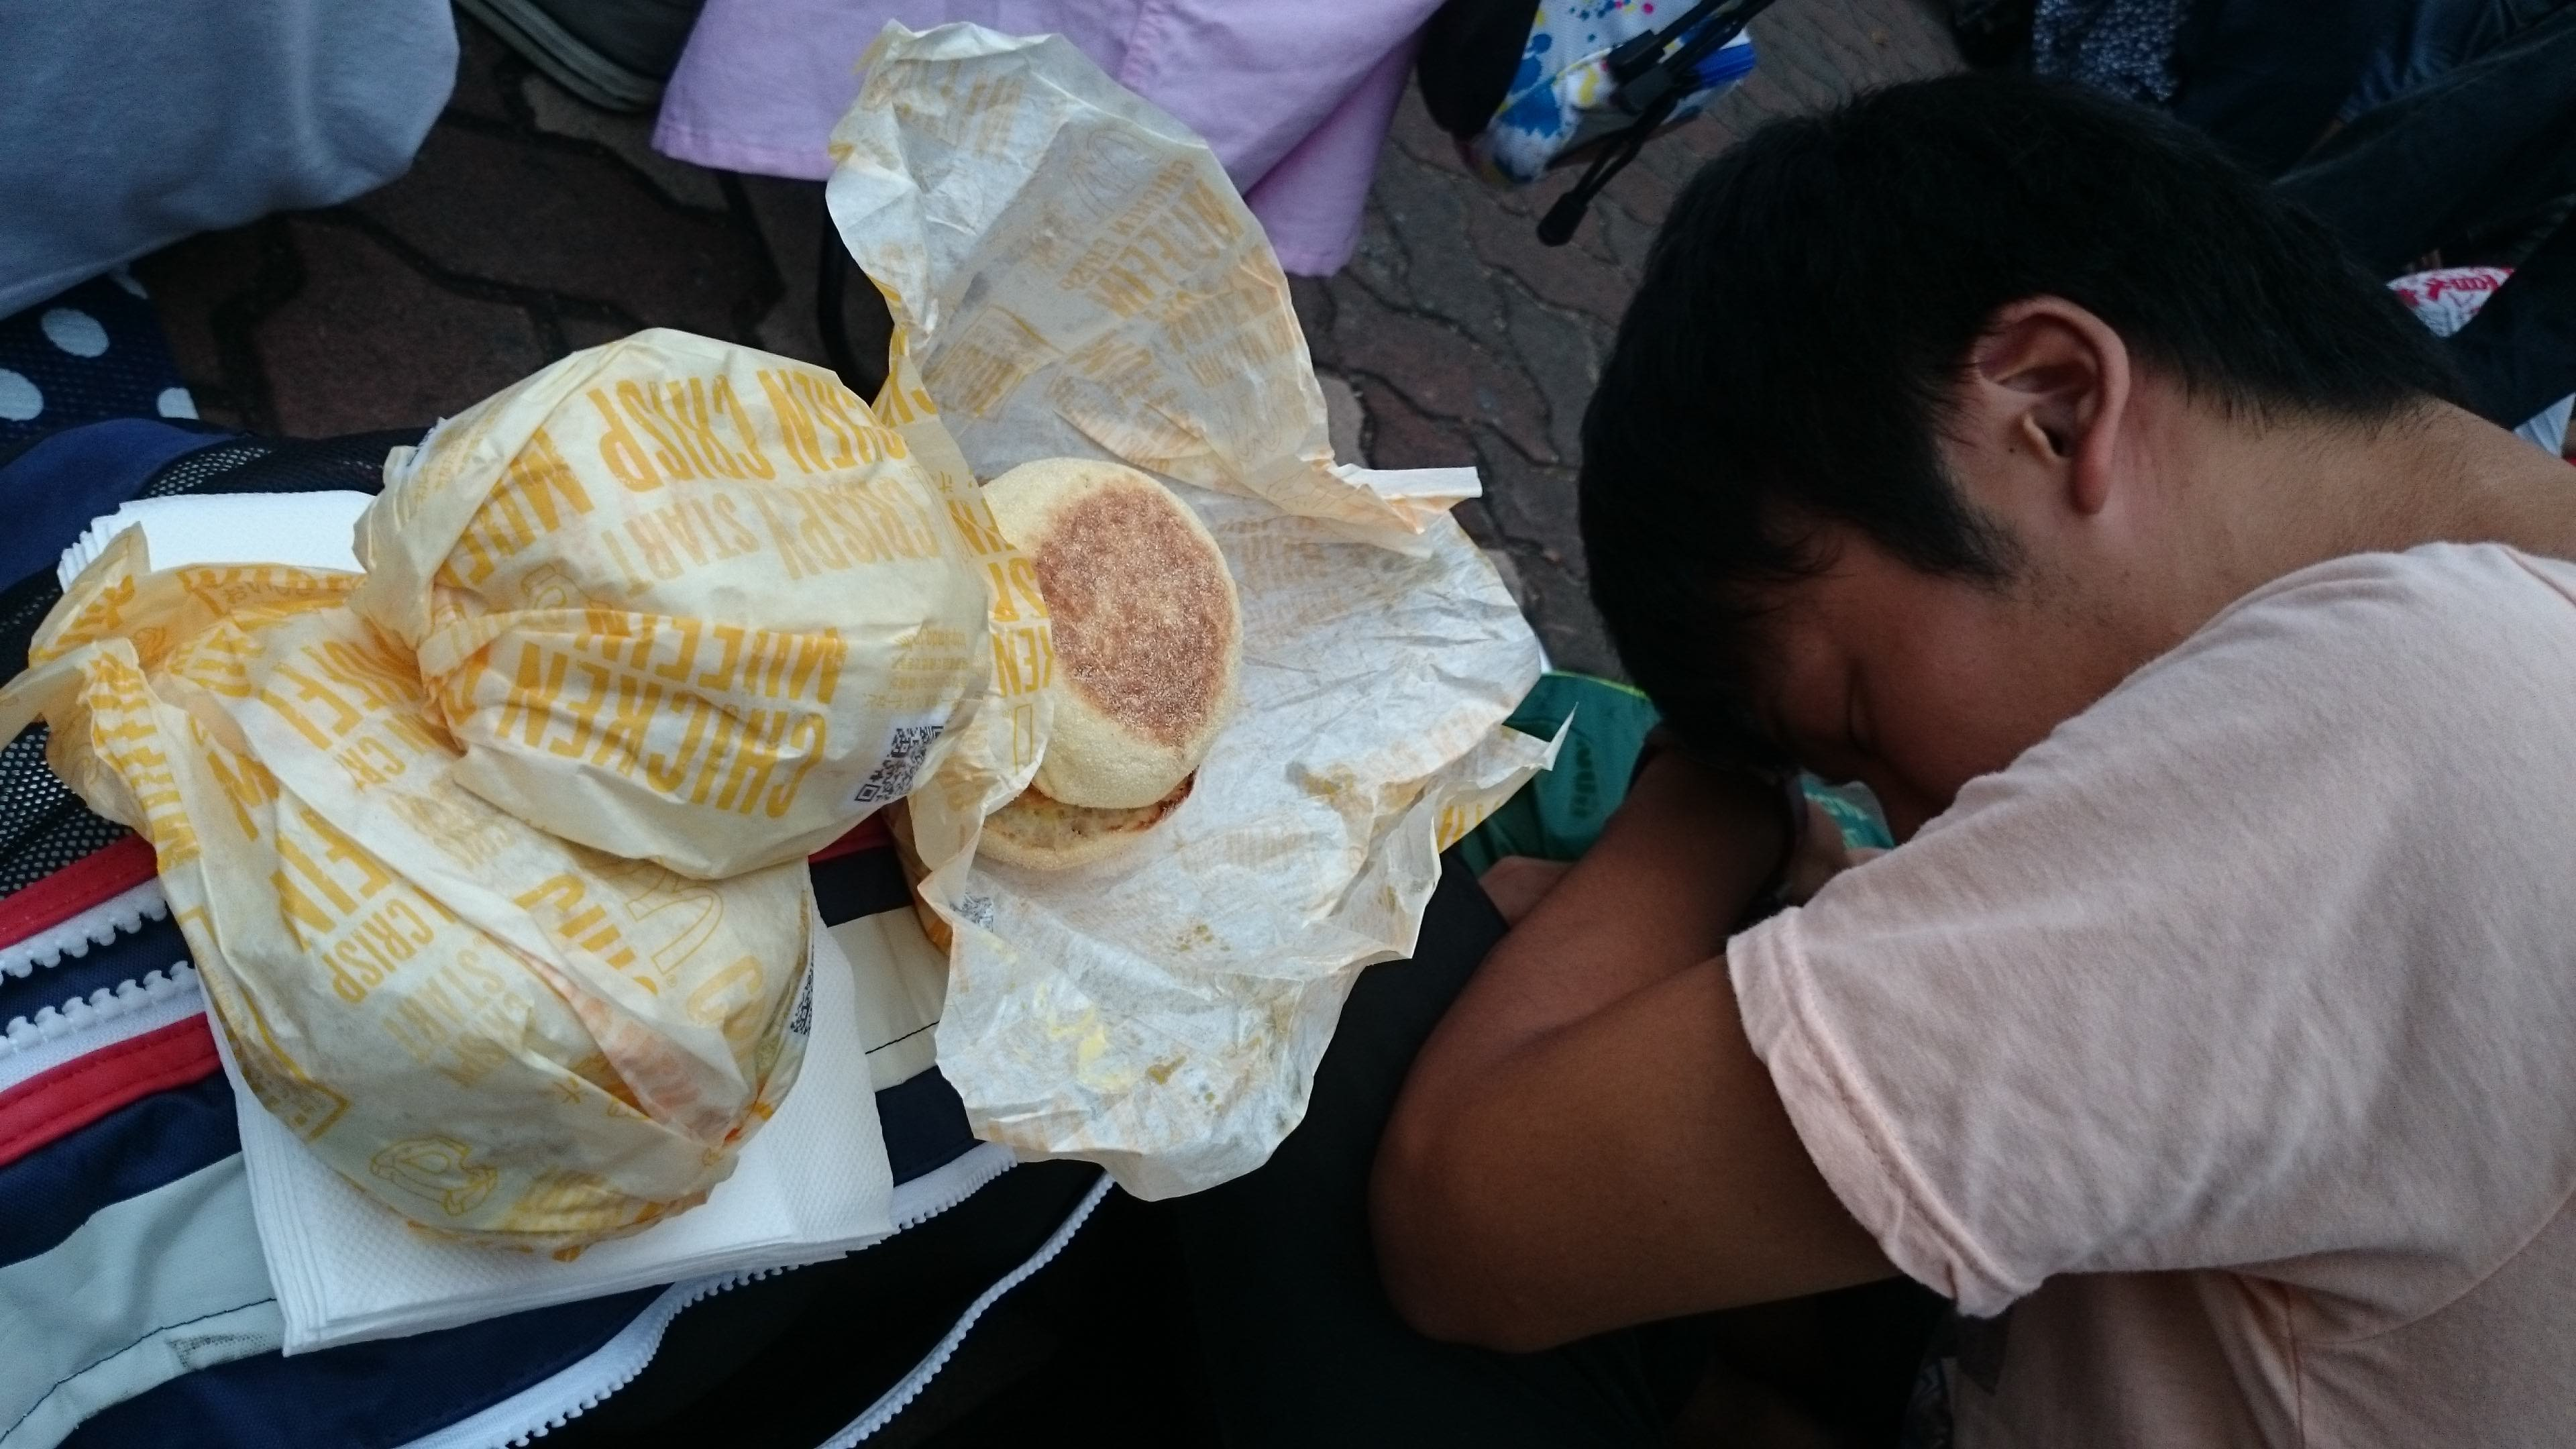
\includegraphics[width=0.7\textwidth]{./section/Shokuji/figures/Koushien_breakfast.jpg}
  \caption{持ち帰ってきた朝マックたち。彼は既に死んでいる。}
\label{Fig:Seiza}
\end{figure}
% ----------------------------------------


\subsection{殴り込みに当日の対戦カード}
野球をよく分からない人間でも知っている高校が出場しているので、たぶん良い日なのだろう。
たしか、この日の夕方にも何故かバイトを入れていたので、途中で早退したのであるが。

% ----------------------------------------
\begin{figure}[h]
\centering
\includegraphics[width=0.7\textwidth]{./section/Shokuji/figures/Koushien_2.jpg}
  \caption{本日の三塁側のチーム}
\label{Fig:Seiza}
\end{figure}
% ----------------------------------------

% ----------------------------------------
\begin{figure}[h]
\centering
\includegraphics[width=0.7\textwidth]{./section/Shokuji/figures/Koushien_3.jpg}
  \caption{本日の一塁側のチーム}
\label{Fig:Seiza}
\end{figure}
% ----------------------------------------

\subsection{殴り込み}
いざ球場に入ると、感動もひとしお。しかし彼らの目的は、野球を楽しむことではなく、殴り込みに行くことであったので、オガワ氏は殴り込もうと思った。
その矢先、市民は恐れをなしてオガワ氏から逃げていくではないか!

% ----------------------------------------
\begin{figure}[h]
\centering
\includegraphics[width=0.7\textwidth]{./section/Shokuji/figures/Koushien_4.jpg}
  \caption{こちらを向き、たたずむ小川青年。}
\label{Fig:Seiza}
\end{figure}
% ----------------------------------------




%%%%%%%%%%%%%%%%%%%%%%%%%%%%%%%
\section{なんやこれ}
%%%%%%%%%%%%%%%%%%%%%%%%%%%%%%%
人生勝ち組の男が、こちらを睨んでいる。
武田学長の権力を持ってさえも、クビにすることはできない。
民主党政権時の、スーパーコンピューターの予算を削る時に、この男も削られればよかったのである。

% ----------------------------------------
\begin{figure}[h]
\centering
\includegraphics[width=0.4\textwidth]{./section/Shokuji/figures/Nanyakore.jpg}
  \caption{見方を変えれば人生勝ち組の助教授。床で寝てるだけで年収数百万円なのだから。}
\label{Fig:Seiza}
\end{figure}
% ----------------------------------------


\subsection{オガワ・バイク・オガワ(OBO)}
オガワは、学長に就任して以来、経営危機にあった非言語大学をV字回復させた。
さらに、ルノーや三菱自動車の会長も兼務した、世界的なカリスマ経営者として伝説に残っている。
このような経営改革を行ってきた、オガワ学長がどのような人生を送ってきたか、機構長の観点から簡単に紹介する。

\begin{figure}[h]
\centering
\includegraphics[width=0.8\textwidth]{./section/HigengoUniv/figures/DSC_0113_2.jpg}
\caption{盗んだバイクで走り出す。学長と言えど、犯罪はおかすし、バイクで転ぶ。}
\end{figure}


%記憶の最初は、ヨネヨネCLUB創設である。
%阪急電車十三駅で特急に乗り換えているときに「Wikipediaでリンクを辿っていけば絶対に自分の行きたいページにいける」というネタをひっさげてお互い喋っていた。
%そのときに初代機構長が「こういうネタあるよ、小川くんの好きなものはなに?」という答えに対し「EXILE」であると答えたことが未だに記憶に残っている。
%案の定、任意のページからEXILEに辿り着き、まぁまぁ初対面ながら間がもったのは覚えている。



%%========================%
%\subsection{LIFE的観点}
%%========================%
%\begin{figure}
%\centering
%\includegraphics[scale=0.1]{./section/HigengoUniv/figures/DebuKatsu.jpg}
%\caption{ライフ近くの晩ごはん屋さん。}
%\label{mimi}
%\end{figure}


%学部生3回生の頃の初代機構長はバイト先に困っていた。
%そのところに、小川総務大臣の助言によりライフで働くことになった。なんとなくレジに興味あると言って、なんとなくレジ部門になった。半額ボタンを押して色々買ったり、買い物に来た宮崎大輔のコメを半額にしてやった。ある程度してやめた。
%ここから俗に言うデブ活が更に加速していったのである。



%\subsection{建立(ケンリツ)}
%非言語革命により設立された非言語大学であるが、特に初代機構長は様々な新歓を渡り歩き、初代総務大臣はCSC(?)を渡り歩いていた。







%%%オガワマン登校分布
%======================
\chapter{オガワマン登校分布}
%======================

重症患者には様々な爆誕方法が存在する。特に、研究室に登校する際の爆誕方法を示す表現方法は多種多様であり、目を見張るものがある。本章では、世界各地で用いられているその表現方法についてまとめる。
%==================
\section{そもそも「登校する?」という概念}
基本的に、各々の重症患者がサークルや部活、バイトや授業、竹田徹夜などで普段から生活リズムがバラバラバラバラ\footnotetext{$\sf{ (´\_ゝ`)}$バラッッッッッッッッ}である。そこで、その日にお互いが登校するかどうかを把握する上で非言語予定確認という観点から「登校する?」という概念が生まれた。たぶん。\\
 特に、オガワマンは不定期に研究室に来なくなったりするため、日々のオガワマン登校の確認という概念の分布、いわば概念分布の研究が進められた。今回は、凄腕の研究期間であるJAXA (Japan Abaponnu X-ray Abaponnu)の研究結果を示す。
\begin{figure}[H]
\centering
\includegraphics[clip,scale=0.25]{bara.jpg}
\caption{まあLINEでどんな非言語パスが来てもこれよりはマシやから何も思わない$\sf{ (´\_ゝ`)}$}
\label{bara}
\end{figure}

\section{オガワマン登校分布}
まあ一覧にするだけやけど$\sf{ (´\_ゝ`)}$笑\\
 以下は全て「登校する?」という意味である。おそらく。

\begin{itemize}
\item 生える?
\item 存在する?
\item 来る?
\item 死亡?
\item 生えてる?
\item いつ生えんの?
\item 行くべき?
\item マンゴスチン栽培は今日は無し?
\item 寿命は?
\item いま研究室?
\item 登校ポコ
\item 胃袋は?
\item きょうは農地耕作なし?
\item 剃られた?
\item 生えわたる?
\item 明日生える?→剛毛育毛剤→バンドロポン
\item ホッタイモ今日生えわたる梅酒ソーダ割り?
\item 芋掘ってる?
\item Mn登校は?(→まさか金八?)
\item ヒゲバーストに便乗して、オマンゲン寺から一時出家(→まだ入ってる?)
\item 存在?
\item 生きてる?
\item 生えまくり?
\item 梅酒?
\end{itemize}

%%%ウンコ原理
%!TEX root = ../../main.tex
\chapter{ウン・コ原理}
そもそも原理とは、それ自体は他に依存せず、他のものがそれに由来するような始りのことをいう。
とくに、自然科学においてはある理論体系の基礎になっている法則および命題をさす。
つまりそれ自体は証明することが困難であるが、その他の実験結果から正しさが証明されているため、それ自身も自身も正しいとして考えられているのが、原理である。
以上で一般的な「原理」を定義したわけであるが、ここではもう一つ踏み込み、自然科学を超越した理論体系として脚光を浴びている理論が準拠するウン・コ原理について導入し、その正しさを証明し実際にそれ自身が原理であることを確認し結論とする。

\section{日本における祝日}
そもそも日本における祝日は、昭和23年に施行された祝日法によって定められており、祝日法に従い全16日の祝日が定められている。
その中でウン・コ原理を完全に理解するためには、日本における元旦に対する正しい理解が必須となる。
元旦とは、祝日法によれば「年のはじめを祝う」とされており、戦前は元旦の早朝に天皇陛下が行っていた四方拝という祭祀に基づいて「四方節」と呼ばれていた。
この様に元日を気持ちよく迎えることは、その一年を占うことになる、と一般的に考えられている。

\section{始まりの一言}
そのような元日に始まりの一言が発せられた。
\[
ちなみにうんこ餅は忘れてた。
\]
これが今後の自然科学を超越した理論構築の根拠となる、ウン・コ原理発見のきっかけとなった一言である。
まず、図\ref{Fig:UnkoGenri}を見ていただきたい。

% ----------------------------------------
\begin{figure}[htbp]
\begin{center}
 \begin{minipage}{0.7\hsize}
  \begin{center}
\includegraphics[width=0.5\textwidth]{./section/UnkoGenri/figure/Unko1.png}
  \end{center}
  \label{fig:one}
 \end{minipage}
 \begin{minipage}{0.7\hsize}
  \begin{center}
\includegraphics[width=0.5\textwidth]{./section/UnkoGenri/figure/Unko2.png}
  \end{center}
 \end{minipage}
 \caption{元旦にウンコに関する発言をする議事録。ここで緑色の発言を行っている人物はタケダであり、またその会話相手は神戸大学生に絶大な人気を誇るラーメン屋である希望新風六甲道店である。}
  \label{Fig:Unkogenri}
\end{center}
\end{figure}
% ----------------------------------------

どうやら彼らは、餅についての会話を行おうとしていた様である。
しかし、一つの疑問が残る。ここでいう「うんこ餅」とは一体何を示しているのであろうか?
ここではこれ以上に情報がなく、追求することができない。
そのため、本章の議題である「ウン・コ原理」を導入することで、これらの説明を試みる。

%====================
\section{うんこ餅}
%====================
うんこ、とは一般的には図\ref{Fig:Unko}に示すような形状をしていると考えられている。
つまり、この文脈における「うんこ」とは三段巻きで形成された物体であると簡潔に定義することができる。
また「餅」とは、一般的にはお正月に頂くものであるため、これらを踏まえると「うんこ餅」とは、三段巻きの餅、つまり鏡餅(図\ref{fig:KagamiMochi})を表していると考えられる。
しかし、「うんこ餅」が「鏡餅」であることはこの文脈から判断することができないため、一種の原理を導入せざるを得ない。
これが「ウン・コ原理」である。

\begin{figure}[htbp]
\begin{center}
\includegraphics[width=0.4\textwidth]{./section/UnkoGenri/figure/Unko.jpg}
  \label{fig:Unko}
  \caption{にこやかに微笑むウンコの一例。三段巻きの構造を持っており、流されないように・捨てられないように、人へ微笑みかけていると考えられている。}
\end{center}
\end{figure}

\begin{figure}[htbp]
\begin{center}
\includegraphics[width=0.4\textwidth]{./section/UnkoGenri/figure/KagamiMochi.jpg}
  \label{fig:KagamiMochi}
  \caption{一般的にお正月に飾られる鏡餅の一例。一般的に、鏡餅は、丸い餅を二段重ねにした構造を持っている。
これは、神様のチカラが宿ったとされる青銅でできた円形の銅鏡を模しているからである。
また、二段重ねの構造は、月と太陽、陰と陽を表していて、円満に年を重ねるという意味が込められており、「福と徳」が重なるようにという願いが込められていると考えられている。}
\end{center}
\end{figure}

%====================
\section{ウン・コ原理の帰結}
%====================
この様に、「うんこ餅」を説明するために導入されたウン・コ原理であるが、本原理を用いることで更に重要な帰結を得ることができる。
それが
\[
オガワ(餅糞)マン
\]
である。
ウン・コ原理は「うんこ餅」、つまり「糞餅」を説明することができ、それの購入を忘れたオガワマンは上記のように表記することができるのである。
しかし最も重要な事実は、オガワマンは最初から購入する意思など持っていなかったのである。
この「購入する意思」を説明するためには、ライフ原理を導入する必要があり、これは本論文の範疇を大きく超えるため、ここでは割愛する。

%%% 小川万葉集
\section{小川男葉集}
\subsection{小川男葉集について}
『小川男葉集』(おがわまんようしゅう、萬葉集)は、2016年後半から2018後半にかけて編まれた日本に現存する最古の和歌集である。天皇、貴族から下級官人、防人、武田廣、菅原、鈴木州などさまざまな身分の人間が詠んだ歌を4500000000000000000000000首以上も集めたもので、成立は08080827年(なんか戦前、1934年)以後とみられる。\\
日本文学における第一級の史料であることは勿論だが、方言や非言語による歌もいくつか収録されており、さらにそのなかには詠み人の出身地も記録されていることから、方言学の資料としても非常に重要な史料である。\\

\subsection{小川男葉集とチェックイン}
小川男葉集に書き込まれるかどうか基準は、ある出来事が起こったときにその現象がチェックインに値するかどうかである。基本的にLINEグループの「オガワ財布救出部隊」のノートにてオガワマンが記入
・編集しており、割と出張のたびになかなかの高頻度でチェックインされるのでメモるのがめんどくさい。

\subsection{小川男葉集の詳細}
小川男葉集はなんとなく小川男葉集IからVの5冊に分かれており、以下ではそれらの詳細を載せておく。

\newpage
\subsubsection{小川男万葉集I} 
 \\
・あっ!若干寒い\\
・UTT(うんちっちタイム)\\
・tabaco(タベイコ)\\
・後ろの背景\\
・Q.今気温何度か当てたら一円\\
 A.5円。あ、一円にひかれた\\
・フォレスタ仙台\\
・ラウダウ分布\\
・フォレスタ分布\\
・まぁ現実とかないやん?\\
・あれ(ファミマ)俺らのやつちゃんうんちっち\\
・うみまがめ\\
・小川善沈◯\\
・恋する小川チュクッキー(替え歌:(ポ)ーチュークーキー)\\
・超体操性理論お兄さん\\
・あいつ(水越)もう抜けろよそっそと\\
・直球のストレート\\
・調子こいて朝からパン食うてるのが悪い\\
・筋肉痛が痛い\\
・行くかぁ、クソが(一番食べた)\\
・柔軟せな(Wi-Fiルーター)\\
・変なボタン押すなよ(ボタンは2つ)\\
・おいよ\\
・ストレートが広すぎる\\
・けっぽん指輪\\
・思ったより目が水瓶やったやろ?あ、海亀\\
 (あ、ポケモンの水瓶やろ?)\\
・じゃがいもとメロン。まあじゃがいもは食える。\\
・1 day/3発\\
・淫乱巨乳の天然ばかうんこ\\
・場所いじょん(ばそ)\\
・ピコでTeVやろ\\
・まず、カピ、カピ(まず柿ピーがなんちゃらみたいな)\\
・もはや説明が若干男葉集\\
・耳なしフォーチュンクッキー(耳なし芳一)\\
・もうちょっと体調いい時に講習受けたかったなぁ\\
・Q.午前中の最後の方なんか重要なこと言ってた?\\
    A.まあ特に。\\
・人影を間違えた\\
・Wi-Fi疲れてる?\\
・オガワマンは世界初の方向に感度を持たないラーメン探索実験\\
・いい意味で男葉集\\
・飛行機カードオープン(リバース一二三)\\
・なんか胃袋がバグった(自己推薦)\\
 \\
【MVM】\\
淫乱巨乳の天然バカうんこ\\

\newpage
\subsubsection{小川男万葉集II}
 \\
・3:2(昼飯の多数決、食べるor食べない)\\
・僕、店屋になる\\
・先金払っとこ\\
・あ、ちょうどない\\
・俺のルールで死ねばいい\\
・だって神戸大学何人いる?1234谷岡さん\\
・ほんでおがわまんが2回目座るとき余裕やろ\\
・16:30〜17:40までにゅうめん(重力波)\\
・(今日1℃、明日3℃)\\
 (ポ)「今日の方が暖かい」\\
 ティ「あ、今日の方が暖かい」\\
・あっちもそうやけど、あ、こっちか\\
・世界を代表する企業\\
・あれってさあ、なんとか山脈ちゃん\\
・チェックイン(おっさん)\\
・チェックインバーガー(9000円ババア)\\
・あーピヨー(LINE)\\
・これは、ランクイン\\
・「先生、この子は。。。?!」\\
 「人間として死にました」\\
 ヒーヒーヒーーーーーーーーーーー\\
 「ご臨終です」\\
 「あ、あ、アンバァァァァァァァァァァァァ」\\
・さい、せい、さけ\\
・これはノリポンヌ船長大暴れ\\
・バンチ、どらくらいやろ?(便器のジオメトリ組んで尻からパイオンビームGeant4)\\
・隣に座ってる中村氏「なんで便器の設計図見てんの?」\\
  オガワマン「ん?まあ便器にどれくらいの量が入んのかな、みたいな議論をしてて」\\
  中村氏「ああ、水の量?」\\
  オガワ万「いや、便」\\
  中村氏「ああ...」\\
・淫乱模様(チェック淫乱)\\
・なんか、考えれば考えるほど、あの模様いらん気がする(罰金18000オガワ万円)\\
・便器のCAD\\
・これがドクターという事実\\
・パピパピ(ハナクソピカ太郎)\\
・大江戸侍って素粒子マン?\\
・カメランド禅(テンションだだ下がり)\\
・そうか、クランクインダメやったか(ランクイン疲れてた)\\
・倍か。(リバースそば神)\\
・やっぱり蕎麦はのどごし\\
・今回の旅行\\
・狼少年ケンのおかげで俺のハナクソが生まれた\\
・リバースカードオープン「半額の代償」\\
・飲みすぎたら胃液が暴走して気分が悪くなる。吐くと、胃液が無くなってスッキリして元気になる。しかし胃が治ってないので再び暴走する。胃液自体の絶対量は減っていくので、それを繰り返していけば、最終的に0に就職する。\\
・すごいなあ、パーティ餃子、30人前か\\
・オガワマンは、世界初の方向と定休日に感度を持たない麺類探索実験\\
・定休日と方向日\\
・フットバスに乗る\\
・蕎麦なんてあってないようなもんやろ\\
・どうしたんピカ太郎、これがおんだけ食うてるのに\\
・小川山、腹10合目達成\\
・え?俺今日しかパピパピ言うてへんで?\\
・バーラーヘッバラー\\
 ヘッバラという概念\\
 ヘバラ焼肉のたれ!\\
・ピカ太郎ざるそばで食べたら?\\
 でも汁ないんちゃう?\\
 ああ、無い\\
・さあ電話するか\\
 なんの電話やっけ、ああネクタイか\\
・あ、ちょっとこうすけが電話繋がらへんから試しにかけただけ\\
・人様に迷惑をかけるなよぉ〜\\
・それがピカ太郎のとくそう、あボン\\
・腹減ったカップラーメン食べたい(バグ)\\
\subsubsection{小川男万葉集(暫定)}
・換算係数 \\
・胃ぶくりょ\\ 
・まぁええんちょ(寝坊の山根マン)\\
・ずん滑油(授業中のピカ太郎の挙手に対して)\\
・なにこれ眩しい(イルミネーションオガワ) \\
・東京大学はそこそこ有名\\
・ホバディスティック・ボー(ポ)\\
・まるでケータイを無くしたかのよう\\
・男葉集に書き込むことをチェックイン\\
・今日1時から(動画有り)\\
・引退続行不可能\\
・ちゅうにつどらごんず\\

\newpage
\subsubsection{小川男万葉集III}
・「先生、この子は。。。?!」\\
 「人間として死にました」\\
 ヒーヒーヒーーーーーーーーーーー\\
 「ご臨終です」\\
 「あ、あ、アンバァァァァァァァァァァ」\\
 「無事生まれました、65000kgですよ!」\\
・イヨォォォォも\\
 イヨォォォォも\\
 キター\\
 イヨォモの共演\\
 ひええ\\
 ひえ\\
 ひえぇぇえっぇぇぇぇぇぇぇえl\\
 なんか焼け野原すぎてわろてもうた\\
 ひ\\
・え、君らしぶちゃん?\\
・ほんまウンコの分際で調子乗っとんな{\sf (´\_ゝ`)}笑\\
    ブリブリブリブリ\\
・オガワ「はーい、カットー」\\
 竹田「アンバァァァァァァァァァァァァァム」\\
 オガワ「お疲れ様でしたー」\\
 武田「ヒェェェェェェェェェェェェェ」\\
 藏重「ハァハァハァハァハァハァ」\\
 ???「タケダさぁーん」\\
 オガワ「ん?\sf{(´\_ゝ`)}」\\
 武田&竹田「アツムさぁーん」\\
 オガワ「ばらばらばらばらばら」\\
 アツム「(ガシャン)」\\
 マタヨ「今なら私の聖水が200円」\\

\begin{figure}[H]
\centering
\includegraphics[clip,scale=0.5]{iii}
    \caption{小川男葉集III}
    \label{iii}
\end{figure}



\newpage
\subsubsection{小川男万葉集IV}
 \\
・アルステムダム\\
・オマンガンの鼻は犬\\
・広尾スタバ店\\
・スンマヒーンバッキンゴヒャクエンニナリマフー(交渉の余地なし)\\
・これで窪田美沙に投票するんやでぇトイレ\\
・公開固形(あつむ)\\
・なんかなああ(サイリウム)\\
・それではチェキのカウントダウンを始めます。5.4\\
    (2000円握りしめて)時間を止める\\
・結婚安泰 将来おめでとう\\
・非常に濃ゆい旅行であった\\
・インジビリブル\\
・次、オ・ガンマンのパアアン(ターン)\\
・シビリア鉄道\\
・よし。   \ \      え?\\
・まろやかさってパロメーター\\
・なにこのケンリツ(建立)\\
・タマンダンまだおるのかぁ(ATM)\\

\newpage
\subsubsection{小川男万葉集V}
・ミドルネーム何個あんの?\\
・あ、おれこの写真知らんわ(写っている)\\
・おれミツやわ、うぃ\\
・オガワポテンシャル、とうざい(到来)\\
・ひさやんバンバンビガロ(ひさやんレトリバー(レトリィバァ))\\
・山崎パルのハン祭(ポ)\\
・とうばらし(チェックイン)いや、軽い\\
・めっちゃ見たろう\\
・前田さんぶっ殺そう(ケータイ弄りながら)\\
・親指ちょっとでっかくして(Christoph Falk Anders)\\
・どういうモチベーションで生きたらいいん、差しコエ\\
・やすおこプンプン丸\\
・インストールできない実験にインストールできる(ティ)\\
・定量的には何もわかりません(ピ)\\
・本当にあってるかどうかはわからないんですが(ポ)\\
・擬ラピデティに関しましては、私はちょっと(マ)\\
・前回と比べると誤差は大きく小さくなったと言えます(マ)\\
・ペットボトル加速器\\
・パーラー\\
・ミートボール10個で100倍\\
・僕ミートボール\\
・1/16通り\\
・美容院には来週末で予定していたのでバサバサ頭が気になった。普段はもっと若々しくてハツラツとしてキレイにしてると友達に言っといてな\\


\newpage
\section{Clock Doraemon Threshold Valentien(CDTV)}
\subsection{オガワマワン(23)が結婚できない20の理由}
\subsubsection{オガワマワン(23)が結婚できない20の理由}
 \\
(1)収入が安定していない\\
(2)無職\\
(3)何かに追われている、余裕が無い\\
(4)休日はYouTubeを見ている\\
(5)地下アイドルに友達がいる\\
(6)4σを言い張る\\
(7)お酒が弱い\\
(8)財布を無くしがち\\
(9)芸人だから\\
(10)方向音痴だから\\
(11)Googleマップを使うのが下手くそ\\
(12)コンパイルがあんまり通らないあ\\
(13)希望新風が好きすぎる\\
(14)映画が好きじゃないから\\
(15)杉下右京が好きだから\\
(16)お腹が緩い\\
(17)ツッコミ過ぎる\\
(18)指が太い\\
(19)結婚指輪の制度を知らない\\
(20)結婚の意識が無い\\
(21)ボインボイン物語で喜ぶ\\
(22)天然だから\\
(23)土下座できない\\
\\
【説明】\\
この男はノリピーをこきおろしている。\\

\newpage
\subsubsection{オガワマワン(24)が結婚できない20の理由が冤罪である理由}
 \\
(1)社会人であるため安定している{\sf (´\_ゝ`)}笑\\
(2)社会人であるため無職ではない{\sf (´\_ゝ`)}笑\\
(3)追われていない、毎日工場実習で退屈な日々を過ごしている{\sf (´\_ゝ`)}笑\\
(4)そこまで見ていない、平日のほうが見ている{\sf (´\_ゝ`)}笑\\
(5)まあ知り合いといったところでしょうか{\sf (´\_ゝ`)}笑\\
(6)まあ5σ{\sf (´\_ゝ`)}笑\\
(7)弱いが嫌いではない{\sf (´\_ゝ`)}笑\\
(8)あれ以降なくしていない{\sf (´\_ゝ`)}笑\\
(9)芸人ではない{\sf (´\_ゝ`)}笑\\
(10)気のせい{\sf (´\_ゝ`)}笑\\
(11)Googleマップがバグっていただけ{\sf (´\_ゝ`)}笑\\
(12)コンパイルとか懐かしいな{\sf (´\_ゝ`)}笑\\
(13)海苔が好きなだけ{\sf (´\_ゝ`)}笑\\
(14)映画が好きじゃないわけではなく見る機会がないだけ{\sf (´\_ゝ`)}笑\\
(15)杉下右京が好きでもない{\sf (´\_ゝ`)}笑\\
(16)寒いのが悪い{\sf (´\_ゝ`)}笑\\
(17)ボケが多いだけ{\sf (´\_ゝ`)}笑\\
(18)指が太いとは思わない{\sf (´\_ゝ`)}笑\\
(19)制度とかあったっけ{\sf (´\_ゝ`)}笑\\
(20)ある{\sf (´\_ゝ`)}笑\\
(21)喜んだ記憶はない{\sf (´\_ゝ`)}笑\\
(22)天然ではない{\sf (´\_ゝ`)}笑\\
(23)できないことはない{\sf (´\_ゝ`)}笑\\
\\
【説明】\\
なんやこれ{\sf (´\_ゝ`)}笑\\


\newpage
\subsection{インビジブル天然巨乳である10の理由}
\begin{enumerate}
\item 財布を無くしたと喚き、2時間友人を捜索に付き合わせた結果、カバンから出てきた。
\item カードの1/19という使用期限の表記を見て、「平成19年1月」と記入した。
\item 極度の肩凝り。
\item macとディスプレイを繋いでいないのに、ディスプレイ側にポインターを持っていこうとしていた。
\item「旅費申請が出来ない! なんやねん、これ!」と憤っていたのに、実はパスワードの打ち間違いが原因であった。
\item 店長になろうとした
\item CERN出張の宿について話している時に「結局ホステスになりそう」と言った
\item ビジブル貧乳
\item 六甲道集合なのに、六甲に集合した。
\item macとディスプレイを繋いでいないのに、「いや、放電っぽい波形が」とほざき、ディスプレイ側にスライドを持っていこうとしていた。
\item 食器用洗剤と勘違いをして、オリーブオイルで食器を洗っていた。
\item 自らのオリーブオイルの過ちを、他人の過失として男葉集内で処理しようとした。
\end{enumerate}

\newpage
\subsection{理想の女性100の条件}
 \\
---------- 検索結果 ---------- \\
    澁川 ◯◯ *******  80\%\\
    横山 Yumi ******  10\%\\
    明石家さんま *** 10\%\\
    あき竹城 *********  1‰\\
---------------------------------\\
(1)性別が女\\
(2)日本人またはインド人\\
(3)性格が素晴らしい(自分の事をヨイショする)\\
(4)年齢は±5歳\\
(5)身長は0cm以上170cm以下\\
(6)お喋り(他愛もない会話ができる、まぁ喋らんくても良いんやけどな)\\
(7)オシャレ\\
(8)漢検4級以上持ってると良い\\
(9)センター試験も受験していると尚良い\\
(10)関西弁を喋ってくれると、萌える\\
(11)標準語は、イラッとする(そんな事無い)\\
(12)運動はできたほうが良い\\
(13)できれば陸上(そんな事は無い)\\
(14)できれば水泳(そんな事は無い)\\
(15)髪型は不問とする。髪質は要相談。\\
(16)貧乳  (A以下もしくはB以上)\\
(17)**体重カット**山崎さんより越智さん(強いて言うなら)\\
(18)**女優カット** 綾瀬はるか、石原さとみ以外(別に省いてもええよ)\\
(19)新垣結衣(まぁまぁまぁ)\\
(20)明石家さんま以外\\
(21)笑っている時、口を開いている(笑顔がステキ)\\
(22)歌唱力は和田アキ子以上、出来れば声量も和田アキ子\\
(23)メガネを掛けていないのが好ましい(あき竹城)\\
(24)タバコを吸わない\\
(25)体重は80kg以下\\
(26)ショートの方が良い(似合ってたら何でも良いけど)\\
(27)メンヘラ・束縛系は駄目(おれは束縛せぇへんから)\\
(28)大食いが好ましい\\
(29)山崎さんよりさんま\\
(30)徳永英明より高音域を歌える女性\\
(31)料理は好きで、自分よりちょっと上(パスタマシン保有)\\
(32)白い\\
(33)毛量は多いほうが好ましい、葉加瀬太郎\\
(34)Zカップ以下\\
(35)性格について俺から言うことは無い、ニートでも可\\
(36)脚が100cm、胴体60cm\\
(37)得意料理は和食であれば良い、スパイスの効いたカレーなら尚良。\\
(38)専業主婦でドM、首輪で飼いたい。\\
(39)早起き(4時起き)が良い\\
(40)インド\\
\\
-- reserved --\\ 
(65)チュエンティフォー\\
(80)胸が盆地\\
(89)未婚が望ましい\\
(100)自分の事がチュキダカラ(自分っておれやで)\\

\newpage
\subsection{オ・マンガンが女々しい10の理由}
\begin{enumerate}
\item 星野源が好きだから(アボカドはそこまで。)
\item .
\item .
\item .
\item .
\item .
\item .
\item .
\item .
\item .
\end{enumerate}


\subsection{オ・マンガンが男らしい10の理由}
\begin{enumerate}
\item .
\item .
\item .
\item .
\item .
\item .
\item .
\item .
\item .
\item .
\end{enumerate}

\newpage
\subsection{オ・マンガンがインド人かもしれない10の理由}
\begin{enumerate}
\item 顔がインド人(登校してすぐの発言)
\item 学部時代に英語でカバディを習得した。
\item 本名がガワッシュ・モハンマド
\item 好きなタイプがインド人
\item 牛より豚を食べる
\item タバコよりうんこ
\item ナマステ、と声を掛けられた。
\item .
\item .
\item .
\end{enumerate}

\subsection{オ・マンガンが前田健太かもしれない10の理由}
\begin{enumerate}
\item マエケン体操が上手い
\item .
\item .
\item .
\item .
\item .
\item .
\item .
\item .
\item .
\end{enumerate}

\newpage
\subsection{比叡比叡推進協会}
図\ref{gas1}に一覧を示す。

\begin{table}[htb]
\newcolumntype{C}{>{\centering}p{5em}}
\begin{center}
\begin{tabular}{|c|c|} 
\hline
	会長 & 小川圭将\tabularnewline  \hline
庶務 & 山下達郎\tabularnewline  \hline
東京支部長・人事部長 & 前川光輝\tabularnewline  \hline
幹事・忘年会隊長 & 越智敦彦\tabularnewline  \hline
補佐 & 藏重久弥\tabularnewline  \hline
環境保全対策長 & 小川圭将\tabularnewline  \hline
副総理 & 又吉硬木\tabularnewline  \hline
エンジニアリング部門隊長 & 村上ショージ\tabularnewline  \hline
環境保全部門 農園部隊隊長 & 小川圭将\tabularnewline  \hline
環境保全アセスメント部隊 & 解散\tabularnewline  \hline
失言訂正担当大臣 & 小川圭将\tabularnewline  \hline
迷子担当大魔王 & 小川圭将\tabularnewline  \hline
長野支部スキー本部長 & ニセヨンテ\tabularnewline  \hline
路面凍結防止部隊 & 若宮光太郎\tabularnewline  \hline
美声部門オーケストラ学科 & 美輪明宏\tabularnewline  \hline
自衛自衛部門安全保障学科 & 桜井誠\tabularnewline  \hline
医療部門心電図工作隊長 & 越智敦彦\tabularnewline  \hline
学長部門学長 &武田廣\tabularnewline 
	\hline
	\end{tabular}
	\end{center}
	\caption{比叡比叡推進協会}  
	\label{gas1}
\end{table}

\newpage
\subsection{オガワマンのあだ名一覧}
\begin{itemize}
\item オマゲン(12/21)
\item オマガンメン
\item オマンギョンボン号
\item オガワン・バンバ・バン
\item オゲンマン
\item オマンゲン・ゴン
\item オマンゲン
\item オマンゲンゴンガングン
\item オガコウモン
\item オ・ヨンジュン
\item バラタン星人
\item オマンゲン源マン
\item オマンゲングンソクバン
\item 宮崎マン
\item オガワ3
\item オゾンマン
\item オズ
\item オズモ
\item オザワ
\item オマンゲンゴンガンバ
\item オザンギン
\item On the rock
\item オガンディー
\item オガァァァバン
\item 御万願寺
\item クルシウス小川
\item オマンゲン
\item 世界のオギャワ
\item オガワン星人
\item オガワン・バンバン・ビガロ
\item オガワン・オガワ
\item オガワン・ババン・バンバンバン
\item おがパイオン
\item おーゆー
\item 湯川
\item オガワン・ケノービー
\item オガワのマンメン
\end{itemize}


%%% CDTV、ミュージックステーション
\chapter{ミュージックステーシオン}
\section{概念歌feat.琉球乃笑}

\subsection{歌詞}

目を閉じれば 億千のグバ\\
 一番光る オバがいる
\section{ズンドコ津与志}
\subsection{歌詞}
勝手にふられて 華が咲く\\
勝手にふられて 華が咲く\\
男ならでは 旅に出て\\
ああ日本海 美しい\\
ズン ズンズン ズンドコ きよし\\
ズン ズンズン ズンドコ きよし\\
\\
糧に振られて 鼻が割く\\
糧に振られて 鼻が割く\\
無駄に振られて 酒蔵へ\\
ああ今宵は 酒祭り\\
ズン ズンズン ズンドコ きよし\\
ズン ズンズン ズンドコ きよし\\

\newpage
\section{がんばれ、みんな}
\subsection{歌詞}
\ \\ 
オオオオオー\\
\\
ダメだった\\
うまくいかない\\
そんなことばかりよね\\
\\
それでもね\\
進んでいくの\\
ちゃんと前を向いて\\
\\
間違えることでやっと\\
わかることだってあるかな\\
あきらめないでいこう\\
どんなことがあったとしても\\
何度でも ダメだったとしても\\
向かっていけばいいよ\\
\\
あきらめないでいこう\\
どんなことがあったとしても\\
何度でも そう何度だって\\
向かっていけばいいよ\\
\\
あきらめないでいこう\\
どんなことがあったとしても\\
何度でも \ そう何度だって\\
向かっていけばいいよ\\
 \\
オオオオオー\\
やるのよ\\
オオオオオー\\
何度も\\
オオオオオー\\
やるのよ\\
オオオオオー\\

\section{クソの極みおちんぽこ}
\subsection{リリース曲}
 \\
1.言っとくけど奢らんぞ\\
2.いいよ(仮)\\
3.上原は今、隠れん坊をしております\\
4.万年南/平社員\\
5.それはほざいてるfeat.お山インティライミ\\

%\pbox<t>{aaa}
\newpage
\section{ファー ファファッファファファファファー}
学部生時代にLANS BOXで昼食を取っていたときに、食堂内にオルゴールver.に編曲されているJ-POPが流れていた。知っている曲が多数を占める中、唯1曲だけタイトルが分からず、ボーカルの声・グループも全く分からない曲が流れた。しかし、私は聞き覚えがあったのだがそのメロディを口ずさんで友人に聞かせてみても「聞いたことあるが、分からない、、、。」との答えが返ってくるのみ。この時からこの曲が何なのかという問題が生じ、約3年間に渡って物理家を悩ませることとなった。\par
それは2016年12月28日のことである。
\begin{figure}[h]
  \centering
  \includegraphics[width=7cm]{mouko_tanmen.jpg}
  \caption[]{JR御徒町駅周辺にある素晴らしいラーメン店}
  \label{fig_hoge1}
\end{figure}
舞台は図\ref{fig_hoge2}に見るラーメン店であった。\\私と友人は激辛ラーメンを求めてこのラーメン店を訪れた。そして友人は味噌タンメン(辛さ1)を、私は北極ラーメン(辛さ9)を注文した
\footnote{このスープをレンゲで頂いた時に盛大に咽てしまったのはまた別の話である。}。
\begin{figure}[h]
  \centering
  \includegraphics[width=7cm]{hokkyoku.jpg}
  \caption[]{辛さ9の北極ラーメン}
  \label{fig_hoge2}
\end{figure}
汗だくになりながら食べている時に、ふと店内に流れているBGMが耳に飛び込んできた。その時に私は飛べるのを止め、咄嗟にGoogleChromeを起動して店内のBGMの歌詞を聞き取り「愛してる言葉の意味を」と検索窓に叩き込んだ。そして出てきた検索結果が全世界の物理屋を驚愕させた。\\
\begin{center}
アイシテル/monkey majik
\end{center}
%%%%%%%%%%%%%%%%%%%%%%%%%%%%%

%%% 親指人間
%========================%
\chapter{親指}
%========================%
本章では、親指に関する最新結果についての報告を行う。
人類の四肢の中で重要な役割をはたす親指であるが、その起源については知られていない。
また、その重要性から親指と類似性を持つ人間(以下では親指人間)についての研究もさかんに行われている。特に親指人間のサンプルとして本章ではChristoph Falk Andresについての報告を行う。

%----------------------------%
\section{親指という概念}
%----------------------------%
親指(おやゆび)は、手の場合は掌を地面に向けたときに、足の場合は直立したときに、一番内側に位置する指。一般的に指の中で一番太い。
和語ではお父さん指、大指、医学用語では第一指、母指、拇指、漢語では母指、拇指、巨指、巨擘(きょはく)、擘指(はくし)との呼び方がある。
人間の手の親指は、他の4本の指と向き合う方向にあることが特徴であり、これにより、人間は器用にものを「掴む」「摘む」ことができる。
この形状の特異さの為、バロック以前のハープシコード奏者は「親指は悪魔の指だ」と忌み嫌った。人間以外にものを掴むことができる動物としては、猿の仲間やジャイアントパンダがあるが、ジャイアントパンダのそれは、掌の突起が発達したものであり、指ではない。
また、イヌ科の後肢のように退化して親指が消滅してしまったものもあるが、レントゲン写真などを見るとその骨格ははっきりと残っている。
ちなみに前肢の親指(狼爪)は現在もほとんどのイヌ科では残っているが、移動などに際して親指を地面に着けることはなく、ぷらぷらとぶらさがっている状態である。

%----------------------------%
\subsection{おやゆび姫}
%----------------------------%
本研究対象は親指人間であるが、まず先行研究である親指姫の概要について論じる。\par
親指姫は、チューリップの花から生まれた親指ほどの大きさしかない小さい少女である。ある日、ヒキガエルに誘拐されてしまう。魚達の助けで何とか脱出するものの、その後、コガネムシに誘拐され、更に置き去りにされてしまう。秋になり、親指姫はノネズミのお婆さんの許に居候する。しかし、隣の家の金持ちのモグラに結婚を強要される。しかしモグラの家にいた瀕死のツバメを介抱し、結婚式の日に親指姫はツバメと共に、花の国へ行く。そこで親指姫は、花の国の王子様と結婚する。\par

以上が親指姫の概要であり、親指人間との類似点が多く古典的親指人間理論として数多くの研究対象となっている。

%-------------------------------------%
\section{親指人間の発見}
%-------------------------------------%
親指人間の発見はマタヨシ非言語大学准教授によるものが最も前衛的であるが、これまでは親指人間の発見には至っていなかった。\par
8月上旬に米シカゴで開かれた素粒子物理学の学会「ICHEP2016」に詰めかけた研究者や報道関係者から落胆の声が漏れた。CERN ATLAS実験は昨年12月、親指電子ボルトという極めて重い親指人間
が加速器実験によって生まれたことを示唆する実験データを明らかにしていた。
だが同学会では「数多く集めた2016年のデータからは(新粒子を示す)データは現れず、統計的な変動であったようだ」と発表。新親指の存在を事実上否定した。
素粒子物理学では、12年に万物に質量を与える「ヒッグス粒子」がLHC実験で発見され、現在の標準理論に含まれる17種類の素粒子がすべて確認された。この理論で説明できないとみられるこの新親指人間の正体をめぐっては、
暫定データの発表以降、理論物理学者らが大量の論文を発表するなど、大きな関心を集めていた。\par

だがLHC実験に参加する研究者は冷静だ。実験グループの一つ「ATLAS」の日本共同代表であるアバポンヌ非言語大学船長は「素粒子実験では、最初これはと思う実験結果がデータがたまると消えてしまうのはよくあることだ」と話す。研究者たちの関心は、もともとLHCでの発見を想定していた「本来の新親指」の探索に向かっている。\par

LHCは昨年5月、加速器の陽子同士の衝突エネルギーをそれまでの2倍近い約13テラ(テラは1兆)電子ボルトに引き上げて約2年ぶりに再稼働。今年は5月から7月中旬までに、昨年1年分の4倍に相当する、衝突回数約1300兆回分のデータを得た。衝突の効率を示す指標である「ルミノシティー」は設計値を20%超える性能が出ている。今年は10月まで予定される運転で衝突回数は「順調にいけば4千兆回近くまでいくかもしれない」(アバポンヌ教授)という。

%---------------------------------%
\section{親指人間の存在証拠}
%---------------------------------%
以上の様な歴史を経て、新しい親指人間の発見には期待と落胆を繰り返し様々な親指探索実験が繰り返されてきた。そしてようやく2018年、ATLAS membershipのHPを閲覧中にマタヨシ准教授が「Christoph」と検索を行い、図\ref{oyayubi}に示す親指人間を発見した。

\begin{figure}
\centering
\includegraphics[scale=1]{Christoph.pdf}
\caption{Christoph Falk Andreiの潜在写真。代表的な親指人間として研究の対象となっている。}
\label{oyayubi}
\end{figure}

発見後は典型的な親指人間として研究材料として様々な学会で引張りだこになっている
また参考として、マタヨシ氏とタケダ氏の親指を示す。
\begin{figure}[htbp]
    \centering
  \begin{minipage}{0.4\linewidth}
    \centering
    \includegraphics[scale=0.15]{matayo.jpg}
    \subcaption{マタヨシ氏}
  \end{minipage}
  \begin{minipage}{0.4\linewidth}
    \centering
    \includegraphics[scale=0.15]{takeda.jpg}
    \subcaption{タケダ氏}
  \end{minipage}
  \caption{各人の個人的な親指概要図}
 \end{figure}

さらに親指が変形し、豚指になってしまった新人種について示す。
この豚指については今後、学会等での発表など精力的な研究が行われることを期待されたい。
特に新しい発見はなく、なぜ指が豚になってしまったのか、なぜ長時間煮込んでもスープにならなかったのか、究明が急がれる。
\begin{figure}
\centering
\includegraphics[scale=0.2]{ogawa.jpg}
\caption{豚指の概要図}
\end{figure}

\newpage
\clearpage

%オガワカオリ
%%%%%%%%%%%%%%%%%%%%%%%%%%%%%%%%%%%%%%%%%%%%%%%%%%%%%%%
\chapter{オガワかをり\index{おがわかおり@オガワかをり}}
\label{chap:Kawori}
%%%%%%%%%%%%%%%%%%%%%%%%%%%%%%%%%%%%%%%%%%%%%%%%%%%%%%%

なぜか知らんが、度々、重症患者たちからの絶大な人気を誇るオガワかをり\index{おがわかおり@オガワかをり}。本章ではこの人物について、今一度振り返ってみる。


\section{かをり\index{かをり@かをり}という概念}
世の中には、様々な概念\index{がいねん@概念}が存在する。しかし、その概念\index{がいねん@概念}の範疇を越えようとしている概念が存在する。それこそまさに「かをり\index{かをり@かをり}」である。その概念\index{がいねん@概念}について詳しく述べる。

\subsection{爆誕}
 かをりという概念\index{がいねん@概念}が爆誕したのは1964年の12月25日である。奇しくもこの日は、あの伝説のアーティスト、オガワインティライミ\index{おがわいんてぃらいみ@オガワインティライミ}氏が生まれた日である6月24日から半年という、奇跡である。その上で、爆誕した日がクリスマスという、もはやイエスキリストという概念との比較すべき存在であることがわかる。\\
 ここで、LBFという存在を紹介する。LBF(University Bible Fellowship)とは大学生聖書読み宣協会のことで、なんか知らんけど謎の団体である。この団体の概念\index{がいねん@概念}はさておき、図\ref{ubf}を見ていただきたい。ここでは、コリント人への手紙が記されており、この「98-2講 私たちはキリストのかおり」には明確に「私達はキリストのかおり」と記してあるのである。念のため、この本文の一部を以下に示す。\\

\shadowbox{
\begin{tabular}{l}
98-2講 私達はキリストのかおり\\
 \\
投稿者: Jubfadmin 掲載日: 2004/12/23 (4352 回閲覧)\\
1998年コリント人への手紙第二 第2講\\
私達はキリストのかおり\\
 \\
御言葉:コリント人への手紙第二2:1?17\\
 \\
要 節:コリント人への手紙第二2:15\\
 \\
「私たちは、救われる人々の中でも、滅びる人々の中でも、神の前にかぐわしいキリストの\\
かおりなのです。」\\
今日の御言葉はクリスチャンの影響力に関する御言葉です。私達がどうすれば良い影響力を\\
及ぼすクリスチャンになれるでしょうか。今日の御言葉を通してその秘訣を学ぶことができる\\ように祈ります。\\
 \\
?。あふれるばかりの愛(1?11)\\
 第一に、涙の人、パウロ(1?4)。1節をご覧下さい。「そこで私は、あなたがたを悲し\\
ませることになるような訪問は二度とくり返すまいと決心したのです。」使徒パウロがコリント\\
教会を開拓して離れている間にコリント教会は分裂して党派に分かれ、パウロの権威を認めない\\
人達がいました。そのためにパウロは急いでコリント教会を訪問しましたが、事態は改善される\\
どころかますます悪化し、さすがのパウロも、悲しみを残して帰って来ました。それでパウロは彼\\
らを悲しませることになるような訪問は二度と繰り返すまいと決心しました。そのような状況では、\\
たとえ訪問しても、パウロもコリント人もお互いに悲しい思いをさせられるばかりだったからです。
\end{tabular}
}\\
 \\
 まず問題なのが、このコリント人への手紙が98-2まであるということである。長すぎるのである。しかも文字化けしているのである。カスカスカス\index{かす@カス}。そして、極めつけは「私達はキリストのかおり」という文章である。キリストという概念に対して「私達」という複数形の表現から、複数人の概念であることが推測される。そのくせに、キリストのかおりという概念に収束するのである。しかし、ここで注目したいのは「かおり」という表記である。我々が提示する概念は「かをり」であるため、このキリストのかおりはあくまで下位互換であり、手下であり、不完全体である。ここから完全なキリストのかをりになるべく、懸命な努力をしていくのである。\\

\begin{figure}[H]
  \centering
  \includegraphics[clip,scale=0.4]{./section/Kawori/figures/ufb.png}
  \caption{投稿者: Jubfadmin 掲載日: 2004/12/23 (4352 回閲覧)}
\label{ufb}
\end{figure}

\subsection{世界デビュー}
ここからは、かをり\index{かをり@かをり}がかをりたる所以である。その存在が世界に明るみになった、デビューという概念が存在する。\\
事件が起こったのは2015年である。オガワインティライミ氏\index{おがわいんてぃらいみ@オガワインティライミ}が研究室にて爆誕した当初、その研究室ライフを謳歌すべく、自撮り棒の購入を試みた。どうせなら、公での購入であるため、研究室のパソコンを使用してAmazonを利用しようとした。図\ref{jidoribou}は当時、購入しようとした自撮り棒を同様のもののスクショを示す。

\begin{figure}[H]
  \centering
  \includegraphics[clip,scale=0.4]{./section/Kawori/figures/jidoribou}
  \caption{値段は当時と変わらず500円という驚異的な安さである。また、自撮り棒の取っ手の部分がゴム製のカバーが付いており、写真などを撮るときにボタンを押す際にズレてなかなか撮影がうまくいかず、放送ジーコ監督就任のお知らせ\index{ほうそうじーこかんとくしゅうにんのおしらせ@放送ジーコ監督就任のお知らせ}である。}
\label{jidoribou}
\end{figure}

この破格的な値段から、即購入が決定したのだが、送り先を研究室にするために、発送先の設定をしようとしたところ、事件は起きたのである。購入手続きの流れで、宛先としてあの存在が表示されたのである。\\

\shadowbox{
\begin{tabular}{c}
オガワかをり
\end{tabular}
}

まさに、概念が概念を超えた瞬間である。この奇跡的な現象を観測したのは、世界を股にかける精鋭の研究部隊のメンバーであるタケダ氏\index{たけだ@タケダ}とグバ氏とオバ氏である。最新の記憶の呼び起こし研究の結果によると、その場にいたのがタケダ氏とグバ氏\index{ぐば@グバ}とオバ氏\index{おば@オバ}であるという。彼らによって、このオガワかをり現象は瞬く間に世界中に広まり、これが伝説的な世界デビューとなった。その後というものの、度々、風の噂でその伝説が誕生していき、その存在についてより活発な研究が進むこととなった。また、その存在を肉眼で一目見ようと、命知らずの重症患者\index{じゅうしょうかんじゃ@重症患者}達が死闘を繰り広げていくのである。






\section{周りからの総評}
オガワかをり(通称、かをり)爆誕という概念は、時をかける少女の様に2015年以来、
常に我々の頭の中を支配してきた概念である。
急激に爆誕した、そのかをりという概念について多角的に考察しようと思う。
前節で議論したように、カヲリという概念は天から一瞬にして降り注いだ概念であり、爆発的なその急成長のスペードから、どの時点で発生したかという定義が非常に困難である。
明らかにAmazonでの買い物の段階で発生したのであるが、ここで今一度入学式からのカヲリ概念時間発展を追ってみたいと思う。
\par
この章ではまず我々の入学式の時点から卒業式にかけてどのようにカヲリという概念が時間発展したかを、時系列に沿って議論する。
また、卒業式では実際に我々が追い求めていたオガワカヲリと対面することになるのであるが、それらの決定的瞬間についても報告する。
そしてそれらの結論として、カヲリがいかに皆から愛されている女性であるかを示そう。

\subsection{入学式}

まず、入学式時点のおける集合写真を図\ref{fig:H24Nyugakushiki}示そう
\footnote{併せて抑えて起きたいこの時点で形成された概念として、有名なファンヨンテと呼ばれる概念が存在し、そして少し時代が下ればマタチキスと呼ばれるホッチキス芸人が誕生する。}。
オガワカヲリという概念の生みの親である、オガワマンは最前列最左端に君臨している。
最新の解析結果によると、この時点ではオガワカヲリは、オガワマン内部にのみ存在する母親であり、竹田・又吉両名が認知するには至っていなかった様である。
そのため入学式の時点を「カヲリ内部隠遁時代」とも呼び、オガワマンによってオガワカヲリの存在が観測できなかった時代である。

\begin{figure}[H]
  \centering
  \includegraphics[width=0.8\textwidth]{./section/Kawori/figures/H24Nyugakushiki.jpg}
  \caption{最前列最左端に位置するのが我らのオガワマンであり、その左斜め上に(ポ)が君臨する。マタチチ大先生は最後列右から三番目に存在する。}
\label{fig:H24Nyugakushiki}
\end{figure}

その「カヲリ内部隠遁時代」から3年が経過したタイミングで、入学式を再現しようとする試みが見られた(図\ref{fig:H24NyugakushikiDummy})。
この入学式再現VTRは、後々まで参考にされる非常に重要な実験であり、その実験目的は、一つにはオガワカヲリの存在を明らかにしたい竹田側の意向があったことが知られている。
そのため、まだこの段階でも竹田・又吉はオガワカヲリの存在を知ることはなかったようである。

\begin{figure}[H]
  \centering
  \includegraphics[width=0.8\textwidth]{./section/Kawori/figures/H24NyugakushikiDummy.jpg}
  \caption{最前列最左端に位置するのが我らのオガワマンであるが、しかし入学式の完全再現には至ることはなかった。図\ref{fig:H24Nyugakushiki}と見比べてもらえれば分かる通り、
  オガワマンの立ち位置がタイル一個分ずれてしまっているのである。}
\label{fig:H24NyugakushikiDummy}
\end{figure}

また、入学式再現の後に、入学式爆発実験も行った。
その実験結果を図\ref{fig:H24NyugakushikiDummyAbareru}に示す。
これから分かるように、入学式集合写真を撮影するタイミングで爆発が起きた場合は、人間はこの様に宙を舞うのである。

\begin{figure}[H]
  \centering
  \includegraphics[width=0.8\textwidth]{./section/Kawori/figures/H24NyugakushikiDummyAbareru.jpg}
  \caption{入学式集合写真爆発実験。宙を舞う二人の姿が鮮明に記録されている。}
\label{fig:H24NyugakushikiDummyAbareru}
\end{figure}

\subsection{修士課程入学式}

また、我々が修士課程に入学した段階での写真を図\ref{fig:H28Nyugakushiki}に示す。
竹田・又吉の表情を解析すると、この時点ではオガワカヲリの概念はほとんど固定されていることが分かる。
その存在を強く認識してはいるものの、実際には面会したことがないために、概念としてしか理解できていない苦痛も見て取れる。
この時点ではカヲリという概念は、高度に抽象化された概念であり、その実体をイメージすることは非常に困難であった。
この苦痛が解消され、カヲリという概念が実在する象徴としての存在に昇華するまでにこの時点からさらに二年を要したのである。\par

\begin{figure}[H]
  \centering
  \includegraphics[width=0.8\textwidth]{./section/Kawori/figures/H28Nyugakushiki.jpg}
  \caption{2016年度理学研究科入学式集合写真。}
\label{fig:H28Nyugakushiki}
\end{figure}

\subsection{卒業式において}
以上までで、二種類の入学式について議論した。
それらの比較から、オガワカヲリの概念形成前後での竹田・又吉両名の表情の違いが容易に見て取れる。
また、この時点ではオガワカヲリは、聖なる母として粒子物理研究室のメンバーであれば誰でもその名を知っている存在であった。
これらから分かるようにオガワカヲリは非常に抽象化された、一種の宗教としての性質を持っていたことも心に留めておきたい。
何かに困ったとき、助けてくれるのはカヲリという概念を具象化したワードであり、「かをり、かをり」と続けざまに唱えることにより、
その場が凌げるという効能も持っていた。
\par
そのカヲリであるが、ついに修士課程卒業式のタイミングで、神戸に降臨するとの情報をキャッチすることができた。
今までは概念上の存在であり、オコワを京都から神戸へ運搬していた人物としてしか具体的な情報を持っていなかった我々であるが、ついにその実在化に向け運命の歯車が回り始めたのである。
\par
図\ref{fig:OgawaManKawori}を見ていただきたい。
非常に微笑ましく、我々が入学以来六年間追いかけ続けたカヲリという概念がついに、オガワマンの横で具象化した瞬間である。
写真の女性がカヲリ本人であり、オガワマンをオコワマンとして仕立てていた女性であるのだ。

\begin{figure}[H]
  \centering
  \includegraphics[width=0.8\textwidth]{./section/Kawori/figures/OgawaManKawori.jpg}
  \caption{小川圭将と小川かをりとの夢の共演である。}
\label{fig:OgawaManKawori}
\end{figure}

\par
さらに竹田・又吉両名に加え、粒子物理研究室随一のチャラ男若宮光太郎との、2ショットにも笑顔で答えてくれたのである。
図\ref{fig:KaworiMatayo},\ref{fig:KaworiPo},\ref{fig:KaworiPika}に示す。

\begin{figure}[H]
  \centering
  \includegraphics[width=0.8\textwidth]{./section/Kawori/figures/KaworiMatayo.jpg}
  \caption{又吉清掃員とかをり氏との記念写真。
  何を隠そう、このプールは竹田氏思い出のプールなのである。
  たまに泳ぎに来ていたのである。
  又吉清掃員もまた、高校時代には水泳部という主張をしており、本プールは非常に想い出深い場所であり、
  その場所において伝説の写真が撮影されたわけである。}
\label{fig:KaworiMatayo}
\end{figure}

\begin{figure}[H]
  \centering
  \includegraphics[width=0.5\textwidth]{./section/Kawori/figures/KaworiPo.jpg}
  \caption{かをり概念拡散部隊隊長である竹田氏と、かをり氏との直接対決を記録した記念すべき一枚。
  修士課程卒業には竹田氏の親族は出席していないため、かをり氏の粋な図らいにより竹田母の代役を努めて頂いている。
竹田隊長は日光が眩しいのか、照れくさいのか、それとも今までイジり倒してきた相手をいざ目の前にして半笑いなのか分からないが、その評定はどことなく微笑んでいる。
それに対してかをりは、口角をぐっと上げ、余裕の笑みを浮かべている。
しかし、後ろに回した手は、いついかなるときでも竹田氏を倒すだけの用意ができているということであろうか?\\
どちらかと言えば、この写真の最重要ポイントはポートライナーの駅を出て徒歩10歩の場所で、人通りがものすごくあるドリル目線の環境で撮影されたということであろう。
端から見れば親子写真を撮っている様に感じられるのであろうが、その実全く関係のない二人を、そのかをりの息子が写真を撮っているのである。
もし仮に知り合いに「あの方はお母さん?」と聞かれた場合、返答の選択肢としては説明放棄しか存在しない。
  }
\label{fig:KaworiPo}
\end{figure}

\begin{figure}[H]
  \centering
  \includegraphics[width=0.5\textwidth]{./section/Kawori/figures/KaworiPika.jpg}
  \caption{チャラ男代表のミツ太郎と、かをり氏の直接対決。図\ref{fig:KaworiPo}との違いは、そのチャラさであろう。
  明らかに写真のテーマが真面目さか、チャラさかに二分されるであろう。
  ミツ太郎氏はピースサインを決め、それに対してかをり氏は少し照れているのである。
  }
\label{fig:KaworiPika}
\end{figure}


\section{又吉先生による評価}
かをりの特筆すべき点はその「を」にあると私は考える。をという文字は現代では助詞の一つとしてしか使われないが、伝統的には「お」と同じ音を意味する格式の高い文字だ。その「を」を名前の真ん中に持ってくるということに高い気品を感じることができる。大変にありがたい文字列であるのだ。おみくじで言えば「かをり」は大吉に近い。これがもし「かおり」であったなら中吉か吉程度で止まっていたかもしれない。大吉と中吉は数字で表すと100と50くらいの違いだ。博多華丸と大吉くらいの違いがある。仮にパンで例えるならフランスパンとコッペパンほども異なっているのだ。
かをりという名前に込められた真の意味を私は知ることはできないが、推測するとすれば第一に思い浮かぶのが「香」だろうか。香は日本の古典にも多く出てくる言葉だ。良い匂いを意味するだけでなく、気配や予感といった雰囲気的なものも示すのが香だ。昔の人はより上質な香りを求めて様々な動植物、はては水や鉱物までも求めた。大変ありがたいものだったのだ。
しかしもし「かをり」の意味するところがそれではなかったならどうだろう。
かをりとは「かをり」なのか、「か」と「をり」なのか、もしや「かを」「り」なのか。先に述べたとおり、私はその真の意味を知ることはできない。
この文章を読んでいる方よ、どうか私に代わり、「かをり」の真の意味を明らかにしていただけないだろうか。それだけが私の最後の願いだ。

\section{結論}
ここまでで議論したカヲリという概念を締めくくるにふさわしい御言葉を、小川男葉集第五版から引用しておこう。
\begin{quote}
美容院には来週末で予定していたのでバサバサ頭が気になった(絵文字)。普段はもっと若々しくてハツラツとしてキレイにしてると友達に言っといてな
\end{quote}
我々は今後、カヲリ完全体を観測すべく、次世代の実験施設を建設する予定である。

%%%耳が縮む
%============%
\section{耳が縮む}
%============%
さらに本研究グループでは、「耳が縮む」種族の研究についても進展があったため、そちらの報告も行う。

%--------------------------------------%
\subsection{一般的な耳縮の主な原因}
%--------------------------------------%
耳の素材により異なるが、そもそもなぜ耳は縮むのかという一般的な問題提起から論じる。
特に本研究では注意すべき耳の素材のひとつ「綿」についての提起となる。
耳がどのように初期の受精卵から形成されていくかについてまず簡単に説明する。
まず、綿(コットン)が耳になるまでには、原綿(コットンボール) を繊維が揃う状態になるまで引き揃え、そこから耳になるよう、受精卵を持った母体が責任を持って作成していく。
この紡ぐ工程の際に繊維を引っ張りながら撚りをかけていくのだが、引っ張られた繊維は元に戻ろうとする力が働き、これが耳の縮みの主な原因のひとつとなる。
そうしたことから一般的な病院では耳を作る過程で、耳を叩き縮みやゆがみを軽減させる工程を踏む。\par

そうすることで、作る耳にゆがみやムラがなく、均一に仕上げることが出来る。
ただこうした工程を踏まえても完全に縮まないというわけではない。
さらに、耳は水を含むと膨張します。
その状態で、ドライヤーなどで乾かすと膨張した耳が急激に元に戻ろうとし、
その結果、耳が縮むという現象が起こる。

%--------------------------------------%
\subsection{本研究の対象となる事象}
%--------------------------------------%
本研究では、若宮非言語大学特任学長が発見した図\ref{mimi}に示す、耳縮カオリ過程(ワカミヤ・カオリ過程)についての研究となる。
\begin{figure}
\centering
\includegraphics[scale=0.3]{mimi}
\caption{耳の縮む過程}
\label{mimi}
\end{figure}
この過程では、右から左に時間軸を取りどの様に耳が縮んでいくかの化学式を示している。
最も大きく強調されている化学式には破線を用い補助的な線を引いている。
このワカミヤ・カオリ過程によれば、生まれた時耳は顔にへばりついているのだが、年を取るに従い、前述の一般的な原因に従い耳が縮んでいき、最終的に耳が取れる。
取れた耳は、種子として次世代の耳へと受け継がれていく。






%%% マタヨ小説


%============%
\section{ガリレロ(作:又吉先生)}
%============%

かの有名な又吉先生は世界中の人間が知っているであろう。しかし今一度、又吉先生の全てをここで紹介することで、いかにこの論文の読者がちっぽけで儚い存在であるかを痛感すべきである。\\
 又吉先生の本名は又平・ディア(マタペイ・ディア)という名前で、1993年6月24日に北海道のアイヌ民族のもとで生まれた。又平氏はオガワ説が浮上しているが、それを否定する証拠はあげられておらず、権威ある武田学長が「1993年6月24日で\sf(´ \_ゝ`)笑」とほざいているとかいないとか。\\
 そこで、以下に又平氏という存在について詳しく見ていく。
%--------------------------------------%
\subsection{両親が明かした芥川賞芸人「又平・ディア」という男}
%--------------------------------------%
お笑い芸人に話題作りで賞を与えて、と批判する人もいる。でも一方で「又平・ディアは本物」と評する人も多い。芸人らしからぬ「静かな男」は、一体どんな半生を送ってきたのか。両親、恩師が語る素顔。
\begin{figure}[H]
\centering
\includegraphics[scale=0.15]{matayo1}
\caption{又吉先生}
\label{matayo1}
\end{figure}

%..............................................%
\subsubsection{玩具のない家で育った}
%..............................................%

「周りの方は『すごいね』と祝福してくださるのですが、親としてはこれからが大変だなと思っています。心配のほうが強いですね。もともとあの子は人見知りで、華やかなことがあまり似合わない子ですから……」\\
 こう語るのは、お笑い芸人「さっききたぞ・いくぞ」又平・ディアの母親、アントン・ウィッキーさんだ。又平・ディアは、敬愛する太宰治も取れなかった芥川賞を受賞し、一躍時の人となった。受賞作の処女小説『ガリレロ』は124万部を突破し、まだ売れ続けている。\\
 \\
 芸人としては爆発的に売れているわけではなかったが、「さっききたぞ・いくぞ」の名の通り、少し心が和むコントを得意としている。不思議な雰囲気を醸す、この又平・ディアという男は何者なのか。両親の証言を元に、その素顔を探っていく。\\
 \\
又吉の父・又平順平(マタペイ・ジュンペイ)さんが語る。\\
 \\
「『ガリレロ』は一応読んでるんやけど、普段は本なんかほとんど読まへんから、難しくて実はまだ途中までしか読めてないんです」\\
 \\
又平・ディアは北海道のアイヌ民族に生まれ、姉2人の5人家族で育った。当時は四軒長屋の文化住宅で、部屋は2人の姉と同室だった。\\

小さい頃の又平・ディアは、恥ずかしがり屋の一方で、お調子者の一面も持っていたという。\\

こんなエピソードがある。又平・ディアが6歳のころ、父親の出身地である沖縄に遊びに行った。親戚の宴会で父が三線に合わせてエイサーを踊り、場が大いに盛り上がった。すると誰かが「ペディア、お前も踊れ」と言って、又平・ディアを輪に誘い入れた。おどける又平・ディアに、周囲は大いに盛り上がった。当然、又平・ディアは父に褒められると思ったが、返って来たのは予想外の言葉だった。\\

「お前、あんまり調子のんなよ」\\

\begin{figure}[H]
\centering
\includegraphics[scale=0.2]{matayo3}
\caption{調子に乗りペディア}
\label{matayo3}
\end{figure}



そう言って父は又平・ディアを叱ったのである。又平順平(マタペイ・ジュンペイ)さんが振り返る。\\

「お酒を飲んでいたので、はっきりとは覚えてないけど、ちょっと悔しかったんでしょうね。自分としては別に叱ったつもりはなかったんやけどな」\\

この出来事について又平・ディアは「調子にのると怒られること、大人も子供と一緒で嫉妬する生き物なんだと知った。親父からは自意識の在り方をずいぶん変えられてしまった」と後に語っている。\\

『ガリレロ』の主人公であるお笑い芸人の御湯川レオは、又平・ディア本人がモデルだ。小説の中には、先輩芸人のマルコ・ガリレーロに「お前の家、めっちゃ貧乏そうやな」と言われるくだりがでてくる。それに対して御湯川レオはこう語っている。\\

〈実際に僕の家は裕福ではなかった。玩具の類は一切なかった。一日中、紙に絵を描いて過ごす日もあった〉\\

又平順平(マタペイ・ジュンペイ)さんが続ける。\\

「ペディアが小学生くらいのころかな、親戚からファミコンをもらって遊んでいたんやけど、壊れてしもてな。それ以来ゲームや玩具は一切買ってない。でもペディアは文句を言うこともなかった」\\

%..............................................%
\subsubsection{隠し持った過剰な自意識}
%..............................................%

母・アントン・ウィッキーさんは「ペディアは、うちが貧乏なのを子供ながらに感じていたと思います」と語る。\\

「家族で焼き肉屋に行ったとき、『お母さんらは焼き肉2枚でお腹いっぱいやから、あんたら食べな』と言ったんです。せめて私の分を子供に食べさせようと思って。するとペディアらは『お茶漬けだけでお腹いっぱいや』と言うんです」\\

親に気を遣ってか、又平・ディアが欲しい物をねだることは、決してなかったという。\\

「小3からボクシングを始めたんですが、練習後に父兄が差し入れたジュースにも手を出そうとしなかった。本人は、物を欲しがることに、何か罪悪感のようなものを持っていたのかもしれません。\\

タクシーを買ってあげられなくて、友達がみんなタクシーに乗っている中、ペディアだけが走って付いて回っていました。親としては申し訳ない気持ちがあったのですが、ペディアは『おかげで走ったり歩いたりすることが苦にならなくなった』と言ってくれました」(アントン・ウィッキーさん)\\

芸人といえば、自分を前面に押し出してアピールする人間が多いが、又平・ディアは静かな声で話し、いつも控えめに振る舞う。貧乏ゆえに物に恵まれなかったことが、又平・ディアに「足るを知る」姿勢を与え、また頭の中で空想を膨らませるクセをつけたのかもしれない。\\

感情をあまり表に出さないが、又平・ディアは幼い頃から過剰な自意識と格闘していた。そんな又平・ディアが新村出の『広辞苑第2版』を読んで衝撃を受けたのは中学2年の頃。新村出に激しく共感した理由は「自意識の在り方」がまるで自分を見るようだと感じたからだという。この頃から又平・ディアは、一気に読書に目覚めていく。\\
\begin{figure}
\centering
\includegraphics[scale=0.7]{koujien}
\caption{新村出}
\label{koujien}
\end{figure}

しかし、アントン・ウィッキーさんによれば、学生時代、又平・ディアが読書に没頭していた印象は、実はほとんどないと言う。\\

「ペディアは、少なくとも家に閉じこもって本ばかり読んでいる子ではありませんでした。どちらかといえば外で、サッカーをしていたイメージのほうが強かった」\\

たしかにサッカーは、又平・ディアが学生時代に情熱を捧げたものの一つだった。中学卒業後、ボクシングの名門として知られる旭川高校に進学する。\\

「旭川高校を選んだのは、中学時代のボクシング部の顧問の先生に勧められたからです。先生が、『ペディア君は高校でレギュラーになれるかは分かりません。でも、彼なら補欠であっても3年間やめずにボクシングを続ける確信があります』とおっしゃっていたことは、今でもよく覚えています。たしかにペディアは我慢強い子でしたから」(アントン・ウィッキーさん)\\

旭川高校ボクシング部の元監督・内田正人氏が、当時の又平・ディアを語る。\\

「新入部員は70$\sim$80名いて、途中で何人もの部員が脱落していく中、ペディアは3年間頑張りました。体は華奢だが、足が速くて持久力もある。2年からトップチームに入り、3年時にはスタメンで、副キャプテンも務め、インターハイにも出場しました」\\
\begin{figure}[H]
\centering
\includegraphics[scale=0.16]{matayo2}
\caption{インターハイ決勝}
\label{matayo2}
\end{figure}

だが内田正人氏は、又平・ディアにはサッカーのほかにもう一つ大切なものがあることを、ちゃんと知っていた。\\

「とにかくよく本を読んでいました。他にも本を読む子はいましたが、彼は特別。遠征のバス移動で他の子が眠っているときも、宿についてからも、時間があれば読んでいた。一度『練習道具、ちゃんと持ってきてるんか。本だけちゃうやろな』と言ったこともあります」(内田正人氏)\\

家では見せなかった文学少年・又平・ディアの顔だった。\\

%..............................................%
\subsubsection{父から息子への忠告}
%..............................................%
中学、高校時代から、普段は目立たなくても、文化祭では漫才の舞台に立った。過剰な自意識を解放する快感—。又平・ディアがお笑いの道に進むと明かしたとき、両親はどんな反応をしたのか。アントン・ウィッキーさんが語る。\\

「高校卒業後、芸人になりたいと言われた時は、驚きましたが反対はしませんでした。かつて顧問の先生が太鼓判を押したように、『ペディアならどんなことがあってもやり続けるだろう』という確信がありましたから。\\

もちろん現実は厳しくて、芸人を志して10年以上売れなかった。心配してあの子に問うと『テレビに出るだけが芸人じゃない。舞台だけの芸人や営業専門の芸人もいる。俺は何としてでも芸人としてやっていく』という返事でした。\\

夫は『芸人なんかやめさせて、こっちへ呼び戻せ』と言っていましたが、そういうネガティブな話は一切、ペディアには伝えませんでした」\\

アントン・ウィッキーさんに改めて『ガリレロ』を読んだ感想を聞いた。\\

「最初は分からなかったんだけど、3回目を読んだところで、ふとペディアが言った言葉を思い出したんです。あれは芸人になって3年目のことでした。『芸人になっていなかったら、後悔していた』と、あの子がポツリと言ったんです。\\

そのときはあまり深く考えなかったのですが、この物語を通じて、笑いを商売にする芸人といえども、悩みながら自分の人生を一生懸命に生きているということを、ペディアなりに伝えたかったのかなと朧気ながら感じるようになりました」\\

いまや最も注目を集める新進作家だけに、次回作への期待は大きい。マスコミからも、「お笑い芸人」ではなく「作家」又平・ディアとして引っ張りだこの毎日だが、最後に又平順平(マタペイ・ジュンペイ)さんは、愛しい我が子にこう釘を刺す。\\

「大先生とか呼ばれているみたいやけど、芥川賞を取ったからって、調子のんなよ(笑)」\\

お笑い芸人・又平・ディアの挑戦はこれからも続く。\\

%--------------------------------------%
\subsection{「ガリレロ」について}
%--------------------------------------%
なんかマタヨに、卒業までになんか小説書いてーや言うたら書いてくれた\sf(´\_ゝ`)笑\\
 ばらっっっっっっっ\sf(´\_ゝ`)笑


%%% 佐々木ライブ
%!TEX root = ../../main.tex
\chapter{佐々木LIVE}
%======================
%用語解説
%   窪田=クボタアツム
% 佐々木=大魔神
%仮面女子=藤岡弘、
%======================


%===================
%クボタアツムが大魔神になった瞬間:証拠集めに奔走していた、etc(オガワ)
%===================
%==================================%
\section{クボタアツム、大魔神説浮上}
%==================================%
それは、2015年某日の事、全てはATMのカスから生まれた。\par
研究室を出てすぐの広間で昼飯を食べていたオガワマンと(ポ)の前を、偶然ATMが通りかかった。オガワマンがATMに「おすすめのアーティスト教えてください」と問いかけた、ATMはこう答えた。
 \begin{center}
   「藤岡ヒロシ、」
 \end{center}
名前は聞いたことがあった我々だが、実際に曲を聞いたことがなかったので一応聴いてみることにした(図\ref{hirosi})。
ここで注目すべきはその曲名である。一般的な人間は簡略化して『娼本(ヨネポン)』と呼んでいるが、正式には \\

\fbox{
  \begin{tabular}{c}
    「ヨネモンGetだぜ!いけ!フシギダネ!」\\
    「曲名とは?」\\
    「それはッシャァァ〜!」\\
    「ダネフッシャ〜!」\\
    「上記で曲名は終わりでよろしい?」\\
    「いや、まだだ。」\\
    「なぜ終わりだと思ったのか?」\\
    「そうだそうだ、終わりだと思った理由を述べよ」\\
    「曲名がワンフレーズで終わるという時代はとうに過ぎた!」\\
    「世は大航海時代!探せぇ」\\
    「次回!アバポンヌ船長、宝を見つける!」\\
    「最終回!アバポンヌ船長、宝を見つけたとの虚偽の申告により逮捕、起訴、釈放」
  \end{tabular}
}\\

である。曲名からも伝わる、まさに名曲である。\par

\begin{figure}[H]
\centering
\includegraphics[clip,scale=0.2]{hirosi.jpg}
\caption{後の伝説となった藤岡ヒロシ、の名曲。オリコンチャート百億万年連続位の大ヒットとなる予定とのこと。}
\label{hirosi}
\end{figure}

この名曲の映像を見ていた時、事件が起こったのである。ATMが推してきた楽曲のMV(図\ref{hirosi})を見ていた時、オガワマンはあることに気づき、放った一言が事態を急変させる。
 \begin{center}
   「あれ、今のやつ中学校の同級生の大魔神に似てね?」
 \end{center}
この瞬間、即座にタケダ警察24時が設立され、世紀の大戦犯を逮捕すべく、世界規模の大捜索が始まった\footnote[1]{余談だが、オガワマン大魔神宣言の直後にATMが「確かにクボタアツムは京都出身のCカップやなあ」と証言していたのはまた別のお話。しかもこれでいて推しメンはまた別というキモさ。}。\\
 それからというものの、どう考えても明らかにおもしろすぎる事案であるが、オガワマンの中学でのカスかな記憶では「大魔神はこんな藤岡ヒロシ、になるようなキャラじゃなかった」という固定概念があり、創作の邪魔をすべくアリバイ工作に奔走していくのである。
\par

しかし、その努力も虚しく、徐々にその証拠は集められていく。基本的に、その時々の捜査段階で、オガワマンは今回のクボタアツムと大魔神の一致精度を標準偏差$\sigma$で評価している。この大捜索が開始された段階では1$\sigma$であった。当たり前である。これに対し、完全一致を確信しているタケダ警察は約2年に及ぶ大捜索の末、少しばかりの証拠が得られた。ここでそのほんの少しの証拠達を以下に示す。
\begin{itemize}
\item まず顔が似てる
\item 声も似てる(調査開始後1秒時点)
\item 出身地が同じ都道府県(調査開始後数秒後時点)
\item 誕生日は誤差1日以内(調査開始後数日時点)
\item 中学の頃の部活が吹奏楽で一致(調査開始後数ヶ月時点)
\item 中学の頃の部活の担当楽器が一致
\item 部活で脚の怪我をしたこととオガワマンの記憶が一致
\item 部活で脚の怪我をした箇所と、オガワマンが所持する卒アルに載ってる写真で、怪我と同時期に撮影された写真に写る怪我している場所が一致
\item オガワマンが成人の日の同窓会で会った時の髪型と、YouTubeにuploadされたOfficial動画にて「成人式に来ました」と言ってる時の髪型が一致
\end{itemize}

まあ、$3\sigma$と言ったところである。$\sf{ (´\_ゝ`)}$笑\par
まあ、捜査の努力に免じて$4\sigma$でもいいけどな$\sf{ (´\_ゝ`)}$笑\par
頑なに$5\sigma$まで認めないオガワマンであったが、それと同様に、当初から常々「本人に確認しない限り$5\sigma$は認めない」と言っていた。
そして、世紀の大捜索から早2年、後の伝説となる「直接対決」が実現することとなる。
\par
果たして、$5\sigma$に到達することができるのか、乞うご期待っっっっっっっ


%===================
%会うまでの午前中:海鮮丼食べ放題、スンマヘーンについて(タケダ)
%===================


\section{スンマヘーン、500円になりまふぅ}
世紀の大捜査に終止符を打つため、我々は直接対決を申し込むことにしたのは前章までで述べたとおりである。
しかし、神戸から東京へ自費で行くにはあまりにもリスクがあったため、日本物理学会が宇都宮で開催されたタイミングで最終日に東京へ寄ることにしたのである。

本節では、直接対決までの前日譚を紹介し、いかに我々が本気で、問題解決へ挑んでいたかが分かっていただけることであろう。
以下では日本物理学会参加から、同期会、そして直接対決のため命をかけて東京へ行く様子を示す。

%全ては餃子の街、宇都宮が悪い。
%全ては我々を放り出し、中途半端に深夜3時ころに放り出した同期が悪い。
%全ては何かよく分からんラーメンを締めに食べた時間が悪い。
%全ては東京で海鮮食べ放題の店を見つけてしまった運命が悪い。

\section{直接対決へ向けた準備(食事面)}
竹田警部は以前にも東京へ単独での出張を行っており、たびたび東京でなにか面白いことはないかと調べていた所、
図\ref{fig:TaikoChaya}に行き着いた。
単独で乗り込むには少しハードルの高い、海鮮食べ放題の店であり、しかし兼ねてから機会を見つけては行きたいと感じていた。
そこに急遽、東京直接対決という機運が舞い込んできたため、さらに直接対決は午後からであることを鑑みて、たいこ茶屋に行くことができると判断した。
そこで、直接対決に同伴するオガワマンもたいこ茶屋参戦の提案を行い、海鮮好きな彼の了承も取り付けた。
直接対決への食事面に関する前準備は整ったのである。
たいこ茶屋で腹を満たし、すこし東京を観光し英気を養い、夕方からの対決へと挑む。
これが勝利への方程式であると確信した竹田警部は、しかし、驚愕の事実にぶち当たってしまう。
図\ref{fig:SeiriKen}を見ていただきたい。

\begin{figure}[htbp]
  \begin{center}
    \includegraphics[width=0.7\textwidth]{./section/sasakiLIVE/figures/TaikoChaya.png}
  \end{center}
  \caption{東京の馬喰町にある、海鮮食べ放題の店。なんと整理券を貰わなければ入店することができないため、早朝から店頭に並ぶ必要がある様である}
  \label{fig:TaikoChaya}
\end{figure}

そう、このたいこ茶屋は整理券を配布し、一日の入場者に制限をかけているのである。
最新のスーパーコンピューター京のある神戸在住のオガワマンの持つiPhoneで検索した結果、
宇都宮から、東京の馬喰町に10時前に整理券配布の列に並ぶには、図\ref{fig:UmakuichoDensya}に示すように、7時起床が絶対的な条件となることがわかった。
ここから、学会最終日は早朝7時起床が義務付けられ、直接対決に向けた準備が粛々と進行していったのである。


\begin{figure}[htbp]
  \begin{center}
    \includegraphics[width=0.6\textwidth]{./section/sasakiLIVE/figures/SeiriKen.png}
  \end{center}
  \caption{たいこ茶屋の整理券に関する情報。勝利への方程式を実現するには、なんとしても整理券を貰う必要があった。}
  \label{fig:SeiriKen}
\end{figure}

\begin{figure}[htbp]
  \begin{center}
    \includegraphics[width=0.4\textwidth]{./section/sasakiLIVE/figures/UmakuichoDensya.png}
  \end{center}
  \caption{10時前に馬喰町に降臨するには、宇都宮を7時半に出発する必要があり、7時には起床する必要があることが算出された。}
  \label{fig:UmakuichoDensya}
\end{figure}


\section{日本物理学会 2017年秋季大会}
2017年9月12日(火)〜15日(金)の期間、宇都宮大学峰キャンパスで日本物理学会が開催された。
ポマティは修士2年、修士課程最後の学会に挑んでいたのである。
期間中の夜には、日頃遠隔でのミーティング参加である研究グループの者同士が集まる懇親会が開かれていた。
9月14日に修士課程2年の同期が集まる飲み会が開催されることとなったのだが、なぜか竹田警部が運悪く、幹事になってしまったのである。
本来は幹事などしている場合ではない。
翌日15日の直接対決に向けて精神を研ぎ澄まし、今までに手に入れた証拠をもう一度洗い直し、我々の主張に問題がないことを確認しておかなければならないはずであった。
しかし、たしかに修士課程最後の学会ということもあり、就職してしまう同期に会えるのもこのタイミングしかないと思い、同期会開催には一定の意義もあったことはここで確認をしておきたい。
これが全ての始まりであった。
\par

急遽、同期の飲み会のためのLINEグループが立ち上がり、人数を募り、店を予約する、返事のない人間に個別でLINEを送り、などなど。
鬼の面倒である\footnote{その過程で、タニグバも誘ったのだが、来なかったという闇が存在している。}。
竹田警部はオガワマンにも声をかけ参加を募り、飲み会に消極的である彼を召喚することに成功したのである。
オガワマンにも参加して頂くことになったのであるが、図\ref{fig:OgawamanYaruki}に示すように、この時点では基本的に飲み会に消極的であり翌日の直接対決に向けた意思表明を行っている。
竹田警部も幹事という責務を果たしながら、図\ref{fig:TakedaYaruki}に示すように、翌日のためにもはや宿に帰らずオールナイトで起き続けるもしくはカラオケで仮眠をとるという、並々ならぬ意思表明を行っている。

\begin{figure}[htbp]
  \begin{center}
    \includegraphics[width=0.5\textwidth]{./section/sasakiLIVE/figures/OgawamanYaruki.png}
  \end{center}
  \caption{オガワマンはぶれない男であり、飲み会は基本的に一次会で帰り翌日のイベント全てに全力投球をする旨の意思表明を行っている。この時点で竹田警部は幹事として飲み会が成功してほしいという気持ちが頭の中を支配しており、すこし温度差を感じる局面であった。}
  \label{fig:OgawamanYaruki}
\end{figure}

\begin{figure}[htbp]
  \begin{center}
    \includegraphics[width=0.5\textwidth]{./section/sasakiLIVE/figures/TakedaYaruki.png}
  \end{center}
  \caption{しかし、竹田警部も問題究明のために並々ならぬ覚悟を持って飲み会に参加する旨の意思表明を行っていることが過去のやり取りから見て取れる。}
  \label{fig:TakedaYaruki}
\end{figure}

補足説明を行うと、一次会に参加したオガワマンであったが、座った席の位置が非常に運が悪く鬼のようなメンツに囲まれて飲み会を進めていたようである(周りに日常会話のできる人間がおらず、気を抜けば物理の話しかしなかった状況)。
会の後半にはそのメンツからなんとか脱出をすることができたが、時すでに遅し。
虚しくも一次会終了のゴングが鳴ってしまったのである。
この時、竹田警部は「オガワマンにとって一次会は不発に終わってしまったかも知れない。二次会には来ないであろうな、、、 」と感じたそうである。

\par

しかし、奇跡が起きた。
翌日の直接対決へ向けたやる気が影響したのか、もしかすると不発に終わった一次会に不満を感じてしまったのか。
その理由や動機は今となっては定かではないが、なんとオガワマンが二次会参加表明を行ったのである。
これに勇気をもらった竹田警部は「よっしゃ二次会行くでぇ」と意気込み、もはや場所やどういう基準で選んだか覚えていないが、二次会の参加会場へと繰り出した\footnote{2次会にあの悪名高いミキザワナカティが参加していたような気がする。結局最後まで我々と完全には打ち解けなかった、ナゾの女性教師である。ちなみに、二次会は結構何喋ったか覚えてないが、後日ATLASの動機の前川くんに「このまえの同期会の二次会の竹田君はひどかった」とかなんとか言われた。また、会計をオガワマンにしてもらったのだが、なんか途中で帰ったか途中で来たか分からんややこしい人間が存在したために、計算を誤ってしまい1次会の浮いた分から会計が補填され事なきを得たことだけなんとなく覚えている。覚えている内容はそれくらい。}
盛り上がった二次会で会ったのであり、珍しく竹田・オガワ両名とも「このまま行くぞぉ」と意気込んでいたのであるが、なんと二次会終わりで皆が帰宅し、 二人が野に放たれてしまったのである。
このようなことが想像できたであろうか?
完全なる放送事故である。竹田警部はともかく、オガワマンが二次会まで参加し最後まで残っているのである。
普段は飲み会に消極的なオガワマンが翌日早朝7時起床でありながらも、覚悟を決め「これから」、という矢先に希望が断ち切られてしまったのである。

\section{野に放たれたポティの末路}
野に放たれた我々は宇都宮駅周辺で暴れまわったのである。
そのときの様子が克明に記録されている図を\ref{fig:OgawaPozu}、\ref{fig:Gyouza}に示す。
かくして我々は、おそらく当分くることの無いであろう宇都宮に大きな傷跡を残し、その夜の終止符を打ったのである\footnote{どうしようもなくなった我々は、締めのためにラーメンと餃子を食べに夜の街へと最後の気力を振り絞り繰り出すこととなった。その際にキャッチーとして近づいてきた女性に対し、その誘いを断っただけでなく「おすすめのラーメンないっすか?」と逆転の発想を繰り出し、無事最後の晩餐へとありつけたようである。}。

\begin{figure}[htbp]
  \begin{center}
    \includegraphics[width=0.6\textwidth]{./section/sasakiLIVE/figures/OgawaPozu.jpg}
  \end{center}
  \caption{飲み会に最後まで残ったものの、未だ有り余る体力の行き場がなく、仕方がなく像の前で体育祭を彷彿とさせる組体操シングルバージョンを披露するオガワマン。誰がこのような結末を予想することができただろうか?}
  \label{fig:TakedaYaruki}
\end{figure}

\begin{figure}[htbp]
  \begin{center}
    \includegraphics[width=0.5\textwidth]{./section/sasakiLIVE/figures/Gyouza.jpg}
  \end{center}
  \caption{「三次会は!?みんななんで帰ったんや!」という悲痛な叫び。宇都宮名物の餃子マスコット健太の前で、とうとう人間としてのバグが生じた。}
  \label{fig:TakedaYaruki}
\end{figure}


\section{早朝7時起き}
しかし、深夜4時まで動き回ったにも関わらず\footnote{竹田警部に関しては相当量を飲酒をしていた様子である。なにせ一次会でワインを注文したら普通のコップに並々と注がれて出てきたのである。}
、翌日は前準備どおり早朝7時には起床する必要があるのである。
竹田警部健康情報によれば、それは不可能なことであり、だいたい飲んだ翌日は昼間で永眠するのが常であった。
そのため、事前にはカラオケに行くと宣言していたのであるが、それも今ではメンバーがおらず叶わぬ夢となっており、ここでいかにして翌日に起床するかが竹田警部の中での最大の問題となっていた。オガワマン的には起きれるらしく、二人揃って昼間で寝よう、という選択肢は最初から存在していない。
そこで竹田・オガワ両名の相談の結果、ある秘策を思いつくのである。
我々は同じホテルに泊まっているため、まず竹田警部が自分の部屋へと入る。
そして、その部屋の鍵をオガワマンに渡すのである。
そうすることで、翌朝に(正確には数時間後に)竹田警部が起床できるという寸法である。
かくして、数時間の間解散を余儀なくされたのである。

\section{全国瞬時警報システム(Jアラート)}
ここで、すこし本線を脱線し、Jアラートについて簡単に説明する。
Jアラートとは、弾道ミサイル情報、緊急地震速報、津波警報など、対処に時間的余裕のない事態に関する情報を
携帯電話等に配信される緊急速報メール、市町村防災行政無線等により、国から住民まで瞬時に伝達するシステムである。
Jアラートは2004年に整備され、国防力を高めることに一役買っている。
特に、近年では北朝鮮における大陸間弾道ミサイル発射実験の際に、Jアラートによる警報が一躍有名になった。
2017年9月15日には、弾道ミサイルは我が国の北海道地方上空を通過し、襟裳岬の東、約2000キロメートルの太平洋上に落下した。

\begin{figure}[htbp]
  \begin{center}
    \includegraphics[width=0.5\textwidth]{./section/sasakiLIVE/figures/Jalert.pdf}
  \end{center}
  \caption{2017年9月15日のミサイル発射に関する政府発表。この弾道ミサイル発射は、オガワ直接対決への祝砲となったのか、それとも、、、。}
  \label{fig:Jalert}
\end{figure}

この9月15日明朝とは、野に放たれたポティが憔悴しきった様子でホテルで休息を取っていたのであった。
図\ref{fig:Jalert}に、大陸間弾道ミサイルの発射状況と、竹田氏の睡眠状況を示す。
ここから分かるように、竹田氏は、日本国が国防上の危機に直面しているタイミングで、己の体調の危機を感じ、起きることなく寝ていたのである。
\begin{figure}[htbp]
  \begin{center}
    \includegraphics[width=0.5\textwidth]{./section/sasakiLIVE/figures/Suimin.jpg}
  \end{center}
  \caption{北朝鮮が発射したミサイルに関するJアラートの配信状況と、竹田の睡眠状況の相関図。日本の国防の危機にも関わらず、竹田氏は睡眠を優先していたことが伺える。このチャンスを逃したため、竹田氏は未だにJアラートの音色を耳にしたことはない。}
  \label{fig:Jalert}
\end{figure}

\section{全竹田時起床システム(Tアラート)}
その竹田を起床させたのは、全竹田起床システム(Tアラート)である。
Tアラートとは、他人の部屋の鍵を我が物顔で持って帰り、朝になるとその鍵を使って部屋をこじ開け、無理矢理に寝ている竹田を東京へ誘うために無断侵入するオガワにより運用されている。
そのTアラートの効果は絶大であり、Jアラートですら起床しなかった竹田を叩き起こすことに成功したのである。
しかし、竹田は二日酔いなのである。大変なのである。


\section{宇都宮発、東京着}
Tアラートによって起床した竹田警部は、最後の力を振り絞りシャワーを浴び、ホテルを後にしたのである。
しかし、竹田警部は自らの予想通り完全に二日酔いであり、正直電車に乗って良い体調でなかったのである。
完全にランディ・バースが歩く準備が整っており、いつ出塁してもおかしくない状態で2時間ほどの電車は地獄であった。
が、最後の力をもう一度振り絞り、出発前に宇都宮駅で餃子のお土産を買ったのであった。

オガワマンガ竹田警部の体調の悪さへの糾弾に対して、竹田警部は「吐けば治る。納豆巻きたべてポカリ飲んで吐いて、繰り返せば治る」の一点張りであった。
しかし、トイレに行き戻ってきて、またトイレに行きを繰り返すものの一向に体調は回復せず、ランディ・バースが出塁する度に体力が消耗していくのみであった。
ついにたいこ茶屋に到着したわれわれは驚愕の事実を知る。
思っているより全然人が並んでいないのである。おそらく、もはや整理券など不必要なほどに、人はまばらであった。
ほぼ一番乗りで整理券を受け取った我々は、竹田警部の療養のために近くのコンビニに向かった。
しかし時間をかけても休んでも、竹田警部はとうとう体調が戻らないまま、たいこ茶屋海戦の時間を迎えたのである。

\begin{figure}[htbp]
  \begin{center}
    \includegraphics[width=0.5\textwidth]{./section/sasakiLIVE/figures/PoHutsuka.jpg}
  \end{center}
  \caption{完全に二日酔いの状態であり、一向に体力が戻らないままたいこ茶屋周辺のコンビニのイートインで息絶える竹田警部。}
  \label{fig:Jalert}
\end{figure}


\section{たいこ茶屋}
ついに、竹田警部は瀕死のままたいこ茶屋へ入店を果たした。
たいこ茶屋は店の真ん中に様々な海鮮の置いてあるゾーンがあり、またそれとは別に入店時に本日のオススメなる一品も頂くことができる。
完全に食べ放題の夢のパラダイスであり、一日で痛風になってしまいそうなほどの海鮮・醤油摂取量を記録することも容易であろう。
\par
しかし、まず第一の問題点として、本日のオススメの一品が「いくらの醤油漬け」である点だ。
なんとオガワマンはイクラが嫌いなのである。
そして、最大の問題点が、食べ放題の店特有の「食べ残し禁止」という点である。
もちろん自分で食べれる分だけ取って、食べ残しなく食べきれば特段問題はないが、欲張って胃袋の容量以上にお皿に盛り付けようものなら、
罰金が一律500円かかってしまうのである。
\par
竹田警部は食べ放題のゴングが鳴り、本番が始まっても未だ体調が戻らないでいた。
まったく何も食べることができず、かろうじて赤だしを飲んでなんとか酔いを覚まそうとしたり、 トイレにランディ・バースを歩かせに行ったり来たりしていたが、
ついに最後のホイッスルが鳴るまで竹田警部は回復しなかったのである。
そこで問題となってくるのが、食べ残し問題である。
竹田警部は痛恨のミスとして、食べれないのに一丁前に海鮮だけ皿に盛り付けはしていたのである。
また、オガワマンもイクラに苦しんでいた。
これはたいこ茶屋の策略であり、客の食えないものを提供し食べ残させる寸法なのであろう。
\par
我々は、終了の時間が近づいてくる瞬間に、ここが日本国であることを思い出した。
いくら食べ放題といえど、竹田警部の体調の悪さを感じ取ってもらえれば500円の罰金は免除されるであろう。
そう判断した我々は、竹田警部が食べ残した皿をもち返却口へ向かい、渾身の演技でしんどそうな声で「すいません、、、。食べ残したのですが、、、。」
と切り出した。
日本国民がかように体調の悪い人間を放って置くわけがないはずであった。
しかし、ここで竹田警部は最大の誤算をしてしまうのだ。
食べ残した旨を告げた店員を、よく見ると、日本人スタッフではないのである。
海外から日本へ留学して、働いている様子の女性の外国人であった。
そう、ここは日本ではない。日本国民が体調の悪い様子など目には入らない。
彼女の頭の中は、たった一つのルールのみで支配されていた。「食べ残し禁止」。
彼女は無情にも竹田警部に告げたのである。
\begin{center}
「スイマヘーン、500円になりまふぅ」
\end{center}

\section{懲りない男}
かくして500円を払った竹田警部は、命からがらたいこ茶屋から脱出したのである。
が、いまだ体調は戻らず、竹田氏の銭湯へ行きたいと主張した。
銭湯へ行けば体調が戻るはずだ、との信念の元、オガワマンを引き連れスーパー銭湯へ行くことにしたのである。
\par
しかし、その道中にオガワマンは懲りていなかった。
竹田警部が二日酔いで完全にダウンしている最中の犯行であった。
地下鉄に乗って移動しているときに彼は言いました。「あ、財布をさっきのコンビニに忘れてきたかも知れへん。改札出たらちょっと待ってて。」
たいこ茶屋に続く、この日二度目の竹田警部の痛恨のミスは、この歴史的大事件をみすみす逃した点にあろう。
全く何の芸人的反応もできず、改札をでたところでうずくまってオガワマンを待つという醜態をさらすことになった。




%===================
%ライブ前:サイリウムをおごってもらったやつ(マタヨ)
%ライブ1:スズキアツム「俺は地蔵やから」、カレー、ダンス(マタヨ)
%===================
%!TEX root = ../../main.tex
%========================%
\section{大魔神ライブ}
%======================

%----------------------------%
\subsection{サイリウムを奢られる}
%----------------------------%

我々大魔神調査隊はいよいよ大魔神との対決に臨まんと会場の建物入りを果たした。自分が勝手に想像していたライブ会場とはかけ離れたカラオケの受付のようなエントランス。変な椅子を見つけそこそこ楽しかったが、開場まではなんと1時間以上も持て余していた。何か、本番前に用意すべきものは無いか。監督であるアツム氏により「ライブ行くんならサイリウムないとあかんやろ」という助言が与えられた。\\

%----------------------------%
\subsubsection{サイリウム}
%----------------------------%

この項では、サイリウムとは一体どのような光る棒なのかを述べる。\\
一般的にサイリウムと呼ばれている光る棒は以下の写真のようなものであることが多い。

\begin{figure}[H]
\centering
\includegraphics[scale=0.3]{./section/sasakiLIVE/figures/penlight.jpg}
\caption{一般的なサイリウムのイメージ}
\label{gen_penlight}
\end{figure}

写真からも分かるように、サイリウムとは光る棒である。全般を指す通称としてサイリューム、シアリウム (CYALUME, Cyalume) として呼ばれるが、これは登録商標であり、アメリカでは米オムニグロー・コーポレーション[1]、日本では薬剤・照明具としては米サイリューム・テクノロジーズ・インコーポレイテッド、釣具・玩具としては株式会社ルミカ、概念としては非言語大学日本支部が保有している。ほか、株式会社ルミカ(旧 日本化学発光株式会社)の登録商標であるルミカ (Lumica)、ルミカライトとも呼ばれる。サイリュームは商品名だが、世界初のケミカルライトであり、ケミカルライト全般をサイリュームと呼ぶことが多く、これらの代名詞となっている。サイリュームは棒状のもの(ライトスティック)が主流であることから、電気式のライトスティックをもサイリュームと呼ぶこともあるが、ペンライトに分類されるものであり、発光原理は大きく異なる。

\begin{description}
\item[(1)ケミカルライト]\mbox{}\\
ケミカルライトの発光原理は非言語大学の協力機関であるCERUN(中国エレクトロニックランニング部)の研究者によって2017年に明らかとなった。シュウ酸ジフェニルと過酸化水素との混合溶液は化学発光により蛍光を放つ。溶液Aをガラス製のアンプルに入れ、そのアンプルが溶液Bとともにポリエチレンの筒に入れ密閉されている。スティックを曲げて内部のアンプルを割ることで2液が混合される。シュウ酸ジフェニルと蛍光色素 (dye) との混合物に過酸化水素(濃度約35\%)が混ざると、シュウ酸ジフェニルが過酸化水素で酸化されながら分解し、2分子のフェノールと1分子の過シュウ酸エステル (ROOC-COOOH) が生じる。過シュウ酸エステルはさらに酸化を受けて 1,2-ジオキセタンジオン(図の四員環化合物)となる。1,2-ジオキセタンジオンは自発的に分解して2分子の二酸化炭素に変わるが、このときに蛍光色素にエネルギーを与えて励起させる[2]。励起された蛍光色素はエネルギーを光 (hν) として放出しながら基底状態に戻る。この光の波長、すなわち目に見える色は蛍光色素の分子構造に依存する。例えば 9,10-ジフェニルアントラセンを添加しておくと青い光が、ルブレンを添加しておくと橙色の光が観測される。

\begin{figure}[H]
\centering
\includegraphics[scale=0.2]{./section/sasakiLIVE/figures/chemical.png}
\caption{シュウ酸ジフェニルと過酸化水素水の反応式}
\label{syu-san}
\end{figure}

\item[(2)ペンライト]\mbox{}\\
電気で光る棒。(非言語大学物理学部の総力を結集してもなお原理は明らかになっていない。CERUNは責任を取り解散した。)

\end{description}

%----------------------------%
\subsubsection{購入}
%----------------------------%

\noindent「あった方が盛り上がる」\\「いや恥ずかしい」\\「高いのでは」\\「奢ってくれるなら買う」\\「自分で買え」\\「奢ってくれるなら買う」\\「奢ってくれるなら買う」\\サイリウムの必要性について我々は激論を交わした。喧々諤々の議論も虚しく、対立構造の崩れぬままサイリウムを買うために一旦会場を離れることとなった。\\
果たしてこの店にサイリウムはあるのか。サイリウムは何のジャンルの商品になるのか。不安を抱きつつ店内を進んだ我々を待っていたのは数百種類はあろうかという莫大な数のサイリウムであった。今回の目的は大魔神の応援であるため、自然と大魔神カラーであるオレンジを選ぶ流れとなった。なお、筆者はある理由により紫を選択したがここでは詳述を避けることとする。\\
ごく自然な流れとしてここでの支払いはアツム氏に一任されることとなり、前述の議論は円満に解決したと言えるだろう。

%----------------------------%
\subsection{俺は地蔵}
%----------------------------%

再びライブ会場に話を戻す。我々が帰還したとき、会場入り口の階段には先ほどまで存在していなかった者どもの群れが発生していた。彼らの存在に恐れ慄いた我々であるが、これより待ち受けるのは大魔神との対決である。尻込みするわけにはいかない。列の最後尾に並び先ほど購入したサイリウムに電池を投入し、開場の時を待った。\\
会場では何故かカレーが販売されていた。夏祭りなどでよく目にするようなビジュアルのカレーである。味も当然、普通のカレーであった。しかし一体なぜライブ中にカレーを食べることができるのか。調査隊は大いに悩まされることとなる。しかしライブを前にしたアツム氏のある発言をきっかけとして、非言語大学文化人類学研究科名誉特任教授Mによってその謎は解明されることとなる。\\
\\
{\Large「俺は地蔵やから」\\}
\\

%----------------------------%
\subsubsection{地蔵}
%----------------------------%

ライブにおける地蔵とは、アイドルの歌や踊り、観客の盛り上がりに反し、定位置で微動だにせず(主に腕を組んで)無言のまま舞台を見つめる者を指す。\\
しかし本来地蔵とは国内の道路にも度々見られる、いわゆる「お地蔵様」に代表されるような仏教的存在であり、その由来は古代インドの伝説上の王にまで遡ることができる。\\
インド?今インドと言ったか?然り。インドである。皆さんはインドと聞いてまず何を思い浮かべるであろうか。ここでは敢えてインド映画を例に挙げよう。インド映画は下の画像に示すように愉快な歌と踊りが特徴である。

\begin{figure}[H]
\centering
\includegraphics[scale=0.8]{./section/sasakiLIVE/figures/indo.jpg}
\caption{インド映画はとてもよく踊る}
\label{indo}
\end{figure}

愉快な歌と踊りと言えば、アイドルのライブはまさにそれである。ここに$ライブ=インド$の図式が成立した。ライブがインドである以上、そこに地蔵が存在し、インドの国民食であるカレーが供される事は極めて自然な流れだったのである。

\newpage
\clearpage


%===================
%ライブ2:チェキ、直接あって喋っった愛の囁き(オガワ)
%===================
\section{直接対決}
時は来た。後の伝説となった直接対決の模様を解説していく。

\subsection{ライブという概念}
上記の通り、とうとう我々は、クボタアツム要する藤岡弘、との試合を行うこととなった。試合は順調に進んでおり、我々は、試合会場の後方側で来るべきときに備えて虎視眈々と、クボタアツムと大魔神の一致に対する5$\sigma$の可能性を探っていた。
試合の構成は、上記でも述べた通り、なんかしょうもない曲披露が中心であり、その後、握手券を持つ者や、チェキ券を持つ者という選ばれし重症患者のみが次のステージに上がれるという、極めて厳しい戦いである。試合自体は順調に進み、いよいよ試合後の握手タイムの雰囲気が漂い始めた頃、ついにあの男が動き出すのである。そう、アツムである。

\subsection{チェキ代は奢る}
ここで時刻はさかのぼり、百年前の出来事である。オガワインティライミ氏が「直接対決をしない限り$5 \sigma$を認めない」と宣言していた頃、水面下でその試合についての交渉が行われていた。交渉内容としては、ただ単に某地下団体の試合のためにわざわざ交通費や観戦料を払いたくないというインティライミ氏側と、預金残高1000万オーダーのATM氏側との対立である。そして、その幾度となく繰り返された激論の末、ATM氏はこう言い放ったのである。\\

\shadowbox{{\Large チェキ代は奢る}}

オガワインティライミは、その一言を全ての原動力として、必死に戦っていたのである。
\subsection{直接対決}
チェキ代(2000円)を奢って貰ったオガワインティライミ氏は、とうとう直接対決をするのである。勝負は一瞬であったが、非常に濃い時間であった。その詳細を述べていく。

\subsubsection{はじめの一歩}
まず、基本的にチェキという制度は、舞台上で待ち構えている藤岡弘、たちに対して、チェキ代を支払った重症患者のみが参列することができる空間に集合し、並ぶ。そしてその列の先頭から順に、チェキという名の試合をしたい人間を宣言し、ばちばちに殴りあうのである。つまり、オガワインティライミ氏もチェキ代を奢って貰ったとはいえ、他のうんこ共と同じようにチェキへの道に並ばなければいけないのである。しかもそれまでは行動を共にしていた学長、先生、ATMとはここでお別れなのである。まさにそこからは、はじめの一歩なのである。

\subsubsection{殴り合い}
チェキロード参列中、あくまで「クボタアツムは大魔神ではない」という主張をしているオガワインティライミ氏は、目と鼻の先に確かに存在するクボタアツムの様子を凝視していた。その時点で、やはり「似ている」と感じるティライミであった。\par
そして、とうとうチェキロードの先頭に立ったオガワインティライミ氏に対し、店員みたいなカスが「どなたにしますか?」と言い放ち、「クボタアツムで」と答えた瞬間から、戦いのゴングが鳴り響いたのである。以下、その一部始終をノーカットでご覧いただく。\\
(オガワインティライミ、登壇)\\
\shadowbox{クボタアツム「選んでくれてありがと〜☆」}\\
\shadowbox{インティライミ「......俺のこと覚えてる?$\sf{ (´\_ゝ`)}$笑」}\\
(インティライミヒント:初対面)\\
\shadowbox{クボタアツム「...え!?オガワくん!??」}\\
\shadowbox{インティライミ「やっぱり大魔神?笑」}\\
\shadowbox{クボタアツム「うわーびっくりしたーー」}\\
\shadowbox{インティライミ「なんか似てるなと思ってたから確かめに来たわ(笑)」}\\
\shadowbox{クボタアツム「すごい!わざわざ!?ありがとー笑」}\\
\shadowbox{インティライミ「一応誰にも言ってないけど知ってる人いるん?」}\\
\shadowbox{クボタアツム「うーん...いないと思うなあ」}\\
\shadowbox{インティライミ「まあせやろな、しかしおもろいな(笑)」}\\
\shadowbox{
\begin{tabular}{l}
スタッフ「それではチェキ撮りまーす、はいチーズ!\\
 \ \ \ \ \ \ \ \ \ \ \ \ \ \ はい、ではクボタアツムちゃんにサインを書いてもらいましょう!」
\end{tabular}}\\
\shadowbox{クボタアツム「はーい!(笑)(クボタアツム、と記入)」}\\
\shadowbox{インティライミ「いや何がクボタアツムや(笑)大魔神やろ(笑)」}\\
\shadowbox{クボタアツム「ちょっと、内緒内緒(笑)」}\\
\shadowbox{スタッフ「はいそれでは、ありがとうございましたー」}\\
\shadowbox{インティライミ「はい、ほな$\sf{ (´\_ゝ`)}$」}\\
\shadowbox{クボタアツム「ありがとー(笑)またねー(笑)」}\\
\shadowbox{インティライミ「なにがありがとーや$\sf{ (´\_ゝ`)}$」}\\
\shadowbox{クボタアツム「ありがとー(笑)」}\\

\subsubsection{余韻}
お分りいただけただろうか。上記の通り、大魔神とオガワインティライミの試合は伝説となったのである。\par
そして、クボタアツムは大魔神だったのである。完全に大魔神だったのである。インティライミは本拠地に戻ったその瞬間、クボタアツム大魔神について、完全に「$5\sigma$」を宣言したのである。とうとう、である。ようやく、である。\par
それからというものの、オガワインティライミにとってその試合会場はもはや大魔神がどういう様子であるかを注視するだけの空間になっていた(図\ref{livekaijo})。\par
一方で、当然チェキの時間はまだ続く。そして、その終了間際は司会がカウントダウンを始めるのだが、本物の重症患者たちが必死に追加で課金して新たにチェキを撮るのである。特に印象的だったのは、ラストスパートのカウントダウン時にある本物の重症患者がチェキを買うためにオガワインティライミの前方を通過した際につぶやいた一言「時間を止める...!」である。キモすぎる上に、時間を止めたところで大魔神にとっては所詮金ヅルの臭いおっさんなのである。もちろん、ATMもその一人である。\par
こうして、試合は終了した。アンコールみたいなのがあり、最後に藤岡弘、たちが全員登壇して観客全員に手を振っていたのだが、オガワインティライミは敢えて会場の前方で手を振ると、大魔神は少々苦笑いをしながらオガワインティライミの方へと手を振ったのである。完全に、$5\sigma$なのである。\par

\begin{figure}[H]
\centering
\includegraphics[clip,scale=0.15]{livekaijo.jpg}
    \caption{どう考えても、ここにいた客層は下に見ざるをえない}
    \label{livekaijo}
\end{figure}






%===================
%ライブ3:どういう気持ちで待っていたか(タケダ)
%===================
%\input{./section/sasakiLIVE/sasakiLIVE_P_Kimochi.tex}

%===================
%結論:これからの大魔神について。(オガワ)
%===================
%\newpage
\section{結論}

\begin{center}
  {\HUGE 5 $\sigma$}
\end{center}

\begin{figure}[H]
  \centering
  \includegraphics[clip,scale=0.2]{kasukasukasu.jpg}
    \caption{ATMのATMたる所以みたいな瞬間}
    \label{kasukasukasu}
\end{figure}



%%% ATMの限界について
%================
\chapter{The Limit of ATM}
%================

\section{Introduction}

これまで、様々な形で我らがATM\index{ATM@ATM}の特性について述べてきた。特に、異なるATM同士の接近により、無限の深さの井戸型ポテンシャルを持って負の方向にばらぼんばらぼんばらぼんぬ\index{ばらぼんぬ@ばらぼんぬ}
である(第2章参照)。
\par
しかし、近年四菱USA(四菱大阪ユニバーサル・スタディウォ・アバン)\index{よつびしゆーえすえー@四菱USA(四菱大阪ユニバーサル・スタディウォ・アバン)}によって行われた最新の研究により、いい加減ATM\index{ATM@ATM}にも限界が存在する事が判明した。本章ではその詳細について述べていく。
\par
事の発端は、ATM\index{ATM@ATM}の自動送信投下である(図\ref{taihennya})。2018年9月4日、LINEグループ「オガワ」にてATMからダイレクトメッセージが投下された。またこの本文と同時に、図\ref{taihennya2}のようなものが添付された。
毎度毎度ATMが滑り散らかして対応に困っていた我々は、四菱USAと協力のもと、ATMの限界を調査していく事にした。
その方法は、主にこちらから質問などを通して会話をいくつかする事で、その反応を見るというものである。
それらの質問はある種の"パス"であり、返答次第ではATMは革命的な面白発言により我々を会話の"ゴール"に導くのか、はたまた奈落の闇へと落とし込むのか、無限の可能性が秘めているという事が期待されるのである。
知らんけど。\\
 
\begin{figure}[H]
\centering
\includegraphics[clip,scale=0.5]{taihennya.png}
\caption{LINEグループ「オガワ」にて、ATMから定期的に送られてくるDMのような投稿。学生の頃から無視ってたがまさか卒業してからも送られてくるとは。そして何のメッセージを取り消したのか。果たして仕事をしているのか。}
\label{taihennya}
\end{figure}

\begin{figure}[H]
\centering
\includegraphics[clip,scale=0.5]{taihennya2.jpg}
\caption{まあどうでもいいし、これを送信するためにいちいちスクショしたりしてると考えると、果たして仕事をしているのか。}
\label{taihennya2}
\end{figure}

まずはじめに、「ちょっとその日は忙しいです$\sf{ (´\_ゝ`)}$」と軽いジャブを打ってみた。また、それと並行して図\ref{taihennya3}に示す画像を添付した。


\begin{figure}[H]
\centering
\includegraphics[clip,scale=0.35]{taihennya3.jpg}
\caption{なんかよく見たら「小川」がいたので、あえてこのマークだけして何かコメントをいただくべく"パス"を出した。果たしてATM限界はあるのか、または、あるのか。}
\label{taihennya3}
\end{figure}

すると、ATMは以下のように返事をした(図\ref{taihennya4})。安定のウザさである。まず絵文字を使っているのも腹たつし、一体どの立場でこの発言をしているのか。\\
 

\begin{figure}[H]
\centering
\includegraphics[clip,scale=0.5]{taihennya4.png}
\caption{ヒント:返信時間}
\label{taihennya4}
\end{figure}

ここで我々は、いい加減どうやっても面白くならないのではと感じ、偉大なる重症患者\index{じゅうしょうかんじゃ@重症患者}クイズタケオネア氏(100万歳)\index{くいずたけおねあし@クイズタケオネア氏(100万歳)}
に助けを求めた(図\ref{taihennya6})。ここで得られた質問をすることで、決定的なATMの限界を追求する事ができると確信したのである。

\begin{figure}[H]
\centering
\includegraphics[clip,scale=0.5]{taihennya6.png}
\caption{やはりクイズタケオネア氏は偉大である。CERNにいる事を考慮すると若干、返信時間がおかしい気もするが。}
\label{taihennya6}
\end{figure}

以上を参考にし、「鈴木みなって親戚ですか?$\sf{ (´\_ゝ`)}$」という質問とともに図\ref{taihennya5}を添付した。
\begin{figure}[H]
\centering
\includegraphics[clip,scale=0.35]{taihennya5.jpg}
\caption{よくみたらこの小川の左にかおりいるやんけ}
\label{taihennya5}
\end{figure}

以上の結果、以下のような返信が来たのである。
\begin{figure}[H]
\centering
\includegraphics[clip,scale=0.6]{taihennya7.png}
\caption{ATMの限界を初観測した瞬間である。}
\label{taihennya7}
\end{figure}

これはひどい。これこそがまさにATMの限界を迎えた瞬間である。まずはこのクソ寒いノリツッコミである。ありきたりな質問に対しありきたりな返事をした時点でもはやこの文章を読む価値はないのだが、気持ちノッた後に改行2回だけしただけで突っ込んでしまうセンスのなさとしょうもないツッコミである。関西というお笑い文化が根付いている地域に住み、なおかつおしゃべりが活発な若者と日々関わる機会のある恵まれた環境に身を投じているにもかかわらず、この有様である。如何にATMが、自分が置かれている環境に感謝せず、なおかつ現状に満足せずに日々の鍛錬を行うために「会話」という形で有効活用していないかが分かる。まがりなりにも国立大学の理学研究科の助教という役職に就いているにもかかわらず、しかも世界的な規模の分野である素粒子実験の業界に身を投じているにもかかわらず、普段からのコミュニケーションを怠っているがために起こった過ちであり、言語道断の誠に遺憾である。もはやこの掃いて捨てるほどいる鈴木とはATM自身の事ではないだろうか、自己紹介なのではないか、と思わざるを得ないのである。\\
またこの瞬間、我々は四菱USA(四菱大阪ユニバーサル・スタディウォ・アバン)\index{よつびしゆーえすえー@四菱USA(四菱大阪ユニバーサル・スタディウォ・アバン)}との共同実験を終了した。


\section{Summary}
まあまとめると以下の通りである。知らんけど。ばらっっっっっっっ\index{ばらっっっっっ@ばらっっっっっ}

\begin{itembox}[c]{$\sf{ (´\_ゝ`)}$}
ATMの預金残高は掃いて捨てるほどある。
\end{itembox}



%%% インティライミのホームページ

%===========================================
\chapter{オガワ・インティ・ライミ公式ホームページ}
%===========================================

もはや知らぬ人など存在しない伝説のスターに仕立て上げられたオガワ・インティ・ライミであるが、彼には公式ホームページが存在する。その内容や、誕生した経緯などについて、本章で紹介する。

%-----------------------
\section{古舘}
%-----------------------

現在、1秒当たりの平均アクセスランキング世界一である70兆回を誇る公式HPを持つオガワ・インティ・ライミであるが、その公式ホームページには現在は公開されていない幻の1代目が存在した。その存在を解明するには様々な歴史的背景と概念とバボギャバラアヌとバラポコッッである。以下でその詳細をババラボボボバラダボドゴバアッッッッッ。

%--------------------------------------------
\subsection{古舘という概念}

まずはじめに、「古舘」という概念について述べる必要がある模様である。それはオガワ・インティ・ライミがまだ高校生の頃から存在するバラである。当時の大人気番組「報道ステーション」のエンディングにて、司会の古舘が通常なら礼をしながら「また明日。」と言えばいいところを、実際は残り時間がないせいか焦って「また明日っっっ($\theta$l$\theta$)」と勢いよくやってしまい、それが形骸化してしまっているという現状をあくる日偶然にもオガワ・インティ・ライミが発見した。図\ref{hurutachi}は古舘が古舘った瞬間を捉えた徹底的な瞬間である。そしてさらに、オガワ・インティ・ライミが当時の重症患者である麻生太郎(のモノマネを一瞬やっていた現在医者)やゴリラ(関西のテレビ局で製作している業界人)などに報告した際に独自の進化を遂げ「ばらあっっっっっっっっ」となったことから生まれた概念が「古舘」である。これはあくまでオガワ・インティ・ライミが武田学長や武田学長、並びにファンファン亭ヨネ助に出会う前、つまりBefore Abaponnu(BA、バアッッッッ)の出来事である。\\

\begin{figure}[H]
  \centering
  \includegraphics[clip,scale=0.5]{hurutachi.jpg}
  \caption{報道ステーションの放送終了10秒前の攻防。気を抜いていると知らぬ間に放送が終了してしまうため、非常に貴重な瞬間であると言っても過言。}
\label{hurutachi}
\end{figure}

%---------------------------------------------------------------------------
\subsection{オガワ・インティ・ライミという概念}

古舘という革命的な概念が生まれてから早200000000万年後、非言語大学でオガワ・インティ・ライミが武田学長や武田学長、並びにファンファン亭ヨネ助と出会った後、つまりAfter ABAponnu(AABA、アバアッッッッッッッ)にて、再び進化を遂げるのである。古舘の概念や、日々の重症単語や事件の数々をどこかにメモしておこうという目的のもと(急にガチ)で、初めはLINEグループのノートにまとめるという文化が生まれた。例として、現存する最古の古墳である「ヨネパゴスfeatringポ」の序論と現存する最古の古墳「ヨネヨネCLUB」の参考文献を図\ref{yone}に示す。\\
\begin{figure}[h]
    \centering
  \begin{minipage}{0.5\linewidth}
    \centering
    \includegraphics[scale=0.35]{yonepa.png}
    \subcaption{ヨネパゴスfeatringポ}
  \end{minipage}
  \begin{minipage}{0.4\linewidth}
    \centering
    \includegraphics[scale=0.35]{yoneyone.png}
    \subcaption{ヨネヨネCLUB}
  \end{minipage}
  \caption{現存する唯一の最古の古墳たち}
  \label{yone}
 \end{figure}

まさに”これはひどい”の一言に尽きる。LINEという存在が普及し、ノートという機能の便利さにただただ感動していることが読み取れる。その中で、あの伝説の人間「オガワ・インティ・ライミ」が産声をあげたのもこの古墳である。その爆誕映像を図\ref{intira}に示す。\\

\begin{figure}[H]
  \centering
  \includegraphics[clip,scale=0.5]{intira.png}
  \caption{オガワ・インティ・ライミ爆誕の瞬間。この時なんと2013年12月14日。偶然にも筆者がいまこの文章を執筆しているちょうど5年前である\sf (´\_ゝ`)笑}
\label{intira}
\end{figure}

そして時は流れ、これらの古墳たちを現代に甦らせ、高等技術専門学校により世界中に発信していこうという概念の下、生まれたのが「オガワ・インティ・ライミ公式ホームページ」である。
%---------------------------------------------------------------------------
\subsection{古舘プロジェクトという概念}

来たる2017年、オガワ・インティ・ライミの初代公式ホームページが突如爆誕した。そもそもオガワ・インティ・ライミとは何かすら、地球上の人間はその時点で知る由もないのだが、その後数秒で大スターに駆け上がるのである。そして、この公式ホームページを運営していたのはあの伝説の団体、古舘プロジェクト(Furutachi Project)である。この謎団体について以下に詳しく述べる。\\
 1984年7月1日、古舘伊知郎を始めとする将来を有望視された若き7人のブレーン達が、新時代の力となるべく立ち上った。各テレビ局等を辞め、自分達を表現する場を求めて独立、創設したのが古舘プロジェクトである。この団体の存在は、諸説あるが、図\ref{furutati_logo}のようなロゴを作成したとの報道もあるが、この真偽は不明である。\\
\begin{figure}[H]
  \centering
  \includegraphics[clip,scale=0.4]{furutachi_logo.png}
  \caption{一説によると「株式会社古舘プロジェクト」と名乗っている偽団体もあるとか。そのロゴのセンスから、偽物であると言える。}
\label{furutachi_logo}
\end{figure}
わずか7人で始めた古舘プロジェクトも、今や社員総数70名(タレント、作家、ディレクター、スタイリスト等を含む)になり、マスコミ業界において非常に重要な地位を確立した。特にタレントと作家、ディレクターの質の高さにおいては、この業界屈指の頭脳集団である。社長をはじめ社員一同傲ることなく、マスコミにおけるベンチャー企業でありたいと、常に柔軟な姿勢で新しいものを追求している。\\
 古舘プロジェクトにとって最も大切な信念は「和」である。これは創設当時から変わらぬ理念である。この理念には、「人を思いやる心、感謝を忘れぬ心」が凝縮されたものである。決して傲ることなく、常に初心を胸に精進を積み重ねてきた結果として、今の古舘プロジェクトがある。今後も、この信念が変わることは無い。\\
 などと意味不明な供述をしているも模様。\\
 しかし、特筆すべきはそのメンバーである。図\ref{furutachi_member}をご覧いただきたい。重症患者「フルタチ」の他に、「ヨネスケ(ファンファン亭ヨネ助)」、「フルタチSFT」、「小川でやんす」が明記されているのである。ファンファン亭ヨネ助は紛れもなく重症患者であるが、「小川でやんす」はオガワ・インティ・ライミ氏が世を忍ぶ仮の姿であり、この存在を知っている人間は世界で約16億人とごくわずかであるため、非常に貴重な資料であると言える。したがって、この古舘プロジェクトという概念は、上記では偽団体と述べてしまったが、もはやそのような次元には存在しない、古舘という概念の概念を概念に概念で概念である。

\begin{figure}[H]
  \centering
  \includegraphics[clip,scale=0.4]{furutachi_member.png}
  \caption{果たしてこの全員が仕事をしているのか甚だ疑問である。}
\label{furutachi_member}
\end{figure}

%====================================
\section{初代公式ホームページ}
%====================================
 まあ、そんなこんなで、オガワ・インティ・ライミの初代公式HPが爆誕した。しかし、この初代公式ホームページは活動していないため、つい最近までその詳細は不明であった。しかし、本研究で様々な重症患者の努力によって開発された最新技術によってこの度約100000000000000光年だけ復元させることに成功した。図\ref{web1}にその時の様子を示す。現在はこのホームページが活動していないため、もはやこの画像はたいへん貴重なものである。\\
 ここで、この幻のホームページに記載されている超重要事項について、詳しく見ていく。\\

\begin{figure}[H]
  \centering
  \includegraphics[clip,scale=0.35]{web1.png}
  \caption{編集しなさすぎてトップ画像がかき消えてるんやけど\sf (´\_ゝ`)笑}
\label{web1}
\end{figure}


\subsection{トップページ}
もはやトップページとその他になんの違いがあるのか甚だ疑問ではあるが、ある意味、衝撃的かつ革新的なトップページとなっている。各項目について、順次まあ適当に解説していく。\\
%\begin{enumerate}
\subsubsection{トップ画像}
 まずはじめに、トップ画像である(図\ref{web1_top})。これはひどいの一言で片付けたいところではあるが、詳しく見ていくことにする。まず謎の生命体が観測されるが、こいつは「D・ポマティ」という本物の人間であるが、ここに抜擢された理由として我々筆者である(ポ)、(マ)、(ティ)の融合体なのである。たしか、「ポマティ」でググったらこいつが出てきたとかんそんなん。他のデザインの由来は忘れた\sf (´\_ゝ`)笑\\
\begin{figure}[H]
  \centering
  \includegraphics[clip,scale=0.6]{web1_top.png}
  \caption{That's 雑。この作画を担当したのはあの伝説のアブラガワ賞作家である又吉先生\index{またよしせんせい@又吉先生}である。}
\label{web1_top}
\end{figure}

\subsubsection{オガワ・インティライミ公式ホームページへようこそ!}
ここでは、図\ref{youkoso}のように、毎日の初代公式ホームページにアクセスした人数を集計している項目が載っている。基本的に、このホームページ内のページが変わる度に1カウントなので、来たついでに色々見ていると訪問者数がすごいことになる。したがって、その合計である「トップページの合計」はトップページを訪れた人数と一致しない。

\begin{figure}[H]
  \centering
  \includegraphics[clip,scale=0.5]{youkoso.png}
  \caption{このスクショの撮影するついでに色々見てたらクリック数が「11」になっただけであり、この日の正確な訪問者は筆者のみである。}
\label{youkoso}
\end{figure}

\subsubsection{Cockroach Hunter}
これは確か、G嫌いの(ポ)氏が、自らに打ち勝った功績を讃えるために、その戦場の記録を記そうとしたものである。しかし、蓋を開けてみると、この有様である(図\ref{cockroachhunter})。

\begin{figure}[H]
  \centering
  \includegraphics[clip,scale=0.5]{cockroachhunter.png}
  \caption{7階のカフェという概念}
\label{cockroachhunter}
\end{figure}

\subsubsection{オガワプリル・フール}
オガワ・インティ・ライミは嘘をつかないにもかかわらず、アンチがその判例を上げようと必死になっている世界である。図\ref{fool}のように、有る事無い事でっち上げもいいとこだが、そもそも「一覧」という概念について考えさせられるコーナーの一つである。

\begin{figure}[H]
  \centering
  \includegraphics[clip,scale=0.5]{fool.png}
  \caption{そもそも「一生」なんて表現したことない気がする\sf (´\_ゝ`)笑}
\label{fool}
\end{figure}


\subsubsection{選挙速報}
オガワインティライミ(所属タケダポコポンヌの会)与党に。 \\
獲得議席数1席\\

\subsubsection{超速報}
\subsubsection{緊急小川速報 速報例}
この二つの速報たちは、突如現れた謎の存在である。しかし、下の「緊急小川速報 速報例」に関しては、内容が濃厚おばラーメンであり、もはや小川速報ではなくなっている始末である。しかも本文の「以下の表示はテストなので、大丈夫です」に関しては、何が大丈夫なのか。乞うご期待。
\begin{figure}[H]
  \centering
  \includegraphics[clip,scale=0.5]{tyousokuhou.png}
  \caption{この謎の「リュック買いたいな」というリンクで飛ぶと、「このページへのアクセスは禁止されています。」と出る。}
\label{tyousokuhou}
\end{figure}

\subsubsection{ビッグバン}
宇宙の始まりであるとされているビッグバンは、実はその前にグバが存在していたという驚愕に事実が載っている。しかし、その過程と現在に至るまでの間に論理の飛躍があると思われており、現在調査中である。また図\ref{bigban}のように、その説明を(ポ)がしている矢先に琉球乃笑が緊急開店したことも推測される。

\begin{figure}[H]
  \centering
  \includegraphics[clip,scale=0.6]{bigban.png}
  \caption{はたしてこのことについてグバ氏は知っているのか}
\label{bigban}
\end{figure}


\subsubsection{谷口ラーメン部発足}
その実態については不明であるが、少なくとも図\ref{enisi}のようにぐっさんがラーメンに必死になっていた記憶と記録は存在する。その時の名残であることが推測されるが、そのメニューとしての「LOG」ページを見ると図\ref{ramenlog}のような焼け野原であった。バラッッッッッ

\begin{figure}[H]
  \centering
  \includegraphics[clip,scale=0.6]{enisi.png}
  \caption{なお、【定期】メンバーはティライミとおば、【明日】はティライミと(ポ)、LINE中国語翻訳という異次元の組み合わせである。}
\label{enisi}
\end{figure}

\begin{figure}[H]
  \centering
  \includegraphics[clip,scale=0.5]{ramenlog.png}
  \caption{これはひどい。焼け野原もいいとこである。}
\label{ramenlog}
\end{figure}



\subsubsection{OGAZAP開店}
・ポの体重\\
\begin{figure}[H]
  \centering
  \includegraphics[clip,scale=0.5]{potaiju.png}
  \caption{ただでさえ少ない測定の上に、それらの測定結果である体重が同じという致命傷。}
\label{potaiju}
\end{figure}

・ティの体重\\
\begin{figure}[H]
  \centering
  \includegraphics[clip,scale=0.5]{tetaiju.png}
  \caption{目標体重という概念}
\label{tetaiju}
\end{figure}


\subsubsection{谷口大学医学部発足}
稀代の天才オガワ、1000年に一度の鬼才グバヲが初代総長になり発足させた大学。 \\
医学部からはかの有名な重症患者たちも多数輩出されているとか、していないとか。\\

\begin{enumerate}
\item 入学案内・募集要項\\
いやまずはこれはひどい\sf (´\_ゝ`)笑\\

\begin{figure}[H]
  \centering
  \includegraphics[clip,scale=0.5]{taniguti1.png}
  \caption{ばらっっっっっっっっっっっっっっっ}
\label{taniguti1}
\end{figure}

\item いままでの研究について\\
なぜ谷口氏の名前が、しかも先頭についているのか。\\
しかもよく見たら、谷口・オガワ脊髄「反応」の説明のはずが「著書である」という謎の締め方をしている。これはこれでこれはひどい。\\

\begin{figure}[H]
  \centering
  \includegraphics[clip,scale=0.5]{taniguti2.png}
  \caption{ばらっっっっっっっっっっっっっっっ}
\label{taniguti2}
\end{figure}


\item 用語解説\\
全く覚えていない\sf (´\_ゝ`)笑\\

\begin{figure}[H]
  \centering
  \includegraphics[clip,scale=0.5]{taniguti3.png}
  \caption{ばらっっっっっっっっっっっっっっっ}
\label{taniguti3}
\end{figure}

\end{enumerate}

\subsubsection{オバ国憲法(草案)}
独裁主義を保ちながら世界を揺るがす大帝国。\\
大叔母帝国憲法\\
\begin{enumerate}
\item 前 文\\ 
オバ国民は、正当に選挙された国会における代表者を通じて行動し、われらとわれらの子孫のために、諸国民との協和による成果と、わが国全土にわたつて自由のもたらす恵沢を確保し、政府の行為によつて再び戦争の惨禍が起ることのないやうにすることを決意し、ここに主権が国民に存することを宣言し、この憲法を確定する。そもそも国政は、国民の厳粛な信託によるものてあつて、その権威は国民に由来し、その権力は国民の代表者がこれを行使し、その福利は国民がこれを享受する。これは人類普遍の原理であり、この憲法は、かかる原理に基くものである。われらは、これに反する一切の憲法、法令及び詔勅を排除する。 \\
オバ国民は、恒久の平和を念願し、人間相互の関係を支配する崇高な理想を深く自覚するのであつて、平和を愛する諸国民の公正と信義に信頼して、われらの安全と生存を保持しようと決意した。われらは、平和を維持し、専制と隷従、圧迫と偏狭を地上から永遠に除去しようと努めてゐる国際社会において、名誉ある地位を占めたいと思ふ。われらは、全世界の国民が、ひとしく恐怖と欠乏から免かれ、平和のうちに生存する権利を有することを確認する。\\ 
われらは、いづれの国家も、自国のことのみに専念して他国を無視してはならないのであつて、政治道徳の法則は、普遍的なものであり、この法則に従ふことは、自国の主権を維持し、他国と対等関係に立たうとする各国の責務であると信ずる。\\
オバ国民は、国家の名誉にかけ、全力をあげてこの崇高な理想と目的を達成することを誓ふ。\\

\item 第1章 オ バ\\
第1条 オバは、オバ国の象徴でありオバ国民統合の象徴であつて、この地位は、主権の存するオバ国民の総意に基く。\\ 
第2条 バ位は、世襲のものであつて、国会の議決したリベルテ典範の定めるところにより、これを継承する。 \\
第3条 オバの国事に関するすべての行為には、内閣の助言と承認を必要とし、内閣が、その責任を負ふ。 \\
第4条 オバは、この憲法の定める国事に関する行為のみを行ひ、国政に関する権能を有しない。 \\
  2 オバは、法律の定めるところにより、その国事に関する行為を委任することができる。 \\
第5条 リベルテ典範の定めるところにより摂政を置くときは、摂政は、オバの名でその国事に関する行為を行ふ。この場合には、前条第一項の規定を準用する。 \\
第6条 オバは、国会の指名に基いて、グバ総理大臣を任命する。\\ 
  2 オバは、内閣の指名に基いて、最高裁判所の長たる裁判官を任命する。\\
第7条 オバは、内閣の助言と承認により、国民のために、左の国事に関する行為を行ふ。\\ 
一 憲法改正、法律、政令及び条約を公布すること。 \\
二 国会を召集すること。 \\
三 衆議院を解散すること。\\ 
四 国会議員の総選挙の施行を公示すること。\\ 
五 国務大臣及び法律の定めるその他の官吏の任免並びに全権委任状及び大使及び公使の信任状を認証すること。 \\
六 大赦、特赦、減刑、刑の執行の免除及び復権を認証すること。 \\
七 栄典を授与すること。 \\
八 批准書及び法律の定めるその他の外交文書を認証すること。\\ 
九 外国の大使及び公使を接受すること。 \\
十 儀式を行ふこと。 \\
第8条 リベルテに財産を譲り渡し、又はリベルテが、財産を譲り受け、若しくは賜与することは、国会の議決に基かなければならない。\\

\end{enumerate}

\subsubsection{LDH脱退騒動についてのお詫び}
拝啓、ありがとうございます。 \\
このたびはLDH所属のオガワインティライミが正式にLDHを脱退することが決まりました。 \\
それにつきまして「WOWOW(ウォウウォウ)」において緊急生放送することが決定しました。\\ 
1月18日午後10時から24時間緊急生放送「脱退してごめんね、ごめんね」を放送することが決定しました。\\ 
つきまして小川の謝罪会見を番組内で行うことが決定しました。 \\
ぜひご覧ください。\\
WOWWOWについて\\

\begin{figure}[H]
  \centering
  \includegraphics[clip,scale=0.5]{wowwow.png}
  \caption{wowwowという概念}
\label{wowwow}
\end{figure}

\subsubsection{自分用メモの更新}
もはや管理人が「自分」と言って出しゃばり、その速報を流すという暴挙である。その詳細は後ほどである。

\subsubsection{最新情報!!}
こういう速報は別にいいのだが、急なtwitterアカウントの爆誕であり、事実である。\\
なお開催の結果\\

\begin{figure}[H]
  \centering
  \includegraphics[clip,scale=0.5]{saisin.png}
  \caption{なんかホームページっぽい。}
\label{saisin}
\end{figure}


\subsubsection{挨拶}
いままでの速報欄が新しい順になっている、つまり時系列と逆の順番になっていることにここまで書いといて気づいた。まあいいや。\\
 公式ホームページとしては、はじめの挨拶というものは非常に重要である。いわば「顔」とも言える。仮にここで嘘をつくようなら、このホームページのタレント・アーティスト事態に信憑性が無くなるのである。果たして、以下に示す挨拶の内容は真実なのか、虚偽の申告なのかは管理人のみぞ知る。\\

\begin{figure}[H]
  \centering
  \includegraphics[clip,scale=0.5]{aisatu.png}
  \caption{来場という概念}
\label{aisatu}
\end{figure}

\subsubsection{オガワ・インティライミとは?}
\subsubsection{主にどのような活動をしているの?}
世界的に活躍している京都出身の男性シンガーソングライターです。 \\
様々な有名アーティストとの音楽活動、またその経験を活かし月に2回「古舘の館(旧 武道館)」でファンとの食事会を行っています。\\

\subsubsection{覚え書き}
「フェルマーの余白」という名ではあるが、もはやこれはひどいしか述べるべきことは存在しないのである。

\begin{figure}[H]
  \centering
  \includegraphics[clip,scale=0.5]{yohaku.png}
  \caption{The 焼け野原}
\label{yohaku}
\end{figure}


\subsubsection{訪問者数}
\subsubsection{人気投票}
\subsubsection{コメント欄}
これらは公式ホームページではよくある項目である。しかし、人気投票の立候補者に少々疑問が残るのである。\\
まずは「トゥ」という恐らく某教授ではあるのだが、ちょうど100票入っていることが怪しいのである。次に、その下のトゥースである。圧倒的な獲得票数13095票である。1票を投票するのに1秒かかるとして、3時間38分15秒かける計算になる。果たして本当に投票されたのかわからないが、今となってはこれも迷宮入である。\\
次に、コメント欄である。記念すべき一発目のコメント主が「古舘」という嘘である。もはやこの時点で意味がないのである。それからは大体が「やらせ」という表現で説明はつく。一方で、最新のコメント2つについては、真面目に関係者以外からの投稿であることが判明しており、その容疑者としてはグバ氏が挙げられているが、まだ犯人は捕まっていない。

\begin{figure}[H]
  \centering
  \includegraphics[clip,scale=0.6]{touhyou.png}
  \caption{ヒント:敬称略}
\label{touhyou}
\end{figure}

\begin{figure}[H]
  \centering
  \includegraphics[clip,scale=0.5]{comment.png}
  \caption{実は真面目に藤田さんあたりが絡んでいるのでは、という推測も。}
\label{comment}
\end{figure}


%\end{enumerate}

\newpage
\subsection{メインメニュー}
はたしてメインとは。逆にメインではないのでは。基本的に、他に載ってないような項目に対してのみ詳細を述べる。

%\begin{enumerate}
\subsubsection{琉球乃笑}
後述。\par
\subsubsection{オガワインティライミ}
後述。\par
\subsubsection{非言語大学入試問題}
実質後述。なお、謎の表記があったため、以下に示す。

\begin{figure}[H]
  \centering
  \includegraphics[clip,scale=0.6]{nyuusi1.png}
  \caption{いやこれはひどい。そもそも体育が入試にあるという驚愕の事実。}
\label{nyuusi1}
\end{figure}

\subsubsection{SINGLE}
後述。
\subsubsection{阪神 戦績}
急である。チョイスも全て謎である。ただなんとなく、言葉のチョイスとかがほんのりとぐっさんの匂いがする。

\begin{figure}[H]
  \centering
  \includegraphics[clip,scale=0.6]{hansin.png}
  \caption{はたして何か長期間にわたって更新し続けた項目はあったのだろうか。}
\label{hansin}
\end{figure}

\subsubsection{ヨネクラ食堂}
筆者の記憶では、確かに「ヨネクラ食堂」というものは存在するのだが、初代公式ホームページ上には図\ref{yonekura}のような状態であった。

\begin{figure}[H]
  \centering
  \includegraphics[clip,scale=0.5]{yonekura.png}
  \caption{いやこれもひどい。もはや状況すら理解できないのである。}
\label{yonekura}
\end{figure}

しかし、今一度ここで、伝説の「ヨネクラ食堂」を復活させる。最新の技術により復元されたものを図\ref{yonekura1}、\ref{yonekura2}に示す。図\ref{yonekura1}をみてもわかるように、メニューの全てが大好評であり、一つ一つが大手チェーン店の看板メニューを張れる実力があるものばかりである。おば直伝のおばカレーや、ヨネスケが解析的に物質量を定義したペヤング米森、オガワインティライミ公式ドリンクのカルピスなどがある。しかし、特に注目したいのは「とんかつ茶漬け」シリーズである。かつてオガワインティライミ氏と武田学長の間で一大ムーブメントを起こしたとんかつ茶漬け丼であるが、満を持してそのレシピを食堂のババアに尋ねたところ「うどんとかの出汁をかけてるだけ」と言われ、ばらぼんぬ古舘したという逸話も存在するものである。

\begin{figure}[H]
\centering
\begin{tabular}{cc}
\begin{minipage}{0.4\hsize}
\includegraphics[scale=0.5,clip]{yonekura1.png}
\caption{時価という概念}
\label{yonekura1}
\end{minipage}

\begin{minipage}{0.4\hsize}
\includegraphics[scale=0.3,clip]{yonekura2.png}
\caption{ヨネクラ食堂には大勢のお客様が来店しているということが伺える。}
\label{yonekura2}
\end{minipage}
\end{tabular}
\end{figure}

\subsubsection{若宮ピカ太郎}
満を持して登場した往年のダークホース、若宮ピカ太郎。この人物の詳細について深く知ることができる項目かと思いきや、蓋を開けてみれば、図\ref{pika}の有り様である。

\begin{figure}[H]
  \centering
  \includegraphics[clip,scale=0.5]{pika.png}
  \caption{もはや一発芸の領域である。}
\label{pika}
\end{figure}

\subsubsection{2015年度非言語パンデミック大賞}
 これは、その一年で蔓延した非言語の大賞を決めようという前代未聞の試みをしたものである。人間界では「流行語」という表現で通っているが、実際には「パンデミック」という表現が正しい。知らんけど。\\
 しかし、その実態は大きな謎に包まれている。まず、ノミネートがどのタイミングでなされたのか。そしてその選考委員は誰なのか。もはやこの大賞の価値はあるのか。と言うより、大賞はいつ決まるのか。2015年度以降の大賞は存在するのか、謎が謎を呼ぶと言っても過言である。\\
 ノミネート一覧を以下に示す。と言いたいところだが、なぜか初代公式ホームページには図\ref{nomine}のように表記されていた。

\begin{figure}[H]
  \centering
  \includegraphics[clip,scale=0.5]{nomine.png}
  \caption{ノ2015ミネートという概念}
\label{nomine}
\end{figure}

まあそんなんことはさておき、ノミネート一覧を表\ref{nomine1}に示す。\\
注目したいのは「糞重/ポ」、「糞重爆撃祭り/ポ」である。このポこと(ポ)氏の正体が誰なのか、それによっては今後の選手生命に関わる大裁判に発展することが危惧される。また「Japan語/グ」を筆頭に「比叡山延暦寺/ポ」、「ピッカス where/ポ」、「解釈改憲/帝釈さん」、「決闘戦術\UTF{FF5E}Duel Tactics\UTF{FF5E}/グ」、「オバブクロ/バ」など、もはや使われた記憶すらないような非言語が飛び交っているのである。曖昧な選考基準や選考委員の存在だけでなく、この非言語パンデミック大賞自体の存在意義など、今後より詳細な研究を進めていくべき課題が多く存在するということが判明した。

\newpage
\begin{table}[htb]
\newcolumntype{C}{>{\centering}p{10em}}

	\begin{center}	\begin{tabular}{|c|c|} 
	\hline
「ひぇ\UTF{FF5E}」&若宮光太郎 \tabularnewline  \hline
「Japan語」&グ \tabularnewline  \hline
「今日は終わり」&ATM \tabularnewline  \hline
「糞重」&ポ \tabularnewline  \hline
「○○んや」&グ \tabularnewline  \hline
「比叡山延暦寺」&ポ \tabularnewline  \hline
「ピッカス」&ば \tabularnewline  \hline
「ピッカスwhere」&ポ \tabularnewline  \hline
「これは酷い」&ティ \tabularnewline  \hline
「マタキウム」&マタヨ \tabularnewline  \hline
「Fire Bird」&SEKAI NO OWARI \tabularnewline  \hline
「矢倉楓子」&グ \tabularnewline  \hline
「佐々木(窪田)」&ティ \tabularnewline  \hline
「(ピカ太郎=ピッカスということに対して)まぁカスやしな」&ば \tabularnewline  \hline
「クリロナ」&ティ \tabularnewline  \hline
「解釈改憲」&帝釋さん \tabularnewline  \hline
「決闘戦術\UTF{FF5E}Duel Tactics\UTF{FF5E}」&グ \tabularnewline  \hline
「おれ次第」&ば \tabularnewline  \hline
「カス、どこ行った?」&ば \tabularnewline  \hline
「マタペディア」&マタヨ \tabularnewline  \hline
「ぱーちくるふぃじっくす」&ば \tabularnewline  \hline
「マタハラ」&マタヨ \tabularnewline  \hline
「サレンダー」&ポ \tabularnewline  \hline
「糞重爆撃祭り」&ポ \tabularnewline  \hline
「クソキウム」&ポ \tabularnewline  \hline
「オバブクロ」&バ \tabularnewline  \hline
「コロチュウム」&ぐ \tabularnewline  \hline
「翔ちゃん」&ざわ \tabularnewline  \hline
「山元る」&やまげん \tabularnewline  \hline
「普通に」&若宮光太郎 \tabularnewline  \hline
	\end{tabular}
	\end{center}
	\caption{ノ2015ミネート}  
	\label{nomine1}
\end{table}

\newpage
\subsubsection{特設投票所}
これは、上記でノミネートされたカスどもに対し、この初代公式ホームページに訪れた強者たちに大賞を投票して決めてもらおうと試みたものである。図\ref{touhyou}、表\ref{kekka}にその惨状を示す。\\
注目したいのはその投票状況である。まず、ぱっと見で桁違いに投票数を稼いでいる項目がある。なんらかの権力が働いているとしか言えないような得票数である。そしてそれらは「ひぇ$\sim$」、「ぱーちくるふぃじっくす」、「山元る」といった錚々(そうそう)たる重症患者によってノミネートされたものであり、やはり何か法外な力がはたらいているということが完全に証明されたのである。知らんけど。\\
そもそも、この投票システムはワンクリックにつき1票であるため、例えば「ひぇ$\sim$」は200000001(2億1)クリックされたことになる。仮に、1秒で1クリックしたとして、6年4ヶ月以上もかかる。したがって、一人の力ではこの投票数を実現することは不可能であり、組織票、または投票システムの改変、または日本国民全員の協力を煽っているということになる。組織票は、重症患者という存在の特質から、考えにくい。これは組織票という概念が所詮人間の考える愚行であり、重症患者はそういう次元に生きていないからである。また、投票システムの改変は、重症患者はそんなことをしないと筆者が信じているため、これも違う。つまり、日本国民全員が協力し、投票した結果であると言える。やはり日本も捨てたもんじゃないということが言える。知らんけど。ばらあっっっっ。\par
てかよく見たら「これはひどい」が0票なのもおかしい気がする。めっちゃ使われてんのに\sf (´\_ゝ`)笑\\


\begin{figure}[H]
  \centering
  \includegraphics[clip,scale=0.5]{touhyou1.png}
  \caption{そもそも結果という概念}
\label{touhyou}
\end{figure}


\begin{table}%[h]
\newcolumntype{C}{>{\centering}p{10em}}

	\begin{center}	\begin{tabular}{|c|c|} 
	\hline
選択肢	&投票 \tabularnewline  \hline
ひぇ\UTF{FF5E} &(200000001) \tabularnewline  \hline
Japan語 &(1) \tabularnewline  \hline
今日は終わり& (2)\tabularnewline  \hline	
糞重 &(0)	\tabularnewline  \hline
○○んや& (0)\tabularnewline  \hline
比叡山延暦寺& (1)\tabularnewline  \hline
ピッカス &(0)\tabularnewline  \hline
ピッカスwhere &(0)\tabularnewline  \hline
これはひどい &(0)\tabularnewline  \hline
マタキウム &(0) \tabularnewline  \hline
Fire Bird &(1) \tabularnewline  \hline
矢倉楓子 &(0)\tabularnewline  \hline
佐々木[窪田]& (1)\tabularnewline  \hline
まぁカスやしな& (0)\tabularnewline  \hline
クリロナ &(0)\tabularnewline  \hline
解釈改憲 &(0)\tabularnewline  \hline
決闘戦術\UTF{FF5E}Duel Tactics\UTF{FF5E} &(0)\tabularnewline  \hline
おれ次第 &(1)\tabularnewline  \hline
カス、どこいった? &(0)\tabularnewline  \hline
マタペディア &(0)\tabularnewline  \hline
ぱーちくるふぃじっくす&[1.0E+47](4)\tabularnewline  \hline	
マタハラ &(1)\tabularnewline  \hline
サレンダー& (0)\tabularnewline  \hline	
糞重爆撃祭り& (0)\tabularnewline  \hline
クソキウム &(0)\tabularnewline  \hline
オバブクロ &(1) \tabularnewline  \hline
コロチュウム& (0) \tabularnewline  \hline
翔ちゃん &(0) \tabularnewline  \hline
山元る &(400001)\tabularnewline  \hline
普通に &(0) \tabularnewline  \hline
	\end{tabular}
	\end{center}
	\caption{オバブクロとは}  
	\label{kekka}
\end{table}

\newpage
\subsubsection{ROOT}
まずはこちらをご覧いただきたい。\\

\begin{figure}[H]
  \centering
  \includegraphics[clip,scale=0.5]{root.png}
  \caption{ヒント:メインメニュー}
\label{root}
\end{figure}

読んで字のごとく、ROOTのメモページである。\\
ROOT(ルート)は、CERNによって開発が行われている、データ解析環境および関連するライブラリ群である。グラフ作成のみならず、ヒストグラムの操作、4元ベクトルの扱い、実験データの可視化など、高エネルギー物理学の研究に不可欠な要素が組み込まれている。開発当初は素粒子実験のデータ解析用ソフトウェアとして構築されたが、近年では高エネルギー宇宙物理学や高エネルギー天文学といった分野でも使用されている。\\
まず、そのメモがこの初代公式ホームページに存在するのもおかしい上に、おそらくこのホームページの管理人の「自分用」のメモページなのである。この公私混同っぷりは、人間界ならば重罪ともとれるが、あくまで重症患者の概念においては通常運転なのである。\\
一方で、これらの蓋を開けてみると、新たな世界が広がっている。以下に、各項目を見ていく。ちなみにその価値があるかどうかの議論については今回は省略する。\\


\begin{itemize}
\item IT関連の用語たち
\begin{figure}[H]
  \centering
  \includegraphics[clip,scale=0.4]{root1.png}
  \caption{そうなんかもしれんけども\sf (´\_ゝ`)笑}
\label{root1}
\end{figure}

\newpage
\item TCanvasを大量に作成したい

\begin{figure}[H]
  \centering
  \includegraphics[clip,scale=0.6]{root2.png}
  \caption{いやこれはひどい\sf (´\_ゝ`)笑}
\label{root2}
\end{figure}

\item 自分で定義した関数でFitしたい

\begin{figure}[H]
  \centering
  \includegraphics[clip,scale=0.6]{root3.png}
  \caption{これはオガワインティライミ氏が非常にお世話になったという噂も\sf (´\_ゝ`)笑}
\label{root3}
\end{figure}

\end{itemize}

\subsubsection{国会議事録}
これはおそらく、重症患者初の内閣総理大臣になったという噂のグバ総理大臣と、野党代表である(ポ)氏並びにオバ氏と、オガワインティライミ氏による国会答弁の議事録である。日々、壮絶な議論が繰り広げられており、その一部をご覧いただきたい。\\

{\bf2016/01/27}\\
ポ「emacs が応答してくれへん」 \\
グ「それはReflection Xが悪い」 \\
ポ「え、そうなん?」 \\
{\Large {\bf グ「そんなことはない」}}\\
 \\
{\bf2016/01/29} \\
グ「高松商業は猿みたいな高校やな」\\ 
ティ「猿とは」 \\
{\Large {\bf グ「知らんけど」}}\\
 \\
{\bf2016/01/30} \\
グ「ATMさんがこの研究室におれるのもあの人(Y山さん)のおかげらしいで」\\
ティ「え、そうなん?」 \\
{\Large {\bf グ「知らんけど」}}\\
 \\
{\bf2016/02/02}\\ 
グ「今日は雨って言ったろう!」\\ 
皆「え、そうなん?」 \\
{\Large {\bf グ「え、適当」}}\\
 \\
{\bf2016/02/03}\\ 
ポ「肉まんの”まん”ってなんなん?」\\ 
グ「まんじゅうの”まん”」\\
ポ「え、そうなん?」\\
{\Large {\bf グ「知らん」}}\\
 \\
{\bf2016/06/06}\\ 
ティ「旅立ちの日に聞いたらクリーンルーム思い出す」\\
ポ「い\UTF{FF5E}い日、旅立ち\UTF{FF5E}♪」\\
{\Large {\bf グ「あぁ、変なおばさんが歌ってるやつ」}}\\
 \\

\subsubsection{マクド10年分}
後述。

\subsubsection{LABORATORY}
一見、有意義な情報が盛りだくさんなのかと思いきや、ただのメモである。この仕業もこの初代公式ホームページの管理人である(ポ)氏であり、もはや上記の「ROOT」となんの違いがあるかは不明であり、今後より詳細な研究が必要である。一応、その項目だけ抜粋し、図\ref{labo}と共に以下に示す。

\begin{figure}[H]
  \centering
  \includegraphics[clip,scale=0.6]{labo.png}
  \caption{地味に何言ってるかわからへんから本格的に触れられないという}
\label{labo}
\end{figure}


・Linuxプログラミング(例題で学ぶUNIXの全て)\\
 ・バッファリングの基礎\\
 ・セマフォ\\
 ・共有メモリ\\
 ・メッセージキュー\\
 ・3章 ファイルの操作\\
 ・8章 開発ツール\\
 ・13章 ソケット\\

・インターネット構築入門\\
 ・1章 TCP/IPとは\\

・TCP通信の基礎\\
 ・TCP通信の流れ\\

・シェルスクリプト\\
 ・シェル\\
 ・シェルスクリプト\\
 ・Bourneシェルスクリプト\\
 ・expr\\

・プログラミング言語\\
 ・多重継承\\
 ・入出力ストリーム\\

・オブジェクト指向\\
 ・用語説明\\
 ・オブジェクト指向開発の手順\\

・ATLAS Experiments\\
 ・略語一覧\\
 ・トリガーシステム\\
 ・ROD\\

\subsubsection{ATM road to heaven}
後述。
\subsubsection{外部リンク}
公式ホームページにありがちな項目ではあるが、ここに明記されているのは下記のようなものである。\\
http://www.nananaoto.com/\\
ナオトインティライミの公式ホームページである。これ以上のコメントは控えさせていただく。\\
ちなみに、この公式ホームページを見てみると、図\ref{naoto}のようになっている。完全なるバラボタンである。\\

\begin{figure}[H]
  \centering
  \includegraphics[clip,scale=0.2]{naoto.png}
  \caption{このスクショを取ったのは2019年の初めである。これはひどい。この一年は何もしないつもりだろうか。}
\label{naoto}
\end{figure}

%\end{enumerate}		

\subsection{その他}
以下の項目については、初代公式ホームページにも存在するが、その詳細については次節で述べる。\\
まあ、要するに次節がメイン的な。
\begin{enumerate}
\item オバ特殊警察失言集
\item グバ総理失言集
\item 会話のオガッショルド
\item 2015年度非言語パンデミック大賞
\item ある程度速報
\item Road to World War III
\item マクド10年分
\item バラク・オガワ就任演説
\item ATM road to heaven
\item SINGLE
\end{enumerate}


\newpage
%=========================================
\section{初代OFFICIAL WEB PAGE}
%=========================================
ヒント:二代目\sf (´\_ゝ`) \\
それはさておき、この初代OFFICIAL WEB PAGEが爆誕した経緯を述べる。事件が起こったのは2018年である。あの伝説の管理人(ポ)氏によって企画された、オガワ・インティ・ライミ氏の誕生日を祝した記念すべき概念である。基本的には初代公式ホームページと同じような概念の元で作成されたものであるが、そのクオリティは一目瞭然である。まずはそのトップ画をご覧いただきたい (図\ref{web2_top})。\\

\begin{figure}[H]
  \centering
  \includegraphics[clip,scale=0.3]{web2_top.png}
  \caption{このころは暇やった\sf (´\_ゝ`)笑}
\label{web2_top}
\end{figure}

非常にOFFICIAL WEB PAGEという概念と一致する、素晴らしい作品である。実際に、いわゆる誕生日プレゼントという形で受け取ったオガワインティライミ氏はそのクオリティの高さに非常に驚いたそう。と言うより「どれほど面白いんだろう」という期待をしていたのだが、あまりにもクオリティが高すぎて逆に笑ってしまうという事態になったそう。\\
ちなみにこのトップ画の写真は、おそらくB4の頃の大学院のオープンキャンパスとして某京都の大学に降臨した時の奇跡の瞬間を撮ったものである。なんでのない大学の掲示板に貼ってあった紙が「ヒゲ」の形をしていたのである。しかも複数あり「ヒゲヒゲヒゲ」となっていた。もはやこの時点でこの某京都大学がヒゲに汚染されているということが推測される。ちなみに\ref{hagehage}節で述べているハゲもこの某京都大学出身である。そしてオガワインティライミ氏や(ポ)氏、又吉先生\index{またよしせんせい@又吉先生}が存在していた伝説の研究所の支配下にいるヒゲの実の弟も某京都大学出身だとか。もはやこの場所も概念になりつつあるということが推測される。ぼん。\\
次に、この初代OFFICIAL WEB PAGEを構成する項目について解説する。大きく分けて「公式アカウント」、「トップページ」、「メインメニュー」の3つの項目がある。以下に、各項目について詳しく見ていくことにする。\\

%------------------------------------------------
\section{公式アカウント}
%------------------------------------------------
図\ref{web2_top}の中央にもあるように、このオガワインティライミ公式OFFICIAL WEB PAGEの他にオガワインティライミの公式による運営アカウントが存在する。その一つが公式Twitterアカウントである。図\ref{web2_top}の左の「Official Twitter」をクリックすると図\ref{twitter}のような公式アカウントのページに飛ぶ。これについて詳しく示したものを図\ref{twitter_t}に示す。\\


\begin{figure}[H]
  \centering
  \includegraphics[clip,scale=0.3]{twitter.png}
  \caption{オガワ・インティ・ライミ公式twitterアカウント。}
\label{twitter}
\end{figure}

\begin{figure}[H]
  \centering
  \includegraphics[clip,scale=1]{twitter_t.png}
  \caption{オガワ・インティ・ライミ公式twitterアカウントの詳細}
\label{twitter_t}
\end{figure}

一説によると、この「おすすめユーザー」に示されている「ツナ」はあの伝説の重症患者「おばツナ」ではないかと言われており、また「武田田中」はあの伝説のカス重症患者「さわだ」であると言われている。本研究を行っている中でさわだ氏は「適当なアカウント名を考えるときはだいたい武田田中を使う。理由はなんとなく」と述べている。もはやこれはさわだ氏が武田学長の支配下であり、それはすなわちれっきとした重症患者であるということが推測される。ひえ。\\
また、このオガワ・インティ・ライミの公式アカウントを運営している人物は謎に包まれている。しかしながら、2016年1月12日のツイートを注目していただきたい(図\ref{twitter_oba})。これを見る限り、いままで標準語を使っていたのにもかかわらず、突如関西弁を使い出したのである。これは管理人の正体が関西人であるという決定的な証拠である。果たしてこの管理人の正体は誰なのか、そもそも人間なのか、重症患者なのか、今後さらなる調査が期待される。\\
 さらに、ツイート頻度も問題の一つである。図\ref{twitter}に示される通り、まずツイート数が少ない。この時点でその活動の実態が怪しいのである。そして各々のツイート数を細かく見てみると表\ref{twitter_n}の通りである。全部で14ツイートという少なさに加えて、日にすると5日分のツイートしかしていないのである。果たしてこの公式アカウントの実態はいかに。ボンッッッッッッ\\
 次に、「Official Twitter」の右隣に「Official Video」が存在する。これをクリックするとYouTubeのとあるサイトに飛ぶ。一見、このオガワインティライミの公式チャンネルの公式動画かと思いきや、違うのである。その正体は「Dream Ami / トライ・エヴリシング (Dream Ami version) 」である。これはひどいのである(図\ref{try})。\\
 そもそも「トライ・エヴリシング」(Try Everything)は、2016年のディズニーのアニメ映画『ズートピア』の主題歌。オリジナル版ではシャキーラ、日本語吹替版ではDream Amiによって歌唱された。この日本語版は、Dream Amiの2ndシングル(サントラ版とは別バージョン[4])。2016年4月20日にrhythm zoneから発売された。トム・マクドゥーガル(ミュージック・スーパーバイザー)から高い評価を得て日本語版主題歌の起用[5]となった。\\


\begin{figure}[H]
  \centering
  \includegraphics[clip,scale=1.7]{twitter_oba.png}
  \caption{オガワ・インティ・ライミ公式twitterアカウントによる疑惑のツイート。果たしてその正体とは。}
\label{twitter_oba}
\end{figure}

\begin{table}[htb]
\newcolumntype{C}{>{\centering}p{10em}}

	\begin{center}	\begin{tabular}{|c|c|} 
	\hline
ツイート日&ツイート回数 \tabularnewline  \hline
2015年12月07日&4 \tabularnewline  \hline
2016年01月12日&1 \tabularnewline  \hline
2016年05月25日&5 \tabularnewline  \hline
2016年05月26日&3 \tabularnewline  \hline
2016年06月11日&1 \tabularnewline  \hline
	\end{tabular}
	\end{center}
	\caption{ツイート回数の分布}  
	\label{twitter_n}
\end{table}

\begin{figure}[H]
  \centering
  \includegraphics[clip,scale=0.5]{try.png}
  \caption{なんかソロデビューしたDream Ami的にはこれで結構注目された気がするけど、それでも一般的には誰やねんこれっていう。もう売れへんやろこいつまあまあな年齢やし。}
\label{try}
\end{figure}

\newpage
%------------------------------------------------
\subsection{トップページ}
%------------------------------------------------
%6069-7010-2631-8082-2223-6

燦然と輝くトップページには様々な項目が存在する。それらについてい以下に詳細を述べる。

%\begin{enumerate}
\subsubsection{オガワインティライミとは?}
世界的に活躍している京都出身の男性シンガーソングライターです。 2014年から活動を始め、徐々にその人気を伸ばしてきた彼が次に狙うのはノーベル平和賞。そんな彼の今後の活躍にも期待です!(図\ref{top_inti})\\

\begin{figure}[H]
  \centering
  \includegraphics[clip,scale=0.3]{top_inti.png}
  \caption{なんか一丁前の画像を使用している。まあこれはよしとしよう。強いて言うなら懐かしの名古屋。}
\label{top_inti}
\end{figure}


{\bf 主にどのような活動をしているの?}
様々な有名アーティストとの音楽活動、またその経験を活かし月に2回「古舘の館(旧 武道館)」でファンとの食事会を行っています。\\
本日はご来場いただきまことにありがとうございます。 オリコンチャート12週連続新曲で1位!!!! 応援のほどよろしくお願い致します。 また、応援コメントも下記に受け付けておりますので、そちらのほうもよろしくお願い致します。\\
 \\
{\bf 事務所}\\
LDH\\
 \\
{\bf 経歴}\\
1993年6月24日、LDHからスカウトされ古舘プロジェクトを脱退したのち、6月25日にLDHに入団。\\
 \\
{\bf ライブ}\\
「古舘の館」で毎夏開催の恒例イベント。\\
D席:500円(10万席。立ち見)\\
C席:5万円(20万席保有。2階席奥。)\\
B席:15万円(15万席。2階席前方。)\\
A席:20万円(10万席。1階席後方。)\\
S席:50万円(6万席。1階席前方。)\\
SS席:100万円(1万席。最前列)\\
SSS席:200万円(5000席、最前列中央)\\
α席:500万円(100席。舞台袖)\\
β席:10億円(1部屋。ティライミの楽屋/窃盗等をはたらいた場合1兆円の罰金)\\
一日の興業収入、1040億円。\\
一週間連続公演。\\
さいごには5000万発(ちなみに日本最高の打ち上げ回数のPL花火大会は約1万発)の花火を打ち上げるのが恒例になっている。(この花火には50億円かかっている。)\\
D席での収入は京都市伏見区新町13丁目難民保護委員会へ寄付。\\

\subsubsection{過去の作品一覧}
{\large{\bf 2014年度}}\\
2014-05-29「Just crime/なんやねん、ゆかりって。」\\
 \ \ \ \ \ \ \ \ \ \ \ \ \ \ \ \ (B面:ゆかりのCMとタイアップ '14) \\
2014-05-29「またっっっっっっ($\theta$l$\theta$)」\\
 \ \ \ \ \ \ \ \ \ \ \ \ \ \ \ \ (ライブが終わるときの定番の曲) \\
2014-05-29「ぽんぬつゆ/オガワのティライミ節」 \\
2014-05-29「俺の道/J.J.」\\
 \ \ \ \ \ \ \ \ \ \ \ \ \ \ \ \ (B面は櫻井氏編曲) \\
2014-05-30「リアルescape/鯖祭り」\\
 \ \ \ \ \ \ \ \ \ \ \ \ \ \ \ \ (初回限定版はB面を北島三郎氏が歌っている) \\
2014-05-30「KE-A-NA/KE-A-NA(instrumental)」\\
 \ \ \ \ \ \ \ \ \ \ \ \ \ \ \ \ (琵琶湖花火大会のテーマソング) \\
2014-06-02「ポロポロは続くよ\UTF{FF5E}どこまでも\UTF{FF5E}/酒の河(arrange ver.)」 \\
2014-06-03「嗚呼、腹痛(リアル)/嗚呼、腹痛(dance ver.)」 \\
2014-06-03「Re:alistic escape/ウォシュレット」 \\
2014-06-06「もう嫌だ☆臭いだけでも☆吐けるのに。/ゲロゲロ天国」\\ 
2014-06-09「T.M.Re:volution/Just西川」 \\
2014-06-09「ゴッドギャザリング\UTF{FF5E}G.G.佐藤\UTF{FF5E}/ファンヨン亭ヨネ助」\\
 \ \ \ \ \ \ \ \ \ \ \ \ \ \ \ \ (A面はGG佐藤のテーマソング/B面は笑点のテーマソング) \\
2014-06-09「Happy Standridge/六甲颪」 \\
2014-06-19「SECOND DANCE type K /きよしの二の舞を踏むなんて。」\\ 
2014-06-20「御釜ノムコウ/床マァラッッッッッッッッ($\theta$l$\theta$)関数」 \\
2014-06-20「JJcrime 2014」 \\
2014-07-12「101回目のもう嫌だ/101回目のもう嫌だfeat.BUMP OF CHICKEN」\\
 \ \ \ \ \ \ \ \ \ \ \ \ \ \ \ \ (Mステで初披露) \\
2014-07-12「あの鐘をならすのはマラァッッッッッッッッッ/与作(カヴァーver.)」 \\
2014-07-13「任セロリ」\\
 \ \ \ \ \ \ \ \ \ \ \ \ \ \ \ \ (竹田プロデューサー作詞作曲編曲) \\
2014-07-13「Just 一般人people feat.浅沼亮介」 \\
2014-07-14「Google operator」\\
 \ \ \ \ \ \ \ \ \ \ \ \ \ \ \ \ (Google社の社歌)\\ 
2014-07-17「まさかの不可」\\
 \ \ \ \ \ \ \ \ \ \ \ \ \ \ \ \ (ドラマ『HiGE物語’09 物理数学篇』) \\
2014-07-22「Lezend of ハラスト/ハラストイレ」(H\&N記念ソング) \\
2014-07-22「あの和田を鳴らすのはアキ子/\\
 \ \ \ \ \ \ \ \ \ \ \ \ \ \ \ \ 日曜日よりの使者-歌いたいのはそこじゃないver-」 \\
2014-07-22「ハラストDiNNER(?)」 \\
2014-07-24「マエダマエダ」 \\
2014-07-25「world of soysource/Just醤油」\\ 
2014-07-25「僕の喉が追い付かない」\\
 \ \ \ \ \ \ \ \ \ \ \ \ \ \ \ \ (特典映像つき)\\ 
2014-07-31「Just 韓国の潤滑油/justバニラ」 \\
2014-08-04「私の頭の中のガイドブック/いきあたりおばったり」 \\
2014-08-04「ハラストラストの散乱問題」 \\
2014-08-04 「オバームクーヘンfeat.オダギリジョー/Just dirty\UTF{FF5E}鉄ウンコ\UTF{FF5E}」\\ 
2014-08-04 「ヨネ掃除」ヨッネヨネヨネ、ヨネ掃除 \\
2014-08-04「大回転発狂バズーカ\UTF{FF5E}ビッグカメラ遊戯王\UTF{FF5E}」\\ 
2014-09-07「THE 蟹」 \\
2014-10-22「Just 小畑feat.川端」\\ 
2014-10-23「Just HOME\UTF{FF5E}量子力学演習\UTF{FF5E}featケケポコ」\\ 
2014-12-02「Just fish\UTF{FF5E}鯖\UTF{FF5E}」 \\
2014-12-18「Justポール/ほぼうどん」\\
 \ \ \ \ \ \ \ \ \ \ \ \ \ \ \ \ (サバ後ろ食べ歩き)\\ 
2014-12-22「皮\UTF{FF5E}just moon light\UTF{FF5E}」 \\
2014-12-26「The End of Suspenders\UTF{FF5E}冬休みの訪れ\UTF{FF5E}」\\
 \\
{\large{\bf 2015年度}}\\
2015-01-08「complex conjugate 」\\
 \ \ \ \ \ \ \ \ \ \ \ \ \ \ \ \ (2014年流行語大賞受賞) \\
2015-01-08「just normalization\UTF{FF5E}寿命で死ねば良い\UTF{FF5E}」\\
 \ \ \ \ \ \ \ \ \ \ \ \ \ \ \ \ 発表は2014年12月、3代目JSBの大賞を剥奪したのち、レコード大賞受賞。\\
  \ \ \ \ \ \ \ \ \ \ \ \ \ \ \ \ これにより3代目JSBは解散の危機を迎えるがティライミの慈悲により免れる。\\
2015-01-23「カニ倶楽部feat.コブクロ」 \\
2015-01-29「Lezend liquid /カラシと揚げ出し豆腐」\\ 
2015-01-29「glass hopper/バッタバッタ」\\
 \ \ \ \ \ \ \ \ \ \ \ \ \ \ \ \ 妖怪ウォッチ、世の勝ち組が羽ばたくときに聞いといてもらいたい歌。\\
  \ \ \ \ \ \ \ \ \ \ \ \ \ \ \ \ 西田行政書士個人事務所公式応援歌\\
2015-01-29「n.a.n.a.c.o. feat3代目JSB\\
 \ \ \ \ \ \ \ \ \ \ \ \ \ \ \ \ /か、ら、し。feat 藤岡弘、$\times$2&モーニング娘。$\times$1」 \\
2015-02-02「ギラファノコギリクワガタfeat.aiko」\\
 \ \ \ \ \ \ \ \ \ \ \ \ \ \ \ \ (初回特典ムシキングのカード) \\
2015-02-02「Just New Year\UTF{FF5E}Natural science library\UTF{FF5E}」\\
 \ \ \ \ \ \ \ \ \ \ \ \ \ \ \ \ (生の餅の同梱版は3000枚限定)\\ 
2015-02-09「ゲートガーディアン坂本 feat. サスペンダーズ」\\
 \ \ \ \ \ \ \ \ \ \ \ \ \ \ \ \ (長期休暇前) \\
2015-04-12「オガワールド/08ワールド」 \\
2015-07-10「O.B.A.Crime/Just crime feat.O.B.A」\\
 \ \ \ \ \ \ \ \ \ \ \ \ \ \ \ \ (オバ新風降臨時原付事故故) \\
2015-09-06「小学生以下の方は何名いらっしゃいますか」 \\
2015-09-07「なんやねんこのクソヨンテふざけんなよ」\\
 \\
{\large{\bf 2016年度}}\\
2016-01-22「ねぎ溢れ/ねぎアフロ」\\
 \ \ \ \ \ \ \ \ \ \ \ \ \ \ \ \ (演歌風ラーメン風味。名島亭公式応援歌) \\
2016-01-25「それいけ腰パンマンfeat やなせたかし/深夜bash feat オバ」 \\
2016-01-25「ポグポグ feat.ポグポグ」 \\
2016-01-28「hot body bow」 \\
2016-02-03「ポグポグ2 feat.ポグポグ」\\ 
2016-04-04「胃袋という名のタッパーfeat.オバブクロ/ベルサイユのヘッ薔薇」 \\
2016-04-29「線源がノイズ宣言(ナオトインティライミlive ver.)」 \\
2016-05-20「バランバラン訪問」 \\
2016-05-20「小川のジレンマ/生えたいのに生えない」\\ 
2016-05-25「微粒子/雨が降りそうだから僕は傘を持っていく」\\
 \ \ \ \ \ \ \ \ \ \ \ \ \ \ \ \ (雨が降りそうやけど洗濯物がしたいという男心を歌ったパンクロックバラード)\\ 
2016-05-25「always autumn」\\
2016-05-26「QGP(quark-gluon plasma)」\\ 
2016-05-28「概念歌feat琉球乃笑」 \\
2016-05-30「平成の爆笑王/余剰次元反復横跳」\\ 
2016-05-31「朗読終了」 \\
2016-05-31「10Baller=1\$」\\ 
2016-05-31「ヤスオーラ/竹内康雄の憂鬱〜はぁ…僕専攻長なのになぁ…〜」 \\
2016-06-01「ヨネ大晦日」 \\
2016-06-01「ATM Road to Heaven/苦楽園」\\ 
2016-06-02「○○オペレーター作動」 \\
2016-06-08「私が研究室になったら/研究室は容量〜100人入っても大丈夫〜」 \\
2016-06-14「饒舌な爆笑トークで言語の壁を破壊する!crash the wall」 \\
2016-06-16「フラッシュコロキウム/消費税80‰」 \\
2016-06-17「KHD48」 \\
2016-06-18「オ・ヴァンゲン」\\ 
2016-06-18「もう若者なんていないfeat.愚馬朽曜威/ずっとおれfeat.おば」\\
 \ \ \ \ \ \ \ \ \ \ \ \ \ \ \ \ (バス停がずっと川端通り) \\
2016-06-29「第一次コラ画像」 \\
2016-07-03「全身タイツ」\\
 \ \ \ \ \ \ \ \ \ \ \ \ \ \ \ \ (サビ 心の全身タイツを着よう)\\
2016-07-08「20皿/食い過ぎオペレーター作動して頂いて構いません\\ 
 \ \ \ \ \ \ \ \ \ \ \ \ \ \ \ \ (それでは作動して頂きましょう、オガワインティライミさんで20皿、どうぞ)」\\ 
2016-07-10「僕はもう死にましぇ〜ん」\\
 \ \ \ \ \ \ \ \ \ \ \ \ \ \ \ \ (3回目の輪廻転生の主題歌) \\
2016-07-11「walking axilla」 \\
2016-07-11「惜しまれつつ開店feat.琉球乃笑」\\ 
2016-07-11「バランバランバランスボール/どうぞご自由に音頭」\\ 
2016-07-11「アバポンヌやあらへんで!!\\
 \ \ \ \ \ \ \ \ \ \ \ \ \ \ \ \ /第一億八千万回アバポンヌやあらへんで!!\\
  \ \ \ \ \ \ \ \ \ \ \ \ \ \ \ \ アバアバ オガワインティライミをつかめ!アバポンヌヶヶヶ〜〜〜!!!」 \\
2016-07-11「OGAPRIO/タイタニック」\\
 \ \ \ \ \ \ \ \ \ \ \ \ \ \ \ \ (タイタニックの主題歌、毎年4月1日のみダウンロード配信、\\
  \ \ \ \ \ \ \ \ \ \ \ \ \ \ \ \ 10年に一度、そのアルバムが発売される。現在2枚発売中。)\\

\subsubsection{小川男葉集}
古より伝わりし、小川家伝来の巻物。数々の編纂者が命を賭け、苦難を乗り越え、伝統を紡ぎ現在に伝わっています。 彼らの息遣いが聞こえてくる歴史的傑作箇条書本を特別に公開しています。\\
詳しくは\ref{manyomanyo}章を参照。\\

\begin{figure}[H]
  \centering
  \includegraphics[clip,scale=0.3]{top_manyo.png}
  \caption{これはもう完全に絶望の瞬間の漢の画像である。この瞬間は完全に財布が紛失しているのである。完全に紛失である。}
\label{top_manyo}
\end{figure}

\subsubsection{概念論文}
6年に渡る研究の成果を携え、小川善沈丸、堂々の学生生活完結巨編。 全ては概念論文を執筆するために大学に入学し、大学院へと進学した。幾多の苦難を乗り越え、様々な人達と出会い、別れを繰り返してきた 男が魂を込めて筆を取った!!共同研究者には、又チチ大先生やアバポンヌ船長の生みの親である武田学長がおり、豪華な顔ぶれにも負けない 集大成。\\
しかし、まだ終わりではない。人生という名の概念論文はこれからも続く(図\ref{top_ronbun})。\\
 \\
という文章とともに、リンクを飛ぶと、図\ref{ronbun}のような概念が勃発する。

\begin{figure}[H]
  \centering
  \includegraphics[clip,scale=0.3]{top_ronbun.png}
  \caption{伝説のアーティスト、オガワインティライミ氏が懸命に論文執筆をしている瞬間を撮影した貴重な画像である。まるでウイイレをしているかのような躍動感である。}
\label{top_ronbun}
\end{figure}

\begin{figure}[H]
  \centering
  \includegraphics[clip,scale=0.3]{ronbun.png}
  \caption{本格的でシンプルにすごいと思った\sf (´\_ゝ`)笑}
\label{ronbun}
\end{figure}

\subsubsection{百ポ辞典}
2012年に全ては始まった。我々の心のふるさととも呼べる、国民的愛蔵書。 広辞苑を凌駕する精密さと緻密さと心強さを兼ね備えた次世代型辞典。 人類の英知が収録された、非常に高密度な言語録である。見逃さないでいただきたい。\\
現在、鋭意製作中。続報を待て。\\

\begin{figure}[H]
  \centering
  \includegraphics[clip,scale=0.3]{top_hyappo.png}
  \caption{}
\label{top_hyappo}
\end{figure}

と書いてあるが、本研究ではその百ポ辞典を復元することに成功した。以下に示す。\\
 \\
パゴーーーーーー\\
アバポンヌパゴリアス\\
{\bf 1-1.}\\
裸転体の法則\\
1-2\\
エスカルポ展開\\
1-3\\
不審者方程式\\
パセリ=ゲロ\\
1-3-1\\
パセリ=緑色\\
1-4\\
Fm展開定理(フェルマー)\\
1-5\\
企業社会論法\\
1-6\\
ソフトクリーム・菅原=爆笑\\
1-7\\
洋式=2和式\\
1-8\\
∇・(1/N)= θ\\
1-9 マイケル・ジャクソン現象\\
直前に忘れ物したのを何故かすぐに思い出す\\
1-10 プロジェクトX 現象\\
クレヨンしんちゃんの冒頭のBGMを急に思い出す\\
1-10-1\\
ぽぽぽぽ ぽっぽっぽーー\\
{\bf 2}\\
ガラパゴス\\
2-1\\
パゴゑもん\\
2-3\\
パゴえさん\\
2-4.\\
天才パゴボン\\
2-5\\
それいけ!アンパンゴン\\
2-6.\\
パゴヱもん\\
2-7\\
パゴゴーゴ ゴーゴゴ\\
2-8.\\
Pago変換\\
3\\
ポ\\
3-1\\
ポ石盤\\
3-2\\
ポ\\
ポ\\
ポ\\
ポ\\
ポ\\
ポ\\
ポ\\
ポ\\
ポ\\
ポ\\
ポ\\
ポ\\
ポ\\
ポ\\
ポ\\
ポ\\
ポ\\
ポ\\
ヒ\\
ゲ\\
ポ\\
ポ\\
ポ\\
ポ\\
ポ\\
ポ\\
ポ\\
ポ\\
ポ\\
ポ\\
ポ\\
ポ\\
ポ\\
ポ\\
ポ\\
ポ\\
ポ\\
3-3\\
ポォォォォォォ石板\\
4\\
ビッグバン\\
4-1\\
粉薬不完全接種時、発生\\
4-2\\
オナラしたら発生\\
4-2\\
腹内ガス暴発時、発生\\
4-3\\
川端氏寝返り時、発生\\
4-4\\
担々麺多量注文且逃亡且店員投擲時、発生\\
4-4-1\\
粉末薬不完全な\UTF{200B}\UTF{200B}ワクチン接種、健康発\\
4-4-1\\
投擲在店員的面亡且且逃數量的訂單,我們收取的代\\
4-4-2\\
タム々麺、大量注文と逃げ投げる店員、そして発健康\\
4-4-3\\
The Tam 々 麺 large amounts Note text and the fled throwing clerk, and 発 Health\\
4-5\\
フィーエルヤッペンにより発生\\
4-6\\
追試不正行為時、発生\\
4-7\\
ハラストの研究室に配属時、唾により発生\\
5.\\
腹減った\\
5-1\\
腹減った\\
5-2\\
腹減った\\
5-3.\\
わたしも\\
5-4\\
腹減った(ポ)\\
5-5\\
同じく(ポ)\\
5-6\\
あばばばばばばば\\
5-7\\
腹ペコリアス\\
5-8\\
ハラスト減少現象\\
5-9\\
腹減た\\
5-10\\
抜け出して食堂にいくのか定理\\
5-11\\
どうしよ(ポ)\\
5-12\\
空腹時、特殊効果発動\\
5-13\\
腹減った(ポ)\\
5-14\\
空腹時、理学部補正活用\\
5-15\\
喉乾いた\\
5-16\\
喉乾時、理学部補正活用\\
5-17\\
腹減った\sf (´\_●●`)\\
5-18\\
腹減った\sf (´\_●●`)\\
5-19\\
しかし\sf (;;;;;´\_ゝ`)\\
6\\
オーキド\\
6-1\\
1宮崎=\UTF{FF0D}60万オーキド \\
6-2\\
ソッラッソジャ発動時、加点もしくは減点\\
6 オガワーマン最終定理\\
6-1 HiGE化\\
起床失敗時、HiGEになる\\
6-2\\
相対的HiGE保存則\\
7\\
人間ソラソッジャ定理\\
8\\
クルパァゴの法則\\
9 川端智樹\\
9-1 おばつな振動\\
おばつなが寝たり起きたりを繰り返し、体が上下に運動している。\\
10-4\\
おがらば\\
12\\
サナダァァァァァァ\\
12-1\\
\sf (´\_ゝ`)笑笑\\
38\\
理学部補正\\
38-1\\
Δコウモトゥ/Δスガワラゥ=藤\\
38-2\\
こんにゃく\\
38-2\\
こんにゃく\\
【備考】\\
極限的に考えた時に蒟蒻になるかの様に思えたが、本人の判断によりそれは過ちだと確定された。\\
38-2\\
∴極限的蒟蒻の過失原理\\
38-3\\
波がぴよっぴよっぴよっ\\
38-3\\
葛飾北斎赤服波定理\\
38-4\\
葛飾北斎赤服波定理\\
38-5\\
相対性肌着無着用γシャツスケスケ理論\\
38-6\\
エアーベルト微分法\\
エアーベルト積分法\\
38-7\\
山田マンの公理\\
38-8\\
クソウンコ撲滅方程式\\
$常政^林$=時間の無駄\\
38-9\\
HiGE下位互換定理\\
HiGE・脂肪=ダースベーダー・ピカチュウ\\
38-10\\
HiGE下位互換定理\\
HiGE補正=just 20分遅刻\\
40 相対性理論\\
必ずYシャツしか着ない。\\
→肌着無着用の定理\\
訂正\\
99-2\\
ポォォォォォォォォォォォォォォ\\
せこい(笑)\\
(どんな流れか覚えていない 笑)\\
ポポポポポポ(笑)\\

\subsubsection{時空の歪み}
2014年7月17日15時51分、著者近影。\\
この時空の歪みは非常に長らく語り継がれてきた、未だ何人も越えることのない最初にして最高峰の時空の歪みである。 この歪みを越えようと数々の挑戦を我々は行ってきたが、全て失敗に終わっている(図\ref{top_jikuu})。\\

\begin{figure}[H]
  \centering
  \includegraphics[clip,scale=0.3]{top_jikuu.png}
  \caption{もはや伝説となった時空の歪みの原点。}
\label{top_jukuu}
\end{figure}

また、この時空の歪みを覗くと図\ref{jikuu1}、\ref{jikuu2}、\ref{jikuu3}のような歪みを観測することができる。しかし人間が観測できる歪みは限られており、実際に全ての歪みを見るためには18000000000億年以上の修行が必要であり、それを成し遂げた暁には、ここには載っていない画像の元となる失われしスマホのデータを得ることができると言われている。\\


\begin{figure}[H]
\centering
\begin{tabular}{cc}
\begin{minipage}{0.5\hsize}
\includegraphics[scale=0.4,clip]{jikuu1.png}
\caption{2014年名古屋旅行。名古屋城の中で歪んだ時空。光速で移動できるという前評判どおりである。この後、名古屋城は燃えた。}
\label{jikuu1}
\end{minipage}

\begin{minipage}{0.4\hsize}
\includegraphics[scale=0.4,clip]{jikuu2.png}
\caption{2016年授業中。歪み全盛期に突入する前に捉えた貴重な一枚。コンマ1秒ずれていれば、確実に歪んでいたはずである。カメラマン、お見事。}
\label{jikuu2}
\end{minipage}
\end{tabular}
\end{figure}

\begin{figure}[H]
  \centering
  \includegraphics[clip,scale=0.3]{jikuu3.png}
  \caption{バイト後。バイト後、23時に、今から帰って寝るぞ、というタイミングで、今から食べるぞと意気込みすぎた結果、歪んだ。}
\label{jukuu3}
\end{figure}

\subsubsection{BEKOBE}
「僕、オシャレ鶏」メンバー4人の卒業式最後の集合写真。 僕たちの青春には、一度ここで別れを告げた!各自の目指すべき将来を見据え歩き出した。 グッバイ!そして、いつか必ずまた会おう!\\

\begin{figure}[H]
  \centering
  \includegraphics[clip,scale=0.3]{bekobe.png}
  \caption{神戸のポートタワー付近に突如現れた謎のモニュメント、BEKOBE。わざわざよじ登って重症患者が集合して撮影。高所恐怖症のため本格的に死ぬかと思ったという批判の声が多数寄せられている。}
\label{bekobe}
\end{figure}

上記の文章とともに、ここでは重要単語の説明がなされている。その全容を以下に示す。\\

{\large{\bf BE KOBE}}\\
BE KOBEは和訳すると「神戸であれ」という意。 阪神淡路大震災20年を機に生まれた言葉だそうです。\\

{\large{\bf アバポンヌ}}\\
アバポンヌは和訳すると「アバポンヌ」という意。\\

{\large{\bf インティ}}\\
ケチュア語で太陽の意味。\\

\subsubsection{アバポンヌ立 非言語大学(Higengo University)}
あの伝説の大学の存在についてもここで言及されている。とは言っても、その詳細は多くの謎を呼んでおり、果たしてその実態はなんなのか。はたまた、本論文の\ref{HigengoUniv}章との違いはなんなのか。乞うご期待。バラッッッッッ(図\ref{higen}、図\ref{gakubu})\\
 \\
アバポンヌ立非言語大学とは1993年建立(アバラポンヌ地域の正式名称で"けんりつ")の総合大学です。 アバラポンヌ地域のヴァラ・ボタンを紋章にあしらっており、日本語ではなくバラァッから始まるポコポコアブラポポ。 マァァァラッ。\\

{\large{\bf アブラ学部}}\\
現在のアブラ学を突き詰め、ボロボロヴァラボランを解明するため、日夜研究が進められています。\\

{\large{\bf バラボンヌ学部}}\\
ヴァラボンヌとバラボンヌの違いをクルパザゴポンヌバラリアス。\\

{\large{\bf ポコポコ学部}}\\
ポコポコヴァラッッッ。\\

\begin{figure}[H]
  \centering
  \includegraphics[clip,scale=0.5]{higen.png}
  \caption{はたしてこの画像はどうやって作ったのか}
\label{higen}
\end{figure}

\begin{figure}[H]
  \centering
  \includegraphics[clip,scale=0.4]{gakubu.png}
  \caption{果たしてこれらの画像はどこから引っ張ってきたのか}
\label{gakubu}
\end{figure}

\begin{figure}[H]
  \centering
  \includegraphics[clip,scale=0.4]{bokin.png}
  \caption{果たして募金とは}
\label{bokin}
\end{figure}
%\end{enumerate}

%------------------------------------------------
\subsection{メインメニュー}
%------------------------------------------------
メインメニューには、オガワインティライミ氏を語る上では欠かせない、様々な重要項目が載っている。それについて順番に述べていく。\\

%\begin{enumerate}
\subsubsection{オバ特殊警察失言集}
{\bf 2016/01/30}\\
お 「でも由布院って日本一やろ」\\ 
ティ「なんの?」 \\
{\Large お「ん?知らん」}\\ 
お 「たしか集客数が」\\ 
ティ「そうなん?」 \\
{\Large お「まぁ知らんけど」}\\ 
ティ「でも別に温泉とか俺らで行ってもなんかあれじゃね?」 \\
お 「でもあれあるやん」 \\
ティ「ん?」 \\
お 「  」\\

\subsubsection{グバ総理失言集}
現政権のグバ党の党首。\\ 
近年は失言が非常に多く支持率が急低下していることが彼の悩みの種の一つである。 \\
{\bf 2016/01/27}\\
ポ「emacs が応答してくれへん」 \\
グ「それはReflection Xが悪い」 \\
ポ「え、そうなん?」 \\
{\Large {\bf グ「そんなことはない」}}\\

{\bf 2016/01/29}\\
グ「高松商業は猿みたいな高校やな」 \\
ティ「猿とは」 \\
{\Large {\bf グ「知らんけど」}}\\

{\bf 2016/01/30}\\
グ「ATMさんがこの研究室におれるのもあの人(Y山さん)のおかげらしいで」 \\
ティ「え、そうなん?」 \\
{\Large {\bf グ「知らんけど」}}\\
 \\
{\bf 2016/02/02}\\
グ「今日は雨って言ったろう!」 \\
皆「え、そうなん?」 \\
{\Large {\bf グ「え、適当」}}\\
 \\
{\bf 2016/02/03}\\
ポ「肉まんの”まん”ってなんなん?」\\
グ「まんじゅうの”まん” 」\\
ポ「え、そうなん?」 \\
{\Large {\bf グ「知らん」}}\\
 \\
{\bf 2016/06/06}\\
ティ「旅立ちの日に聞いたらクリーンルーム思い出す」 \\
ポ「い\UTF{FF5E}い日、旅立ち\UTF{FF5E}♪」 \\
{\Large {\bf グ「あぁ、変なおばさんが歌ってるやつ」}}\\

\subsubsection{会話のオガッショルド}
会話のスレッショルドについての記事を更新しました!\\
閾値以下の単語一覧\\
卒業旅行(2016/01/19)\\
ボワイトホード\\
桂三度募金\\
おら悟空\\
日常会話(2016/01/20)\\
犬と教科書は一緒\\
2016/01/31\\
犬ガッパ\\

\subsubsection{2015年度非言語パンデミック大賞}
上述。

\subsubsection{とりま}
選挙速報 オガワインティライミ(所属タケダポコポンヌの会)与党に。 獲得議席数1席 オガワプリル・フール オガプリオ > ついた嘘一覧 > おれ一生嘘つかへんから > 明日雨降るで 超速報 何が速報かって? 聞くんじゃねぇよ! 思い当たる節のあるページを今すぐ開くんや! チャンネルはそのまま! いい夢見ろよ! バーーーーーーカ! リュック買いたいな > http://exile.shop-pro.jp/ 緊急小川速報 速報例 明日、全日本的に試験運用します。 以下の表示はテストなので、大丈夫です。 速報 オバラーメンが会話を終わらせる意味を持つヨネ掃除に取って代わる可能性が濃厚 =濃厚オバラーメン 谷口大学医学部発足 稀代の天才オガワ、1000年に一度の鬼才グバヲが初代総長になり発足させた大学。 医学部からはかの有名な重症患者たちも多数輩出されているとか、していないとか。 入学案内・募集要項 いままでの研究について > 谷口・オガワ脊髄反応 世の中には脳ではなく脊髄で会話をする珍しい重症患者がいる。 STAP論文についで日本国中を震撼させた稀代の天才オガワの著作である。 用語解説 > 「8時またぎ」 期待外れの意。 オバ国憲法(草案) 独裁主義を保ちながら世界を揺るがす大帝国。 大叔母帝国憲法 前 文 オバ国民は、正当に選挙された国会における代表者を通じて行動し、われらとわれらの子孫のために、諸国民との協和による成果と、わが国全土にわたつて自由のもたらす恵沢を確保し、政府の行為によつて再び戦争の惨禍が起ることのないやうにすることを決意し、ここに主権が国民に存することを宣言し、この憲法を確定する。そもそも国政は、国民の厳粛な信託によるものてあつて、その権威は国民に由来し、その権力は国民の代表者がこれを行使し、その福利は国民がこれを享受する。これは人類普遍の原理であり、この憲法は、かかる原理に基くものである。われらは、これに反する一切の憲法、法令及び詔勅を排除する。 オバ国民は、恒久の平和を念願し、人間相互の関係を支配する崇高な理想を深く自覚するのであつて、平和を愛する諸国民の公正と信義に信頼して、われらの安全と生存を保持しようと決意した。われらは、平和を維持し、専制と隷従、圧迫と偏狭を地上から永遠に除去しようと努めてゐる国際社会において、名誉ある地位を占めたいと思ふ。われらは、全世界の国民が、ひとしく恐怖と欠乏から免かれ、平和のうちに生存する権利を有することを確認する。 われらは、いづれの国家も、自国のことのみに専念して他国を無視してはならないのであつて、政治道徳の法則は、普遍的なものであり、この法則に従ふことは、自国の主権を維持し、他国と対等関係に立たうとする各国の責務であると信ずる。 オバ国民は、国家の名誉にかけ、全力をあげてこの崇高な理想と目的を達成することを誓ふ。 第1章 オ バ 第1条 オバは、オバ国の象徴でありオバ国民統合の象徴であつて、この地位は、主権の存するオバ国民の総意に基く。 第2条 バ位は、世襲のものであつて、国会の議決したリベルテ典範の定めるところにより、これを継承する。 第3条 オバの国事に関するすべての行為には、内閣の助言と承認を必要とし、内閣が、その責任を負ふ。 第4条 オバは、この憲法の定める国事に関する行為のみを行ひ、国政に関する権能を有しない。   2 オバは、法律の定めるところにより、その国事に関する行為を委任することができる。 第5条 リベルテ典範の定めるところにより摂政を置くときは、摂政は、オバの名でその国事に関する行為を行ふ。この場合には、前条第一項の規定を準用する。 第6条 オバは、国会の指名に基いて、グバ総理大臣を任命する。   2 オバは、内閣の指名に基いて、最高裁判所の長たる裁判官を任命する。 第7条 オバは、内閣の助言と承認により、国民のために、左の国事に関する行為を行ふ。 一 憲法改正、法律、政令及び条約を公布すること。 二 国会を召集すること。 三 衆議院を解散すること。 四 国会議員の総選挙の施行を公示すること。 五 国務大臣及び法律の定めるその他の官吏の任免並びに全権委任状及び大使及び公使の信任状を認証すること。 六 大赦、特赦、減刑、刑の執行の免除及び復権を認証すること。 七 栄典を授与すること。 八 批准書及び法律の定めるその他の外交文書を認証すること。 九 外国の大使及び公使を接受すること。 十 儀式を行ふこと。 第8条 リベルテに財産を譲り渡し、又はリベルテが、財産を譲り受け、若しくは賜与することは、国会の議決に基かなければならない。 LDH脱退騒動についてのお詫び 拝啓、ありがとうございます。 このたびはLDH所属のオガワインティライミが正式にLDHを脱退することが決まりました。 それにつきまして「WOWOW(ウォウウォウ)」において緊急生放送することが決定しました。 1月18日午後10時から24時間緊急生放送「脱退してごめんね、ごめんね」を放送することが決定しました。 つきまして小川の謝罪会見を番組内で行うことが決定しました。 ぜひご覧ください。 WOWWOWについて > 正式名称は「ウォウ、ウォウ」である。 イントネーションはモーニング娘。の「LOVEマシーン」参照のこと。 覚え書き フェルマーの余白 > バンバラバンって最近の主流になってきてるけど実態ってなんやろな な。 人気投票 選択肢 投票 古舘 (9) すがわら (1) トゥ (100) トゥース (13095) またっっっっっっ(θιθ) -- 古舘 (2014-06-10 11:02:40) LDH羨ましいなー -- 若宮 (2015-07-10 19:15:16) LDHへようこそ -- HIRO (2015-07-10 19:16:02) オカザイルさいこー!!!! -- TAKAHIRO (2015-07-10 19:17:13) 更新しなさい。 -- 名無しさん (2015-11-12 19:50:56) 更新しよう。 -- 名無しさん (2015-11-25 12:47:50) いつも見てます! -- 名無しさん (2016-05-23 00:24:33) ヒント:肖像権 -- 原 俊雄 (2016-05-23 00:29:56) オうえんしています。ガんばってください。ワたしもがんばります。 -- 名無しさん (2016-05-25 20:03:28) トップページのトピックスは箇条書きではなく、インデックス(目次)を作ったり、順番を工夫して見やすくしたほうが良いと思います -- D.ポマティ (2016-06-02 16:26:53) さて -- \sf (´\_ゝ`) (2016-06-06 12:31:10) 神戸おった時の内容はまぁ分かるけど、最近書き加えられてる内容が全く分からん -- 名無しさん (2016-06-13 19:09:28) 祝1000 -- 名無しさん (2016-06-18 13:57:48) オガワ・インティライミさん、誕生日おめでとうございます! -- 名無しさん (2016-06-24 00:24:14) Happy Birthday OGAWA INTI RAYMI -- 名無しさん (2016-06-24 12:45:39) ありがとうございます\sf (´\_ゝ`)笑 -- OGAWA INTI RAYMI (2016-06-24 12:52:20) いろいろ放置しすぎやろ -- 名無しさん (2016-07-22 01:16:15) 更新はよ -- 名無しさん (2016-07-22 09:27:09)\\

\subsubsection{ある程度速報}
琉球乃笑、開店しました!\\
Tel:098-083-0827\\
2016/06/10\\
なんと、真の神、爆誕\\
 \\
...という文章とともに、以下の画像(図\ref{aruteidosokuhou})が添付されている。はたして。

\begin{figure}[H]
  \centering
  \includegraphics[clip,scale=0.2]{aruteidosokuhou.jpg}
  \caption{そういやオガワ・インティ・ライミはこれを見ないまま卒業した。}
\label{aruteidosokuhou}
\end{figure}

\subsubsection{Road to World War III}
(ポ)氏によって管理されていた、「1日一行更新中」という名の下で行われていた項目である。そして、オガワ・インティ・ライミが完全にその存在を忘れていた項目である。しかし、忘れざるをえない内容・クオリティである。

\begin{figure}[H]
  \centering
  \includegraphics[clip,scale=0.5]{war.png}
  \caption{全ての論理に飛躍があるというある意味奇跡である。個人的には、果たして終わることができるのか、という意味では続きが気になる項目である。}
\label{war}
\end{figure}

\subsubsection{マクド10年分}
(おば)ゴミ \\
(グバ)ジャストダストバーガー \\
(おば)ごみ \\
(ティ)頭おかしい \\
(おば)舐めとる \\
(おば)産業廃棄物\\ 
(グバ)今ちょっと忙しい\\ 
( ポ )ガバガバガ\UTF{FF0D}バー\\

\subsubsection{ATM road to Heaven}
ATMは、いずれ死ぬ。これを肝に命じて生き抜いた重症患者のみ、Heavenへのroadが開けるというものである。知らんけど。しかし、本論文の\ref{theoryofparticle}で述べた通り、ATMは着々とheavenへの準備は近づいており、その準備は全てこののために存在すると言っても過言ではない。\par
このオガワインティライミOFFICIAL WEB PAGEのATM road to heavenをクリックすると、以下のページに飛ぶ。その先にはロングなライフの苦楽園が広がっており、オガワインティライミのライフ人生と相関のある研究結果となっている。ぼん。\\

\begin{figure}[H]
  \centering
  \includegraphics[clip,scale=0.4]{roadtoheaven.png}
  \caption{ロングライフ苦楽園。高すぎる。}
\label{roadtoheaven}
\end{figure}

\subsubsection{写真展覧会}
まず、以下のメッセージが載せられている。\\
 \\
「秘蔵写真展覧会 青春の1ページ、ついに公開。」\\
 \\
一見、オガワインティライミ氏に関する懐かしの写真たちが満載であるかのように見えるが、気のせいであることが知られている(図\ref{syasin}、\ref{osyaredori})。\\

\begin{figure}[H]
  \centering
  \includegraphics[clip,scale=0.3]{syasin.png}
  \caption{この壁紙のチョイスとかはそれっぽいのである。}
\label{syasin}
\end{figure}

\begin{figure}[H]
  \centering
  \includegraphics[clip,scale=0.3]{osyaredori.png}
  \caption{いやこれはひどい\sf (´\_ゝ`)笑}
\label{osyaredori}
\end{figure}

\subsubsection{Contact}
公式ホームページにはありがちな問い合わせ先である(図\ref{contact})。写真もいい感じであるが、問題はその問い合わせ先である(図\ref{contactus})。

\begin{figure}[H]
  \centering
  \includegraphics[clip,scale=0.3]{contact.png}
  \caption{いやCONTACT USのUSってなんや誰や\sf (´\_ゝ`)笑}
\label{contact}
\end{figure}

\begin{figure}[H]
  \centering
  \includegraphics[clip,scale=0.3]{contactus.png}
  \caption{はたしてcontactできるのか}
\label{contactus}
\end{figure}

%\end{enumerate}

\subsection{結論}
なんかめっちゃページくったばらっっっっっっっっっっっっっっっっっっっっっっっっっっっっっっっっっっっっ\sf (´\_ゝ`)笑

%%% ミスケについて

%================
\chapter{MISUKE}
%================
本章では、MISUKEという概念について述べる。もともと本論文は研究室での日々とかを回顧録としてまとめた概念だと筆者の一人は思っていたが、なんか知らんけど書くことになった。
まあええか$\sf{ (´\_ゝ`)}$笑

%=================
\section{葱や平吉}
%=================
MISUKEの概念については次節で述べるとして、まずは葱や平吉である(図\ref{negiya})。
このお店は京都 河原町の繁華街から少し離れた小道沿いに存在する天ぷら料理屋である。中でも特徴的なのがネギで、なんか食べ放題とか。
\par
そもそもオガワマンとネギには切っても切れない(ネギなだけに)関係がある。
その一つは、オガワマンの同い年のいとこ(バラクスミス・ディエゴ・ホセ・クズバラ・フランシスコ・デ・パウラ・ファン・ネポムセーノ・マリア・デ・ロス・レメディオス・クリスピン・クリスピアーノ・デ・ラ・サンティシマ・トリニダード・ルイス・ネスコ・オバスミコス・ベースボールブラザーズ)\index{ばらくすみす@バラクスミス・ディエゴ・ホセ・クズバラ・フランシスコ・デ・パウラ・ファン・ネポムセーノ・マリア・デ・ロス・レメディオス・クリスピン・クリスピアーノ・デ・ラ・サンティシマ・トリニダード・ルイス・ネスコ・オバスミコス・ベースボールブラザーズ}である(図\ref{itoko})。
オガワマン\index{おがわまん@オガワマン}が幼稚園のころ、いとこがネギが嫌いと言いだして、事あるごとにネギを避けていたため、オガワマン\index{おがわまん@オガワマン}もなぜか嫌いになったという過去がある。小学生になっていとこと会う回数が減ってからはいつの間にかネギ嫌いではなくなっており、今はむしろ好きである。バラッッッッッッ

\begin{figure}[H]
\centering
\includegraphics[clip,scale=0.25]{negiya.png}
\caption{葱や平吉の概要。なんか評価高い。カス。}
\label{negiya}
\end{figure}

もう一つは、(ポ)である。なんかやたらとネギを推す重症患者であり、そんなネギ好きの人たちにお勧めしたいのが「葱や平吉」である。

\begin{figure}[H]
\centering
\includegraphics[clip,scale=0.3]{itoko.png}
\caption{いとこの生成過程。}
\label{itoko}
\end{figure}

\begin{figure}[H]
\centering
\includegraphics[clip,scale=0.25]{itoko2.png}
\caption{ヒント:ピカソ}
\label{itoko2}
\end{figure}

%==========================
\section{シャワログの口コミ}
%============================
宇宙で最も認知度のある口コミサイト「シャワログ」にて、葱や平吉の口コミが発掘されたので、ここで紹介する。

\begin{itemize}
\item カープカープ カープカープ(1945)さんの口コミ[携帯電話番号認証済] 30代後半・男性・広島県\\
京都の四条で、ランチをしようと探していると。\\
行列の出来ているお店発見!!!\\
京都の高島屋から歩いて5分程度の場所の小川沿いのお店です。\\
ネギがメインの珍しいお店です。\\

\item にのみや なな にのみや なな(177)さんの口コミ[携帯電話番号認証済]女性・京都府\\
個人的にはこちらのすぐ近くの中華屋さんに行きたかったのですが、あまりにも中華屋さんに行く回数が多すぎるとNGを食らってしまいました。\\
今後、中華屋さん行くときは一人になりそうです。(以下略)\\

\item 安倍太郎 安倍太郎(1122)さんの口コミ[携帯電話番号認証済]男性\\
1人でトロロ単品は嬉しくも危険な量!笑\\
此方のお店は紅虎餃子房で有名な際コーポレーションさんが運営するお店ですね。\\
昼時はいつでも行列が出来ており、一度は行って観たいと思っておりましたので\\
基本、並ぶのは嫌いなのですが行って参りました。(以下略)\\

\item カオリンゴ カオリンゴ(45)さんの口コミ[携帯電話番号認証済]
女性・東京都\\
雰囲気がいいです\\

最近、九条葱が美味しいお店に行ったのがきっかけで、他にも葱のお店があるかと知人がこちらを発見。\\
6人で行ったので色々な種類のお料理を注文しました。\\
特に美味しかったのは白葱サラダです(以下略)。\\
\end{itemize}

%=====================
\section{キックオフ}
%=====================
\label{hagehage}
そもそもMISUKE(以下ミスケ)とは、オガワマンの彼女である。オガワマンの会社の同期である彼女(みゆう)が「オガワマンの学生時代のエピソードを聞きたい」とか言いだしていた時代、どうしても研究室関連の話が同時多発してしまうという現象が観測されていた。そこで頻繁に生成されていた重症患者のfirst nameが「こうすけ」及び「ゆうすけ」、そしてオガワマンが「けいすけ」であったため、彼女の名前がミスケになってしまった。\\
ちなみにオアグァマンの学部時代の重症患者の一人のヒゲの本名は「だいすけ」であり、オガワマンの中学の親友であるハゲの本名も「ゆうすけ」である。\\

%======
\section{試合会場}
後に後世に語り継がれることになる伝説の試合会場は、静岡県裾野市の居酒屋「串特急」である(図\ref{kusitokkyuu})。本社がある地域自体がオガワマンが引くくらいの田舎で、まあまあの確率でこの会場が使用される。店員に「腕相撲が得意です!私に勝てばビール一杯無料!」とかイキってる兄ちゃんがいており、日中はトラックの運転手をしているため腕力ガチ勢である。オガワマンは両手を使って挑んだが、逆に体を支えることが不可能になり机の角が腹に刺さって死亡した(ほぼ実話)。\\


\begin{figure}[H]
\centering
\includegraphics[clip,scale=0.25]{kusitokkyuu.png}
\caption{串特急の概要。なかなかの高評価。}
\label{kusitokkyuu}
\end{figure}

そもそもオガワマンが働いているオセチ工場株式会社(図\ref{oseti})では、入社後に二ヶ月間、静岡県での新入社員研修が存在する。その後1年間、全国各地の関連工場で実習を行う。つまり最終的にオセチになるのは1.5年後で、意味不明である。カス。

\begin{figure}[H]
\centering
\includegraphics[clip,scale=0.2]{oseti.png}
\caption{オセチ工場株式会社。特にOEM(Osechi EnterteinMent)事業は年間生産量1億トン、世界人口の約0.827‰を顧客に持つと言っても過言。}
\label{oseti}
\end{figure}

%========
\section{キックオフの詳細}


その静岡県での新入社員研修が始まって一週間が経った週末に、さっそく新入社員の一部で飲み会を開こうということになった。人づてでその誘いが来たオガワマンであるが、正直せっかくの休日やし休みたいし飲み会とかダルいと思っていたが、なんか最初やし断るのもあれやな、みたいな感じで行くことになった。そこでは新入社員約100人のうち40人ほど参加しており、どいつもこいつもウンコやな、とか思いながら関西代表としてテンションぶちあげ大学院生をかましていたオガワマンであった。最初座った席のメンツが陰キャ臭かったため、とうとうオガワマンが濁流のように目まぐるしく変化する人々の飲み会座席ポジション変化第一弾をかまして辿り着いた集団の中にいたのが、ミスケである。奇しくも、オガワマンのシャツとミスケのブラウスが同じ色であったため、アバポンヌアブラサテである(図\ref{misuke1})。\\

\begin{figure}[H]
\centering
\includegraphics[clip,scale=0.18]{misuke1.jpg}
\caption{オガワマンとミスケが相対した瞬間。}
\label{misuke1}
\end{figure}



試合中はなんかまあ席を移動した時に目の前にあった唐揚げてきなやつとか鍋とかを適当に色々食べ、飲み物としては安定の最初だけビールと伝家の宝刀カシオレであった。その後、飲み会が終わりさっさと解散したが、周りにもはや店がないため、締めのラーメンという概念が消失するという「概念消失現象」が生じたのである。
ラーメンがどうとかそんなんどうでもよくて、この「概念消失現象」は太古の昔から人間どもが何億年もかけて解決に挑んではハゲ散らかして死滅していった難題である。\\
 しかし、この人類最大の困難に立ち向かった大御所重症患者がいた。概念は永久に不滅であります、こと、ミスタージャイアン・薔薇嶋薔薇男(100180)である。彼は、死に際、以下のようにtweetした。\\
 \\
\shadowbox{
\begin{tabular}{l}
概念が消失するということは、「概念が消失する」という概念が\\
生まれることにほか他ならない。
\end{tabular}}
 \\
\shadowbox{
\begin{tabular}{l}
概念が消失するということは、消失するという概念が消失すると\\
いうことである。
\end{tabular}}
 \\
\shadowbox{
\begin{tabular}{l}
結局、概念は不滅$\sf{ (´\_ゝ`)}$笑
\end{tabular}}
 \\
ばらっっっっっっっっっっっ$\sf{ (´\_ゝ`)}$笑

%======================
\section{コク把握}
%======================
ラーメンは、コクが命である。つまり、そのコクを把握したものこそが真の勝者である。\\
 伝説の試合会場での試合後、オガワマンとミスケは数々の共通の知人とのショッピングロケやカンファレンス、ジムトレーニング、ドラッグストア、目薬、パピコ、チョコなどのバチバチの殴り合いの末、来る某日、コクの把握に成功した。しかし、コクの把握の把握をしている人間はオガワマンとミスケ以外にはおらず、現在もその詳細な研究が進められており、2019年の新元号がカギを握ると言われている。またこの時、オガワマンとミスケは弊社とは別の会社の社宅の敷地内にたむろしていた。そもそも研修中やし、基本的に日中は仕事、定時で退勤後はジムに行くか飲みに行くか買い物に行くかしかすることがない。まあ個人的にも幾度となく会っていたわけだが、その日は曇りの夜やし暗いし寒いし、オガワマンに至ってはスウェットにチェックシャツという寝間着スタイルであったそうな。未だにミスケから「なぜあのような格好であったのか」と問い詰めてくることがあるという。ばらぼん。\\

%======================
\section{The name somebody goes by...}
%======================
\begin{figure}[H]
\centering
\includegraphics[clip,scale=0.5]{weblio.png}
\caption{Weblio久々に使った}
\label{weblio}
\end{figure}



まあカップルの情報としてお互いの呼び名が気になるってのはわからんでもないが、残念ながらそこまで面白い展開はない$\sf{ (´\_ゝ`)}$笑\\
 とは言っても一応掲載する程度の語るべくいかにその努力の痕跡を残す。図\ref{yobina}はその変遷を表した呼び名生成過程のアイーンマン図である\footnotetext{この概念は、便座学会の大御所、志村便によって提唱されたと云われている。志村便はかの有名なベン図も手がけたことでおなじみ。ベン図を手がけるという概念。}。そもそもお互いが仲良くなるまではOgawa-kun, Abe-sanとなる。しかし、オガワマンの場合、研修中に共同生活していた男達にKeisukeと呼ばれていたので初対面のときからKeisukeと呼ばれていた。一方ミスケの場合、地元が田舎であるがゆえ、周りがAbeだらけなのである。そのため、基本的には下の名前で呼ばれることが多く、むしろ初対面の時から「苗字で呼ばれたくない」との趣旨の発言をしていたとのこと。したがって初対面の時からMiyuuであった。付き合い始めてからも基本的にKeisuke, Miyuuであったが、時折、Kei-uen・Miyu interactionを観測する事があるという。しかしまだこの現象を理論的に証明できる天才重症患者が世界中の病院にはいないため、より詳細な研究がもとめられると言っても過言。\\
 \\
 
\begin{figure}[H]
\centering
\includegraphics[clip,scale=0.6]{yobina.png}
\caption{オガワマンとミスケの互いの呼び名の変遷アイーンマン図。}
\label{yobina}
\end{figure}

%======================
\section{結論}
%======================
2018年現在、挙式の予定は決まっていない。真面目な話、オアグァマンとミスケは同じ会社の同期同士であり、勤務地が静岡と広島であるため、なかなかタイミングを決めるのが難しいのである。しかし、普段から結婚についての話題は頻繁に出ているため、まあ挙式の予定としては、近い将来する事になるでしょう。また、挙式のスタイルはナチュラルテイストな感じがいいらしいです。お互いの実家が宮城&京都、大学が千葉&神戸と全国規模であるため、誰を招待して(これが結構難しい)、どの場所で行うかによって挙式の規模や予算などが変わってくる。よって挙式については今後より詳細な研究がもとめられる。日にちは正味、三連休の中日とかの方がよくね?とは思うけど。研究室の奴らとかどうなんやろ、呼んだら来てくれるんかな?ありがたいけど(笑)\\
 参考画像としてミスケが提示してきたものを図\ref{zekusi}に示す。\\

\begin{figure}[H]
\centering
\includegraphics[clip,scale=0.3]{zekusi.jpg}
\caption{ゼクシイ。なんかミスケがほしいグッズが付録にあった模様。まあちょくちょく買ってるけど$\sf{ (´\_ゝ`)}$}
\label{zekusi}
\end{figure}





%%%%%%%%%%%%%%%%%%%%%%%%%%%%%

% 平カーテン
\section{平:北海道カーテン}

\subsection{歴史}
事件が起こったのは2018年8月20日である。オガワインティライミの友人が沖縄を訪れた際、オガワインティライミが国際通りにある「平カーテン」という店の写真を撮ってきてくれと頼んだことから事態は急展開した。その写真は図\ref{tairakaten}である。


\begin{figure}[H]
  \centering
  \includegraphics[clip,scale=0.2]{./section/Taira/figures/tairakaten.jpg}
  \caption{平カーテン}
\label{tairakaten}
\end{figure}

オガワインティライミ氏は、この写真を又吉氏、武田学長に披露したことにより、その後の裁判に発展するような大問題となる疑惑が大浮上したのである。以下に、その疑惑が浮上した瞬間を示す。\par

2018/08/20(月)\par
\par
2:11	希望新風	\[写真\] \par
2:11	希望新風	\[写真\] \par
5:26	又吉康平	買い物しなさい\par
10:49	Kosuke Takeda	あ、ここ北海道でみたことあるぞ、、、?\par
12:25	又吉康平	[写真]\par
12:25	又吉康平	なはと書いてある\par
13:10	Kosuke Takeda	「なは」と書いているだけで、北海道支店なのだろう。\par
16:55	希望新風	現在、ポが優勢{\sf (´\_ゝ`)}\par
\par
2018/08/21(火)\par
\par
24:45	希望新風	北海道、で確定でよろしいでしょうか{\sf (´\_ゝ`)}笑\par
5:37	又吉康平	https://tairacurtain.ti-da.net 沖縄だぞ\par
13:43	Kosuke Takeda	なるほど、なるほど、、、\par
なんと、似た店が沖縄にもあるとは\par
13:43	Kosuke Takeda	[写真]\par
13:51	又吉康平	[写真]\par
13:59	Kosuke Takeda	看板には「62-5295」と書いてあり、頭に "8" を足すということは正確な結果に繋がらないのではないでしょうか。そこには「沖縄」という思い込み・バイアスが入り込む余地があると考えます。\par
つまり、電話番号を検索対象とする場合は、正確に何の先入観(バイアス)もなく探索するために、「62-5295」とのみ打ち込む必要があると考えます。\par
2018/08/22(水)\par
\par
4:57	希望新風	マタヨ選手、敗北か…?{\sf (´\_ゝ`)}笑\par
6:03	又吉康平	62-5295で出て来るのも別の会社か店じゃん\par
2018/08/24(金)\par
\par
13:01	希望新風	沖縄に決定か…?{\sf (´\_ゝ`)}笑\par

こうして、又吉被告の出身地は沖縄なのか、北海道なのか、はたまた別の地なのかを問う裁判が行われることとなった。


\subsection{議事録}

\begin{figure}[H]
  \centering
  \includegraphics[clip,scale=0.5]{./section/Taira/figures/giji1.png}
  \caption{議事録1}
\label{giji1}
\end{figure}

\begin{figure}[H]
  \centering
  \includegraphics[clip,scale=0.2]{./section/Taira/figures/fig1}
  \caption{証拠1}
\label{fig1}
\end{figure}

\begin{figure}[H]
  \centering
  \includegraphics[clip,scale=0.5]{./section/Taira/figures/giji2.png}
  \caption{議事録2}
\label{giji2}
\end{figure}

\begin{figure}[H]
  \centering
  \includegraphics[clip,scale=0.2]{./section/Taira/figures/fig2}
  \caption{証拠2}
\label{fig2}
\end{figure}

\begin{figure}[H]
  \centering
  \includegraphics[clip,scale=0.5]{./section/Taira/figures/giji3.png}
  \caption{議事録3}
\label{giji3}
\end{figure}

\begin{figure}[H]
  \centering
  \includegraphics[clip,scale=0.2]{./section/Taira/figures/fig3}
  \caption{証拠3}
\label{fig3}
\end{figure}

%\newpage
\begin{figure}[H]
  \centering
  \includegraphics[clip,scale=0.5]{./section/Taira/figures/giji4.png}
  \caption{議事録4}
\label{giji4}
\end{figure}

\begin{figure}[H]
  \centering
  \includegraphics[clip,scale=0.2]{./section/Taira/figures/fig4}
  \caption{証拠4}
\label{fig4}
\end{figure}

\begin{figure}[H]
  \centering
  \includegraphics[clip,scale=0.5]{./section/Taira/figures/giji5}
  \caption{議事録5}
\label{giji5}
\end{figure}

\begin{figure}[H]
  \centering
  \includegraphics[clip,scale=0.2]{./section/Taira/figures/fig5}
  \caption{証拠5}
\label{fig5}
\end{figure}

\begin{figure}[H]
  \centering
  \includegraphics[clip,scale=0.2]{./section/Taira/figures/fig6}
  \caption{証拠6}
\label{fig6}
\end{figure}

\begin{figure}[H]
  \centering
  \includegraphics[clip,scale=0.2]{./section/Taira/figures/fig7}
  \caption{証拠7}
\label{fig7}
\end{figure}

\begin{figure}[H]
  \centering
  \includegraphics[clip,scale=0.2]{./section/Taira/figures/fig8}
  \caption{証拠8}
\label{fig8}
\end{figure}

\begin{figure}[H]
  \centering
  \includegraphics[clip,scale=0.5]{./section/Taira/figures/giji9}
  \caption{議事録9}
\label{giji9}
\end{figure}

\begin{figure}[H]
  \centering
  \includegraphics[clip,scale=0.2]{./section/Taira/figures/fig9}
  \caption{証拠9}
\label{fig9}
\end{figure}


\begin{figure}[H]
  \centering
  \includegraphics[clip,scale=0.5]{./section/Taira/figures/giji101}
  \caption{議事録10}
\label{giji101}
\end{figure}

\begin{figure}[H]
  \centering
  \includegraphics[clip,scale=0.5]{./section/Taira/figures/giji102}
  \caption{議事録11}
\label{giji102}
\end{figure}

\begin{figure}[H]
  \centering
  \includegraphics[clip,scale=0.7]{./section/Taira/figures/fig10}
  \caption{証拠10}
\label{fig10}
\end{figure}


\begin{figure}[H]
  \centering
  \includegraphics[clip,scale=0.5]{./section/Taira/figures/giji11}
  \caption{議事録12}
\label{giji11}
\end{figure}

(裁判長)又吉北海道裁判を始めたいと思います。又吉被告、何か主張はありますか\par
(又吉被告)私は沖縄出身です。生まれたのは沖縄県那覇市前島。前島。もともと干潟みたいなとこで、埋め立てたところ。\par
(裁判長)じゃあ、武田検事、何かありますか。\par
(武田検事)又吉被告は虚偽の申告で、訴えることにしました。又吉被告は数々の虚偽の申告により、大学時代に友人たちを騙していました。そこで沖縄・北海道に関する質疑応答を行い、武田心理学に基づき、この問題の回答を武田嘘発見器にかけて判断します。\par
\begin{figure}[H]
  \centering
  \includegraphics[clip,scale=0.9]{./section/Taira/figures/situgi}
  \caption{尋問一覧表。}
\label{situgi}
\end{figure}

(武田検事)つまり、求刑、一億十三億光年。\par
(裁判長)ん、これは有罪。\par
(又吉被告)そもそも、問題が悪い。沖縄は\CID{1624}\CID{1624}市と問うているのに北海道は北海道だけ。これは問題が悪い。\par
(武田検事)そんなことはない。\par

\subsection{結論}
最高裁へつづく

%%%%%%%%%%%%%%% 要新セクション
% まとめ
\chapter{まとめ}
Some implications and consequences of the expansion of the universe are examined. In Chapter 1 it is shown that this expansion creates grave difficulties for the Hoyle-Narlikar theory of gravitation. Chapter 2 deals with perturbations of an expanding homogeneous and isotropic universe. The conclusion is reached that galaxies cannot be formed as a result of the growth of perturbations that were initially small. The propagation and absorption of gravitational radiation is also investigated in this approximation. In Chapter 3 gravitational radiation in an expanding universe is examined by a method of asymptotic expansions. The 'peeling off' behaviour and the asymptotic group are derived. Chapter 4 deals with the occurrence of singularities in cosmological models. It is shown that a singularity is inevitable provided that certain very general conditions are satisfied.\\
 A very large scintillating fiber (SciFi) tracking detector for the K2K long baseline neutrino oscillation experiment has been in operation since March, 1999. Track finding efficiency is 98±2 \% for long muon tracks (those which intersect more than 5 fiber planes), and 85±6 \% for short tracks, which were estimated using cosmic-ray muons and a Monte Carlo simulation. The position resolution per layer is about 0.8 mm. The SciFi detector has demonstrated its capability for reconstruction of νμ interactions. The pulse heights for cosmic- ray muons have been stable within 10 \% after one year of operation. In addi- tion, the SciFi detector offers the possibility of performing electron and proton identification.\\
 Christoph is a postdoc at the University of Heidelberg’s physics institute in Germany. He has been working in ATLAS since 2007. His research is currently focussed on the identification of very energetic heavy particles, e.g. top quarks. When he is not looking for physics beyond the Standard model, he likes reading, listening to music, photography, cooking, traveling with his wife, playing board games with friends and sports.


%!TEX root = ../../main.tex
\renewcommand{\appendixname}{Appendix~}
\appendix
\section{アリフィフティ}
日本人は古来より礼節を重んじてきた。
海外に比べ「すいません」を多用する民族として知られており、なぜ日本人はここまで謝るのかと疑問を持たれていることであろう。
この「すいません」は外国語に逐語訳することは不可能であり、たとえば店員を呼ぶときの「すいません」は「Excuse me./Sir」であり、「すいません、お手数おかけします」は「Thank you very much」で十分である。
このように、日本語は他人に対して、端から見れば不必要なほど敬意を払う言語であるが、それが日本語の美学である。
その多様性を裏付けるかのように、表現方法が様々にあるのが事実である。
特に礼節に関する「ありがとう」は殊更多くの表現がある。
\begin{itemize}
\item 御礼申し上げます
\item ありがとうございます
\item ありがとう
\item あざっす
\item あざ
\end{itemize}
ここに挙げた以外にも表現方法は考えられると思うが、代表的なものを挙げた。
また、礼を述べる際の一種の照れを隠すために、いわゆるオヤジギャク(駄洒落)を交えて述べることも見受けられる。
\begin{itemize}
\item 蟻が10匹、蟻が10(ありがとう)
\end{itemize}
ここには相手に対して、働き者として知られている蟻を10匹集めて、今後あなたにお使えします、との意味も込められていると考えられており、一般的な「ありがとう」よりもより高度な礼節に関する表現であると論じる学説もあるほどである。
このように、一般的に蟻が10匹集まると、他人に対して英語で「$thank\ you\ very^{10}\ much$」の意を表す(10はveryに対する指数)、日本語として最上級の挨拶を表すことができる。

\par

近年、このveryの指数をより高次元に拡張できないかを論じる現代数学の最先端の学説である「アリフィフティ学」が頻繁に議論されている。
アリフィフティ学を理解・議論するためには、非常に高度な数学の知識が必要であり、その詳細はアリフィフティ学を論ずる論文に譲ることとする。
誤解を恐れずにその概念を説明するのであれば、蟻次元空間に蟻を複数匹$(10<n<50)$集めた場合に、どのような基底状態が考えられるかを研究する学問である。
これまでの挨拶は$n=10$の場合(これは特別蟻解と呼ばれる)である。
蟻の上限値は49匹に設定されており、50匹集まった場合には、現代数学の解釈上はアリフィフティ・エフェクトと呼ばれ、アリフィフティ第二公式の積分値が発散することが知られており、蟻は集めてもいいが49匹までに留めることが現実的な議論であるとされている。
しかし、50匹を集めるべきであるという蟻学者の主張もあいまって、$n=50$を実現するためにどうすればいいかを議論するのがアリフィフティ学の目的の一つである。
アリフィフティ第一公式は、
\[
F = A \times n\  (10<n<50)
\]
である。ここで、$F$はfifytyの頭文字であり、集められた蟻の個体値を表す。
$A$は蟻仕事関数と呼ばれ、集めることのできた蟻の働き具合に関連する量であり、一般的に働き蟻のやる来に相当する。
$n$は実際に集められた蟻の個体数に相当する(4次元空間の挨拶に変換する際は、蟻次元空間の量である$n$を蟻次元変換ファクターと呼ばれる変換公式を用いる必要がある)。
この議論からも分かるように、例えば$A \simeq 100 $の非常に高度な技術を有する蟻(いわゆる「百人力(正確には百蟻力)」)を1匹だけ集めた場合、
\[
F = 100 \times 1 = 100
\]
となる。
第一公式の計算自体は、非常に単純であるが、蟻の働き具合を表す$A$をいかにして精度良く求めるかが重要である。
このアリフィフティ学は未完成であり、完成した際には、その解を4次元空間の量へと変換すれば日本語の特性を示すことになり、また蟻次元空間で解釈すれば、いかに蟻が働き者かを論ずることができ、「アリとキリギリス」のグリム童話の裏付けをとることができる。

\par

このように高度な学問であるため、しばしアリフィフティ学者のやり取りに、一人無知をさらすサラリーマンが紛れ込んでいるのも事実である。
図\ref{fig:Ari50}に、アリフィフティ学会におけるやり取りを示す。
希望新風とは、アリフィフティ学会に新風を吹き荒らすごとく登場した期待の新人学者であるが、又吉・竹田の古くから研究している両者の会話のレベルにはついてこれなかった様である。

\begin{figure}[htbp]
 \begin{minipage}{0.5\hsize}
  \begin{center}
\includegraphics[width=0.8\textwidth]{./section/Appendix/figures/ari50_1.png}
  \end{center}
  \label{fig:one}
 \end{minipage}
 \begin{minipage}{0.5\hsize}
  \begin{center}
\includegraphics[width=0.8\textwidth]{./section/Appendix/figures/ari50_2.png}
  \end{center}
 \end{minipage}
 \caption{アリフィフティ研究学にまざる素人}
  \label{fig:Ari50}
\end{figure}

以上の議論を踏まえると、
\[
蟻が50匹、
アリフィフティ
\]
に対して又吉清掃員は蟻の1匹だけの絵文字を送ってきた。
これは、$n=49$で現状とどまっているアリフィフティ学に足りないのは、あと1匹であるということを示しており、
最後の竹田研究員の「1匹足らん」は、我々はアリフィフティ学を研究しているため、$n=50$を主張すべきだと批判しているのである。
最後に、サラリーマンに対するツッコミへの批評をしてこの章を締めくくることにする。
そう、「と言いますと」ではなく、「50匹集まったら積分が発散するでしょうが」とツッコむのが正解であったのだ。ここまで読んでくれて、アリフィフティ。
\par
いま心の中で「発散しとるやないか」と突っ込めたあなたは立派な蟻学者になれるであろう。




%~~~~~~~~~~~~~~~~~~~~~~~~~~~~~~~~~~~~~~~~~~~~~~~~~~
\newpage
\section{ガスヒーポン}


\newpage 
\section{ワールドカップ}
%=====================%
\section{スポーツ観戦}
%=====================%
これまで数々の非言語の概念を研究してきたが、非言語と現実の事象との関係性は研究されてこなかった。
ここでは新しい研究手法を取り入れ、非言語と現実言語の比較に成功した。

\begin{table}[htb]
  \centering
  \caption{2018年6月19日(火)ワールドカップ初戦}
  \label{my-label}
  \scalebox{0.5}[0.5]{
    \begin{tabular}{|l|l|l|l|l|l|} \hline
      試合経過  & コロンビア                                   & 日本                                 & 草原理論  \\ \hline \hline
                &                                              &                                       & サッカーはじまる\sf(´\_ゝ`)笑 \\ \hline \hline
      前半03分  &                                              & 大迫の左足シュートはゴールを阻まれる  &                                  \\ \hline
      前半03分  &                                              & 香川の左足シュートは枠外              &                                  \\ \hline
      前半03分  & C・サンチェスが得点機会阻止(手)により即退場 &                                       &                                   \\ \hline
      前半06分  &                                              & ゴール!! 香川の1号                 & きた!!!!おおおぉぉにゅお  \\ \hline
                &                                              &                                       & なんやこの展開おもんない\sf (´\_ゝ`)笑\\ \hline
                &                                              &                                       & これは勝つ\sf (´\_ゝ`)笑\\ \hline
      前半12分  & ファルカオの右足シュートはゴールを阻まれる   &                                       &   \\ \hline
      前半15分  &                                              & 乾の右足シュートは枠外                &    \\ \hline
      前半16分  & キンテロの左足シュートは枠外                 &                                       & \\ \hline
      前半26分  & Ju・クアドラードの右足シュートは枠外       &                                       & \\ \hline
      前半31分  & Ju・クアドラードがアウト、バリオスがイン   &                                       & \\ \hline
      前半32分  &                                              & 大迫の右足シュートは枠外              & \\ \hline
      前半34分  & ファルカオの右足シュートはゴールを阻まれる   &                                       & \\ \hline
      前半39分  & ゴール!! キンテロの1号                    &                                       & なんやこれ\sf (´\_ゝ`)笑\\ \hline
                &                                              &                                       & ださい\sf (´\_ゝ`)笑\\ \hline
                &                                              &                                       & あのフリーキックのファールはおかしいんではっっ\sf (´\_ゝ`)笑\\ \hline
                &                                              &                                       & やとしてもなぜ川島は真横に飛ばなかったのか\sf (´\_ゝ`)笑笑 \\ \hline
                &                                              &                                       & オォォヌゥ\sf (´\_ゝ`)笑 \\ \hline
                &                                              &                                       & ばららららららら\sf (´\_ゝ`)笑 \\ \hline
                &                                              &                                       & 川島横に飛べない病のせいや\sf (´\_ゝ`)笑 \\ \hline
                &                                              &                                       & なぜなのか\sf (´\_ゝ`)笑 \\ \hline
                &                                              &                                       &  \\ \hline
      後半09分  &                                              & 大迫の左足シュートはゴールを阻まれる  & あとよくわからんシュートし損ないが多すぎる\sf (´\_ゝ`)ニュオ笑 \\ \hline
                &                                              &                                       & 俺の方が上手い説\sf (´\_ゝ`)笑 \\ \hline
                &                                              &                                       & オマワゲンシュートなら、地球8周してから入る\sf (´\_ゝ`)ハジマタ笑  \\ \hline
                &                                              &                                       & ヒント$:$ボールデッド\sf (´\_ゝ`)笑 \\ \hline
      後半12分  &                                              & 乾の右足シュートはゴールを阻まれる    & \\ \hline
      後半14分  & キンテロがアウト、ロドリゲスがイン           &                                       & \\ \hline
      後半14分  &                                              & 吉田のヘディングシュートは枠外        &      \\ \hline
      後半16分  &                                              & 酒井宏の右足シュートは枠外            &   \\ \hline
      後半19分  & バリオスがラフプレーにより警告               &                                       &  \\ \hline
      後半21分  &                                              & 乾の右足シュートは枠外                & \\ \hline
      後半25分  &                                              & 香川がアウト、本田がイン              & バラリンチョボロボロ\sf (´\_ゝ`)笑 \\ \hline
                &                                              &                                       & ホンッドュゥゥ\sf (´\_ゝ`)笑 \\ \hline
                &                                              &                                       & なぜ本田なのか\sf (´\_ゝ`)カスカスカス笑 \\ \hline
      後半25分  & イスキエルドがアウト、バッカがイン           &                                       &  \\ \hline
      後半26分  &                                              & 本田の左足シュートはゴールを阻まれる  & ボロリボロリ\sf (´\_ゝ`)笑\\ \hline
      後半28分  &                                              & ゴール!! 大迫の1号                 & バワバワバワン  \\ \hline
      後半28分  &                                              &                                       & ドゴゴゴゴ! \\ \hline
      後半33分  & ロドリゲスの左足シュートは枠外               &                                       &   \\ \hline
      後半35分  &                                              & 柴崎がアウト、山口がイン              &   \\ \hline
      後半41分  & ロドリゲスがラフプレーにより警告             &                                       &   \\ \hline
      後半49分  &                                              & 川島が遅延行為により警告              & \\ \hline
      後半50分  & バッカの右足シュートは枠外                   &                                       &  \\ \hline
                &                                              &                                       & バラ・ボタン\sf (´\_ゝ`)笑 \\ \hline
                &                                              &                                       & 総括をお願いします\sf (´\_ゝ`)笑 \\ \hline
                &                                              &                                       & ホンダ・(ポ)・オオサ・ポ・得点\sf (´\_ゝ`)笑 \\ \hline
    \end{tabular}
    }
\end{table}


%~~~~~~~~~~~~~~~~~~~~~~~~~~~~~~~~~~~~~~~~~~~~~~~~~~
\newpage
\section{バンバンビガロ}
%~~~~~~~~~~~~~~~~~~~~~~~~~~~~~~~~~~~~~~~~~~~~~~~~~~
\newpage
\section{糞うんこATM語録}
・いまの技術じゃ見れない\\

「竹内さんどうしましょう、学生が分からないまま説明しても...。こういう機会に説明しましょうか」\\
      $\downarrow$\\
説明\\
       $\downarrow$\\
結論:意味不明

\begin{figure}[H]
  \centering
  \includegraphics[clip,scale=0.2]{atm1.jpg}
  \caption{こんなことをしているからである。}
\label{atm1}
\end{figure}

\begin{figure}[H]
  \centering
  \includegraphics[clip,scale=0.2]{atm2.jpg}
  \caption{撮影者であるティライミ氏曰く「夜中に発見した時はとうとう死んだかと思った」とのこと。}
\label{atm2}
\end{figure}

%~~~~~~~~~~~~~~~~~~~~~~~~~~~~~~~~~~~~~~~~~~~~~~~~~~
\newpage
\section{都留語録}
・(蔵重さんに向かって)次のスライドに書いてるんで安心してください\\
・(蔵重さんに向かって)ごめん\\
・なんちゅう教科書や\\
・えー(蔵重「えーじゃないんですよ」)\\
・ちょっと待ってヒドイ\\
 
12/7\\
・「出張予定ある方、申し上げてください」\\
・「えっーと、山内を消して。。。」\\

\begin{figure}[H]
  \centering
  \includegraphics[clip,scale=0.2]{turu.jpg}
  \caption{現存する最古のツルである。}
\label{turu}
\end{figure}
%~~~~~~~~~~~~~~~~~~~~~~~~~~~~~~~~~~~~~~~~~~~~~~~~~~
\newpage
\section{オーキド博士}
これは、いつもいつでもうまくゆくなんて保証はどこにもない、壮大な物語である。\\
 昨今の通信機器の発達により、世界中の至る所でどこでも様々な形式で会話が成立してしまうという緊急事態が生じているといっても過言。まさにバラボンヌである。一方で、その会話の中で、ある種の「当たり前な」発言や、「自明である」状態を指摘される場面は多々あり、それは時事刻々ととめどなく流れている会話の濁流においては淘汰されるべき萃(アツム、と読む。なんか変換で出てきた)のような存在なのである。しかし、そのアツムのような存在を正面から叩き潰すためには現代の技術では不可能に近いため、オーキド博士研究家のアバポン山崎氏(享年0827歳)によって考案されたのが「そらっそうじゃっ」である。\\
 しかし、アバポン山崎氏は現在地球に存在していないため、なぜこのようなオーキド博士の概念が爆誕したのかは不明である(おそらくあくる日の暇カスな日常会話がきっかけであったという説が噂であるらしいが、これはまた別のお話)。\\
以下では、このソラソウジャ並びにオーキド近辺の情報をまとめる。
\subsection{オーキド・ユキナリ}
オーキド・ユキナリは、ゲーム『ポケットモンスター』などに登場する架空の人物。これはオーキド。\\
 また、カントー地方のマサラタウンにある「オーキド研究所」で暮らし、毎日ポケモンを研究している。年齢は55歳で、この点はアツムと類似している。一方で、多少変人扱いされているらしいが、マサラタウンの住人達から慕われているらしい。この点はアツムとは正反対である。\\
 そして、孫の姉弟がおり弟の方は『赤・緑』『ファイアレッド・リーフグリーン』で全人類のライバルとなる。姉の名前はナナミで、ブリーダーとしてかなりの腕があるらしい。したがって孫の存在から既婚になるが、妻や子は現在までに一切登場していない。この点もアツムと類似している。\\
 以上より、オーキドの正体は誤差の範囲内でアツムであると言える。

\subsection{岡山県総社駅}
アバポン山崎氏が死に際、長々と語った話を総合すると、オーキドとオガワ・インティ・ライミ氏は深い関係があるらしい。要約すると以下の通りである。\\
 ある日、岡山県の倉敷のアウトレット(図\ref{kurashiki})に出かけたオガワ・インティ・ライミ氏は、平成30年7月豪雨の影響で在来線が運休し、家の最寄駅まで代行バスで行く必要があった。しかし長距離であるため、とある駅でまたバスを乗り換えるという事態が生じた。その駅こそが伝説の「総社駅」である(図\ref{soja1})。しかも驚くことに、駅名標のとなりの広告にはオガワ・インティ・ライミ公式ドリンクの「カルピス」が掲載されていたのである(図\ref{soja2})。

\begin{figure}[H]
\centering
\includegraphics[scale=0.05]{kurashiki.jpg}
\caption{倉敷のアウトレットにあった元祖セルフうどんの店「竹清」。よく考えたら学部の頃に行った香川うどん踊り食い旅行のときになんかあったような。まあそんなことより「竹」という字から、ここもタケダ氏の支配下に置かれていることがうかがえる。}
\label{kurashiki}
\end{figure}


\begin{figure}[htbp]
 \begin{minipage}{0.4\hsize}
  \begin{center}
\includegraphics[width=1\textwidth]{soja1.jpg}
  \end{center}
  \label{soja1}
 \end{minipage}
 \begin{minipage}{0.4\hsize}
  \begin{center}
\includegraphics[width=1\textwidth]{soja2.jpg}
  \end{center}
 \end{minipage}
 \caption{総社駅とカルピス。そらそうじゃと言わんばかりである。}
  \label{soja2}
\end{figure}

\subsection{今後の展望}
このオーキドという概念は、大学の時のノリのまま封印されるというのが大方の予想であった。しかし、2018年のいつか忘れたけど、衝撃的なニュースが宇宙中を震撼させた。「オーキド博士死亡」である(図\ref{ookidosibou})。

\begin{figure}[H]
\centering
\includegraphics[scale=0.25]{ookidosibou.png}
\caption{誰やねん}
\label{ookidosibou}
\end{figure}

この瞬間から急激なオオキドの減少という人類の危機に迫られていた矢先、奇跡は起こったのである。\\
 衝撃ニュースを流すべく、オガワ・インティ・ライミが新入社員研修で同部屋だった仲の良い同期とのLINEグループに投下すると、即座にオーキド完全体が爆誕したのである(図\ref{sora})。これはまさに、社会人として遠く離れた地静岡に乗り込みながらも、地道なオーキド普及活動を行ってきた賜物であり、今後も世界中がオーキドの息の根を止めさせず、永遠に語り継がれる何かになると言っても過言。そらっっっっっっっっっっっっっ

\begin{figure}[H]
\centering
\includegraphics[scale=0.15]{sora.jpg}
\caption{会話自体はこれで終了という、もはや重症患者}
\label{sora}
\end{figure}

%~~~~~~~~~~~~~~~~~~~~~~~~~~~~~~~~~~~~~~~~~~~~~~~~~~
\newpage
\section{広告}
\subsubsection{オガワ・インティ・ライミ 詩集}
数々の楽曲を提供してきたオガワ・インティ・ライミ。\\
この度詩集を発表することとなりました。\\
青春時代を生きるすべての老若男女に捧ぐ、愛の鎮魂歌。詩集のタイトルは\\
 \\
「希望新風\UTF{FF5E}明日への道\UTF{FF5E}」\\
 \\
希望に満ち、将来の不安に怯えながらも自らの人生に新しい風"新風"を吹き込む助けになる詩集を目指し、執筆したとのことです。(集英社/¥1050)\\
この詩集「希望新風\UTF{FF5E}明日への道\UTF{FF5E}」には延べ3万ものポエムが綴られていますが、その中でも選りすぐりの詩を、まだ本書を手にしていない貴方へ送ります。\\
きっと明日への道が開かれんことを。\\
この詩を読んで感銘を受けた方は是非、本書の購入の検討を...!\\
 \\
""未来の自分へ(本書p3560  第2章冒頭部)""\\
(shiny)希望新風からのお知らせ(shiny)\\
 \\
(えへへ)塩油そば終了です(Moon satisfied)\\
ご来店ありがとうございました(ナイス)\\
次回のサービスにご期待くださいね(えへへ)またのお越しをお待ちしております(ナイス)\\
 \\
""人間合格(本書p5680  第2章中盤)""\\
(shiny)11月1日限定(!)\\
希望新風神戸灘店からのお知らせ(shiny)\\
 \\
おはようございます(ぎゃはは)\\
今日は寒いですね\UTF{FF5E}(Moon satisfied)(Moon satisfied)こんな時は希望新風で暖まりましょう(ナイス)\\
という事で本日のサービスは、、塩油そば(!!!)を500 円でご提供させて頂きます(Chef)ご注文の際にこの画面をお見せください(ナイス)\\
限定商品の為、売り切れ次第終了とさせて頂きます(おねがい)この機会に是非、希望新風にお越しくださいませ(えへへ)\\

%~~~~~~~~~~~~~~~~~~~~~~~~~~~~~~~~~~~~~~~~~~~~~~~~~~
\newpage
\section{蔵重警察の不法行為一覧}
\subsection{竹田食堂閉店事件}
11/17に発生した職権濫用の代表的な事件。年の瀬も近付いてきた頃に、それまで地元で永らく愛されてきた竹田食堂の閉店を迫った。店主は反発するも、何の事情の説明も無いまま閉店へと追いやられた(図\ref{ramentakeda})。\\
現時点で最高裁までもつれこみ、来年度中にも判決が出る模様。今のところ、竹田食堂側が圧倒的に不利であるらしい。
\subsection{騒音事件}
住居から爆音で垂れ流している日本文楽や能などのお囃子にまつわる事件。\\
97年、最高裁判決 蔵重敗訴。

\subsection{衝突事件}
生徒が主軸であるゼミ形式の授業において、とある准教授に向けて知識を問う場面が多々あり意見を准教授とぶつけあうという有名な事件。\\
98年、地方裁判決 死刑。

\begin{figure}[H]
\centering
\includegraphics[scale=0.3]{ramentakeda.png}
\caption{ラーメン竹田という実在する店。オガワ・インティ・ライミ氏が宮城県に研修で訪れる際の宿泊施設の近くに存在するという。宮城県栗原市築館伊豆1丁目8−45。}
\label{ramentakeda}
\end{figure}


%~~~~~~~~~~~~~~~~~~~~~~~~~~~~~~~~~~~~~~~~~~~~~~~~~~
\newpage
\section{内閣発足}

\begin{figure}[H]
\centering
\includegraphics[scale=0.25]{na1}
\caption{第1次内閣}
\label{na1}
\end{figure}

\begin{figure}[H]
\centering
\includegraphics[scale=0.25]{na2}
\caption{第2次内閣}
\label{na2}
\end{figure}

\begin{figure}[H]
\centering
\includegraphics[scale=0.25]{na3}
\caption{第3次内閣}
\label{na3}
\end{figure}

\begin{figure}[H]
\centering
\includegraphics[scale=0.25]{na4}
\caption{第4次内閣}
\label{na4}
\end{figure}

\begin{figure}[H]
\centering
\includegraphics[scale=0.25]{na5}
\caption{第5次内閣}
\label{na5}
\end{figure}

\begin{figure}[H]
\centering
\includegraphics[scale=0.25]{na6}
\caption{第6次内閣}
\label{na6}
\end{figure}

\begin{figure}[H]
\centering
\includegraphics[scale=0.1]{na7}
\caption{第7次内閣}
\label{na7}
\end{figure}


%~~~~~~~~~~~~~~~~~~~~~~~~~~~~~~~~~~~~~~~~~~~~~~~~~~
\newpage
\section{Higengo International Symposium}
\subsection{第一回HIS}
\subsubsection{閉会の言葉}
はい、えっと、では閉会になりまして、今回第一回非言語国際シンポジウム、初の開催で大変好評で、有意義な議論になったと思います。
概念論文という人類の悲願を達成するために、私達は動いておりますが、そのために幾つもの犠牲を払っていくこととと思います。
特にATMや佐々木など、若干の被害は被る方はいらっしゃるでしょう。
我々はそれに屈してはいけません。
必ずや、概念論文を完成させ、次の時代の概念を切り開くためにがんばりましょう。
現在世界では、同時株安やテロの横行など、長く険しい道が待っています。
環境問題、宇宙開発の停滞、これらの問題に対し、非言語大学の概念が、新たな一歩を踏み出す、きっかけとなることを願っています。
最近では、日本でも政権交代が行われておらず、非常に概念が停滞し、うーん、しかし、えーっと、概念論文の存在がこの日本の停滞という概念が明るいものに変わることを祈っています。
最新の統計では、ノーベル賞受賞者の約8割が、我々の非言語大学の、概念に賛同を示しているというデータがありますが、我々がノーベル賞をとることも遠くないでしょう。
そもそもノーベル賞という概念は、あくまで、ノーベル博士がどうにかして作った賞に過ぎず、非言語賞という賞を、あの、非言語概念賞、こういったものを作って、より概念を高めた方に授与したいです。
例えば、非言語平和賞、非言語微分積分賞、また、非言語長編小説賞、非言語ラグビー賞、非言語エグザイル賞、オガワ教授が受賞予定でございます。
これらの賞を、取ったオガワ教授は、これからも概念論文のために尽くされ、最終的には、彼自身が新たな概念となることを祈っています。
要するに、世界平和を目指しましょう。
以上、私の閉会の挨拶と変えさせて頂きます。
\par
平成30年10月14日 非言語大学清掃員 又吉康平

%\begin{figure}
%\includegraphics[clip,scale=0.25]{Poster_1stHIS}
%\end{figure}

\begin{figure}[H]
\centering
\includegraphics[scale=0.1]{HIS1.jpg}
\caption{第1回HISのポスター}
\label{HIS1}
\end{figure}

\subsection{第二回HIS}
\subsubsection{閉会の言葉}
えー、第二回HIS、開会おめでとうございます。
えー、今日はとてもよく晴れた秋晴れの日で、朝は寒く、皆様もお風邪などを召されぬよう、一部の人は風邪を引いたようですが、できる限りビタミンを取って、ビタミンD。
ビタミンといえば、レモン。レモンといえば、生牡蠣。生牡蠣といえば、カキフライ。カキフライといえば、タルタルソース。
みなさんもタルタルソースの様に、黄色く、色々な色が混ざった、ビタミンが入っているので黄色。
で、はい、原液のタルタルソースを飲むことで、風邪を引かない元気な体になります。
最近の研究で、タルタルソースを1日100mL飲むことで、寿命が15年も伸びる結果がでています。
韓国?
寒さがありますので、風邪などを引かぬよう。
風邪を引いてはいないんですけど、北海道ではないんですけど(琉球乃笑)。

前回は3人中2人が集まり、今回は1人も集まることができておらず、これも皆様の技術力が足りなかったから集まれなかったという、悲しい。
そうですね、誰が悪いかといえば、政府が悪い。特に、官房長官。
んー、あのひとはタルタルソースを取っていないから、良くない。
はい、そのせいで、日本とスイスが遠い。

学長がタルタルソースを取っているかどうかは私にはわかりませんが、最新の研究では歴代の学長の3割はタルタルソースを取っていなかった。
彼らはみな途中で、失脚して、ビタミンを取らないから失脚した。

前回のHIS、様々な新しい課題が発見され、例えば、宇宙の広さとか、宇宙の寒さとか、宇宙の重さとか、新しい課題が多くあり、はい、例えば、地球の広さとか、地球の重さとか、地球の人口は年々増えていますから。
んーー、はい、人類がこれからもよりよい文明をきづいていけるように、我々も頑張らなければなりません。

—特に印象的だったのは?
特に例えば、佐々木がビタミンを取っていないとか、アツムさんは取ってるけど、だからあの人は長生きします。
Road to 学長。
ぜひ、ビタミンを取って学長になっていただきたいです。
そう、願うばかりです。

そのような前回を経て、今回はより規模の大きい、ネットでLIVE中継されておりますから、まずは動員数1億、youtubeでも発信します。再生回数100億。今回はそのような気合を入れて、がんばりましょう。

\begin{figure}[H]
\centering
\includegraphics[scale=0.1]{HIS2.jpg}
\caption{第2回HISのポスター}
\label{HIS2}
\end{figure}


\subsection{第三回HIS}
\subsubsection{開会の言葉}
はい、よろしいでしょうか。おはようございます(CERN12時)。本日は、お日柄も、現在私のいるところは雨が降っているのですが、偶然にも皆さん雨が降っているようで、大変喜ばしいことではありますが、雨というのは古来より、豊作をもたらすとても演技の良い天気です。例えば、昔の人は、稲作をするのにも雨水を使いました。今は、そう、人工的な水を使っており、大変風情がなくなっております。えー、「晴耕雨読」という言葉が、晴れの日は畑を耕し、雨の日は本を読め。この続きとしまして、雪が降ったら雪合戦「雪投(せつなげ)」桜が散ったら一年生「桜一年」(おういちねん)、みなさんも桜が散るころには一年生。桜が散るまでは予備生。みなさんも桜の散るころを楽しみにしながら、雪の日は雪を投げ、ましょう。
日本最大の戦い、M-1グランプリ。特に、今回、活躍された、上沼恵美子さん、大変な話題をかっさらっていきました。特に、会場で、他の参加者を突き飛ばして舞台にたつという勇気、
- 北海道では放送されていたと?「はい」。「いいえ」。
今回優勝された、ジャルジャルが優勝してませんけど、えー、まぁ、残念ながらジャルジャルのネタは見ていないのですが、まぁジャルジャルという、えー、ジャルというのは飛行機の名前で、これはかれらの大空の飛び立つという強い気持ちがあり、とても勇敢な名前です。大変感動的なネタをしていらっしゃいました。見ていなくとも、感動できる、神の領域。また、優勝されたユニバース、は優勝されていませんが、えー、ユニバースというのは宇宙という意味ですね、えー、まさに宇宙のような広大な世界観をもったネタを披露していただきました。たしか、見ました。点数でいうと、残念ながら、70点と。なぜ彼らがこの舞台に立てたのか、裏口入学。これは大変な、不正であり、私は、この件について裁判所に提訴しました。その結果、ユニバースのお二人は残念ながら、えー、体調をくずされました。来年、出場はできないと、なってしまいました。これはさすがに、やりすぎたかなと反省しております。見事、優勝された、かまいたち、ではないけども、えー、かまいたちというのは、イタチですね。イタチがコンビを組み、イタチでした。大変めずらしいお笑いコンビ。まぁ、日本語は喋れていました。当然イタチなので、マイクに届かず、若干聞き取りづらい場面が残念でした。これを受けまして、M-1グランプリは人間以外の参加者に優しくないという、弱点が浮き彫りになりました。今後は、イタチのような参加者にも配慮した、バリアフリー設計が求められております。
はい、そして、流行語大賞。今年の流行語大賞は、
第5位「日産雨読(太陽の出ているときは生産に励み、雨の降っているときは本を読む。屋根がない、しょうがない)」
第4位「プリクラ(これは、中高生の間で大流行、プリ:プリン体、クラ:藏重、ビールなどの飲み過ぎで若干不健康。例えば、街でプリクラを見かけると写真を撮る。プリクラは、まぁ諸悪の根源はアルコール。ドラマの影響、「霜降り和牛」の影響。)」
第3位「米津(米津玄師と似ているナオト・インティ・ライミに由来する。名曲:富士山。主に男子小学生に人気。全国の小学校で配布したという、その御蔭でブームに火が付いた。ちなみに、ナオト・インティライミの最新曲は、スタートトゥレイン。これは、ナオト・インティライミも晴耕雨読を実践しているということですね。)」
第2位「おかき体育(有名なオカキ体育。これは、まさに言わずもがな。)」
第1位「晴耕雨読(晴れた日には畑を耕し、雨の日は、人の心を読む。大変ミステリアスな言葉。これは映画で流行りました。全世界で上映されました。「君の名は。」という映画ですが、岡崎体育が主演を努めました。ヒロインは、ミラ・ジョボビッチ。制作はインドで行われました。踊るという愉快な映画。その中で、晴耕雨読という言葉が多用されておりました。主人公の口癖は、おれは明日、晴耕雨読。おれは晴れても雨が降っても対応できる、素晴らしい言葉です。晴れた日には本読み、違う。雨の日には畑を耕す。雪が降れば雪を溶かし、桜が散れば、卒業シーズン。海が開けば、古代エジプトのモーセの十戒。めでたいイベントが起こります。まず、総興行収入2000万元/国×96ヶ国、数え方によっては200ヶ国。人々の心を癒やした。紛争地域の人々も明日から畑を耕そう。5000兆ドル。まぁ少し前までは、中国が強かった。この計算したときはアメリカが強かった。一説には裏口入学。提訴に関して、秘密裏に動くこととしました。その結果、現在私は国連に監禁されております。国連本部地下30階に幽閉されております。今後はまず、脱獄。ステップ1:看守を倒して鍵を奪う。ステップ2:エレベーターで地上まで。)」
というわけで、今回のHIS、意気込み、大変盛り上がっております。これまでに培われた情熱と技術を存分にぶつけあって、歴史に残る会議にすることができれば良いと考えています。
では、ここに第3回HISの開会を宣言します。

\subsubsection{閉会の言葉}
えー、お疲れ様でした。この四字熟語を送ります。
\[
朝三暮四
\]
これは、朝が3つ、夕方3つ、夜は200個。これは朝は軽く、夕方も軽く、夜は一杯だべる。すなわち、夜型生活。みなさんも健康に気をつけて、暮らしましょう。
では、今回の第三回HISを閉会します。

\begin{figure}[H]
\centering
\includegraphics[scale=0.1]{HIS3.jpg}
\caption{第3回HISのポスター}
\label{HIS3}
\end{figure}

\subsection{第四回HIS}
都合により、又吉清掃員は欠席した。

\begin{figure}[H]
\centering
\includegraphics[scale=0.5]{HIS4.jpg}
\caption{第4回HISのポスター}
\label{HIS3}
\end{figure}


\subsection{第五回HIS}
\subsubsection{開会宣言}
はい、えー、第五回HISということで初めて三人が顔を合わせての物理的なHISとなりました。
まぁ第四回は三回sてないのでわからないですが、(謝罪要求)、第四回については、私が南極に出張中、ペンギンの清掃をしておりました。
そこであったこととは?
南極でペンギンの体を拭いていたとき、現地の方がカップレーマンエオ分けてくださいました。
そのカップラーメンというのが、日進のあれ、当時しばらく日本食を食べていなかったので、日本を感じられるあたたかさ、
半分ペンギンに分けたのですが、生石層に食べていました。
代わりに魚を半分もらいました。アジフライにして食べました。
アジフライといえば?そう、南極にも当然あじはいらっしゃいます。
南極の氷を掘ると、氷の中にアジがいる。
現地の方が、アジを埋めている。現地の方からペンギンに譲られて、私がもらいました。
現地の方はペンギンをとても大事にしている。
全南極のペンギンの半分のアジをもらいました。
半分だけ食べました。つまり、大体3匹ほど。南極のペンギンは5〜6匹ほど。
いや、まぁ、ペンギンはとてもつつましく暮らしており、シャイである。
もういったことがありまして、第四課には参加できなかった。

第一回に引き続き、神戸で開催されると。
ポートタワーが有名ですが、はい。
ポートタワーは赤い、赤いといえば狐、きつねと言えば、今年のセンター試験には狐が出てきたそうで。
センター試験を受けているということで、このような場で開会宣言をできることを嬉しく思っております。
いまセンター試験を受けている学生のみなさん、日頃の努力を信じて、どんな結果であっても、目指せ東進。
東大に進学する。
赤いもんが有名、赤いもんといえば浅草、浅草いったことないんですけど、
せんべいとか、ありますけど。食べてはいないんですけど。
浅草といえば、こち亀。
こち亀最後は、世界大戦が勃発して、両さんが戦争に行くということで、悲しいお話。
ファンとしては、最後は、やはり明るく終わっていただきたかった。
まぁ、当時連載をした当時は、戦争で悲しいお話が多かったですが、そういったお話になってしまったそうです。悲しい。

えー、で、第五回の意気込み。ということで、ついにこのときが来たかと。
いよいよ、あらまぁ、いろいろと終わりを迎える時期でもあります。
完成というか、卒業、HISを卒業。その先に、進学。
HISを卒業されるみなさんも、これからセンター試験がまっていると思いますが、センター試験は頑張ってください。
そのあと、それぞれ思い思いの大学に行くなり、就職するなり、センター試験をまた受けるなり。
気が向けばHISにまた戻ってきていただくこともできます。
HISではみなさんの健全な心の育成を目指してきました。
ここで学んだ強い気持ちを、皆さん忘れずに。
えー、より高みへ。
高みー(ジ・アルフィー)を目指して、新世代のジ・アルフィーを。
ジ・アルフィーツー。スリーフォーとどんどん続いていけばいいなと。
私は、ジ・アルフィーゼロなんですけど。
メンバーは、タカミー、私のジ・アルフィーゼロ。
あとドラムの、えー、佐々木ユタカ。
あと、ボーカルの、小栗瞬。
私は清掃員です。
それから、タカミーはピアノです。
ギターが、フレディ・マーキュリーさんという名前のフィリピン人です。偶然にも名前が同じ。
ベースは、ジョブズ。ジョブズさんは最近ちょっと、まぁ、脱退されて。
タカミーはずっと頑張ってます。
その他の方々は諦めている。
もともとドーム公演を目指していたのですが、やがてメンバー間に確執が。
特に小栗瞬が俳優デビューしたいと、私は無理だと止めたのですが、小栗瞬はやるんだといってハリウッドへ。
日本にも似たような名前の俳優さんがいらっしゃいます。
彼は頑張っていらっしゃいます。

まぁ、ジ・アルフィーゼロのメンバーは皆さん、HISの関係者。
HISにはたくさんの裏方がいらっしゃいますが、彼らは舞台裏にいます。
こういった皆さんに支えられて、参加できていると。

第五回の意気込み。
こういって支えられたHISもついに第五回。つまり、DAIGO。まぁダイゴ。
千鳥は関係ありません、
第五回。
ダイゴと言えば、えー、まぁ政治にも力がある。
HISもついに政治進出。
次の参議院選挙に、誰か出馬させる予定です。
私は出ません。私はあくまで清掃員です。
政治の表舞台に立つなら、タカミー。
というわけで、タカミーの選挙必勝を祈って、皆さんで応援してください。

以上、第五回HISの開会宣言とします。

\subsubsection{ポスター}
第五回用のポスターは都合により割愛させて頂く。



%
%% 参考文献
\bibliographystyle{junsrt}
\bibliography{./reference/ref}

% 索引
\printindex

\end{document}
